% Options for packages loaded elsewhere
\PassOptionsToPackage{unicode}{hyperref}
\PassOptionsToPackage{hyphens}{url}
%
\documentclass[
]{article}
\usepackage{amsmath,amssymb}
\usepackage{lmodern}
\usepackage{ifxetex,ifluatex}
\ifnum 0\ifxetex 1\fi\ifluatex 1\fi=0 % if pdftex
  \usepackage[T1]{fontenc}
  \usepackage[utf8]{inputenc}
  \usepackage{textcomp} % provide euro and other symbols
\else % if luatex or xetex
  \usepackage{unicode-math}
  \defaultfontfeatures{Scale=MatchLowercase}
  \defaultfontfeatures[\rmfamily]{Ligatures=TeX,Scale=1}
\fi
% Use upquote if available, for straight quotes in verbatim environments
\IfFileExists{upquote.sty}{\usepackage{upquote}}{}
\IfFileExists{microtype.sty}{% use microtype if available
  \usepackage[]{microtype}
  \UseMicrotypeSet[protrusion]{basicmath} % disable protrusion for tt fonts
}{}
\makeatletter
\@ifundefined{KOMAClassName}{% if non-KOMA class
  \IfFileExists{parskip.sty}{%
    \usepackage{parskip}
  }{% else
    \setlength{\parindent}{0pt}
    \setlength{\parskip}{6pt plus 2pt minus 1pt}}
}{% if KOMA class
  \KOMAoptions{parskip=half}}
\makeatother
\usepackage{xcolor}
\IfFileExists{xurl.sty}{\usepackage{xurl}}{} % add URL line breaks if available
\IfFileExists{bookmark.sty}{\usepackage{bookmark}}{\usepackage{hyperref}}
\hypersetup{
  pdftitle={HVPG TRT and Power Analysis},
  hidelinks,
  pdfcreator={LaTeX via pandoc}}
\urlstyle{same} % disable monospaced font for URLs
\usepackage[margin=1in]{geometry}
\usepackage{color}
\usepackage{fancyvrb}
\newcommand{\VerbBar}{|}
\newcommand{\VERB}{\Verb[commandchars=\\\{\}]}
\DefineVerbatimEnvironment{Highlighting}{Verbatim}{commandchars=\\\{\}}
% Add ',fontsize=\small' for more characters per line
\usepackage{framed}
\definecolor{shadecolor}{RGB}{248,248,248}
\newenvironment{Shaded}{\begin{snugshade}}{\end{snugshade}}
\newcommand{\AlertTok}[1]{\textcolor[rgb]{0.94,0.16,0.16}{#1}}
\newcommand{\AnnotationTok}[1]{\textcolor[rgb]{0.56,0.35,0.01}{\textbf{\textit{#1}}}}
\newcommand{\AttributeTok}[1]{\textcolor[rgb]{0.77,0.63,0.00}{#1}}
\newcommand{\BaseNTok}[1]{\textcolor[rgb]{0.00,0.00,0.81}{#1}}
\newcommand{\BuiltInTok}[1]{#1}
\newcommand{\CharTok}[1]{\textcolor[rgb]{0.31,0.60,0.02}{#1}}
\newcommand{\CommentTok}[1]{\textcolor[rgb]{0.56,0.35,0.01}{\textit{#1}}}
\newcommand{\CommentVarTok}[1]{\textcolor[rgb]{0.56,0.35,0.01}{\textbf{\textit{#1}}}}
\newcommand{\ConstantTok}[1]{\textcolor[rgb]{0.00,0.00,0.00}{#1}}
\newcommand{\ControlFlowTok}[1]{\textcolor[rgb]{0.13,0.29,0.53}{\textbf{#1}}}
\newcommand{\DataTypeTok}[1]{\textcolor[rgb]{0.13,0.29,0.53}{#1}}
\newcommand{\DecValTok}[1]{\textcolor[rgb]{0.00,0.00,0.81}{#1}}
\newcommand{\DocumentationTok}[1]{\textcolor[rgb]{0.56,0.35,0.01}{\textbf{\textit{#1}}}}
\newcommand{\ErrorTok}[1]{\textcolor[rgb]{0.64,0.00,0.00}{\textbf{#1}}}
\newcommand{\ExtensionTok}[1]{#1}
\newcommand{\FloatTok}[1]{\textcolor[rgb]{0.00,0.00,0.81}{#1}}
\newcommand{\FunctionTok}[1]{\textcolor[rgb]{0.00,0.00,0.00}{#1}}
\newcommand{\ImportTok}[1]{#1}
\newcommand{\InformationTok}[1]{\textcolor[rgb]{0.56,0.35,0.01}{\textbf{\textit{#1}}}}
\newcommand{\KeywordTok}[1]{\textcolor[rgb]{0.13,0.29,0.53}{\textbf{#1}}}
\newcommand{\NormalTok}[1]{#1}
\newcommand{\OperatorTok}[1]{\textcolor[rgb]{0.81,0.36,0.00}{\textbf{#1}}}
\newcommand{\OtherTok}[1]{\textcolor[rgb]{0.56,0.35,0.01}{#1}}
\newcommand{\PreprocessorTok}[1]{\textcolor[rgb]{0.56,0.35,0.01}{\textit{#1}}}
\newcommand{\RegionMarkerTok}[1]{#1}
\newcommand{\SpecialCharTok}[1]{\textcolor[rgb]{0.00,0.00,0.00}{#1}}
\newcommand{\SpecialStringTok}[1]{\textcolor[rgb]{0.31,0.60,0.02}{#1}}
\newcommand{\StringTok}[1]{\textcolor[rgb]{0.31,0.60,0.02}{#1}}
\newcommand{\VariableTok}[1]{\textcolor[rgb]{0.00,0.00,0.00}{#1}}
\newcommand{\VerbatimStringTok}[1]{\textcolor[rgb]{0.31,0.60,0.02}{#1}}
\newcommand{\WarningTok}[1]{\textcolor[rgb]{0.56,0.35,0.01}{\textbf{\textit{#1}}}}
\usepackage{graphicx}
\makeatletter
\def\maxwidth{\ifdim\Gin@nat@width>\linewidth\linewidth\else\Gin@nat@width\fi}
\def\maxheight{\ifdim\Gin@nat@height>\textheight\textheight\else\Gin@nat@height\fi}
\makeatother
% Scale images if necessary, so that they will not overflow the page
% margins by default, and it is still possible to overwrite the defaults
% using explicit options in \includegraphics[width, height, ...]{}
\setkeys{Gin}{width=\maxwidth,height=\maxheight,keepaspectratio}
% Set default figure placement to htbp
\makeatletter
\def\fps@figure{htbp}
\makeatother
\setlength{\emergencystretch}{3em} % prevent overfull lines
\providecommand{\tightlist}{%
  \setlength{\itemsep}{0pt}\setlength{\parskip}{0pt}}
\setcounter{secnumdepth}{-\maxdimen} % remove section numbering
\usepackage{booktabs}
\usepackage{longtable}
\usepackage{array}
\usepackage{multirow}
\usepackage{wrapfig}
\usepackage{float}
\usepackage{colortbl}
\usepackage{pdflscape}
\usepackage{tabu}
\usepackage{threeparttable}
\usepackage{threeparttablex}
\usepackage[normalem]{ulem}
\usepackage{makecell}
\usepackage{xcolor}
\ifluatex
  \usepackage{selnolig}  % disable illegal ligatures
\fi

\title{HVPG TRT and Power Analysis}
\author{}
\date{\vspace{-2.5em}}

\begin{document}
\maketitle

{
\setcounter{tocdepth}{2}
\tableofcontents
}
\hypertarget{aims}{%
\section{Aims}\label{aims}}

Here, I will analyse the HVPG dataset, evaluate aspects of its
test-retest reliability, and perform a power analysis for comparing
treatments.

\hypertarget{libraries}{%
\section{Libraries}\label{libraries}}

\begin{Shaded}
\begin{Highlighting}[]
\FunctionTok{library}\NormalTok{(tidyverse)}
\FunctionTok{library}\NormalTok{(relfeas)}
\FunctionTok{library}\NormalTok{(readxl)}
\FunctionTok{library}\NormalTok{(hrbrthemes)}
\FunctionTok{library}\NormalTok{(extrafont)}
\FunctionTok{library}\NormalTok{(lme4)}
\FunctionTok{library}\NormalTok{(lmerTest)}
\FunctionTok{library}\NormalTok{(effsize)}
\FunctionTok{library}\NormalTok{(broom)}
\FunctionTok{library}\NormalTok{(RColorBrewer)}
\FunctionTok{library}\NormalTok{(knitr)}
\FunctionTok{library}\NormalTok{(cowplot)}
\FunctionTok{library}\NormalTok{(progress)}
\FunctionTok{library}\NormalTok{(kableExtra)}
\FunctionTok{library}\NormalTok{(perm)}
\FunctionTok{library}\NormalTok{(ggbeeswarm)}
\FunctionTok{library}\NormalTok{(psych)}
\FunctionTok{library}\NormalTok{(permuco)}
\FunctionTok{library}\NormalTok{(metafor)}
\FunctionTok{library}\NormalTok{(viridis)}

\NormalTok{extrafont}\SpecialCharTok{::}\FunctionTok{loadfonts}\NormalTok{(}\AttributeTok{quiet =}\NormalTok{ T)}

\FunctionTok{theme\_set}\NormalTok{(}\FunctionTok{theme\_ipsum\_rc}\NormalTok{())}
\NormalTok{nsims }\OtherTok{\textless{}{-}} \FloatTok{1e4}
\NormalTok{overwrite }\OtherTok{\textless{}{-}} \ConstantTok{FALSE}

\NormalTok{knitr}\SpecialCharTok{::}\NormalTok{opts\_chunk}\SpecialCharTok{$}\FunctionTok{set}\NormalTok{(}\AttributeTok{fig.path =} \StringTok{"figures/"}\NormalTok{, }\AttributeTok{dev=}\StringTok{"png"}\NormalTok{, }\AttributeTok{dpi=}\DecValTok{600}\NormalTok{,}
                      \AttributeTok{warning=}\ConstantTok{FALSE}\NormalTok{, }\AttributeTok{message=}\ConstantTok{FALSE}\NormalTok{)}

\FunctionTok{set.seed}\NormalTok{(}\DecValTok{42}\NormalTok{)}
\end{Highlighting}
\end{Shaded}

\hypertarget{data}{%
\section{Data}\label{data}}

\begin{Shaded}
\begin{Highlighting}[]
\NormalTok{trt\_tidy }\OtherTok{\textless{}{-}} \FunctionTok{read\_excel}\NormalTok{(}\StringTok{"../RawData/TEST\_RETEST\_FINA\_DATABASE\_TIDY.xlsx"}\NormalTok{) }\SpecialCharTok{\%\textgreater{}\%} 
  \FunctionTok{mutate}\NormalTok{(}\AttributeTok{author =} \FunctionTok{str\_match}\NormalTok{(Description, }\StringTok{"(\^{}}\SpecialCharTok{\textbackslash{}\textbackslash{}}\StringTok{w*)"}\NormalTok{)[,}\DecValTok{2}\NormalTok{]) }\SpecialCharTok{\%\textgreater{}\%} 
  \FunctionTok{select}\NormalTok{(}\SpecialCharTok{{-}}\FunctionTok{contains}\NormalTok{(}\StringTok{"<"}\NormalTok{))}

\NormalTok{trt\_wide }\OtherTok{\textless{}{-}} \FunctionTok{read\_excel}\NormalTok{(}\StringTok{"../RawData/TEST\_RETEST\_FINA\_DATABASE.xlsx"}\NormalTok{) }\SpecialCharTok{\%\textgreater{}\%} 
  \FunctionTok{select}\NormalTok{(New\_Description, }\StringTok{\textasciigrave{}}\AttributeTok{Serial number}\StringTok{\textasciigrave{}}\NormalTok{) }\SpecialCharTok{\%\textgreater{}\%} 
  \FunctionTok{select}\NormalTok{(}\SpecialCharTok{{-}}\FunctionTok{contains}\NormalTok{(}\StringTok{"<"}\NormalTok{))}

\NormalTok{trt\_studydemog }\OtherTok{\textless{}{-}} \FunctionTok{read\_excel}\NormalTok{(}\StringTok{"../RawData/FINAL\_AGGREGATED\_ICCs{-}2.xlsx"}\NormalTok{) }\SpecialCharTok{\%\textgreater{}\%} 
  \FunctionTok{select}\NormalTok{(Study, Perc\_Alc, Perc\_Decomp, }\AttributeTok{Days=}\NormalTok{TIMEDAYS, }
         \AttributeTok{Centre =}\NormalTok{ CENTER,}
         \AttributeTok{n\_Patients =}\NormalTok{ NUMBEROFPATIENTs) }\SpecialCharTok{\%\textgreater{}\%} 
  \FunctionTok{mutate}\NormalTok{(}\AttributeTok{Centre =} \FunctionTok{ifelse}\NormalTok{(Centre }\SpecialCharTok{==} \DecValTok{1}\NormalTok{, }\AttributeTok{yes =} \StringTok{"Multi{-}centre"}\NormalTok{, }\StringTok{"Single{-}centre"}\NormalTok{))}
\end{Highlighting}
\end{Shaded}

Now let's add the new new description to the trt\_tidy sheet

\begin{Shaded}
\begin{Highlighting}[]
\NormalTok{trt\_tidy }\OtherTok{\textless{}{-}}\NormalTok{ trt\_tidy }\SpecialCharTok{\%\textgreater{}\%} 
  \FunctionTok{left\_join}\NormalTok{(trt\_wide)}
\end{Highlighting}
\end{Shaded}

\hypertarget{study-names}{%
\section{Study Names}\label{study-names}}

\begin{Shaded}
\begin{Highlighting}[]
\NormalTok{studynames }\OtherTok{\textless{}{-}}\NormalTok{ trt\_tidy }\SpecialCharTok{\%\textgreater{}\%} 
  \FunctionTok{select}\NormalTok{(}\AttributeTok{Study =}\NormalTok{ New\_Description, }
         \AttributeTok{Technique =} \StringTok{\textasciigrave{}}\AttributeTok{Technique {-} Balloon/ catheter}\StringTok{\textasciigrave{}}\NormalTok{) }\SpecialCharTok{\%\textgreater{}\%} 
  \FunctionTok{unique}\NormalTok{() }\SpecialCharTok{\%\textgreater{}\%} 
  \FunctionTok{mutate}\NormalTok{(}\AttributeTok{Technique =} \FunctionTok{ifelse}\NormalTok{(Technique}\SpecialCharTok{==}\StringTok{"Wedged Catheter"}\NormalTok{,}
                            \AttributeTok{yes =} \StringTok{"Wedged Catheter"}\NormalTok{,}
                            \AttributeTok{no =} \StringTok{"Balloon{-}tipped Catheter"}\NormalTok{)) }\SpecialCharTok{\%\textgreater{}\%} 
  \FunctionTok{mutate}\NormalTok{(}\AttributeTok{Technique =} \FunctionTok{ifelse}\NormalTok{(}\FunctionTok{is.na}\NormalTok{(Technique),}
                            \AttributeTok{yes =} \StringTok{"Balloon{-}tipped Catheter"}\NormalTok{,}
                            \AttributeTok{no =}\NormalTok{ Technique)) }\SpecialCharTok{\%\textgreater{}\%} 
  \FunctionTok{mutate}\NormalTok{(}\AttributeTok{Catheter =} \FunctionTok{ifelse}\NormalTok{(Technique}\SpecialCharTok{==}\StringTok{"Wedged Catheter"}\NormalTok{,}
                           \AttributeTok{yes=}\StringTok{"Wedged"}\NormalTok{, }\AttributeTok{no=}\StringTok{"Balloon tip"}\NormalTok{))}
\end{Highlighting}
\end{Shaded}

\hypertarget{test-retest-analysis}{%
\section{Test-Retest Analysis}\label{test-retest-analysis}}

\hypertarget{as-if-one-study}{%
\subsection{As if one study}\label{as-if-one-study}}

Now, we look at the data as if it were all one study, however we also
divide by whether the study contains decompensated patients.

\begin{Shaded}
\begin{Highlighting}[]
\NormalTok{trt\_all }\OtherTok{\textless{}{-}}\NormalTok{ trt\_tidy }\SpecialCharTok{\%\textgreater{}\%} 
  \FunctionTok{filter}\NormalTok{(Description }\SpecialCharTok{!=} \StringTok{"Spahr. Octreotide"}\NormalTok{) }\SpecialCharTok{\%\textgreater{}\%}
  \FunctionTok{select}\NormalTok{(}\SpecialCharTok{{-}}\NormalTok{Study) }\SpecialCharTok{\%\textgreater{}\%}
  \FunctionTok{rename}\NormalTok{(}\AttributeTok{Study=}\NormalTok{ New\_Description) }\SpecialCharTok{\%\textgreater{}\%} 
  \FunctionTok{left\_join}\NormalTok{(trt\_studydemog) }\SpecialCharTok{\%\textgreater{}\%} 
  \FunctionTok{mutate}\NormalTok{(}\AttributeTok{decomp =} \FunctionTok{ifelse}\NormalTok{(Perc\_Decomp }\SpecialCharTok{\textgreater{}}\DecValTok{0}\NormalTok{ , }
                           \AttributeTok{yes=}\StringTok{"Includes Decompensated"}\NormalTok{,}
                           \AttributeTok{no =} \StringTok{"Only Compensated"}\NormalTok{)) }\SpecialCharTok{\%\textgreater{}\%}
  \FunctionTok{group\_by}\NormalTok{(decomp) }\SpecialCharTok{\%\textgreater{}\%} 
  \FunctionTok{nest}\NormalTok{() }\SpecialCharTok{\%\textgreater{}\%} 
  \FunctionTok{mutate}\NormalTok{(}\AttributeTok{trt =} \FunctionTok{map}\NormalTok{(data, }\SpecialCharTok{\textasciitilde{}}\NormalTok{relfeas}\SpecialCharTok{::}\FunctionTok{trt}\NormalTok{(}\AttributeTok{data =}\NormalTok{ .x, }
                                       \AttributeTok{values=}\StringTok{\textquotesingle{}PP\textquotesingle{}}\NormalTok{, }
                                       \AttributeTok{cases =} \StringTok{"Serial number"}\NormalTok{, }
                                       \AttributeTok{rater =} \StringTok{\textquotesingle{}MEASUREMENT\textquotesingle{}}\NormalTok{ )}\SpecialCharTok{$}\NormalTok{tidy)) }\SpecialCharTok{\%\textgreater{}\%} 
  \FunctionTok{select}\NormalTok{(}\SpecialCharTok{{-}}\NormalTok{data) }\SpecialCharTok{\%\textgreater{}\%} 
  \FunctionTok{unnest}\NormalTok{(trt)}
  

\NormalTok{trt\_all}
\end{Highlighting}
\end{Shaded}

\begin{verbatim}
## # A tibble: 2 x 14
## # Groups:   decomp [2]
##   decomp   mean    sd    cv  skew kurtosis   icc icc_l icc_u   wscv   sdd absvar
##   <chr>   <dbl> <dbl> <dbl> <dbl>    <dbl> <dbl> <dbl> <dbl>  <dbl> <dbl>  <dbl>
## 1 Includ~  17.3  4.83 0.279 0.163   -0.610 0.852 0.813 0.883 0.107   5.16  0.107
## 2 Only C~  16.4  3.83 0.233 0.339   -0.394 0.837 0.784 0.877 0.0945  4.29  0.108
## # ... with 2 more variables: signvar <dbl>, signvar_sd <dbl>
\end{verbatim}

\begin{Shaded}
\begin{Highlighting}[]
\FunctionTok{saveRDS}\NormalTok{(trt\_all, }\StringTok{"../Cluster/trt\_all.rds"}\NormalTok{)}

\FunctionTok{kable}\NormalTok{(trt\_all, }\AttributeTok{digits=}\DecValTok{2}\NormalTok{)}
\end{Highlighting}
\end{Shaded}

\begin{tabular}{l|r|r|r|r|r|r|r|r|r|r|r|r|r}
\hline
decomp & mean & sd & cv & skew & kurtosis & icc & icc\_l & icc\_u & wscv & sdd & absvar & signvar & signvar\_sd\\
\hline
Includes Decompensated & 17.32 & 4.83 & 0.28 & 0.16 & -0.61 & 0.85 & 0.81 & 0.88 & 0.11 & 5.16 & 0.11 & -0.01 & 0.15\\
\hline
Only Compensated & 16.40 & 3.83 & 0.23 & 0.34 & -0.39 & 0.84 & 0.78 & 0.88 & 0.09 & 4.29 & 0.11 & 0.01 & 0.13\\
\hline
\end{tabular}

I'll also create a tidy version of this to complement the individual
studies.

\begin{Shaded}
\begin{Highlighting}[]
\NormalTok{trt\_all\_tidy }\OtherTok{\textless{}{-}}\NormalTok{ trt\_all }\SpecialCharTok{\%\textgreater{}\%} 
  \FunctionTok{mutate}\NormalTok{(}\AttributeTok{signvar\_sd =}\NormalTok{ signvar\_sd }\SpecialCharTok{*}\NormalTok{ mean) }\SpecialCharTok{\%\textgreater{}\%} 
  \FunctionTok{ungroup}\NormalTok{() }\SpecialCharTok{\%\textgreater{}\%} 
  \FunctionTok{select}\NormalTok{(}\AttributeTok{Patients =}\NormalTok{ decomp, }
         \AttributeTok{Mean =}\NormalTok{ mean, }\AttributeTok{CV =}\NormalTok{ cv, }
         \AttributeTok{WSCV =}\NormalTok{ wscv, }\AttributeTok{ICC =}\NormalTok{ icc,}
         \AttributeTok{SDD =}\NormalTok{ sdd,}
         \StringTok{"Change SD"} \OtherTok{=}\NormalTok{ signvar\_sd) }\SpecialCharTok{\%\textgreater{}\%} 
  \FunctionTok{arrange}\NormalTok{(}\FunctionTok{desc}\NormalTok{(Patients))}

\FunctionTok{kable}\NormalTok{(trt\_all\_tidy, }\AttributeTok{digits=}\DecValTok{2}\NormalTok{)}
\end{Highlighting}
\end{Shaded}

\begin{tabular}{l|r|r|r|r|r|r}
\hline
Patients & Mean & CV & WSCV & ICC & SDD & Change SD\\
\hline
Only Compensated & 16.40 & 0.23 & 0.09 & 0.84 & 4.29 & 2.19\\
\hline
Includes Decompensated & 17.32 & 0.28 & 0.11 & 0.85 & 5.16 & 2.63\\
\hline
\end{tabular}

So, overall, we estimate that our smallest detectable difference in an
individual is 4.3mmHg for only compensated patients, and 5.2mmHg for
studies including decompensated patients

\begin{Shaded}
\begin{Highlighting}[]
\NormalTok{trt\_all\_detailed }\OtherTok{\textless{}{-}}\NormalTok{ trt\_tidy }\SpecialCharTok{\%\textgreater{}\%} 
  \FunctionTok{filter}\NormalTok{(Description }\SpecialCharTok{!=} \StringTok{"Spahr. Octreotide"}\NormalTok{) }\SpecialCharTok{\%\textgreater{}\%}
  \FunctionTok{select}\NormalTok{(}\SpecialCharTok{{-}}\NormalTok{Study) }\SpecialCharTok{\%\textgreater{}\%}
  \FunctionTok{rename}\NormalTok{(}\AttributeTok{Study=}\NormalTok{ New\_Description) }\SpecialCharTok{\%\textgreater{}\%} 
  \FunctionTok{left\_join}\NormalTok{(trt\_studydemog) }\SpecialCharTok{\%\textgreater{}\%} 
  \FunctionTok{mutate}\NormalTok{(}\AttributeTok{decomp =} \FunctionTok{ifelse}\NormalTok{(Perc\_Decomp }\SpecialCharTok{\textgreater{}}\DecValTok{0}\NormalTok{ , }
                           \AttributeTok{yes=}\StringTok{"Includes Decompensated"}\NormalTok{,}
                           \AttributeTok{no =} \StringTok{"Only Compensated"}\NormalTok{)) }\SpecialCharTok{\%\textgreater{}\%}
  \FunctionTok{filter}\NormalTok{(Description }\SpecialCharTok{!=} \StringTok{"Spahr. Octreotide"}\NormalTok{) }\SpecialCharTok{\%\textgreater{}\%} 
  \FunctionTok{group\_by}\NormalTok{(decomp) }\SpecialCharTok{\%\textgreater{}\%} 
  \FunctionTok{nest}\NormalTok{() }\SpecialCharTok{\%\textgreater{}\%} 
  \FunctionTok{mutate}\NormalTok{(}\AttributeTok{trt =} \FunctionTok{map}\NormalTok{(data, }\SpecialCharTok{\textasciitilde{}}\NormalTok{relfeas}\SpecialCharTok{::}\FunctionTok{trt}\NormalTok{(}\AttributeTok{data =}\NormalTok{ .x, }
                                       \AttributeTok{values=}\StringTok{\textquotesingle{}PP\textquotesingle{}}\NormalTok{, }
                                       \AttributeTok{cases =} \StringTok{"Serial number"}\NormalTok{, }
                                       \AttributeTok{rater =} \StringTok{\textquotesingle{}MEASUREMENT\textquotesingle{}}\NormalTok{ )))}

\NormalTok{trt\_all\_detailed}\SpecialCharTok{$}\NormalTok{decomp[}\DecValTok{1}\NormalTok{]}
\end{Highlighting}
\end{Shaded}

\begin{verbatim}
## [1] "Includes Decompensated"
\end{verbatim}

\begin{Shaded}
\begin{Highlighting}[]
\NormalTok{trt\_all\_detailed}\SpecialCharTok{$}\NormalTok{trt[[}\DecValTok{1}\NormalTok{]]}\SpecialCharTok{$}\NormalTok{sdd}
\end{Highlighting}
\end{Shaded}

\begin{verbatim}
## $value
## [1] 5.15761
## 
## $lbound
## [1] 4.657455
## 
## $ubound
## [1] 5.77906
\end{verbatim}

\begin{Shaded}
\begin{Highlighting}[]
\NormalTok{trt\_all}\SpecialCharTok{$}\NormalTok{sdd\_l }\OtherTok{\textless{}{-}}\NormalTok{ trt\_all\_detailed}\SpecialCharTok{$}\NormalTok{trt[[}\DecValTok{1}\NormalTok{]]}\SpecialCharTok{$}\NormalTok{sdd}\SpecialCharTok{$}\NormalTok{lbound}
\NormalTok{trt\_all}\SpecialCharTok{$}\NormalTok{sdd\_u }\OtherTok{\textless{}{-}}\NormalTok{ trt\_all\_detailed}\SpecialCharTok{$}\NormalTok{trt[[}\DecValTok{1}\NormalTok{]]}\SpecialCharTok{$}\NormalTok{sdd}\SpecialCharTok{$}\NormalTok{ubound}

\NormalTok{trt\_all\_detailed}\SpecialCharTok{$}\NormalTok{decomp[}\DecValTok{2}\NormalTok{]}
\end{Highlighting}
\end{Shaded}

\begin{verbatim}
## [1] "Only Compensated"
\end{verbatim}

\begin{Shaded}
\begin{Highlighting}[]
\NormalTok{trt\_all\_detailed}\SpecialCharTok{$}\NormalTok{trt[[}\DecValTok{2}\NormalTok{]]}\SpecialCharTok{$}\NormalTok{sdd}
\end{Highlighting}
\end{Shaded}

\begin{verbatim}
## $value
## [1] 4.293093
## 
## $lbound
## [1] 3.802727
## 
## $ubound
## [1] 4.929798
\end{verbatim}

\begin{Shaded}
\begin{Highlighting}[]
\NormalTok{trt\_all}\SpecialCharTok{$}\NormalTok{sdd\_l[}\DecValTok{2}\NormalTok{] }\OtherTok{\textless{}{-}}\NormalTok{ trt\_all\_detailed}\SpecialCharTok{$}\NormalTok{trt[[}\DecValTok{2}\NormalTok{]]}\SpecialCharTok{$}\NormalTok{sdd}\SpecialCharTok{$}\NormalTok{lbound}
\NormalTok{trt\_all}\SpecialCharTok{$}\NormalTok{sdd\_u[}\DecValTok{2}\NormalTok{] }\OtherTok{\textless{}{-}}\NormalTok{ trt\_all\_detailed}\SpecialCharTok{$}\NormalTok{trt[[}\DecValTok{2}\NormalTok{]]}\SpecialCharTok{$}\NormalTok{sdd}\SpecialCharTok{$}\NormalTok{ubound}

\NormalTok{trt\_all\_detailed}\SpecialCharTok{$}\NormalTok{decomp[}\DecValTok{1}\NormalTok{]}
\end{Highlighting}
\end{Shaded}

\begin{verbatim}
## [1] "Includes Decompensated"
\end{verbatim}

\begin{Shaded}
\begin{Highlighting}[]
\NormalTok{trt\_all\_detailed}\SpecialCharTok{$}\NormalTok{trt[[}\DecValTok{1}\NormalTok{]]}\SpecialCharTok{$}\NormalTok{sddm}
\end{Highlighting}
\end{Shaded}

\begin{verbatim}
## $value
## [1] 0.2978477
## 
## $lbound
## [1] 0.2656889
## 
## $ubound
## [1] 0.3344565
\end{verbatim}

\begin{Shaded}
\begin{Highlighting}[]
\NormalTok{trt\_all}\SpecialCharTok{$}\NormalTok{sddm   }\OtherTok{\textless{}{-}}\NormalTok{ trt\_all\_detailed}\SpecialCharTok{$}\NormalTok{trt[[}\DecValTok{1}\NormalTok{]]}\SpecialCharTok{$}\NormalTok{sddm}\SpecialCharTok{$}\NormalTok{value}\SpecialCharTok{*}\DecValTok{100}
\NormalTok{trt\_all}\SpecialCharTok{$}\NormalTok{sddm\_l }\OtherTok{\textless{}{-}}\NormalTok{ trt\_all\_detailed}\SpecialCharTok{$}\NormalTok{trt[[}\DecValTok{1}\NormalTok{]]}\SpecialCharTok{$}\NormalTok{sddm}\SpecialCharTok{$}\NormalTok{lbound}\SpecialCharTok{*}\DecValTok{100}
\NormalTok{trt\_all}\SpecialCharTok{$}\NormalTok{sddm\_u }\OtherTok{\textless{}{-}}\NormalTok{ trt\_all\_detailed}\SpecialCharTok{$}\NormalTok{trt[[}\DecValTok{1}\NormalTok{]]}\SpecialCharTok{$}\NormalTok{sddm}\SpecialCharTok{$}\NormalTok{ubound}\SpecialCharTok{*}\DecValTok{100}

\NormalTok{trt\_all\_detailed}\SpecialCharTok{$}\NormalTok{decomp[}\DecValTok{2}\NormalTok{]}
\end{Highlighting}
\end{Shaded}

\begin{verbatim}
## [1] "Only Compensated"
\end{verbatim}

\begin{Shaded}
\begin{Highlighting}[]
\NormalTok{trt\_all\_detailed}\SpecialCharTok{$}\NormalTok{trt[[}\DecValTok{2}\NormalTok{]]}\SpecialCharTok{$}\NormalTok{sddm}
\end{Highlighting}
\end{Shaded}

\begin{verbatim}
## $value
## [1] 0.2618087
## 
## $lbound
## [1] 0.228803
## 
## $ubound
## [1] 0.3000771
\end{verbatim}

\begin{Shaded}
\begin{Highlighting}[]
\NormalTok{trt\_all}\SpecialCharTok{$}\NormalTok{sddm[}\DecValTok{2}\NormalTok{]   }\OtherTok{\textless{}{-}}\NormalTok{ trt\_all\_detailed}\SpecialCharTok{$}\NormalTok{trt[[}\DecValTok{2}\NormalTok{]]}\SpecialCharTok{$}\NormalTok{sddm}\SpecialCharTok{$}\NormalTok{value}\SpecialCharTok{*}\DecValTok{100}
\NormalTok{trt\_all}\SpecialCharTok{$}\NormalTok{sddm\_l[}\DecValTok{2}\NormalTok{] }\OtherTok{\textless{}{-}}\NormalTok{ trt\_all\_detailed}\SpecialCharTok{$}\NormalTok{trt[[}\DecValTok{2}\NormalTok{]]}\SpecialCharTok{$}\NormalTok{sddm}\SpecialCharTok{$}\NormalTok{lbound}\SpecialCharTok{*}\DecValTok{100}
\NormalTok{trt\_all}\SpecialCharTok{$}\NormalTok{sddm\_u[}\DecValTok{2}\NormalTok{] }\OtherTok{\textless{}{-}}\NormalTok{ trt\_all\_detailed}\SpecialCharTok{$}\NormalTok{trt[[}\DecValTok{2}\NormalTok{]]}\SpecialCharTok{$}\NormalTok{sddm}\SpecialCharTok{$}\NormalTok{ubound}\SpecialCharTok{*}\DecValTok{100}
\end{Highlighting}
\end{Shaded}

Now, let's prepare this as a table for below the forest plot

\begin{Shaded}
\begin{Highlighting}[]
\NormalTok{overall\_n }\OtherTok{\textless{}{-}} \FunctionTok{map\_dbl}\NormalTok{(trt\_all\_detailed}\SpecialCharTok{$}\NormalTok{data, nrow)}

\NormalTok{overall }\OtherTok{\textless{}{-}}\NormalTok{ trt\_all }\SpecialCharTok{\%\textgreater{}\%} 
  \FunctionTok{ungroup}\NormalTok{() }\SpecialCharTok{\%\textgreater{}\%} 
  \FunctionTok{rename}\NormalTok{(}\AttributeTok{Study =}\NormalTok{ decomp) }\SpecialCharTok{\%\textgreater{}\%} 
  \FunctionTok{mutate}\NormalTok{(}\AttributeTok{decomp =} \StringTok{"Overall"}\NormalTok{,}
         \AttributeTok{Catheter =} \StringTok{"Balloon tip"}\NormalTok{,}
         \AttributeTok{n =}\NormalTok{ overall\_n) }\SpecialCharTok{\%\textgreater{}\%} 
  \FunctionTok{arrange}\NormalTok{(}\FunctionTok{desc}\NormalTok{(Study)) }\SpecialCharTok{\%\textgreater{}\%} 
  \FunctionTok{mutate}\NormalTok{(}\AttributeTok{Study =} \FunctionTok{ifelse}\NormalTok{(Study}\SpecialCharTok{==}\StringTok{"Includes Decompensated"}\NormalTok{,}
                        \StringTok{"Includes Decompensated*"}\NormalTok{,}
\NormalTok{                        Study))}

\NormalTok{overall}
\end{Highlighting}
\end{Shaded}

\begin{verbatim}
## # A tibble: 2 x 22
##   Study    mean    sd    cv  skew kurtosis   icc icc_l icc_u   wscv   sdd absvar
##   <chr>   <dbl> <dbl> <dbl> <dbl>    <dbl> <dbl> <dbl> <dbl>  <dbl> <dbl>  <dbl>
## 1 Only C~  16.4  3.83 0.233 0.339   -0.394 0.837 0.784 0.877 0.0945  4.29  0.108
## 2 Includ~  17.3  4.83 0.279 0.163   -0.610 0.852 0.813 0.883 0.107   5.16  0.107
## # ... with 10 more variables: signvar <dbl>, signvar_sd <dbl>, sdd_l <dbl>,
## #   sdd_u <dbl>, sddm <dbl>, sddm_l <dbl>, sddm_u <dbl>, decomp <chr>,
## #   Catheter <chr>, n <dbl>
\end{verbatim}

\hypertarget{grouped-by-study}{%
\subsection{Grouped by study}\label{grouped-by-study}}

\begin{Shaded}
\begin{Highlighting}[]
\NormalTok{trt\_study }\OtherTok{\textless{}{-}}\NormalTok{ trt\_tidy }\SpecialCharTok{\%\textgreater{}\%} 
  \FunctionTok{group\_by}\NormalTok{(New\_Description) }\SpecialCharTok{\%\textgreater{}\%} 
  \FunctionTok{nest}\NormalTok{() }\SpecialCharTok{\%\textgreater{}\%} 
  \FunctionTok{mutate}\NormalTok{(}\AttributeTok{outcomes =} \FunctionTok{map}\NormalTok{(data, }\SpecialCharTok{\textasciitilde{}} \FunctionTok{trt}\NormalTok{( }\AttributeTok{data=}\NormalTok{.x, }\AttributeTok{values=}\StringTok{\textquotesingle{}PP\textquotesingle{}}\NormalTok{, }
                                     \AttributeTok{cases =} \StringTok{"Serial number"}\NormalTok{, }\AttributeTok{rater =} \StringTok{\textquotesingle{}MEASUREMENT\textquotesingle{}}\NormalTok{ )))}

\NormalTok{trt\_study }\OtherTok{\textless{}{-}}\NormalTok{ trt\_study }\SpecialCharTok{\%\textgreater{}\%} 
  \FunctionTok{mutate}\NormalTok{(}\AttributeTok{n =} \FunctionTok{map\_dbl}\NormalTok{(data, nrow))}
  

\NormalTok{tidytrt }\OtherTok{\textless{}{-}} \FunctionTok{map\_df}\NormalTok{(trt\_study}\SpecialCharTok{$}\NormalTok{outcomes, }\StringTok{\textquotesingle{}tidy\textquotesingle{}}\NormalTok{) }\SpecialCharTok{\%\textgreater{}\%} 
  \FunctionTok{mutate}\NormalTok{(}\AttributeTok{n =}\NormalTok{ trt\_study}\SpecialCharTok{$}\NormalTok{n) }\SpecialCharTok{\%\textgreater{}\%} 
  \FunctionTok{mutate}\NormalTok{(}\AttributeTok{Study =}\NormalTok{ trt\_study}\SpecialCharTok{$}\NormalTok{New\_Description) }\SpecialCharTok{\%\textgreater{}\%} 
  \FunctionTok{select}\NormalTok{(Study, }\FunctionTok{everything}\NormalTok{()) }\SpecialCharTok{\%\textgreater{}\%} 
  \FunctionTok{left\_join}\NormalTok{(studynames) }\SpecialCharTok{\%\textgreater{}\%} 
  \FunctionTok{left\_join}\NormalTok{(trt\_studydemog) }\SpecialCharTok{\%\textgreater{}\%} 
  \FunctionTok{mutate}\NormalTok{(}\AttributeTok{decomp =} \FunctionTok{ifelse}\NormalTok{(Perc\_Decomp }\SpecialCharTok{\textgreater{}}\DecValTok{0}\NormalTok{ , }
                           \AttributeTok{yes=}\StringTok{"Includes Decompensated"}\NormalTok{,}
                           \AttributeTok{no =} \StringTok{"Only Compensated"}\NormalTok{)) }\SpecialCharTok{\%\textgreater{}\%} 
  \FunctionTok{mutate}\NormalTok{(}\AttributeTok{decomp =} \FunctionTok{fct\_inorder}\NormalTok{(decomp)) }\SpecialCharTok{\%\textgreater{}\%} 
  \FunctionTok{select}\NormalTok{(}\SpecialCharTok{{-}}\NormalTok{n\_Patients)}


\NormalTok{knitr}\SpecialCharTok{::}\FunctionTok{kable}\NormalTok{(tidytrt, }\AttributeTok{digits =} \DecValTok{2}\NormalTok{)}
\end{Highlighting}
\end{Shaded}

\begin{tabular}{l|r|r|r|r|r|r|r|r|r|r|r|r|r|r|l|l|r|r|r|l|l}
\hline
Study & mean & sd & cv & skew & kurtosis & icc & icc\_l & icc\_u & wscv & sdd & absvar & signvar & signvar\_sd & n & Technique & Catheter & Perc\_Alc & Perc\_Decomp & Days & Centre & decomp\\
\hline
Abraldes 2008 (D) & 20.28 & 4.43 & 0.22 & 0.12 & -1.00 & 0.81 & 0.62 & 0.91 & 0.10 & 5.43 & 0.11 & -0.03 & 0.14 & 36 & Balloon-tipped Catheter & Balloon tip & 44.0 & 100.0 & 30.00 & Multi-centre & Includes Decompensated\\
\hline
Abraldes 2008 (C) & 18.47 & 2.91 & 0.16 & 0.28 & -1.47 & 0.81 & 0.45 & 0.94 & 0.07 & 3.65 & 0.08 & 0.02 & 0.10 & 16 & Balloon-tipped Catheter & Balloon tip & 44.0 & 0.0 & 30.00 & Multi-centre & Only Compensated\\
\hline
Albillos 1995 & 19.60 & 3.82 & 0.20 & 0.14 & -1.69 & 0.94 & 0.82 & 0.98 & 0.05 & 2.74 & 0.05 & 0.01 & 0.07 & 20 & Balloon-tipped Catheter & Balloon tip & 60.0 & 0.0 & 90.00 & Single-centre & Only Compensated\\
\hline
Berzigotti 2010 & 18.62 & 2.21 & 0.12 & 0.05 & -2.35 & 0.96 & 0.42 & 1.00 & 0.03 & 1.55 & 0.04 & 0.01 & 0.06 & 4 & Balloon-tipped Catheter & Balloon tip & 50.0 & 0.0 & 16.00 & Single-centre & Only Compensated\\
\hline
Blei 1987 & 15.06 & 4.67 & 0.31 & 0.14 & -1.53 & 0.97 & 0.85 & 0.99 & 0.06 & 2.49 & 0.06 & 0.05 & 0.07 & 18 & Balloon-tipped Catheter & Balloon tip & 100.0 & 100.0 & 0.04 & Single-centre & Includes Decompensated\\
\hline
Debernardi 2007 & 14.59 & 1.76 & 0.12 & 0.49 & -0.56 & 0.64 & 0.32 & 0.83 & 0.07 & 3.01 & 0.08 & 0.05 & 0.10 & 34 & Balloon-tipped Catheter & Balloon tip & 21.7 & 0.0 & 365.00 & Single-centre & Only Compensated\\
\hline
Jayakumar 2013 & 22.72 & 3.11 & 0.14 & 0.18 & -0.90 & 0.62 & 0.10 & 0.88 & 0.09 & 5.42 & 0.11 & 0.00 & 0.13 & 16 & Balloon-tipped Catheter & Balloon tip & 75.0 & 100.0 & 56.00 & Multi-centre & Includes Decompensated\\
\hline
Kimer 2017 & 16.18 & 4.46 & 0.28 & 0.69 & 0.10 & 0.63 & 0.32 & 0.82 & 0.17 & 7.62 & 0.19 & -0.02 & 0.25 & 36 & Balloon-tipped Catheter & Balloon tip & 72.2 & 100.0 & 28.00 & Single-centre & Includes Decompensated\\
\hline
Lebrec 2012 & 18.04 & 3.01 & 0.17 & -1.10 & -0.06 & 0.66 & 0.06 & 0.92 & 0.10 & 5.01 & 0.13 & -0.06 & 0.14 & 12 & Balloon-tipped Catheter & Balloon tip & 50.0 & 50.0 & 0.04 & Multi-centre & Includes Decompensated\\
\hline
Merkel 2004 & 12.39 & 1.18 & 0.10 & 0.12 & -0.26 & 0.87 & 0.63 & 0.96 & 0.04 & 1.22 & 0.04 & 0.02 & 0.05 & 18 & Balloon-tipped Catheter & Balloon tip & 57.7 & 29.0 & 730.00 & Multi-centre & Includes Decompensated\\
\hline
Moller 2000 & 15.38 & 5.45 & 0.35 & -0.41 & -1.51 & 0.96 & 0.87 & 0.99 & 0.07 & 3.10 & 0.07 & 0.02 & 0.11 & 16 & Balloon-tipped Catheter & Balloon tip & 100.0 & 87.5 & 0.02 & Single-centre & Includes Decompensated\\
\hline
Reverter 2015 & 15.76 & 4.48 & 0.28 & 0.39 & -1.06 & 0.95 & 0.90 & 0.98 & 0.06 & 2.76 & 0.07 & -0.03 & 0.08 & 42 & Balloon-tipped Catheter & Balloon tip & 47.6 & 57.0 & 15.00 & Multi-centre & Includes Decompensated\\
\hline
Schepke 2001 & 18.25 & 3.85 & 0.21 & 0.06 & -1.18 & 0.69 & 0.42 & 0.85 & 0.12 & 6.01 & 0.12 & 0.00 & 0.17 & 36 & Balloon-tipped Catheter & Balloon tip & 72.5 & 100.0 & 7.00 & Single-centre & Includes Decompensated\\
\hline
Spahr 2007 & 17.69 & 2.96 & 0.17 & -0.07 & -1.32 & 0.14 & -0.47 & 0.67 & 0.16 & 7.64 & 0.21 & -0.07 & 0.22 & 16 & Wedged Catheter & Wedged & 62.5 & 75.0 & 90.00 & Single-centre & Includes Decompensated\\
\hline
Schwarzer 2017 & 20.50 & 4.86 & 0.24 & -0.06 & -1.50 & 0.94 & 0.83 & 0.98 & 0.06 & 3.39 & 0.06 & 0.02 & 0.09 & 20 & Balloon-tipped Catheter & Balloon tip & 80.0 & 80.0 & 28.00 & Single-centre & Includes Decompensated\\
\hline
Pomier 1987 & 15.42 & 5.50 & 0.36 & 1.45 & 0.52 & 0.95 & 0.54 & 0.99 & 0.09 & 3.71 & 0.09 & 0.10 & 0.08 & 12 & Balloon-tipped Catheter & Balloon tip & 62.5 & 100.0 & 172.50 & Single-centre & Includes Decompensated\\
\hline
Hidaka 2011 & 14.75 & 3.71 & 0.25 & 0.27 & -0.87 & 0.79 & 0.59 & 0.90 & 0.12 & 4.80 & 0.13 & -0.06 & 0.16 & 38 & Balloon-tipped Catheter & Balloon tip & 16.7 & 0.0 & 0.01 & Multi-centre & Only Compensated\\
\hline
McCormick 1992 & 17.44 & 4.40 & 0.25 & -0.18 & -0.32 & 0.94 & 0.87 & 0.97 & 0.06 & 3.04 & 0.08 & 0.02 & 0.09 & 40 & Balloon-tipped Catheter & Balloon tip & 75.0 & 75.0 & 0.01 & Single-centre & Includes Decompensated\\
\hline
Pozzi 2005 & 16.11 & 3.61 & 0.22 & 0.10 & -1.14 & 0.78 & 0.41 & 0.93 & 0.11 & 4.89 & 0.14 & 0.08 & 0.14 & 18 & Balloon-tipped Catheter & Balloon tip & 0.0 & 0.0 & 182.50 & Single-centre & Only Compensated\\
\hline
Garcia-Tsao 2020 (C) & 16.63 & 4.00 & 0.24 & 0.24 & -0.50 & 0.82 & 0.72 & 0.88 & 0.10 & 4.75 & 0.13 & 0.01 & 0.15 & 100 & Balloon-tipped Catheter & Balloon tip & 0.0 & 0.0 & 168.00 & Multi-centre & Only Compensated\\
\hline
Garcia-Tsao 2020 (D) & 16.32 & 4.73 & 0.29 & -0.76 & -0.15 & 0.26 & -0.19 & 0.72 & 0.27 & 12.17 & 0.35 & -0.25 & 0.31 & 14 & Balloon-tipped Catheter & Balloon tip & 0.0 & 100.0 & 168.00 & Multi-centre & Includes Decompensated\\
\hline
Fukada 2014 & 17.28 & 4.15 & 0.24 & 0.32 & -0.83 & 0.93 & 0.77 & 0.98 & 0.07 & 3.19 & 0.07 & 0.02 & 0.10 & 16 & Balloon-tipped Catheter & Balloon tip & 25.0 & 50.0 & 0.04 & Single-centre & Includes Decompensated\\
\hline
\end{tabular}

Now let's make a table for the paper with the relevant things.

\begin{Shaded}
\begin{Highlighting}[]
\NormalTok{tidytrt\_table }\OtherTok{\textless{}{-}}\NormalTok{ tidytrt }\SpecialCharTok{\%\textgreater{}\%} 
  \FunctionTok{mutate}\NormalTok{(}\AttributeTok{signvar\_sd =}\NormalTok{ signvar\_sd }\SpecialCharTok{*}\NormalTok{ mean) }\SpecialCharTok{\%\textgreater{}\%} 
  \FunctionTok{select}\NormalTok{(decomp, }
\NormalTok{         Study,}
\NormalTok{         n,}
         \StringTok{"Decompensated (\%)"} \OtherTok{=}\NormalTok{ Perc\_Decomp,}
         \StringTok{"Alcoholic (\%)"} \OtherTok{=}\NormalTok{ Perc\_Alc,}
         \StringTok{"Mean Days Elapsed"} \OtherTok{=}\NormalTok{ Days,}
         \AttributeTok{Mean =}\NormalTok{ mean, }\AttributeTok{CV =}\NormalTok{ cv, }
         \AttributeTok{WSCV =}\NormalTok{ wscv, }\AttributeTok{ICC =}\NormalTok{ icc,}
         \AttributeTok{SDD =}\NormalTok{ sdd,}
         \StringTok{"Change SD"} \OtherTok{=}\NormalTok{ signvar\_sd) }\SpecialCharTok{\%\textgreater{}\%} 
  \FunctionTok{arrange}\NormalTok{(}\FunctionTok{desc}\NormalTok{(decomp), Study)}

\NormalTok{decomp\_change }\OtherTok{\textless{}{-}} \FunctionTok{head}\NormalTok{(}
  \FunctionTok{which}\NormalTok{(}
\NormalTok{    tidytrt\_table}\SpecialCharTok{$}\NormalTok{decomp }\SpecialCharTok{==} \FunctionTok{tail}\NormalTok{(tidytrt\_table}\SpecialCharTok{$}\NormalTok{decomp, }\DecValTok{1}\NormalTok{)), }\DecValTok{1}\NormalTok{ )}

\NormalTok{tidytrt\_kable }\OtherTok{\textless{}{-}}\NormalTok{ knitr}\SpecialCharTok{::}\FunctionTok{kable}\NormalTok{(tidytrt\_table[,}\SpecialCharTok{{-}}\DecValTok{1}\NormalTok{], }\AttributeTok{digits=}\DecValTok{2}\NormalTok{) }\SpecialCharTok{\%\textgreater{}\%} 
  \FunctionTok{kable\_styling}\NormalTok{(}\StringTok{"striped"}\NormalTok{, }\AttributeTok{full\_width =}\NormalTok{ F) }\SpecialCharTok{\%\textgreater{}\%}
  \FunctionTok{pack\_rows}\NormalTok{(}\FunctionTok{head}\NormalTok{(tidytrt\_table}\SpecialCharTok{$}\NormalTok{decomp, }\DecValTok{1}\NormalTok{), }\DecValTok{1}\NormalTok{, decomp\_change}\DecValTok{{-}1}\NormalTok{) }\SpecialCharTok{\%\textgreater{}\%}
  \FunctionTok{pack\_rows}\NormalTok{(}\FunctionTok{tail}\NormalTok{(tidytrt\_table}\SpecialCharTok{$}\NormalTok{decomp, }\DecValTok{1}\NormalTok{), decomp\_change, }\FunctionTok{nrow}\NormalTok{(tidytrt\_table))}

\NormalTok{tidytrt\_kable}
\end{Highlighting}
\end{Shaded}

\begin{table}[H]
\centering
\begin{tabular}{l|r|r|r|r|r|r|r|r|r|r}
\hline
Study & n & Decompensated (\%) & Alcoholic (\%) & Mean Days Elapsed & Mean & CV & WSCV & ICC & SDD & Change SD\\
\hline
\multicolumn{11}{l}{\textbf{Only Compensated}}\\
\hline
\hspace{1em}Abraldes 2008 (C) & 16 & 0.0 & 44.0 & 30.00 & 18.47 & 0.16 & 0.07 & 0.81 & 3.65 & 1.94\\
\hline
\hspace{1em}Albillos 1995 & 20 & 0.0 & 60.0 & 90.00 & 19.60 & 0.20 & 0.05 & 0.94 & 2.74 & 1.46\\
\hline
\hspace{1em}Berzigotti 2010 & 4 & 0.0 & 50.0 & 16.00 & 18.62 & 0.12 & 0.03 & 0.96 & 1.55 & 1.06\\
\hline
\hspace{1em}Debernardi 2007 & 34 & 0.0 & 21.7 & 365.00 & 14.59 & 0.12 & 0.07 & 0.64 & 3.01 & 1.40\\
\hline
\hspace{1em}Garcia-Tsao 2020 (C) & 100 & 0.0 & 0.0 & 168.00 & 16.63 & 0.24 & 0.10 & 0.82 & 4.75 & 2.44\\
\hline
\hspace{1em}Hidaka 2011 & 38 & 0.0 & 16.7 & 0.01 & 14.75 & 0.25 & 0.12 & 0.79 & 4.80 & 2.37\\
\hline
\hspace{1em}Pozzi 2005 & 18 & 0.0 & 0.0 & 182.50 & 16.11 & 0.22 & 0.11 & 0.78 & 4.89 & 2.24\\
\hline
\multicolumn{11}{l}{\textbf{Includes Decompensated}}\\
\hline
\hspace{1em}Abraldes 2008 (D) & 36 & 100.0 & 44.0 & 30.00 & 20.28 & 0.22 & 0.10 & 0.81 & 5.43 & 2.77\\
\hline
\hspace{1em}Blei 1987 & 18 & 100.0 & 100.0 & 0.04 & 15.06 & 0.31 & 0.06 & 0.97 & 2.49 & 1.06\\
\hline
\hspace{1em}Fukada 2014 & 16 & 50.0 & 25.0 & 0.04 & 17.28 & 0.24 & 0.07 & 0.93 & 3.19 & 1.71\\
\hline
\hspace{1em}Garcia-Tsao 2020 (D) & 14 & 100.0 & 0.0 & 168.00 & 16.32 & 0.29 & 0.27 & 0.26 & 12.17 & 5.06\\
\hline
\hspace{1em}Jayakumar 2013 & 16 & 100.0 & 75.0 & 56.00 & 22.72 & 0.14 & 0.09 & 0.62 & 5.42 & 2.96\\
\hline
\hspace{1em}Kimer 2017 & 36 & 100.0 & 72.2 & 28.00 & 16.18 & 0.28 & 0.17 & 0.63 & 7.62 & 3.98\\
\hline
\hspace{1em}Lebrec 2012 & 12 & 50.0 & 50.0 & 0.04 & 18.04 & 0.17 & 0.10 & 0.66 & 5.01 & 2.54\\
\hline
\hspace{1em}McCormick 1992 & 40 & 75.0 & 75.0 & 0.01 & 17.44 & 0.25 & 0.06 & 0.94 & 3.04 & 1.56\\
\hline
\hspace{1em}Merkel 2004 & 18 & 29.0 & 57.7 & 730.00 & 12.39 & 0.10 & 0.04 & 0.87 & 1.22 & 0.62\\
\hline
\hspace{1em}Moller 2000 & 16 & 87.5 & 100.0 & 0.02 & 15.38 & 0.35 & 0.07 & 0.96 & 3.10 & 1.67\\
\hline
\hspace{1em}Pomier 1987 & 12 & 100.0 & 62.5 & 172.50 & 15.42 & 0.36 & 0.09 & 0.95 & 3.71 & 1.26\\
\hline
\hspace{1em}Reverter 2015 & 42 & 57.0 & 47.6 & 15.00 & 15.76 & 0.28 & 0.06 & 0.95 & 2.76 & 1.34\\
\hline
\hspace{1em}Schepke 2001 & 36 & 100.0 & 72.5 & 7.00 & 18.25 & 0.21 & 0.12 & 0.69 & 6.01 & 3.15\\
\hline
\hspace{1em}Schwarzer 2017 & 20 & 80.0 & 80.0 & 28.00 & 20.50 & 0.24 & 0.06 & 0.94 & 3.39 & 1.78\\
\hline
\hspace{1em}Spahr 2007 & 16 & 75.0 & 62.5 & 90.00 & 17.69 & 0.17 & 0.16 & 0.14 & 7.64 & 3.95\\
\hline
\end{tabular}
\end{table}

\begin{Shaded}
\begin{Highlighting}[]
\CommentTok{\# save\_kable(tidytrt\_kable, file = "figures/tidytrt\_kable.jpg")}
\end{Highlighting}
\end{Shaded}

\hypertarget{icc}{%
\subsubsection{ICC}\label{icc}}

Let's have a look at the ICC as a measure of between-subject
differentiability (i.e.~reliability).

\begin{Shaded}
\begin{Highlighting}[]
\NormalTok{icc\_out }\OtherTok{\textless{}{-}} \FunctionTok{select}\NormalTok{(tidytrt, Study, icc, icc\_l, icc\_u, decomp, n) }\SpecialCharTok{\%\textgreater{}\%} 
  \FunctionTok{left\_join}\NormalTok{(studynames) }\SpecialCharTok{\%\textgreater{}\%} 
  \FunctionTok{mutate}\NormalTok{(}\AttributeTok{decomp =} \FunctionTok{factor}\NormalTok{(decomp, }\AttributeTok{levels=}\FunctionTok{c}\NormalTok{(}
    \StringTok{"Includes Decompensated"}\NormalTok{, }\StringTok{"Only Compensated"}\NormalTok{))) }\SpecialCharTok{\%\textgreater{}\%} 
  \FunctionTok{arrange}\NormalTok{(decomp, icc) }\SpecialCharTok{\%\textgreater{}\%} 
  \FunctionTok{bind\_rows}\NormalTok{(overall) }\SpecialCharTok{\%\textgreater{}\%} 
  \FunctionTok{mutate}\NormalTok{(}\AttributeTok{Study =} \FunctionTok{fct\_inorder}\NormalTok{(Study))}

\NormalTok{ICCs }\OtherTok{\textless{}{-}} \FunctionTok{ggplot}\NormalTok{(icc\_out,}\FunctionTok{aes}\NormalTok{(}\AttributeTok{x=}\NormalTok{icc,}\AttributeTok{y=}\NormalTok{Study, }
                           \AttributeTok{colour=}\NormalTok{Catheter)) }\SpecialCharTok{+}
  \CommentTok{\#geom\_rect(aes(xmin=0.8, xmax=1, ymin={-}Inf, ymax=Inf),}
  \CommentTok{\#          alpha = .1, fill="grey", colour="grey") +}
  \FunctionTok{facet\_grid}\NormalTok{(decomp}\SpecialCharTok{\textasciitilde{}}\NormalTok{., }\AttributeTok{scales=}\StringTok{"free"}\NormalTok{, }\AttributeTok{space=}\StringTok{"free"}\NormalTok{) }\SpecialCharTok{+}
  \FunctionTok{geom\_point}\NormalTok{(}\FunctionTok{aes}\NormalTok{(}\AttributeTok{size=}\FunctionTok{log}\NormalTok{(n)), }\AttributeTok{shape=}\DecValTok{18}\NormalTok{) }\SpecialCharTok{+} 
  \FunctionTok{scale\_x\_continuous}\NormalTok{(}\AttributeTok{breaks =} \FunctionTok{seq}\NormalTok{(}\DecValTok{0}\NormalTok{, }\DecValTok{1}\NormalTok{, }\AttributeTok{by=}\FloatTok{0.2}\NormalTok{))}\SpecialCharTok{+}
  \FunctionTok{geom\_errorbarh}\NormalTok{(}\FunctionTok{aes}\NormalTok{(}\AttributeTok{xmax =}\NormalTok{ icc\_u, }\AttributeTok{xmin =}\NormalTok{ icc\_l), }\AttributeTok{height =} \FloatTok{0.2}\NormalTok{) }\SpecialCharTok{+}
  \CommentTok{\#geom\_vline(xintercept = 1, linetype = "longdash") +}
  \FunctionTok{labs}\NormalTok{(}\AttributeTok{y=}\StringTok{""}\NormalTok{, }\AttributeTok{x=}\StringTok{"Intraclass Correlation Coefficient (ICC)"}\NormalTok{) }\SpecialCharTok{+}
  \FunctionTok{theme}\NormalTok{(}\AttributeTok{text =} \FunctionTok{element\_text}\NormalTok{(}\AttributeTok{size=}\DecValTok{20}\NormalTok{)) }\SpecialCharTok{+}
  \FunctionTok{ggtitle}\NormalTok{(}\StringTok{"ICC (95\% CI)"}\NormalTok{) }\SpecialCharTok{+}
  \FunctionTok{scale\_colour\_manual}\NormalTok{(}\AttributeTok{values =} \FunctionTok{c}\NormalTok{(}\StringTok{"black"}\NormalTok{, }\StringTok{"red"}\NormalTok{)) }\SpecialCharTok{+}
  \FunctionTok{coord\_cartesian}\NormalTok{(}\AttributeTok{xlim =} \FunctionTok{c}\NormalTok{(}\SpecialCharTok{{-}}\FloatTok{0.1}\NormalTok{, }\DecValTok{1}\NormalTok{)) }\SpecialCharTok{+}
                  \CommentTok{\#ylim = c(0,12)) +}
  \FunctionTok{guides}\NormalTok{(}\AttributeTok{size =} \ConstantTok{FALSE}\NormalTok{) }\SpecialCharTok{+}
  \ConstantTok{NULL}

\NormalTok{ICCs }\SpecialCharTok{+} \FunctionTok{theme}\NormalTok{(}\AttributeTok{legend.position =} \StringTok{"none"}\NormalTok{)}
\end{Highlighting}
\end{Shaded}

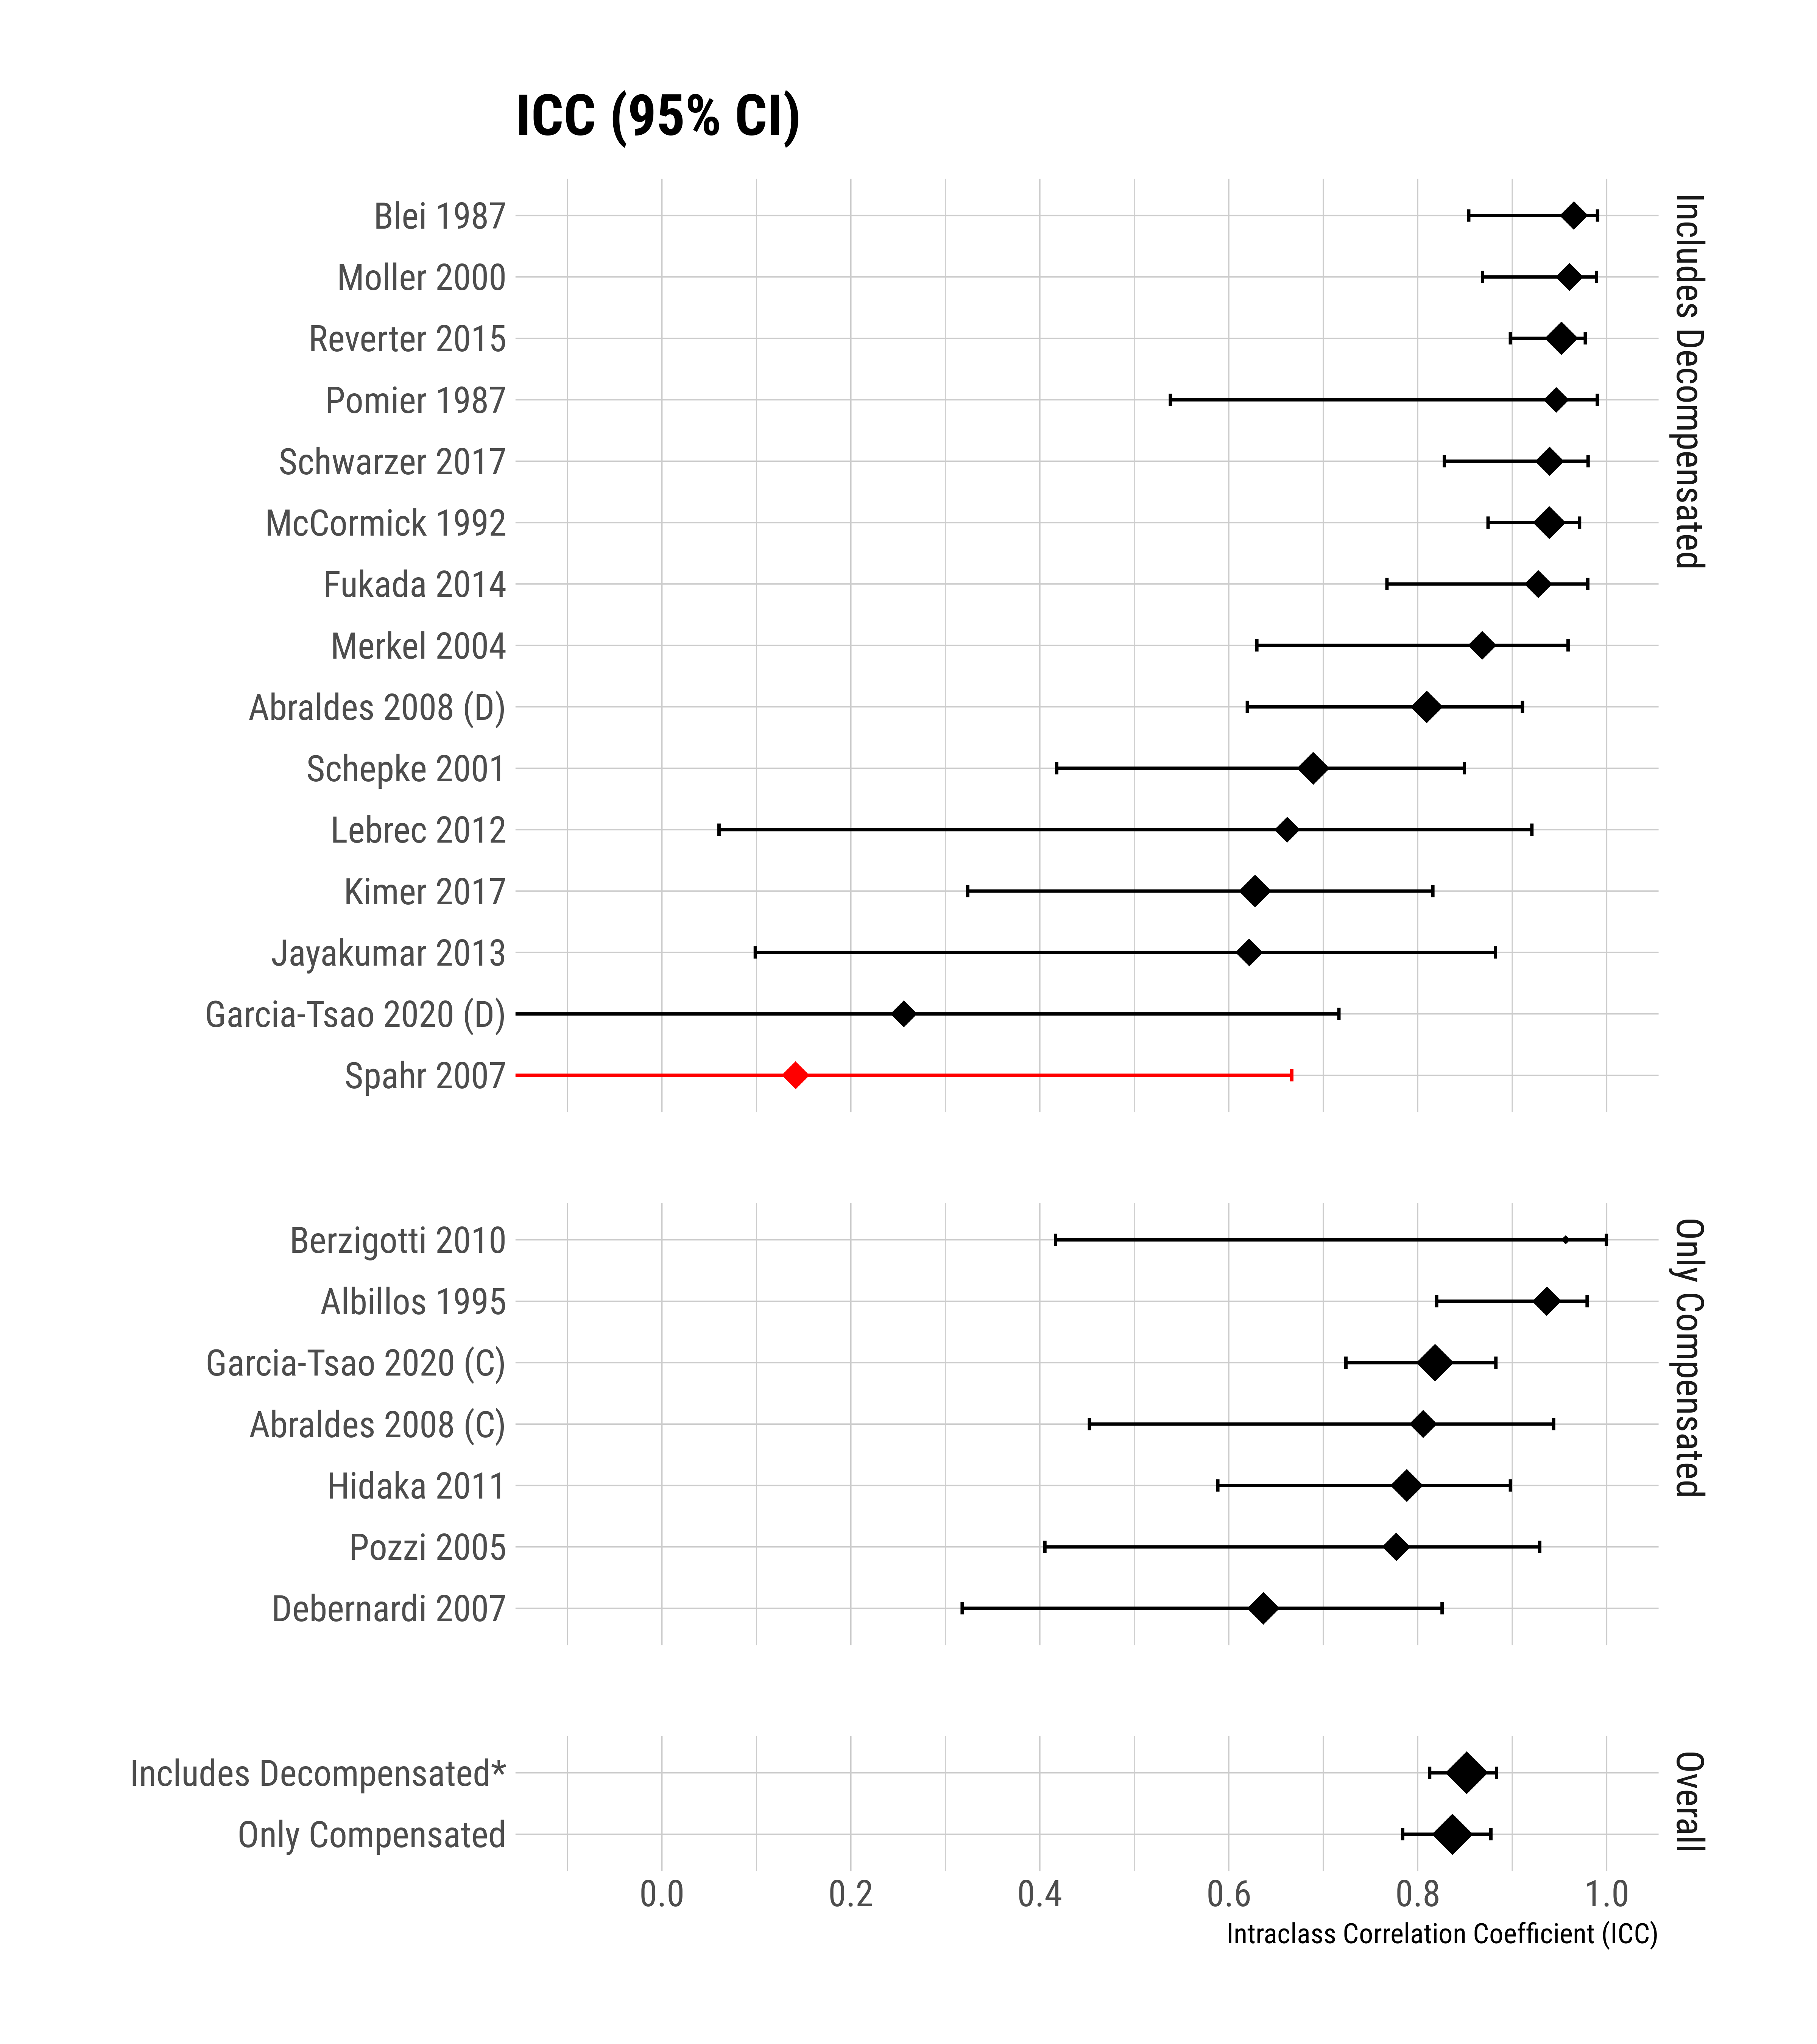
\includegraphics{figures/icc_forest-1.png}

This analysis constitutes a mega-analysis: we have all the original data
and the overall estimates are performed using the original data
estimates. However, in order to asess the study heterogeneity, I will
run a classical meta-analysis. I will perform a Fisher's z
transformation on the ICC values, perform a classic meta-analysis, and
assess the heterogeneity.

\begin{Shaded}
\begin{Highlighting}[]
\NormalTok{dat }\OtherTok{\textless{}{-}}\NormalTok{ icc\_out }\SpecialCharTok{\%\textgreater{}\%} 
  \FunctionTok{filter}\NormalTok{(Study }\SpecialCharTok{!=} \StringTok{"Spahr 2007"}\NormalTok{) }\SpecialCharTok{\%\textgreater{}\%} 
  \FunctionTok{filter}\NormalTok{(decomp }\SpecialCharTok{!=} \StringTok{"Overall"}\NormalTok{) }\SpecialCharTok{\%\textgreater{}\%} 
  \FunctionTok{filter}\NormalTok{(n }\SpecialCharTok{\textgreater{}} \DecValTok{4}\NormalTok{) }\SpecialCharTok{\%\textgreater{}\%} 
  \FunctionTok{escalc}\NormalTok{(}\AttributeTok{measure=}\StringTok{"ZCOR"}\NormalTok{, }\AttributeTok{ri=}\NormalTok{icc, }\AttributeTok{ni=}\NormalTok{n, }\AttributeTok{data=}\NormalTok{., }\AttributeTok{slab=}\NormalTok{Study) }

\NormalTok{res }\OtherTok{\textless{}{-}} \FunctionTok{rma}\NormalTok{(yi, vi, }\AttributeTok{data=}\NormalTok{dat) }
\NormalTok{res }
\end{Highlighting}
\end{Shaded}

\begin{verbatim}
## 
## Random-Effects Model (k = 20; tau^2 estimator: REML)
## 
## tau^2 (estimated amount of total heterogeneity): 0.1838 (SE = 0.0768)
## tau (square root of estimated tau^2 value):      0.4287
## I^2 (total heterogeneity / total variability):   81.58%
## H^2 (total variability / sampling variability):  5.43
## 
## Test for Heterogeneity:
## Q(df = 19) = 91.7983, p-val < .0001
## 
## Model Results:
## 
## estimate      se     zval    pval   ci.lb   ci.ub 
##   1.2674  0.1091  11.6164  <.0001  1.0536  1.4813  *** 
## 
## ---
## Signif. codes:  0 '***' 0.001 '**' 0.01 '*' 0.05 '.' 0.1 ' ' 1
\end{verbatim}

\hypertarget{sdd}{%
\subsubsection{SDD}\label{sdd}}

\hypertarget{absolute}{%
\paragraph{Absolute}\label{absolute}}

Let's have a look at the study-by-study SDD, but in raw units

\begin{Shaded}
\begin{Highlighting}[]
\NormalTok{sdd\_out }\OtherTok{\textless{}{-}} \FunctionTok{map\_df}\NormalTok{(trt\_study}\SpecialCharTok{$}\NormalTok{outcomes, }\StringTok{"sdd"}\NormalTok{) }\SpecialCharTok{\%\textgreater{}\%} 
  \FunctionTok{mutate}\NormalTok{(}\AttributeTok{Study =}\NormalTok{ trt\_study}\SpecialCharTok{$}\NormalTok{New\_Description) }\SpecialCharTok{\%\textgreater{}\%} 
  \FunctionTok{rename}\NormalTok{(}\AttributeTok{sdd=}\NormalTok{value, }\AttributeTok{sdd\_l =}\NormalTok{ lbound, }\AttributeTok{sdd\_u =}\NormalTok{ ubound) }\SpecialCharTok{\%\textgreater{}\%} 
  \FunctionTok{left\_join}\NormalTok{(studynames) }\SpecialCharTok{\%\textgreater{}\%} 
  \FunctionTok{left\_join}\NormalTok{(}\FunctionTok{select}\NormalTok{(tidytrt, Study, decomp, n)) }\SpecialCharTok{\%\textgreater{}\%} 
  \FunctionTok{left\_join}\NormalTok{(trt\_studydemog) }\SpecialCharTok{\%\textgreater{}\%} 
  \FunctionTok{mutate}\NormalTok{(}\AttributeTok{decomp =} \FunctionTok{ifelse}\NormalTok{(Perc\_Decomp }\SpecialCharTok{\textgreater{}}\DecValTok{0}\NormalTok{ , }
                           \AttributeTok{yes=}\StringTok{"Includes Decompensated"}\NormalTok{,}
                           \AttributeTok{no =} \StringTok{"Only Compensated"}\NormalTok{)) }\SpecialCharTok{\%\textgreater{}\%} 
  \FunctionTok{mutate}\NormalTok{(}\AttributeTok{decomp =} \FunctionTok{factor}\NormalTok{(decomp, }\AttributeTok{levels=}\FunctionTok{c}\NormalTok{(}
    \StringTok{"Includes Decompensated"}\NormalTok{, }\StringTok{"Only Compensated"}\NormalTok{))) }\SpecialCharTok{\%\textgreater{}\%} 
  \FunctionTok{arrange}\NormalTok{(decomp, }\FunctionTok{desc}\NormalTok{(sdd)) }\SpecialCharTok{\%\textgreater{}\%} 
  \FunctionTok{bind\_rows}\NormalTok{(overall) }\SpecialCharTok{\%\textgreater{}\%} 
  \FunctionTok{mutate}\NormalTok{(}\AttributeTok{Study =} \FunctionTok{fct\_inorder}\NormalTok{(Study))}

\NormalTok{SDDs }\OtherTok{\textless{}{-}} \FunctionTok{ggplot}\NormalTok{(sdd\_out,}\FunctionTok{aes}\NormalTok{(}\AttributeTok{x=}\NormalTok{sdd,}\AttributeTok{y=}\NormalTok{Study, }
                           \AttributeTok{colour=}\NormalTok{Catheter)) }\SpecialCharTok{+}
  \FunctionTok{facet\_grid}\NormalTok{(decomp}\SpecialCharTok{\textasciitilde{}}\NormalTok{., }\AttributeTok{scales=}\StringTok{"free"}\NormalTok{, }\AttributeTok{space=}\StringTok{"free"}\NormalTok{) }\SpecialCharTok{+}
  \FunctionTok{geom\_point}\NormalTok{(}\FunctionTok{aes}\NormalTok{(}\AttributeTok{size=}\FunctionTok{log}\NormalTok{(n)), }\AttributeTok{shape=}\DecValTok{18}\NormalTok{) }\SpecialCharTok{+} 
  \FunctionTok{scale\_x\_continuous}\NormalTok{(}\AttributeTok{breaks =} \FunctionTok{seq}\NormalTok{(}\DecValTok{0}\NormalTok{, }\DecValTok{20}\NormalTok{, }\AttributeTok{by=}\DecValTok{2}\NormalTok{))}\SpecialCharTok{+}
  \FunctionTok{geom\_errorbarh}\NormalTok{(}\FunctionTok{aes}\NormalTok{(}\AttributeTok{xmax =}\NormalTok{ sdd\_u, }\AttributeTok{xmin =}\NormalTok{ sdd\_l), }\AttributeTok{height =} \FloatTok{0.15}\NormalTok{) }\SpecialCharTok{+}
  \CommentTok{\#geom\_vline(xintercept = 1, linetype = "longdash") +}
  \FunctionTok{labs}\NormalTok{(}\AttributeTok{y=}\StringTok{""}\NormalTok{, }\AttributeTok{x=}\StringTok{"Smallest Detectable Difference (mmHg)"}\NormalTok{) }\SpecialCharTok{+}
  \FunctionTok{theme}\NormalTok{(}\AttributeTok{text =} \FunctionTok{element\_text}\NormalTok{(}\AttributeTok{size=}\DecValTok{20}\NormalTok{)) }\SpecialCharTok{+}
  \FunctionTok{ggtitle}\NormalTok{(}\StringTok{"SDD (95\% CI)"}\NormalTok{) }\SpecialCharTok{+}
  \FunctionTok{scale\_colour\_manual}\NormalTok{(}\AttributeTok{values =} \FunctionTok{c}\NormalTok{(}\StringTok{"black"}\NormalTok{, }\StringTok{"red"}\NormalTok{)) }\SpecialCharTok{+}
  \FunctionTok{guides}\NormalTok{(}\AttributeTok{colour=}\ConstantTok{FALSE}\NormalTok{, }\AttributeTok{shape=}\ConstantTok{FALSE}\NormalTok{) }\SpecialCharTok{+}
  \CommentTok{\#scale\_shape\_manual(values = c(18, 19)) +}
  \FunctionTok{coord\_cartesian}\NormalTok{(}\AttributeTok{xlim=}\FunctionTok{c}\NormalTok{(}\DecValTok{0}\NormalTok{,}\DecValTok{16}\NormalTok{)) }\SpecialCharTok{+}
  \FunctionTok{guides}\NormalTok{(}\AttributeTok{size =} \ConstantTok{FALSE}\NormalTok{) }\SpecialCharTok{+}
  \ConstantTok{NULL}

\NormalTok{SDDs  }\CommentTok{\#+ annotate("rect", xmin = 0.75, xmax = 1, ymin="Spahr 2007", ymax="Blei 1987", alpha = .2, fill="grey")}
\end{Highlighting}
\end{Shaded}

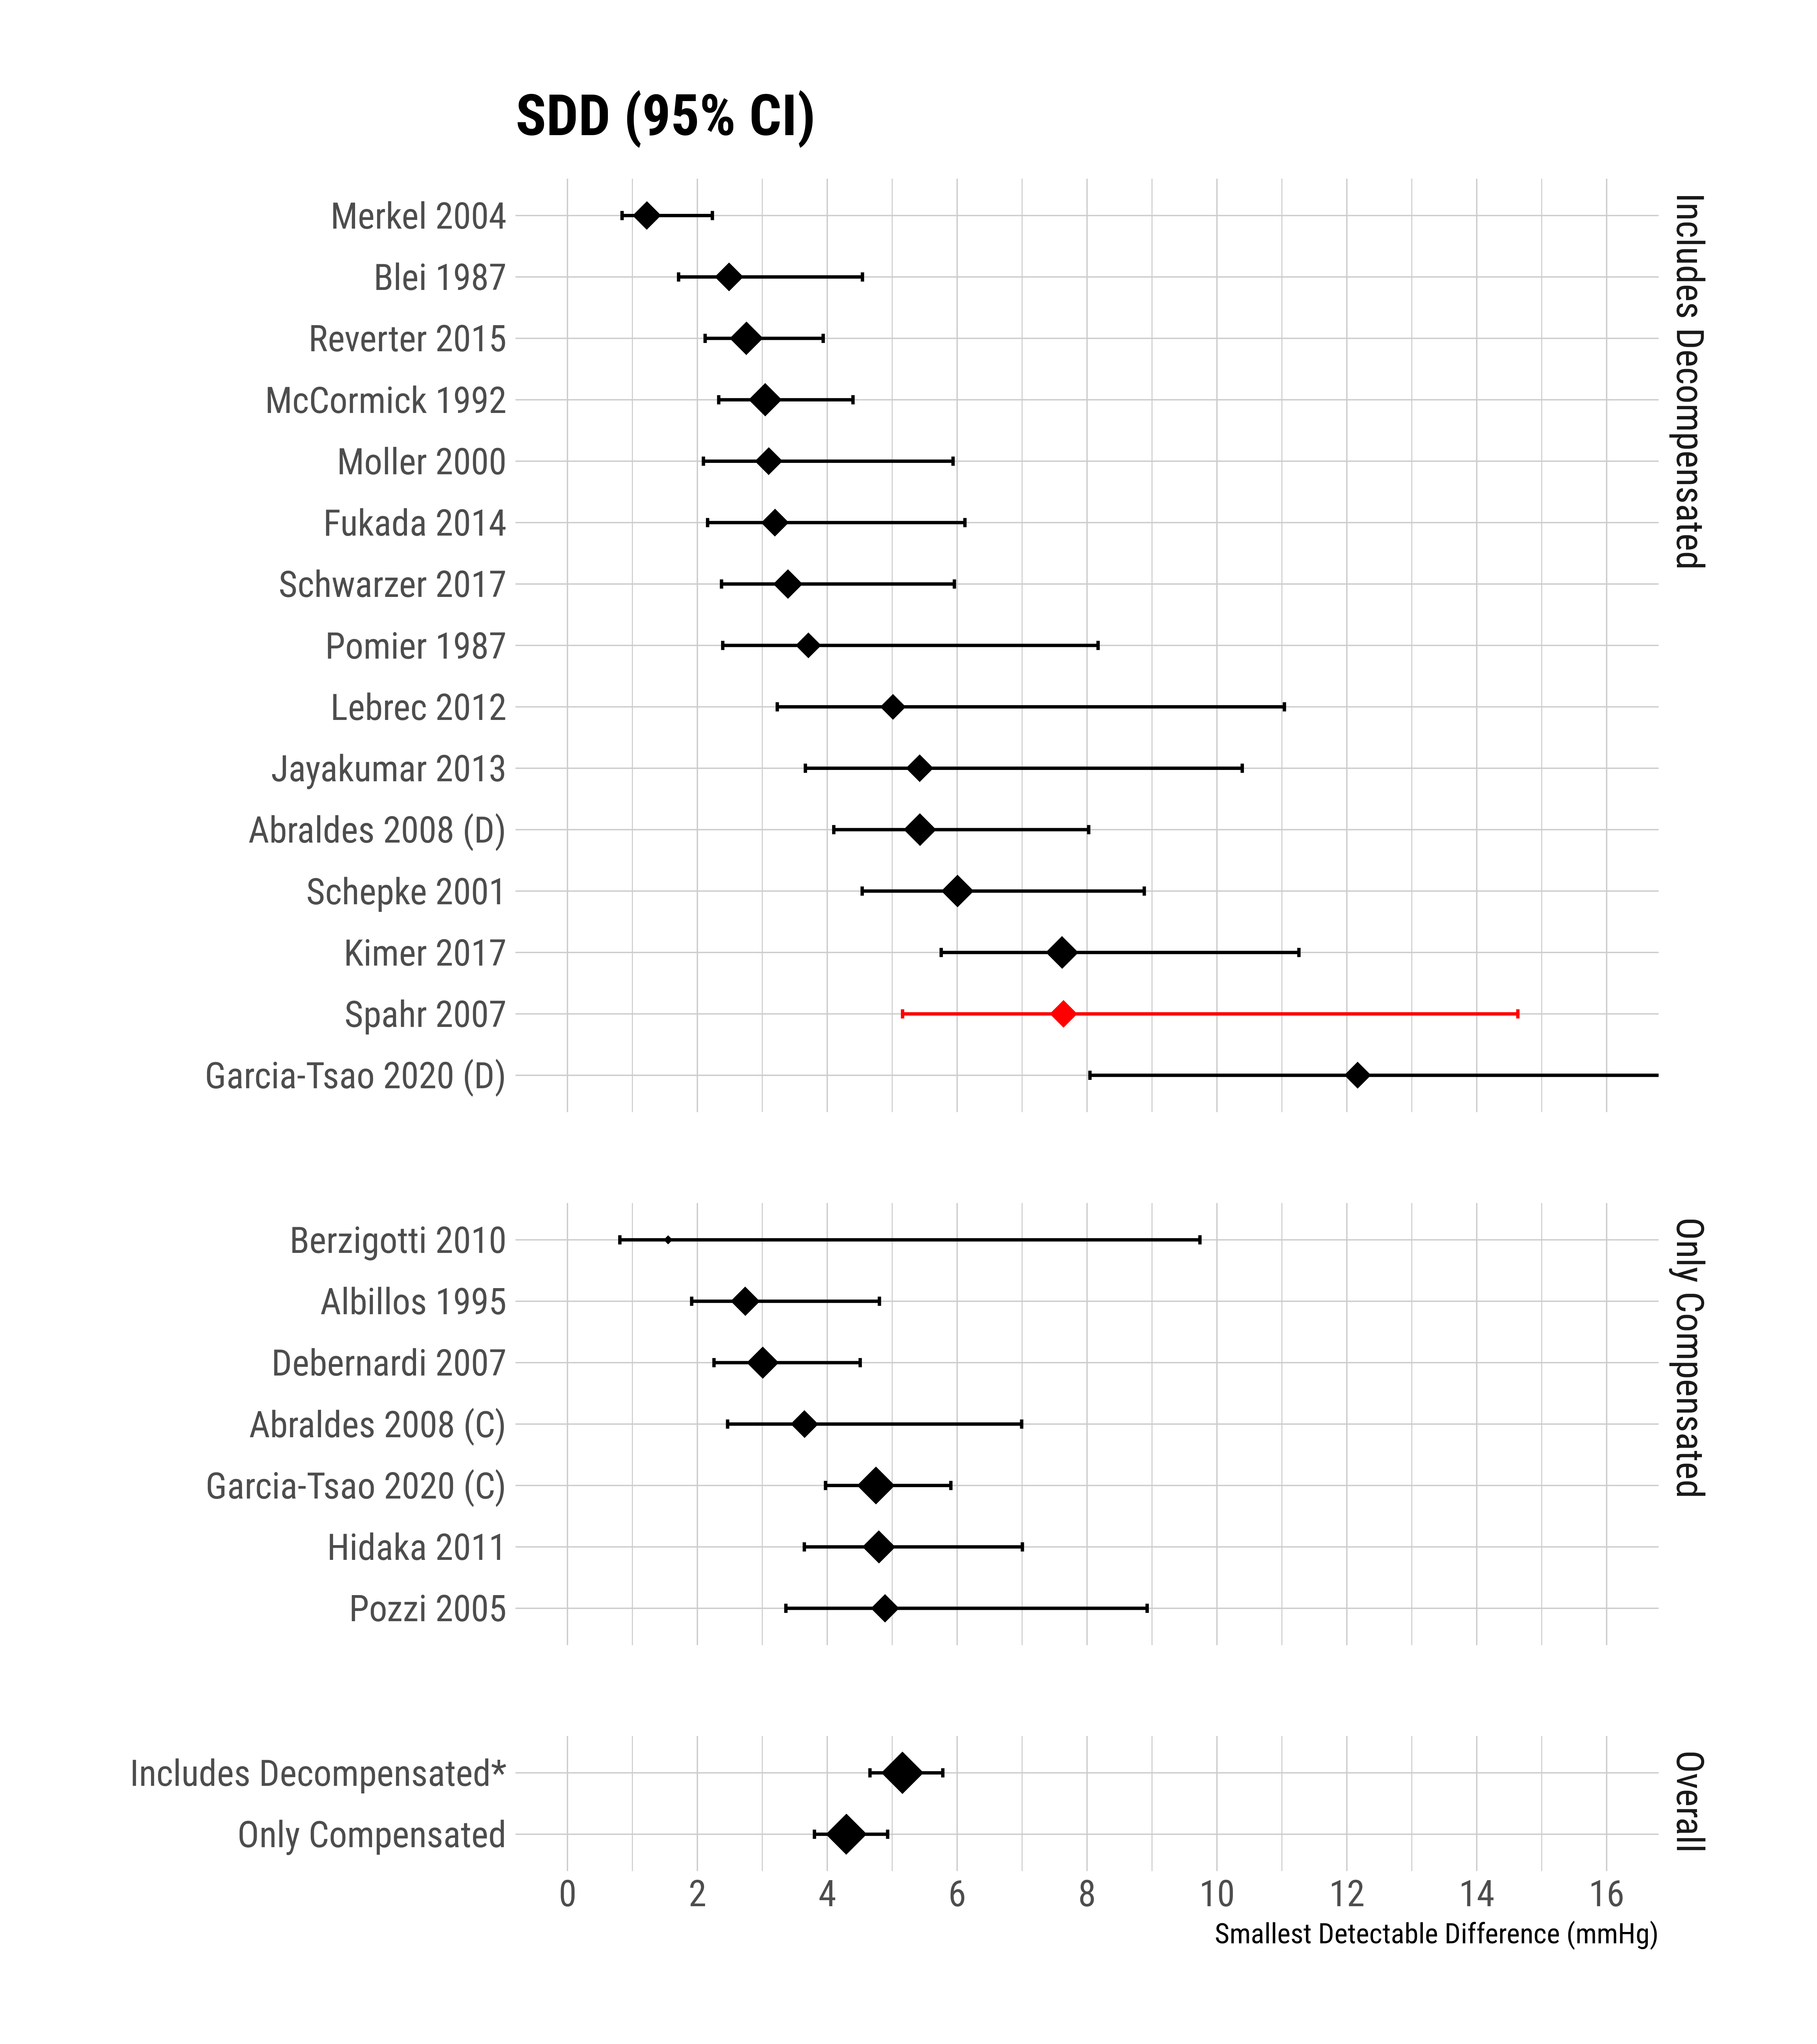
\includegraphics{figures/sdd_absolute_forest-1.png}

And here we run the meta-analysis again to assess heterogeneity. We
can't use the SDD because it has asymmetric confidence intervals, and it
cannot be Fisher's z transformed. So we can run a meta-analysis based on
the average absolute variation to test the heterogeneity.

\begin{Shaded}
\begin{Highlighting}[]
\NormalTok{dat }\OtherTok{\textless{}{-}}\NormalTok{ trt\_study }\SpecialCharTok{\%\textgreater{}\%} 
  \FunctionTok{mutate}\NormalTok{(}
    \AttributeTok{mean\_abs\_var =} \FunctionTok{map\_dbl}\NormalTok{(outcomes, }\SpecialCharTok{\textasciitilde{}}\FunctionTok{mean}\NormalTok{(}\FunctionTok{sqrt}\NormalTok{(.x}\SpecialCharTok{$}\NormalTok{absvars))),}
    \AttributeTok{se\_abs\_var =} \FunctionTok{map\_dbl}\NormalTok{(outcomes, }\SpecialCharTok{\textasciitilde{}}\FunctionTok{sd}\NormalTok{(}\FunctionTok{sqrt}\NormalTok{(.x}\SpecialCharTok{$}\NormalTok{absvars)) }\SpecialCharTok{/} \FunctionTok{sqrt}\NormalTok{(}\FunctionTok{length}\NormalTok{(.x}\SpecialCharTok{$}\NormalTok{absvars)))}
\NormalTok{  ) }\SpecialCharTok{\%\textgreater{}\%} 
  \FunctionTok{filter}\NormalTok{(New\_Description }\SpecialCharTok{!=} \StringTok{"Spahr 2007"}\NormalTok{) }\SpecialCharTok{\%\textgreater{}\%} 
  \FunctionTok{ungroup}\NormalTok{() }\SpecialCharTok{\%\textgreater{}\%} 
  \FunctionTok{mutate}\NormalTok{(}
    \AttributeTok{yi =}\NormalTok{ mean\_abs\_var,}
    \AttributeTok{vi =}\NormalTok{ se\_abs\_var}\SpecialCharTok{\^{}}\DecValTok{2}\NormalTok{) }\SpecialCharTok{\%\textgreater{}\%} 
  \FunctionTok{select}\NormalTok{(}\SpecialCharTok{{-}}\NormalTok{data, }\SpecialCharTok{{-}}\NormalTok{outcomes) }\SpecialCharTok{\%\textgreater{}\%} 
  \FunctionTok{escalc}\NormalTok{(}\AttributeTok{measure=}\StringTok{"MN"}\NormalTok{, }\AttributeTok{yi=}\NormalTok{yi, }\AttributeTok{vi=}\NormalTok{vi, }\AttributeTok{ni=}\NormalTok{n, }\AttributeTok{data=}\NormalTok{., }\AttributeTok{slab=}\NormalTok{New\_Description) }

\NormalTok{transf.sqrt }\OtherTok{\textless{}{-}} \ControlFlowTok{function}\NormalTok{ (xi, ...) }
\NormalTok{\{}
\NormalTok{    zi }\OtherTok{\textless{}{-}} \FunctionTok{sqrt}\NormalTok{(xi)}
\NormalTok{    zi[xi }\SpecialCharTok{\textless{}} \DecValTok{0}\NormalTok{] }\OtherTok{\textless{}{-}} \DecValTok{0}
    \FunctionTok{return}\NormalTok{(}\FunctionTok{c}\NormalTok{(zi))}
\NormalTok{\}}

\NormalTok{res }\OtherTok{\textless{}{-}} \FunctionTok{rma}\NormalTok{(yi, vi, }\AttributeTok{data=}\NormalTok{dat)}
\NormalTok{res }
\end{Highlighting}
\end{Shaded}

\begin{verbatim}
## 
## Random-Effects Model (k = 21; tau^2 estimator: REML)
## 
## tau^2 (estimated amount of total heterogeneity): 0.0016 (SE = 0.0010)
## tau (square root of estimated tau^2 value):      0.0405
## I^2 (total heterogeneity / total variability):   54.64%
## H^2 (total variability / sampling variability):  2.20
## 
## Test for Heterogeneity:
## Q(df = 20) = 46.5104, p-val = 0.0007
## 
## Model Results:
## 
## estimate      se     zval    pval   ci.lb   ci.ub 
##   0.2572  0.0128  20.1232  <.0001  0.2322  0.2823  *** 
## 
## ---
## Signif. codes:  0 '***' 0.001 '**' 0.01 '*' 0.05 '.' 0.1 ' ' 1
\end{verbatim}

\hypertarget{percentage}{%
\paragraph{Percentage}\label{percentage}}

Now the study-by-study SDD, but in percentages

\begin{Shaded}
\begin{Highlighting}[]
\NormalTok{sddm\_out }\OtherTok{\textless{}{-}} \FunctionTok{map\_df}\NormalTok{(trt\_study}\SpecialCharTok{$}\NormalTok{outcomes, }\StringTok{"sddm"}\NormalTok{) }\SpecialCharTok{\%\textgreater{}\%} 
  \FunctionTok{mutate}\NormalTok{(}\AttributeTok{Study =}\NormalTok{ trt\_study}\SpecialCharTok{$}\NormalTok{New\_Description) }\SpecialCharTok{\%\textgreater{}\%} 
  \FunctionTok{rename}\NormalTok{(}\AttributeTok{sddm=}\NormalTok{value, }\AttributeTok{sddm\_l =}\NormalTok{ lbound, }\AttributeTok{sddm\_u =}\NormalTok{ ubound) }\SpecialCharTok{\%\textgreater{}\%} 
  \FunctionTok{mutate}\NormalTok{(}\AttributeTok{sddm=}\DecValTok{100}\SpecialCharTok{*}\NormalTok{sddm, }\AttributeTok{sddm\_l =} \DecValTok{100}\SpecialCharTok{*}\NormalTok{sddm\_l, }\AttributeTok{sddm\_u =} \DecValTok{100}\SpecialCharTok{*}\NormalTok{sddm\_u) }\SpecialCharTok{\%\textgreater{}\%} 
  \FunctionTok{left\_join}\NormalTok{(studynames) }\SpecialCharTok{\%\textgreater{}\%} 
  \FunctionTok{left\_join}\NormalTok{(}\FunctionTok{select}\NormalTok{(tidytrt, Study, decomp, n)) }\SpecialCharTok{\%\textgreater{}\%} 
  \FunctionTok{left\_join}\NormalTok{(trt\_studydemog) }\SpecialCharTok{\%\textgreater{}\%} 
  \FunctionTok{mutate}\NormalTok{(}\AttributeTok{decomp =} \FunctionTok{ifelse}\NormalTok{(Perc\_Decomp }\SpecialCharTok{\textgreater{}}\DecValTok{0}\NormalTok{ , }
                           \AttributeTok{yes=}\StringTok{"Includes Decompensated"}\NormalTok{,}
                           \AttributeTok{no =} \StringTok{"Only Compensated"}\NormalTok{)) }\SpecialCharTok{\%\textgreater{}\%} 
  \FunctionTok{mutate}\NormalTok{(}\AttributeTok{decomp =} \FunctionTok{factor}\NormalTok{(decomp, }\AttributeTok{levels=}\FunctionTok{c}\NormalTok{(}
    \StringTok{"Includes Decompensated"}\NormalTok{, }\StringTok{"Only Compensated"}\NormalTok{))) }\SpecialCharTok{\%\textgreater{}\%} 
  \FunctionTok{arrange}\NormalTok{(decomp, }\FunctionTok{desc}\NormalTok{(sddm)) }\SpecialCharTok{\%\textgreater{}\%} 
  \FunctionTok{bind\_rows}\NormalTok{(overall) }\SpecialCharTok{\%\textgreater{}\%} 
  \FunctionTok{mutate}\NormalTok{(}\AttributeTok{Study =} \FunctionTok{fct\_inorder}\NormalTok{(Study))}

\NormalTok{SDDms }\OtherTok{\textless{}{-}} \FunctionTok{ggplot}\NormalTok{(sddm\_out,}\FunctionTok{aes}\NormalTok{(}\AttributeTok{x=}\NormalTok{sddm,}\AttributeTok{y=}\NormalTok{Study, }
                           \AttributeTok{colour=}\NormalTok{Catheter)) }\SpecialCharTok{+}
  \FunctionTok{facet\_grid}\NormalTok{(decomp}\SpecialCharTok{\textasciitilde{}}\NormalTok{., }\AttributeTok{scales=}\StringTok{"free"}\NormalTok{, }\AttributeTok{space=}\StringTok{"free"}\NormalTok{) }\SpecialCharTok{+}
  \FunctionTok{geom\_point}\NormalTok{(}\FunctionTok{aes}\NormalTok{(}\AttributeTok{size=}\FunctionTok{log}\NormalTok{(n)), }\AttributeTok{shape=}\DecValTok{18}\NormalTok{) }\SpecialCharTok{+} 
  \FunctionTok{scale\_x\_continuous}\NormalTok{(}\AttributeTok{breaks =} \FunctionTok{seq}\NormalTok{(}\DecValTok{0}\NormalTok{, }\DecValTok{80}\NormalTok{, }\AttributeTok{by=}\DecValTok{10}\NormalTok{))}\SpecialCharTok{+}
  \FunctionTok{geom\_errorbarh}\NormalTok{(}\FunctionTok{aes}\NormalTok{(}\AttributeTok{xmax =}\NormalTok{ sddm\_u, }\AttributeTok{xmin =}\NormalTok{ sddm\_l), }\AttributeTok{height =} \FloatTok{0.15}\NormalTok{) }\SpecialCharTok{+}
  \CommentTok{\#geom\_vline(xintercept = 1, linetype = "longdash") +}
  \FunctionTok{labs}\NormalTok{(}\AttributeTok{y=}\StringTok{""}\NormalTok{, }\AttributeTok{x=}\StringTok{"Smallest Detectable Difference (\%mmHg)"}\NormalTok{) }\SpecialCharTok{+}
  \FunctionTok{theme}\NormalTok{(}\AttributeTok{text =} \FunctionTok{element\_text}\NormalTok{(}\AttributeTok{size=}\DecValTok{20}\NormalTok{)) }\SpecialCharTok{+}
  \FunctionTok{ggtitle}\NormalTok{(}\StringTok{"\%SDD (95\% CI)"}\NormalTok{) }\SpecialCharTok{+}
  \FunctionTok{scale\_colour\_manual}\NormalTok{(}\AttributeTok{values =} \FunctionTok{c}\NormalTok{(}\StringTok{"black"}\NormalTok{, }\StringTok{"red"}\NormalTok{)) }\SpecialCharTok{+}
  \FunctionTok{guides}\NormalTok{(}\AttributeTok{colour=}\ConstantTok{FALSE}\NormalTok{, }\AttributeTok{shape=}\ConstantTok{FALSE}\NormalTok{) }\SpecialCharTok{+}
  \CommentTok{\#scale\_shape\_manual(values = c(18, 19)) +}
  \FunctionTok{coord\_cartesian}\NormalTok{(}\AttributeTok{xlim=}\FunctionTok{c}\NormalTok{(}\DecValTok{0}\NormalTok{,}\DecValTok{80}\NormalTok{)) }\SpecialCharTok{+}
  \FunctionTok{guides}\NormalTok{(}\AttributeTok{size =} \ConstantTok{FALSE}\NormalTok{) }\SpecialCharTok{+}
  \ConstantTok{NULL}

\NormalTok{SDDms  }\CommentTok{\#+ annotate("rect", xmin = 0.75, xmax = 1, ymin="Spahr 2007", ymax="Blei 1987", alpha = .2, fill="grey")}
\end{Highlighting}
\end{Shaded}

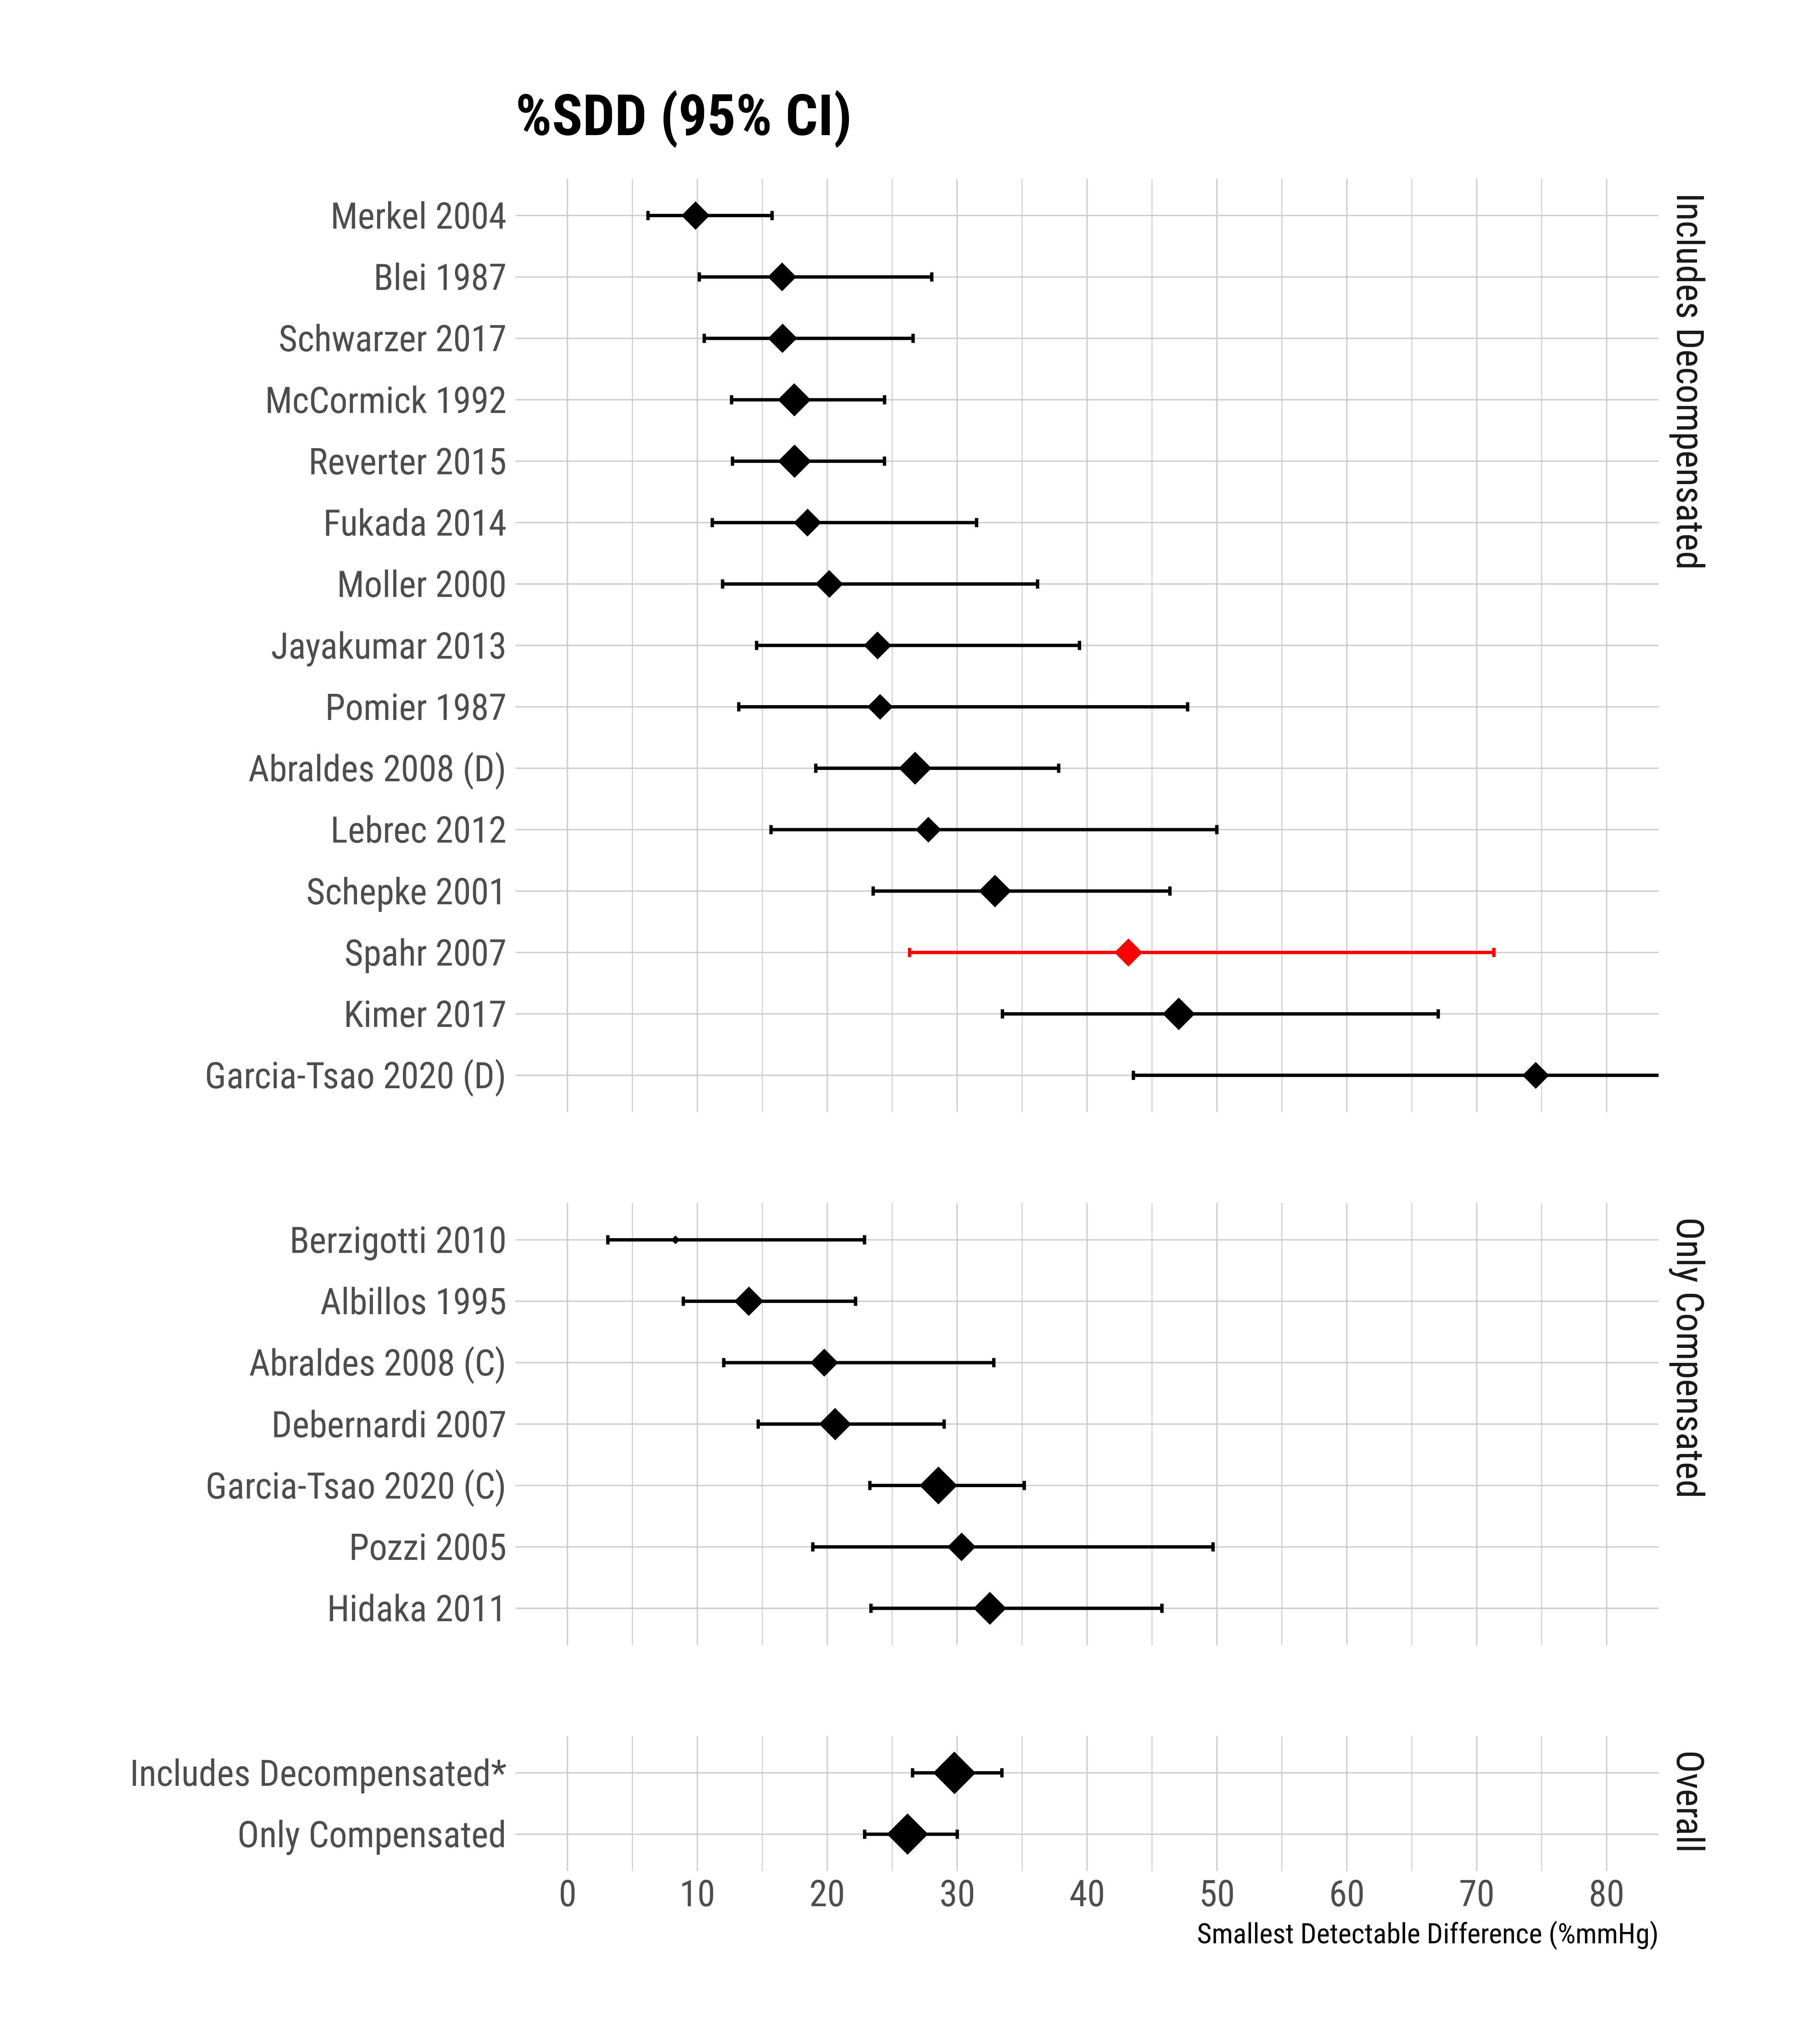
\includegraphics{figures/sdd_perc_forest-1.png}

And here we run the meta-analysis to assess heterogeneity. We can't use
the SDD\% because it has asymmetric confidence intervals, and it cannot
be Fisher's z transformed. So we can run a meta-analysis based on the
average absolute percentage variation to test the heterogeneity.

\begin{Shaded}
\begin{Highlighting}[]
\NormalTok{dat }\OtherTok{\textless{}{-}}\NormalTok{ trt\_study }\SpecialCharTok{\%\textgreater{}\%} 
  \FunctionTok{mutate}\NormalTok{(}
    \AttributeTok{mean\_abs\_var =} \FunctionTok{map\_dbl}\NormalTok{(outcomes, }\SpecialCharTok{\textasciitilde{}}\FunctionTok{mean}\NormalTok{(}\FunctionTok{sqrt}\NormalTok{(.x}\SpecialCharTok{$}\NormalTok{absvars }\SpecialCharTok{/}\NormalTok{ .x}\SpecialCharTok{$}\NormalTok{means))),}
    \AttributeTok{se\_abs\_var =} \FunctionTok{map\_dbl}\NormalTok{(outcomes, }\SpecialCharTok{\textasciitilde{}}\FunctionTok{sd}\NormalTok{(}\FunctionTok{sqrt}\NormalTok{(.x}\SpecialCharTok{$}\NormalTok{absvars }\SpecialCharTok{/}\NormalTok{ .x}\SpecialCharTok{$}\NormalTok{means)) }\SpecialCharTok{/} 
                           \FunctionTok{sqrt}\NormalTok{(}\FunctionTok{length}\NormalTok{(.x}\SpecialCharTok{$}\NormalTok{absvars)))}
\NormalTok{  ) }\SpecialCharTok{\%\textgreater{}\%} 
  \FunctionTok{filter}\NormalTok{(New\_Description }\SpecialCharTok{!=} \StringTok{"Spahr 2007"}\NormalTok{) }\SpecialCharTok{\%\textgreater{}\%} 
  \FunctionTok{ungroup}\NormalTok{() }\SpecialCharTok{\%\textgreater{}\%} 
  \FunctionTok{mutate}\NormalTok{(}
    \AttributeTok{yi =}\NormalTok{ mean\_abs\_var,}
    \AttributeTok{vi =}\NormalTok{ se\_abs\_var}\SpecialCharTok{\^{}}\DecValTok{2}\NormalTok{)}

\NormalTok{res }\OtherTok{\textless{}{-}} \FunctionTok{rma}\NormalTok{(yi, vi, }\AttributeTok{data=}\NormalTok{dat) }
\NormalTok{res }
\end{Highlighting}
\end{Shaded}

\begin{verbatim}
## 
## Random-Effects Model (k = 21; tau^2 estimator: REML)
## 
## tau^2 (estimated amount of total heterogeneity): 0.0001 (SE = 0.0001)
## tau (square root of estimated tau^2 value):      0.0107
## I^2 (total heterogeneity / total variability):   60.82%
## H^2 (total variability / sampling variability):  2.55
## 
## Test for Heterogeneity:
## Q(df = 20) = 60.4345, p-val < .0001
## 
## Model Results:
## 
## estimate      se     zval    pval   ci.lb   ci.ub 
##   0.0628  0.0033  18.8998  <.0001  0.0563  0.0694  *** 
## 
## ---
## Signif. codes:  0 '***' 0.001 '**' 0.01 '*' 0.05 '.' 0.1 ' ' 1
\end{verbatim}

\hypertarget{figures-together}{%
\subsubsection{Figures together}\label{figures-together}}

\begin{Shaded}
\begin{Highlighting}[]
\NormalTok{SDD\_together }\OtherTok{\textless{}{-}}\NormalTok{ cowplot}\SpecialCharTok{::}\FunctionTok{plot\_grid}\NormalTok{(SDDs, SDDms, }\AttributeTok{ncol =} \DecValTok{2}\NormalTok{,}
                                   \AttributeTok{labels =} \FunctionTok{c}\NormalTok{(}\StringTok{"B"}\NormalTok{, }\StringTok{"C"}\NormalTok{),}
                                   \AttributeTok{label\_size =} \DecValTok{30}\NormalTok{)}

\NormalTok{SDD\_together}
\end{Highlighting}
\end{Shaded}

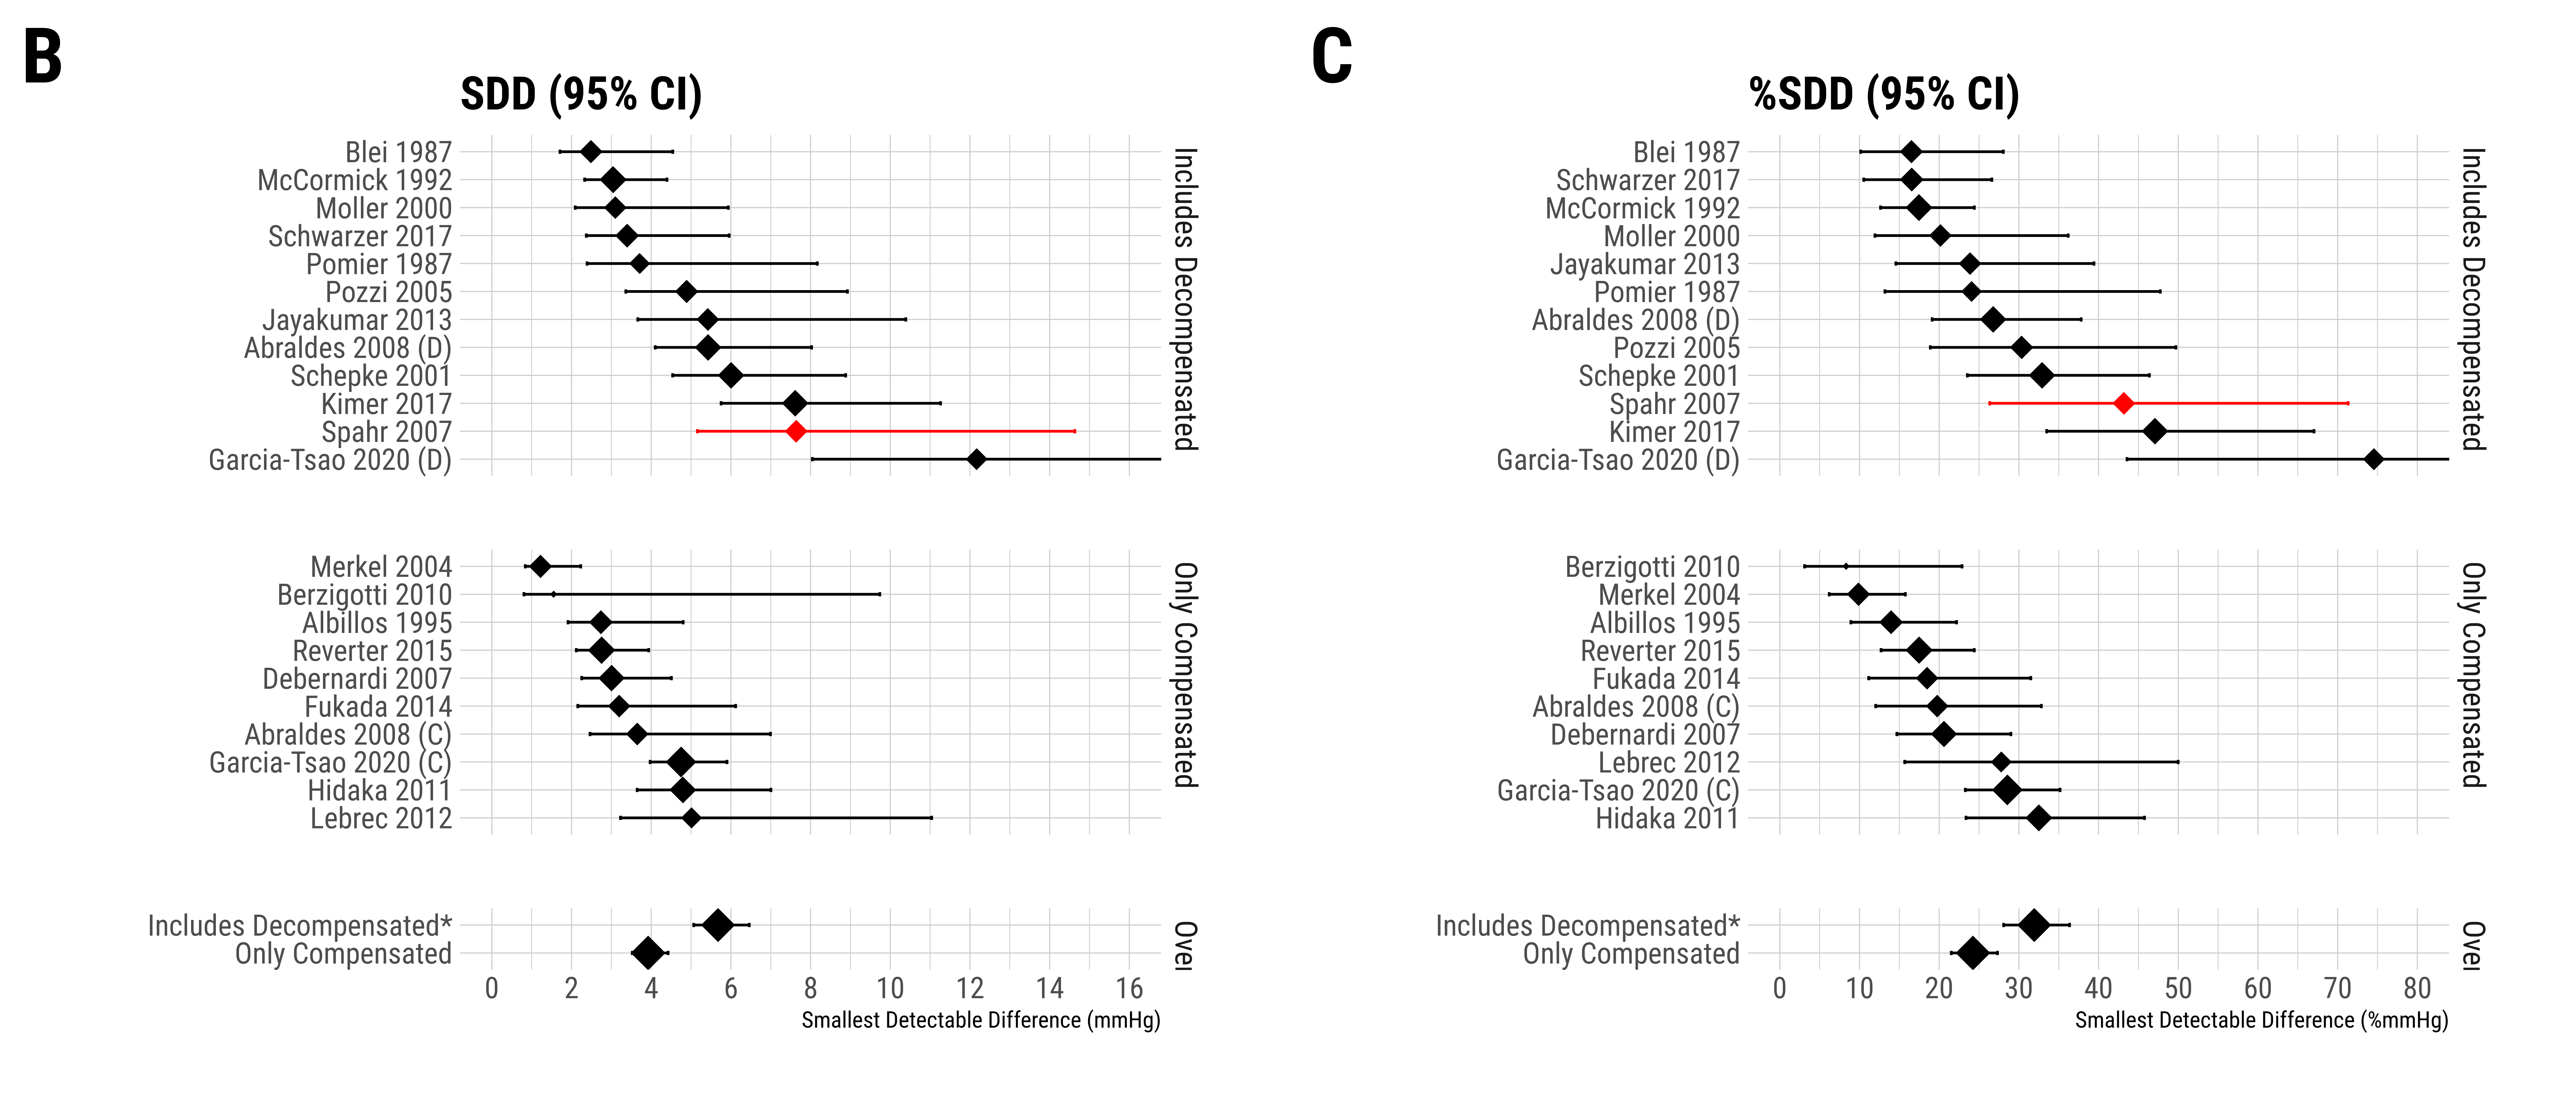
\includegraphics{figures/sdd_together_forests-1.png}

Alternatively, all in a row

\begin{Shaded}
\begin{Highlighting}[]
\NormalTok{ICCs\_row }\OtherTok{\textless{}{-}}\NormalTok{ ICCs }\SpecialCharTok{+} \FunctionTok{guides}\NormalTok{(}\AttributeTok{colour=}\ConstantTok{FALSE}\NormalTok{, }\AttributeTok{shape=}\ConstantTok{FALSE}\NormalTok{)}

\NormalTok{forest\_legend }\OtherTok{\textless{}{-}} \FunctionTok{get\_legend}\NormalTok{(ICCs }\SpecialCharTok{+} 
                              \FunctionTok{theme}\NormalTok{(}\AttributeTok{legend.position=}\StringTok{"bottom"}\NormalTok{) }\SpecialCharTok{+}
                              \FunctionTok{scale\_shape\_discrete}\NormalTok{(}\StringTok{"Patients:"}\NormalTok{) }\SpecialCharTok{+}
                              \FunctionTok{scale\_colour\_manual}\NormalTok{(}\StringTok{"Catheter:"}\NormalTok{,}
                                \AttributeTok{values=}\FunctionTok{c}\NormalTok{(}\StringTok{"black"}\NormalTok{, }\StringTok{"red"}\NormalTok{)))}

\NormalTok{forest\_row\_legendless }\OtherTok{\textless{}{-}} \FunctionTok{plot\_grid}\NormalTok{(ICCs\_row, SDDs, SDDms,}
          \AttributeTok{nrow=}\DecValTok{1}\NormalTok{, }\AttributeTok{labels=}\FunctionTok{c}\NormalTok{(}\StringTok{"A"}\NormalTok{, }\StringTok{"B"}\NormalTok{, }\StringTok{"C"}\NormalTok{), }
          \AttributeTok{label\_size=}\DecValTok{30}\NormalTok{)}

\NormalTok{forest\_row }\OtherTok{\textless{}{-}} \FunctionTok{plot\_grid}\NormalTok{(forest\_row\_legendless, forest\_legend,}
                        \AttributeTok{nrow=}\DecValTok{2}\NormalTok{, }\AttributeTok{rel\_heights =} \FunctionTok{c}\NormalTok{(}\DecValTok{15}\NormalTok{,}\DecValTok{1}\NormalTok{))}

\NormalTok{forest\_row}
\end{Highlighting}
\end{Shaded}

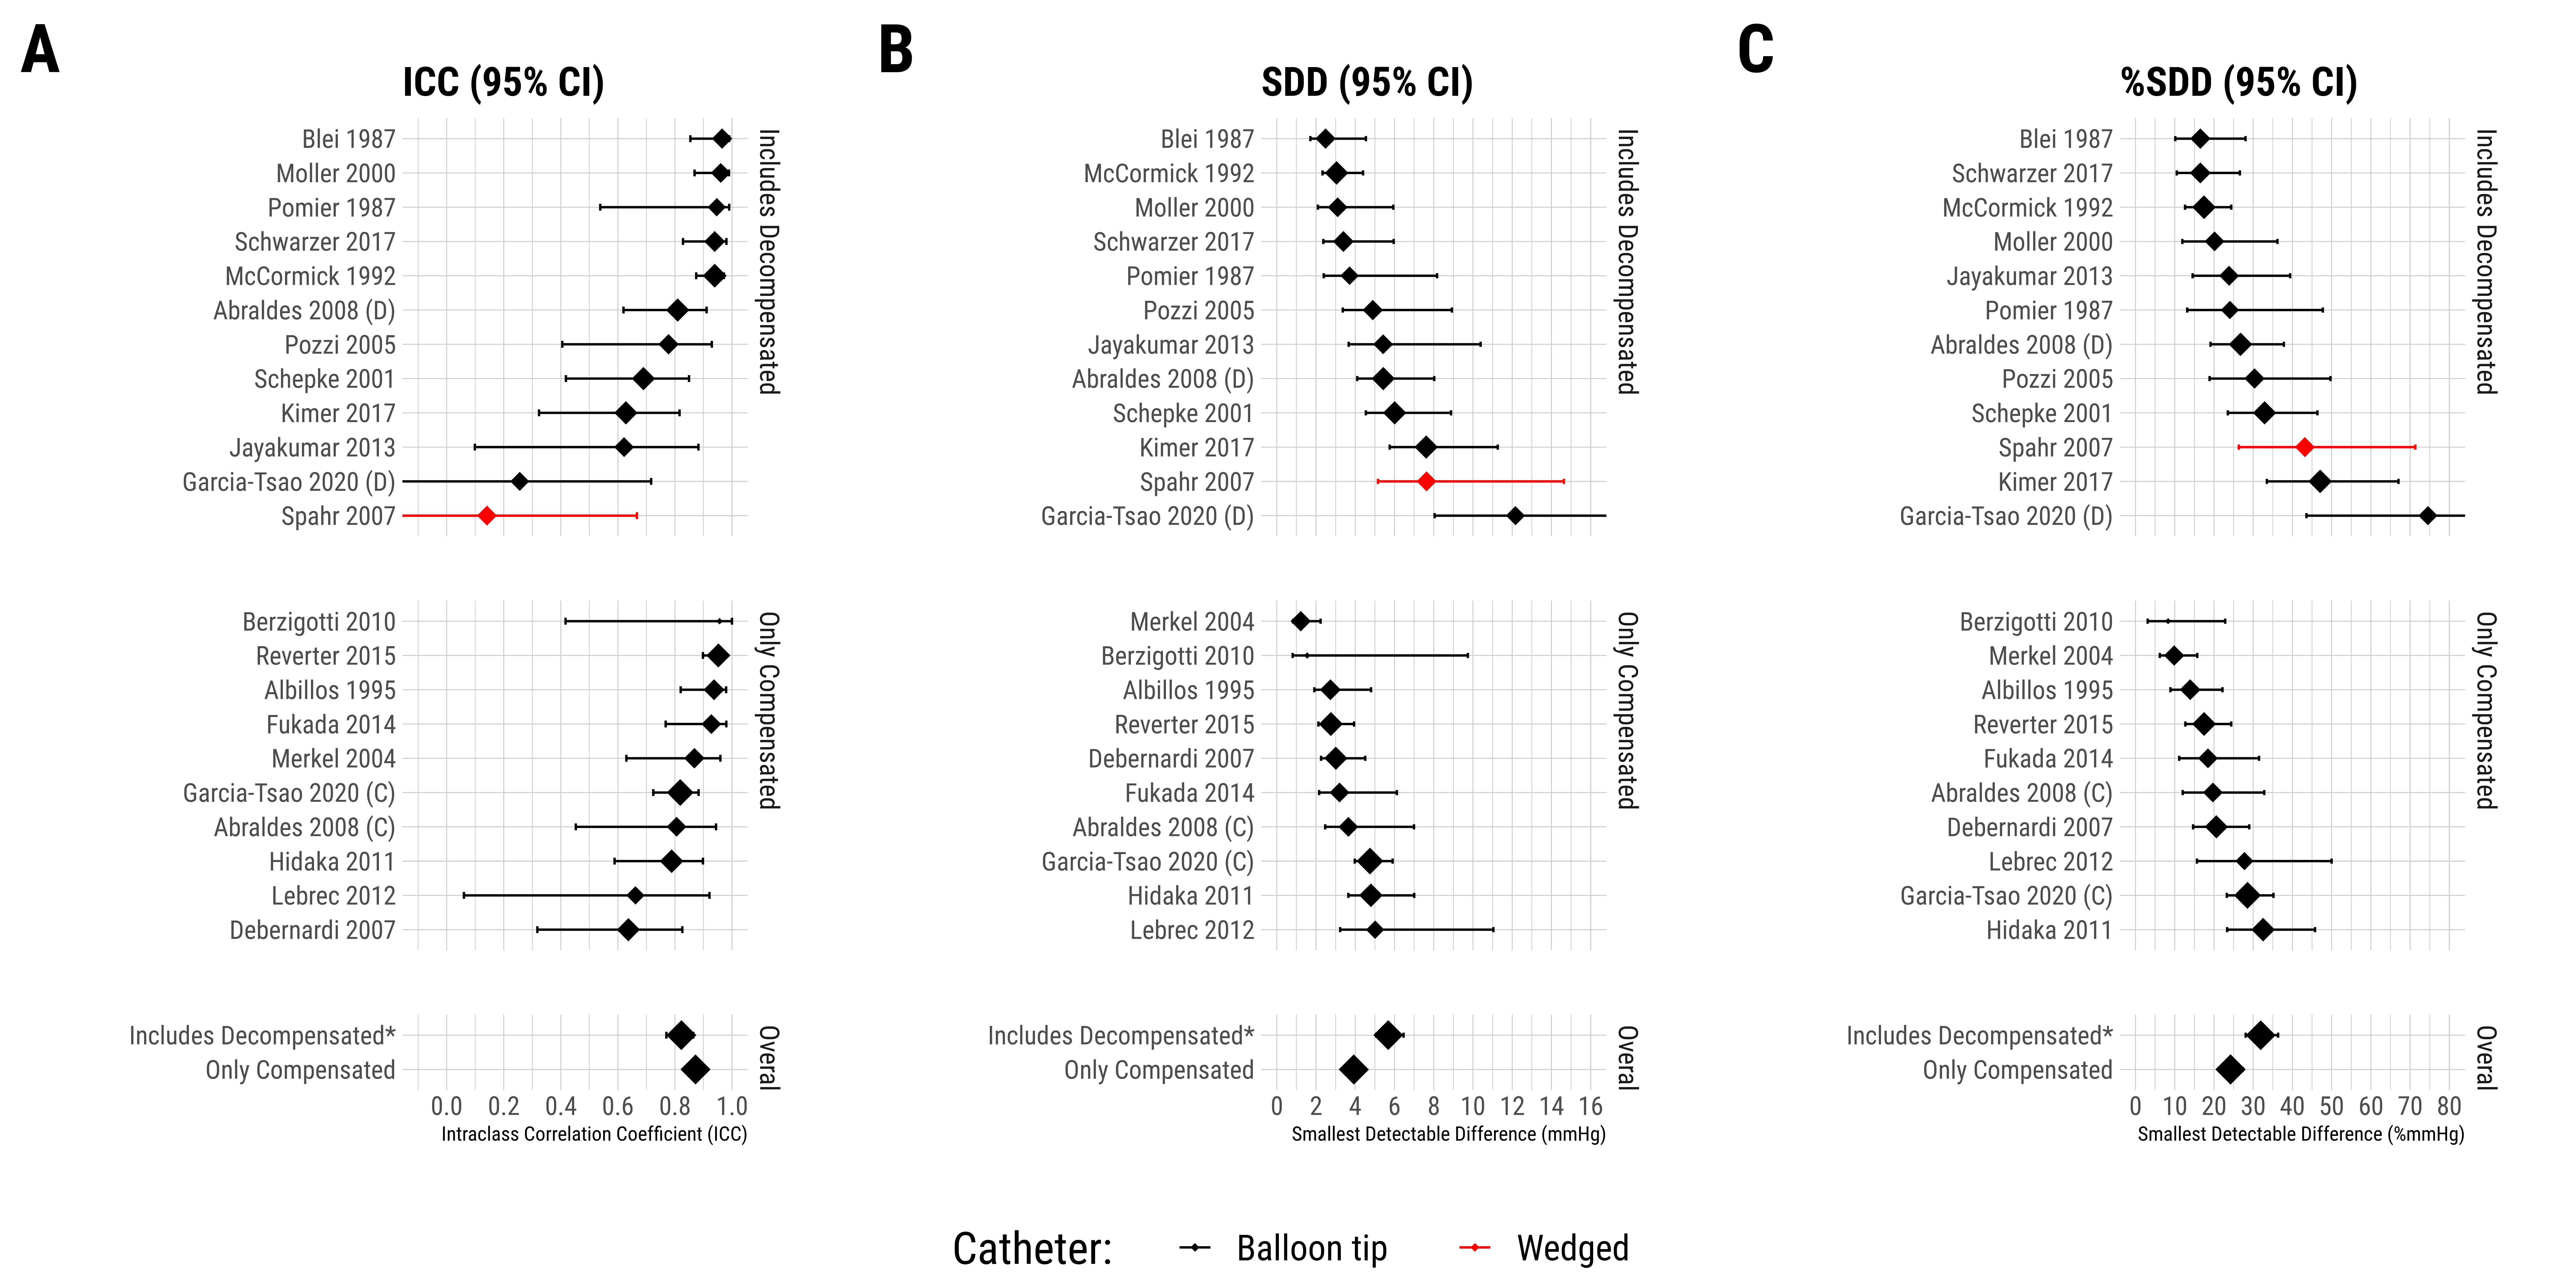
\includegraphics{figures/all_forest_row-1.png}

\begin{Shaded}
\begin{Highlighting}[]
\FunctionTok{ggsave}\NormalTok{(forest\_row, }\AttributeTok{filename =} \StringTok{"figures/forest\_three\_row.png"}\NormalTok{, }\AttributeTok{width =} \DecValTok{16}\NormalTok{, }\AttributeTok{height =} \DecValTok{8}\NormalTok{)}
\end{Highlighting}
\end{Shaded}

\hypertarget{just-icc-and-sdd}{%
\subsubsection{Just ICC and SDD}\label{just-icc-and-sdd}}

\begin{Shaded}
\begin{Highlighting}[]
\NormalTok{forest\_row2\_legendless }\OtherTok{\textless{}{-}} \FunctionTok{plot\_grid}\NormalTok{(ICCs\_row, SDDs,}
          \AttributeTok{nrow=}\DecValTok{1}\NormalTok{, }\AttributeTok{labels=}\FunctionTok{c}\NormalTok{(}\StringTok{"A"}\NormalTok{, }\StringTok{"B"}\NormalTok{), }
          \AttributeTok{label\_size=}\DecValTok{30}\NormalTok{)}

\NormalTok{forest\_row2 }\OtherTok{\textless{}{-}} \FunctionTok{plot\_grid}\NormalTok{(forest\_row2\_legendless, forest\_legend,}
                        \AttributeTok{nrow=}\DecValTok{2}\NormalTok{, }\AttributeTok{rel\_heights =} \FunctionTok{c}\NormalTok{(}\DecValTok{15}\NormalTok{,}\DecValTok{1}\NormalTok{))}

\NormalTok{forest\_row2}
\end{Highlighting}
\end{Shaded}

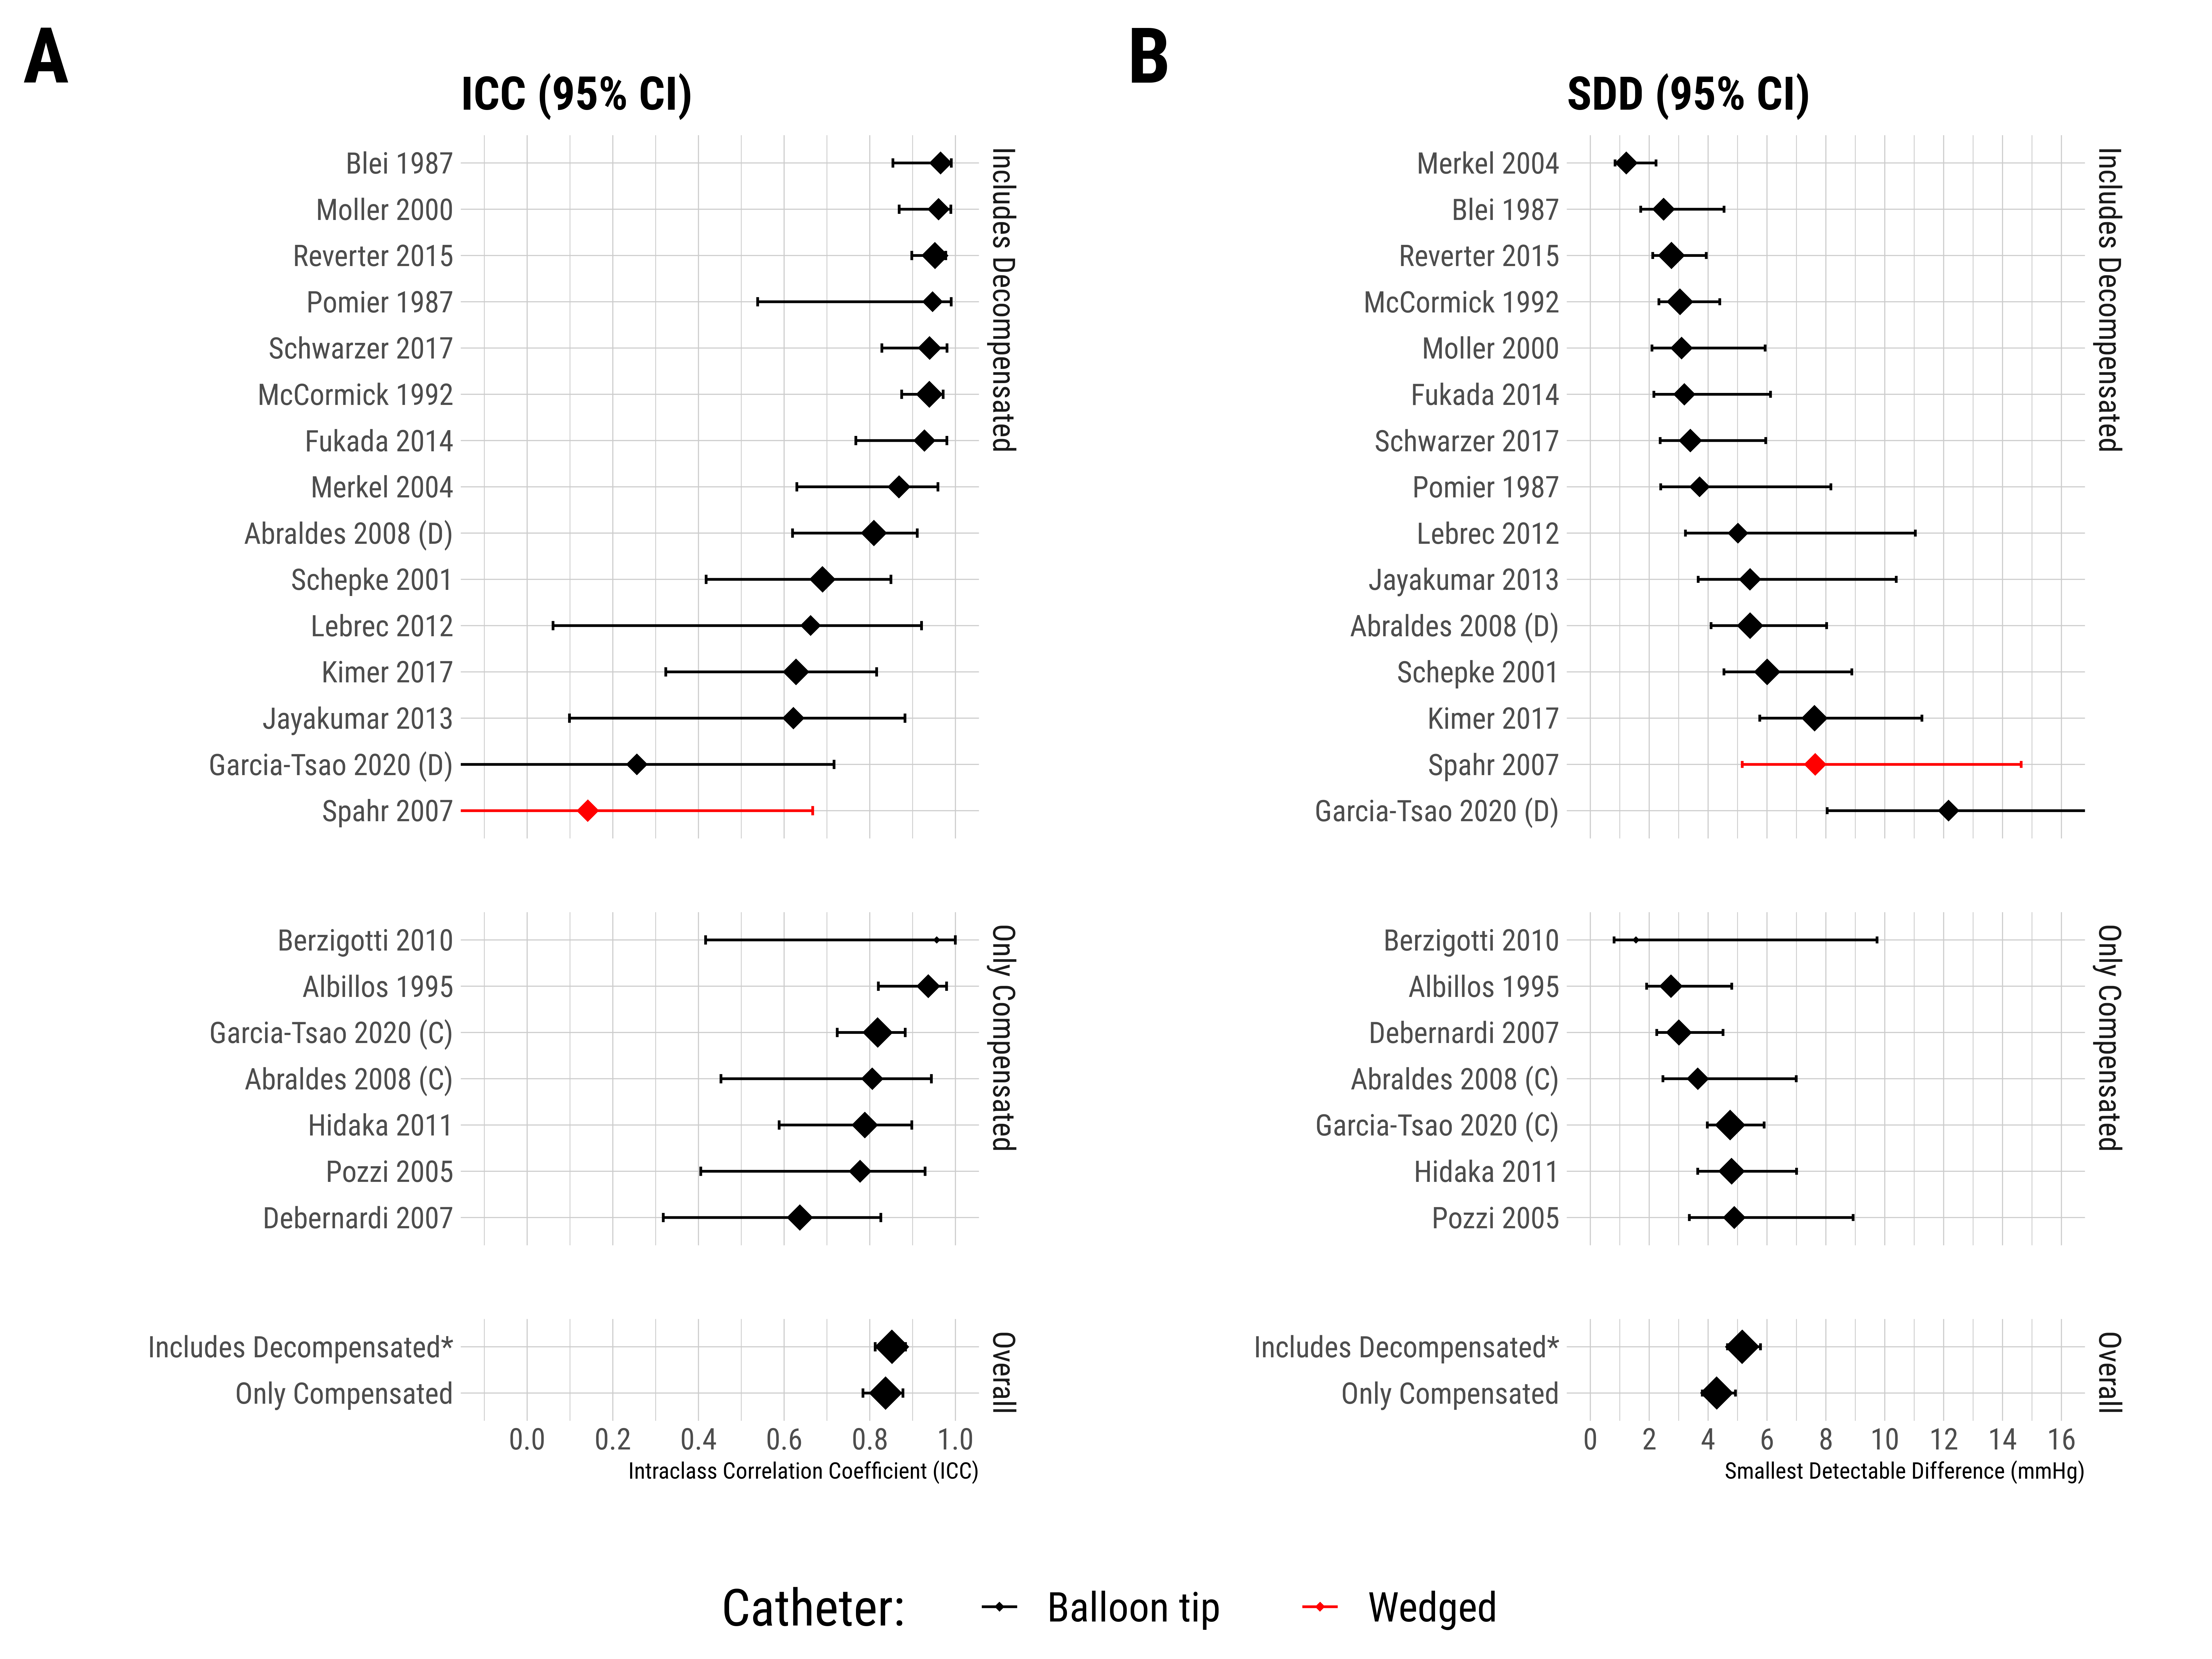
\includegraphics{figures/two_forest_row-1.png}

\hypertarget{are-they-different}{%
\subsection{Are they different}\label{are-they-different}}

To test the difference between the groups, we'll bootstrap the
difference. That means we take 1000 random samples from each group of
the same size with replacement, and calculate the difference to get the
null distribution. Then we compare the difference we see to the
bootstrap distribution.

\begin{Shaded}
\begin{Highlighting}[]
\NormalTok{trt\_compare }\OtherTok{\textless{}{-}}\NormalTok{ trt\_tidy }\SpecialCharTok{\%\textgreater{}\%} 
  \FunctionTok{filter}\NormalTok{(Description }\SpecialCharTok{!=} \StringTok{"Spahr. Octreotide"}\NormalTok{) }\SpecialCharTok{\%\textgreater{}\%}
  \FunctionTok{select}\NormalTok{(}\SpecialCharTok{{-}}\NormalTok{Study) }\SpecialCharTok{\%\textgreater{}\%}
  \FunctionTok{rename}\NormalTok{(}\AttributeTok{Study=}\NormalTok{ New\_Description) }\SpecialCharTok{\%\textgreater{}\%} 
  \FunctionTok{left\_join}\NormalTok{(trt\_studydemog) }\SpecialCharTok{\%\textgreater{}\%} 
  \FunctionTok{mutate}\NormalTok{(}\AttributeTok{decomp =} \FunctionTok{ifelse}\NormalTok{(Perc\_Decomp }\SpecialCharTok{\textgreater{}}\DecValTok{0}\NormalTok{ , }
                           \AttributeTok{yes=}\StringTok{"Includes Decompensated"}\NormalTok{,}
                           \AttributeTok{no =} \StringTok{"Only Compensated"}\NormalTok{)) }\SpecialCharTok{\%\textgreater{}\%}
  \FunctionTok{group\_by}\NormalTok{(decomp) }\SpecialCharTok{\%\textgreater{}\%} 
  \FunctionTok{nest}\NormalTok{()}
\end{Highlighting}
\end{Shaded}

\hypertarget{icc-1}{%
\subsubsection{ICC}\label{icc-1}}

\begin{Shaded}
\begin{Highlighting}[]
\NormalTok{bootstrap\_icc\_single }\OtherTok{\textless{}{-}} \ControlFlowTok{function}\NormalTok{(data) \{}
  
\NormalTok{  sample\_ids }\OtherTok{\textless{}{-}} \FunctionTok{unique}\NormalTok{(data}\SpecialCharTok{$}\StringTok{\textasciigrave{}}\AttributeTok{Serial number}\StringTok{\textasciigrave{}}\NormalTok{)}
\NormalTok{  ids }\OtherTok{\textless{}{-}} \FunctionTok{sample}\NormalTok{(sample\_ids, }\FunctionTok{length}\NormalTok{(sample\_ids), }\AttributeTok{replace=}\ConstantTok{TRUE}\NormalTok{)}
  
\NormalTok{  data\_nested }\OtherTok{\textless{}{-}}\NormalTok{ data }\SpecialCharTok{\%\textgreater{}\%} 
    \FunctionTok{select}\NormalTok{(}\StringTok{\textasciigrave{}}\AttributeTok{Serial number}\StringTok{\textasciigrave{}}\NormalTok{, MEASUREMENT, PP) }\SpecialCharTok{\%\textgreater{}\%} 
    \FunctionTok{nest\_by}\NormalTok{(}\StringTok{\textasciigrave{}}\AttributeTok{Serial number}\StringTok{\textasciigrave{}}\NormalTok{)}
  
\NormalTok{  boot\_sample }\OtherTok{\textless{}{-}} \FunctionTok{tibble}\NormalTok{(}
    \StringTok{\textasciigrave{}}\AttributeTok{Serial number}\StringTok{\textasciigrave{}} \OtherTok{=}\NormalTok{ ids}
\NormalTok{  ) }\SpecialCharTok{\%\textgreater{}\%} 
    \FunctionTok{left\_join}\NormalTok{(data\_nested, }\AttributeTok{by=}\StringTok{"Serial number"}\NormalTok{) }\SpecialCharTok{\%\textgreater{}\%} 
    \FunctionTok{select}\NormalTok{(}\SpecialCharTok{{-}}\StringTok{\textasciigrave{}}\AttributeTok{Serial number}\StringTok{\textasciigrave{}}\NormalTok{) }\SpecialCharTok{\%\textgreater{}\%} 
    \FunctionTok{mutate}\NormalTok{(}\AttributeTok{boot\_serial =} \DecValTok{1}\SpecialCharTok{:}\FunctionTok{n}\NormalTok{()) }\SpecialCharTok{\%\textgreater{}\%} 
    \FunctionTok{unnest}\NormalTok{(data) }\SpecialCharTok{\%\textgreater{}\%} 
\NormalTok{    relfeas}\SpecialCharTok{::}\FunctionTok{trt\_widify}\NormalTok{(}\StringTok{"PP"}\NormalTok{, }\StringTok{"boot\_serial"}\NormalTok{, }\StringTok{"MEASUREMENT"}\NormalTok{)}

\NormalTok{  boot\_icc }\OtherTok{\textless{}{-}} \FunctionTok{suppressMessages}\NormalTok{(}
    \FunctionTok{suppressWarnings}\NormalTok{(}
\NormalTok{      psych}\SpecialCharTok{::}\FunctionTok{ICC}\NormalTok{(boot\_sample[,}\FunctionTok{c}\NormalTok{(}\DecValTok{2}\NormalTok{,}\DecValTok{3}\NormalTok{)])}\SpecialCharTok{$}\NormalTok{results}\SpecialCharTok{$}\NormalTok{ICC[}\DecValTok{2}\NormalTok{] ) )}
  \FunctionTok{return}\NormalTok{(boot\_icc)}
\NormalTok{\}}

\NormalTok{bootstrap\_icc }\OtherTok{\textless{}{-}} \ControlFlowTok{function}\NormalTok{(n, data, }\AttributeTok{colname=}\ConstantTok{NULL}\NormalTok{) \{}
  
\NormalTok{  out }\OtherTok{\textless{}{-}} \FunctionTok{tibble}\NormalTok{(}
    \AttributeTok{n =} \DecValTok{1}\SpecialCharTok{:}\NormalTok{n}
\NormalTok{  ) }\SpecialCharTok{\%\textgreater{}\%} 
    \FunctionTok{mutate}\NormalTok{(}\AttributeTok{boot\_icc =} \FunctionTok{map\_dbl}\NormalTok{(n, }\SpecialCharTok{\textasciitilde{}}\FunctionTok{bootstrap\_icc\_single}\NormalTok{(data)))}
  
  \ControlFlowTok{if}\NormalTok{(}\SpecialCharTok{!}\FunctionTok{is.null}\NormalTok{(colname)) \{}
    \FunctionTok{colnames}\NormalTok{(out)[}\DecValTok{2}\NormalTok{] }\OtherTok{\textless{}{-}}\NormalTok{ colname}
\NormalTok{  \}}
  
  \FunctionTok{return}\NormalTok{(out)}
\NormalTok{\}}
\end{Highlighting}
\end{Shaded}

\begin{Shaded}
\begin{Highlighting}[]
\NormalTok{trt\_compare\_iccvals }\OtherTok{\textless{}{-}}\NormalTok{ trt\_compare }\SpecialCharTok{\%\textgreater{}\%} 
  \FunctionTok{mutate}\NormalTok{(}\AttributeTok{boot =} \FunctionTok{map2}\NormalTok{(data, decomp, }\SpecialCharTok{\textasciitilde{}}\FunctionTok{bootstrap\_icc}\NormalTok{(}\DecValTok{10000}\NormalTok{, .x))) }\SpecialCharTok{\%\textgreater{}\%} 
  \FunctionTok{select}\NormalTok{(}\SpecialCharTok{{-}}\NormalTok{data) }\SpecialCharTok{\%\textgreater{}\%} 
  \FunctionTok{unnest}\NormalTok{(boot)}
\end{Highlighting}
\end{Shaded}

\begin{Shaded}
\begin{Highlighting}[]
\NormalTok{trt\_compare\_icc }\OtherTok{\textless{}{-}}\NormalTok{ trt\_compare\_iccvals }\SpecialCharTok{\%\textgreater{}\%} 
  \FunctionTok{spread}\NormalTok{(decomp, boot\_icc) }\SpecialCharTok{\%\textgreater{}\%} 
  \FunctionTok{mutate}\NormalTok{(}\AttributeTok{dif =} \StringTok{\textasciigrave{}}\AttributeTok{Only Compensated}\StringTok{\textasciigrave{}} \SpecialCharTok{{-}} \StringTok{\textasciigrave{}}\AttributeTok{Includes Decompensated}\StringTok{\textasciigrave{}}\NormalTok{)}

\FunctionTok{quantile}\NormalTok{(trt\_compare\_icc}\SpecialCharTok{$}\NormalTok{dif, }\FunctionTok{c}\NormalTok{(}\FloatTok{0.025}\NormalTok{, }\FloatTok{0.5}\NormalTok{, }\FloatTok{0.975}\NormalTok{)) }\CommentTok{\# 95\% CI}
\end{Highlighting}
\end{Shaded}

\begin{verbatim}
##        2.5%         50%       97.5% 
## -0.09604300 -0.01736313  0.06649128
\end{verbatim}

\begin{Shaded}
\begin{Highlighting}[]
\DecValTok{1}\SpecialCharTok{{-}}\FunctionTok{sum}\NormalTok{(trt\_compare\_icc}\SpecialCharTok{$}\NormalTok{dif }\SpecialCharTok{\textgreater{}} \DecValTok{0}\NormalTok{)}\SpecialCharTok{/}\DecValTok{10000} \CommentTok{\# one{-}sided p value}
\end{Highlighting}
\end{Shaded}

\begin{verbatim}
## [1] 0.6645
\end{verbatim}

Not significant

\hypertarget{sdd-1}{%
\subsubsection{SDD}\label{sdd-1}}

\begin{Shaded}
\begin{Highlighting}[]
\NormalTok{bootstrap\_sdd\_single }\OtherTok{\textless{}{-}} \ControlFlowTok{function}\NormalTok{(data) \{}
  
\NormalTok{  sample\_ids }\OtherTok{\textless{}{-}} \FunctionTok{unique}\NormalTok{(data}\SpecialCharTok{$}\StringTok{\textasciigrave{}}\AttributeTok{Serial number}\StringTok{\textasciigrave{}}\NormalTok{)}
\NormalTok{  ids }\OtherTok{\textless{}{-}} \FunctionTok{sample}\NormalTok{(sample\_ids, }\FunctionTok{length}\NormalTok{(sample\_ids), }\AttributeTok{replace=}\ConstantTok{TRUE}\NormalTok{)}
  
\NormalTok{  data\_nested }\OtherTok{\textless{}{-}}\NormalTok{ data }\SpecialCharTok{\%\textgreater{}\%} 
    \FunctionTok{select}\NormalTok{(}\StringTok{\textasciigrave{}}\AttributeTok{Serial number}\StringTok{\textasciigrave{}}\NormalTok{, MEASUREMENT, PP) }\SpecialCharTok{\%\textgreater{}\%} 
    \FunctionTok{nest\_by}\NormalTok{(}\StringTok{\textasciigrave{}}\AttributeTok{Serial number}\StringTok{\textasciigrave{}}\NormalTok{)}
  
\NormalTok{  boot\_sample }\OtherTok{\textless{}{-}} \FunctionTok{tibble}\NormalTok{(}
    \StringTok{\textasciigrave{}}\AttributeTok{Serial number}\StringTok{\textasciigrave{}} \OtherTok{=}\NormalTok{ ids}
\NormalTok{  ) }\SpecialCharTok{\%\textgreater{}\%} 
    \FunctionTok{left\_join}\NormalTok{(data\_nested, }\AttributeTok{by=}\StringTok{"Serial number"}\NormalTok{) }\SpecialCharTok{\%\textgreater{}\%} 
    \FunctionTok{select}\NormalTok{(}\SpecialCharTok{{-}}\StringTok{\textasciigrave{}}\AttributeTok{Serial number}\StringTok{\textasciigrave{}}\NormalTok{) }\SpecialCharTok{\%\textgreater{}\%} 
    \FunctionTok{mutate}\NormalTok{(}\AttributeTok{boot\_serial =} \DecValTok{1}\SpecialCharTok{:}\FunctionTok{n}\NormalTok{()) }\SpecialCharTok{\%\textgreater{}\%} 
    \FunctionTok{unnest}\NormalTok{(data) }\SpecialCharTok{\%\textgreater{}\%} 
\NormalTok{    relfeas}\SpecialCharTok{::}\FunctionTok{trt\_widify}\NormalTok{(}\StringTok{"PP"}\NormalTok{, }\StringTok{"boot\_serial"}\NormalTok{, }\StringTok{"MEASUREMENT"}\NormalTok{)}

\NormalTok{  boot\_sdd }\OtherTok{\textless{}{-}} \FunctionTok{suppressMessages}\NormalTok{(}
    \FunctionTok{suppressWarnings}\NormalTok{(}
\NormalTok{      agRee}\SpecialCharTok{::}\FunctionTok{agree.sdd}\NormalTok{(}\FunctionTok{as.matrix}\NormalTok{(boot\_sample[,}\FunctionTok{c}\NormalTok{(}\DecValTok{2}\NormalTok{,}\DecValTok{3}\NormalTok{)]))}\SpecialCharTok{$}\NormalTok{value ) )}
  \FunctionTok{return}\NormalTok{(boot\_sdd)}
\NormalTok{\}}


\NormalTok{bootstrap\_sdd\_single }\OtherTok{\textless{}{-}} \ControlFlowTok{function}\NormalTok{(data) \{}
  
\NormalTok{  sample\_ids }\OtherTok{\textless{}{-}} \FunctionTok{unique}\NormalTok{(data}\SpecialCharTok{$}\StringTok{\textasciigrave{}}\AttributeTok{Serial number}\StringTok{\textasciigrave{}}\NormalTok{)}
\NormalTok{  ids }\OtherTok{\textless{}{-}} \FunctionTok{sample}\NormalTok{(sample\_ids, }\FunctionTok{length}\NormalTok{(sample\_ids), }\AttributeTok{replace=}\ConstantTok{TRUE}\NormalTok{)}
  
\NormalTok{  data\_nested }\OtherTok{\textless{}{-}}\NormalTok{ data }\SpecialCharTok{\%\textgreater{}\%} 
    \FunctionTok{select}\NormalTok{(}\StringTok{\textasciigrave{}}\AttributeTok{Serial number}\StringTok{\textasciigrave{}}\NormalTok{, MEASUREMENT, PP) }\SpecialCharTok{\%\textgreater{}\%} 
    \FunctionTok{nest\_by}\NormalTok{(}\StringTok{\textasciigrave{}}\AttributeTok{Serial number}\StringTok{\textasciigrave{}}\NormalTok{)}
  
\NormalTok{  boot\_sample }\OtherTok{\textless{}{-}} \FunctionTok{tibble}\NormalTok{(}
    \StringTok{\textasciigrave{}}\AttributeTok{Serial number}\StringTok{\textasciigrave{}} \OtherTok{=}\NormalTok{ ids}
\NormalTok{  ) }\SpecialCharTok{\%\textgreater{}\%} 
    \FunctionTok{left\_join}\NormalTok{(data\_nested, }\AttributeTok{by=}\StringTok{"Serial number"}\NormalTok{) }\SpecialCharTok{\%\textgreater{}\%} 
    \FunctionTok{select}\NormalTok{(}\SpecialCharTok{{-}}\StringTok{\textasciigrave{}}\AttributeTok{Serial number}\StringTok{\textasciigrave{}}\NormalTok{) }\SpecialCharTok{\%\textgreater{}\%} 
    \FunctionTok{mutate}\NormalTok{(}\AttributeTok{boot\_serial =} \DecValTok{1}\SpecialCharTok{:}\FunctionTok{n}\NormalTok{()) }\SpecialCharTok{\%\textgreater{}\%} 
    \FunctionTok{unnest}\NormalTok{(data) }\SpecialCharTok{\%\textgreater{}\%} 
\NormalTok{    relfeas}\SpecialCharTok{::}\FunctionTok{trt\_widify}\NormalTok{(}\StringTok{"PP"}\NormalTok{, }\StringTok{"boot\_serial"}\NormalTok{, }\StringTok{"MEASUREMENT"}\NormalTok{)}

\NormalTok{  boot\_sdd }\OtherTok{\textless{}{-}} \FunctionTok{suppressMessages}\NormalTok{(}
    \FunctionTok{suppressWarnings}\NormalTok{(}
\NormalTok{      agRee}\SpecialCharTok{::}\FunctionTok{agree.sdd}\NormalTok{(}\FunctionTok{as.matrix}\NormalTok{(boot\_sample[,}\FunctionTok{c}\NormalTok{(}\DecValTok{2}\NormalTok{,}\DecValTok{3}\NormalTok{)]))}\SpecialCharTok{$}\NormalTok{value ) )}
  \FunctionTok{return}\NormalTok{(boot\_sdd)}
\NormalTok{\}}

\NormalTok{bootstrap\_sdd }\OtherTok{\textless{}{-}} \ControlFlowTok{function}\NormalTok{(n, data, }\AttributeTok{colname=}\ConstantTok{NULL}\NormalTok{) \{}
  
\NormalTok{  out }\OtherTok{\textless{}{-}} \FunctionTok{tibble}\NormalTok{(}
    \AttributeTok{n =} \DecValTok{1}\SpecialCharTok{:}\NormalTok{n}
\NormalTok{  ) }\SpecialCharTok{\%\textgreater{}\%} 
    \FunctionTok{mutate}\NormalTok{(}\AttributeTok{boot\_sdd =} \FunctionTok{map\_dbl}\NormalTok{(n, }\SpecialCharTok{\textasciitilde{}}\FunctionTok{bootstrap\_sdd\_single}\NormalTok{(data)))}
  
  \ControlFlowTok{if}\NormalTok{(}\SpecialCharTok{!}\FunctionTok{is.null}\NormalTok{(colname)) \{}
    \FunctionTok{colnames}\NormalTok{(out)[}\DecValTok{2}\NormalTok{] }\OtherTok{\textless{}{-}}\NormalTok{ colname}
\NormalTok{  \}}
  
  \FunctionTok{return}\NormalTok{(out)}
\NormalTok{\}}

\CommentTok{\# bootstrap\_sdd\_single(trt\_compare$data[[1]])}
\CommentTok{\# bootstrap\_sdd(100, trt\_compare$data[[1]], "test")}
\end{Highlighting}
\end{Shaded}

And now we test

\begin{Shaded}
\begin{Highlighting}[]
\NormalTok{trt\_compare\_sddvals }\OtherTok{\textless{}{-}}\NormalTok{ trt\_compare }\SpecialCharTok{\%\textgreater{}\%} 
  \FunctionTok{mutate}\NormalTok{(}\AttributeTok{boot =} \FunctionTok{map2}\NormalTok{(data, decomp, }\SpecialCharTok{\textasciitilde{}}\FunctionTok{bootstrap\_sdd}\NormalTok{(}\DecValTok{10000}\NormalTok{, .x))) }\SpecialCharTok{\%\textgreater{}\%} 
  \FunctionTok{select}\NormalTok{(}\SpecialCharTok{{-}}\NormalTok{data) }\SpecialCharTok{\%\textgreater{}\%} 
  \FunctionTok{unnest}\NormalTok{(boot)}
\end{Highlighting}
\end{Shaded}

\begin{Shaded}
\begin{Highlighting}[]
\NormalTok{trt\_compare\_sdd }\OtherTok{\textless{}{-}}\NormalTok{ trt\_compare\_sddvals }\SpecialCharTok{\%\textgreater{}\%} 
  \FunctionTok{spread}\NormalTok{(decomp, boot\_sdd) }\SpecialCharTok{\%\textgreater{}\%} 
  \FunctionTok{mutate}\NormalTok{(}\AttributeTok{dif =} \StringTok{\textasciigrave{}}\AttributeTok{Includes Decompensated}\StringTok{\textasciigrave{}} \SpecialCharTok{{-}} \StringTok{\textasciigrave{}}\AttributeTok{Only Compensated}\StringTok{\textasciigrave{}}\NormalTok{)}

\FunctionTok{quantile}\NormalTok{(trt\_compare\_sdd}\SpecialCharTok{$}\NormalTok{dif, }\FunctionTok{c}\NormalTok{(}\FloatTok{0.025}\NormalTok{, }\FloatTok{0.5}\NormalTok{, }\FloatTok{0.975}\NormalTok{)) }\CommentTok{\# 95\% CI}
\end{Highlighting}
\end{Shaded}

\begin{verbatim}
##       2.5%        50%      97.5% 
## -0.2412147  0.8292606  2.0480528
\end{verbatim}

\begin{Shaded}
\begin{Highlighting}[]
\DecValTok{1}\SpecialCharTok{{-}}\FunctionTok{sum}\NormalTok{(trt\_compare\_sdd}\SpecialCharTok{$}\NormalTok{dif }\SpecialCharTok{\textgreater{}} \DecValTok{0}\NormalTok{)}\SpecialCharTok{/}\DecValTok{10000} \CommentTok{\# one{-}sided p value}
\end{Highlighting}
\end{Shaded}

\begin{verbatim}
## [1] 0.0678
\end{verbatim}

\hypertarget{sddm}{%
\subsubsection{SDDM}\label{sddm}}

Percentage SDD

\begin{Shaded}
\begin{Highlighting}[]
\NormalTok{bootstrap\_sddm\_single }\OtherTok{\textless{}{-}} \ControlFlowTok{function}\NormalTok{(data) \{}
  
\NormalTok{  sample\_ids }\OtherTok{\textless{}{-}} \FunctionTok{unique}\NormalTok{(data}\SpecialCharTok{$}\StringTok{\textasciigrave{}}\AttributeTok{Serial number}\StringTok{\textasciigrave{}}\NormalTok{)}
\NormalTok{  ids }\OtherTok{\textless{}{-}} \FunctionTok{sample}\NormalTok{(sample\_ids, }\FunctionTok{length}\NormalTok{(sample\_ids), }\AttributeTok{replace=}\ConstantTok{TRUE}\NormalTok{)}
  
\NormalTok{  data\_nested }\OtherTok{\textless{}{-}}\NormalTok{ data }\SpecialCharTok{\%\textgreater{}\%} 
    \FunctionTok{select}\NormalTok{(}\StringTok{\textasciigrave{}}\AttributeTok{Serial number}\StringTok{\textasciigrave{}}\NormalTok{, MEASUREMENT, PP) }\SpecialCharTok{\%\textgreater{}\%} 
    \FunctionTok{nest\_by}\NormalTok{(}\StringTok{\textasciigrave{}}\AttributeTok{Serial number}\StringTok{\textasciigrave{}}\NormalTok{)}
  
\NormalTok{  boot\_sample }\OtherTok{\textless{}{-}} \FunctionTok{tibble}\NormalTok{(}
    \StringTok{\textasciigrave{}}\AttributeTok{Serial number}\StringTok{\textasciigrave{}} \OtherTok{=}\NormalTok{ ids}
\NormalTok{  ) }\SpecialCharTok{\%\textgreater{}\%} 
    \FunctionTok{left\_join}\NormalTok{(data\_nested, }\AttributeTok{by=}\StringTok{"Serial number"}\NormalTok{) }\SpecialCharTok{\%\textgreater{}\%} 
    \FunctionTok{select}\NormalTok{(}\SpecialCharTok{{-}}\StringTok{\textasciigrave{}}\AttributeTok{Serial number}\StringTok{\textasciigrave{}}\NormalTok{) }\SpecialCharTok{\%\textgreater{}\%} 
    \FunctionTok{mutate}\NormalTok{(}\AttributeTok{boot\_serial =} \DecValTok{1}\SpecialCharTok{:}\FunctionTok{n}\NormalTok{()) }\SpecialCharTok{\%\textgreater{}\%} 
    \FunctionTok{unnest}\NormalTok{(data) }\SpecialCharTok{\%\textgreater{}\%} 
\NormalTok{    relfeas}\SpecialCharTok{::}\FunctionTok{trt\_widify}\NormalTok{(}\StringTok{"PP"}\NormalTok{, }\StringTok{"boot\_serial"}\NormalTok{, }\StringTok{"MEASUREMENT"}\NormalTok{)}

\NormalTok{  boot\_sddm }\OtherTok{\textless{}{-}} \FunctionTok{suppressMessages}\NormalTok{(}
    \FunctionTok{suppressWarnings}\NormalTok{(}
\NormalTok{      agRee}\SpecialCharTok{::}\FunctionTok{agree.sddm}\NormalTok{(}\FunctionTok{as.matrix}\NormalTok{(boot\_sample[,}\FunctionTok{c}\NormalTok{(}\DecValTok{2}\NormalTok{,}\DecValTok{3}\NormalTok{)]))}\SpecialCharTok{$}\NormalTok{value ) )}
  \FunctionTok{return}\NormalTok{(boot\_sddm)}
\NormalTok{\}}

\NormalTok{bootstrap\_sddm }\OtherTok{\textless{}{-}} \ControlFlowTok{function}\NormalTok{(n, data, }\AttributeTok{colname=}\ConstantTok{NULL}\NormalTok{) \{}
  
\NormalTok{  out }\OtherTok{\textless{}{-}} \FunctionTok{tibble}\NormalTok{(}
    \AttributeTok{n =} \DecValTok{1}\SpecialCharTok{:}\NormalTok{n}
\NormalTok{  ) }\SpecialCharTok{\%\textgreater{}\%} 
    \FunctionTok{mutate}\NormalTok{(}\AttributeTok{boot\_sddm =} \FunctionTok{map\_dbl}\NormalTok{(n, }\SpecialCharTok{\textasciitilde{}}\FunctionTok{bootstrap\_sddm\_single}\NormalTok{(data)))}
  
  \ControlFlowTok{if}\NormalTok{(}\SpecialCharTok{!}\FunctionTok{is.null}\NormalTok{(colname)) \{}
    \FunctionTok{colnames}\NormalTok{(out)[}\DecValTok{2}\NormalTok{] }\OtherTok{\textless{}{-}}\NormalTok{ colname}
\NormalTok{  \}}
  
  \FunctionTok{return}\NormalTok{(out)}
\NormalTok{\}}

\CommentTok{\# bootstrap\_sddm\_single(trt\_compare$data[[1]])}
\CommentTok{\# bootstrap\_sddm(100, trt\_compare$data[[1]], "test")}
\end{Highlighting}
\end{Shaded}

And now we test

\begin{Shaded}
\begin{Highlighting}[]
\NormalTok{trt\_compare\_sddmvals }\OtherTok{\textless{}{-}}\NormalTok{ trt\_compare }\SpecialCharTok{\%\textgreater{}\%} 
  \FunctionTok{mutate}\NormalTok{(}\AttributeTok{boot =} \FunctionTok{map2}\NormalTok{(data, decomp, }\SpecialCharTok{\textasciitilde{}}\FunctionTok{bootstrap\_sddm}\NormalTok{(}\DecValTok{10000}\NormalTok{, .x))) }\SpecialCharTok{\%\textgreater{}\%} 
  \FunctionTok{select}\NormalTok{(}\SpecialCharTok{{-}}\NormalTok{data) }\SpecialCharTok{\%\textgreater{}\%} 
  \FunctionTok{unnest}\NormalTok{(boot)}
\end{Highlighting}
\end{Shaded}

\begin{Shaded}
\begin{Highlighting}[]
\NormalTok{trt\_compare\_sddm }\OtherTok{\textless{}{-}}\NormalTok{ trt\_compare\_sddmvals }\SpecialCharTok{\%\textgreater{}\%} 
  \FunctionTok{spread}\NormalTok{(decomp, boot\_sddm) }\SpecialCharTok{\%\textgreater{}\%} 
  \FunctionTok{mutate}\NormalTok{(}\AttributeTok{dif =} \StringTok{\textasciigrave{}}\AttributeTok{Includes Decompensated}\StringTok{\textasciigrave{}} \SpecialCharTok{{-}} \StringTok{\textasciigrave{}}\AttributeTok{Only Compensated}\StringTok{\textasciigrave{}}\NormalTok{)}

\FunctionTok{quantile}\NormalTok{(trt\_compare\_sddm}\SpecialCharTok{$}\NormalTok{dif, }\FunctionTok{c}\NormalTok{(}\FloatTok{0.025}\NormalTok{, }\FloatTok{0.5}\NormalTok{, }\FloatTok{0.975}\NormalTok{)) }\CommentTok{\# 95\% CI}
\end{Highlighting}
\end{Shaded}

\begin{verbatim}
##        2.5%         50%       97.5% 
## -0.03102582  0.03489179  0.10583268
\end{verbatim}

\begin{Shaded}
\begin{Highlighting}[]
\DecValTok{1}\SpecialCharTok{{-}}\FunctionTok{sum}\NormalTok{(trt\_compare\_sddm}\SpecialCharTok{$}\NormalTok{dif }\SpecialCharTok{\textgreater{}} \DecValTok{0}\NormalTok{)}\SpecialCharTok{/}\DecValTok{10000} \CommentTok{\# one{-}sided p value}
\end{Highlighting}
\end{Shaded}

\begin{verbatim}
## [1] 0.1557
\end{verbatim}

\hypertarget{causes-of-differences}{%
\section{Causes of differences}\label{causes-of-differences}}

Here, we perform an exploratory analysis of which factors may contribute
to differences

\begin{Shaded}
\begin{Highlighting}[]
\NormalTok{trt\_wide }\OtherTok{\textless{}{-}}\NormalTok{ trt\_tidy }\SpecialCharTok{\%\textgreater{}\%} 
  \FunctionTok{select}\NormalTok{(}\SpecialCharTok{{-}}\NormalTok{Study) }\SpecialCharTok{\%\textgreater{}\%}
  \FunctionTok{rename}\NormalTok{(}\AttributeTok{Study=}\NormalTok{ New\_Description) }\SpecialCharTok{\%\textgreater{}\%} 
  \FunctionTok{spread}\NormalTok{(MEASUREMENT, PP) }\SpecialCharTok{\%\textgreater{}\%} 
  \FunctionTok{rename}\NormalTok{(}\AttributeTok{Meas1 =} \StringTok{\textasciigrave{}}\AttributeTok{1}\StringTok{\textasciigrave{}}\NormalTok{,}
         \AttributeTok{Meas2 =} \StringTok{\textasciigrave{}}\AttributeTok{2}\StringTok{\textasciigrave{}}\NormalTok{) }\SpecialCharTok{\%\textgreater{}\%} 
  \FunctionTok{mutate}\NormalTok{(}\AttributeTok{change =}\NormalTok{ Meas2 }\SpecialCharTok{{-}}\NormalTok{ Meas1,}
         \AttributeTok{abschange=}\FunctionTok{abs}\NormalTok{(change),}
         \AttributeTok{meanval =}\NormalTok{ (Meas1 }\SpecialCharTok{+}\NormalTok{ Meas2)}\SpecialCharTok{/}\DecValTok{2}\NormalTok{) }\SpecialCharTok{\%\textgreater{}\%} 
  \FunctionTok{left\_join}\NormalTok{(studynames) }\SpecialCharTok{\%\textgreater{}\%} 
  \FunctionTok{left\_join}\NormalTok{(trt\_studydemog) }\SpecialCharTok{\%\textgreater{}\%} 
  \FunctionTok{mutate}\NormalTok{(}\AttributeTok{Description =} \FunctionTok{as.factor}\NormalTok{(Description)) }\SpecialCharTok{\%\textgreater{}\%} 
  \FunctionTok{filter}\NormalTok{(Description }\SpecialCharTok{!=} \StringTok{"Spahr. Octreotide"}\NormalTok{) }\SpecialCharTok{\%\textgreater{}\%} 
  \FunctionTok{mutate}\NormalTok{(}\AttributeTok{decomp =} \FunctionTok{ifelse}\NormalTok{(Perc\_Decomp }\SpecialCharTok{==} \DecValTok{0}\NormalTok{,}
                         \StringTok{"Only Compensated"}\NormalTok{,}
                         \StringTok{"Includes Decompensated"}\NormalTok{))}


\NormalTok{trt\_wide\_c }\OtherTok{\textless{}{-}}\NormalTok{ trt\_wide }\SpecialCharTok{\%\textgreater{}\%} 
  \FunctionTok{filter}\NormalTok{(Perc\_Decomp }\SpecialCharTok{==} \DecValTok{0}\NormalTok{)}

\NormalTok{trt\_wide\_dc }\OtherTok{\textless{}{-}}\NormalTok{ trt\_wide }\SpecialCharTok{\%\textgreater{}\%} 
  \FunctionTok{filter}\NormalTok{(Perc\_Decomp }\SpecialCharTok{\textgreater{}} \DecValTok{0}\NormalTok{)}
\end{Highlighting}
\end{Shaded}

\hypertarget{skewness}{%
\subsection{Skewness}\label{skewness}}

\hypertarget{absolute-1}{%
\subsubsection{Absolute}\label{absolute-1}}

Let's just visualise our distribution.

\begin{Shaded}
\begin{Highlighting}[]
\FunctionTok{ggplot}\NormalTok{(trt\_wide, }\FunctionTok{aes}\NormalTok{(}\AttributeTok{x=}\NormalTok{abschange)) }\SpecialCharTok{+}
  \FunctionTok{geom\_density}\NormalTok{(}\AttributeTok{fill=}\StringTok{"black"}\NormalTok{,}\AttributeTok{alpha=}\FloatTok{0.5}\NormalTok{)}
\end{Highlighting}
\end{Shaded}

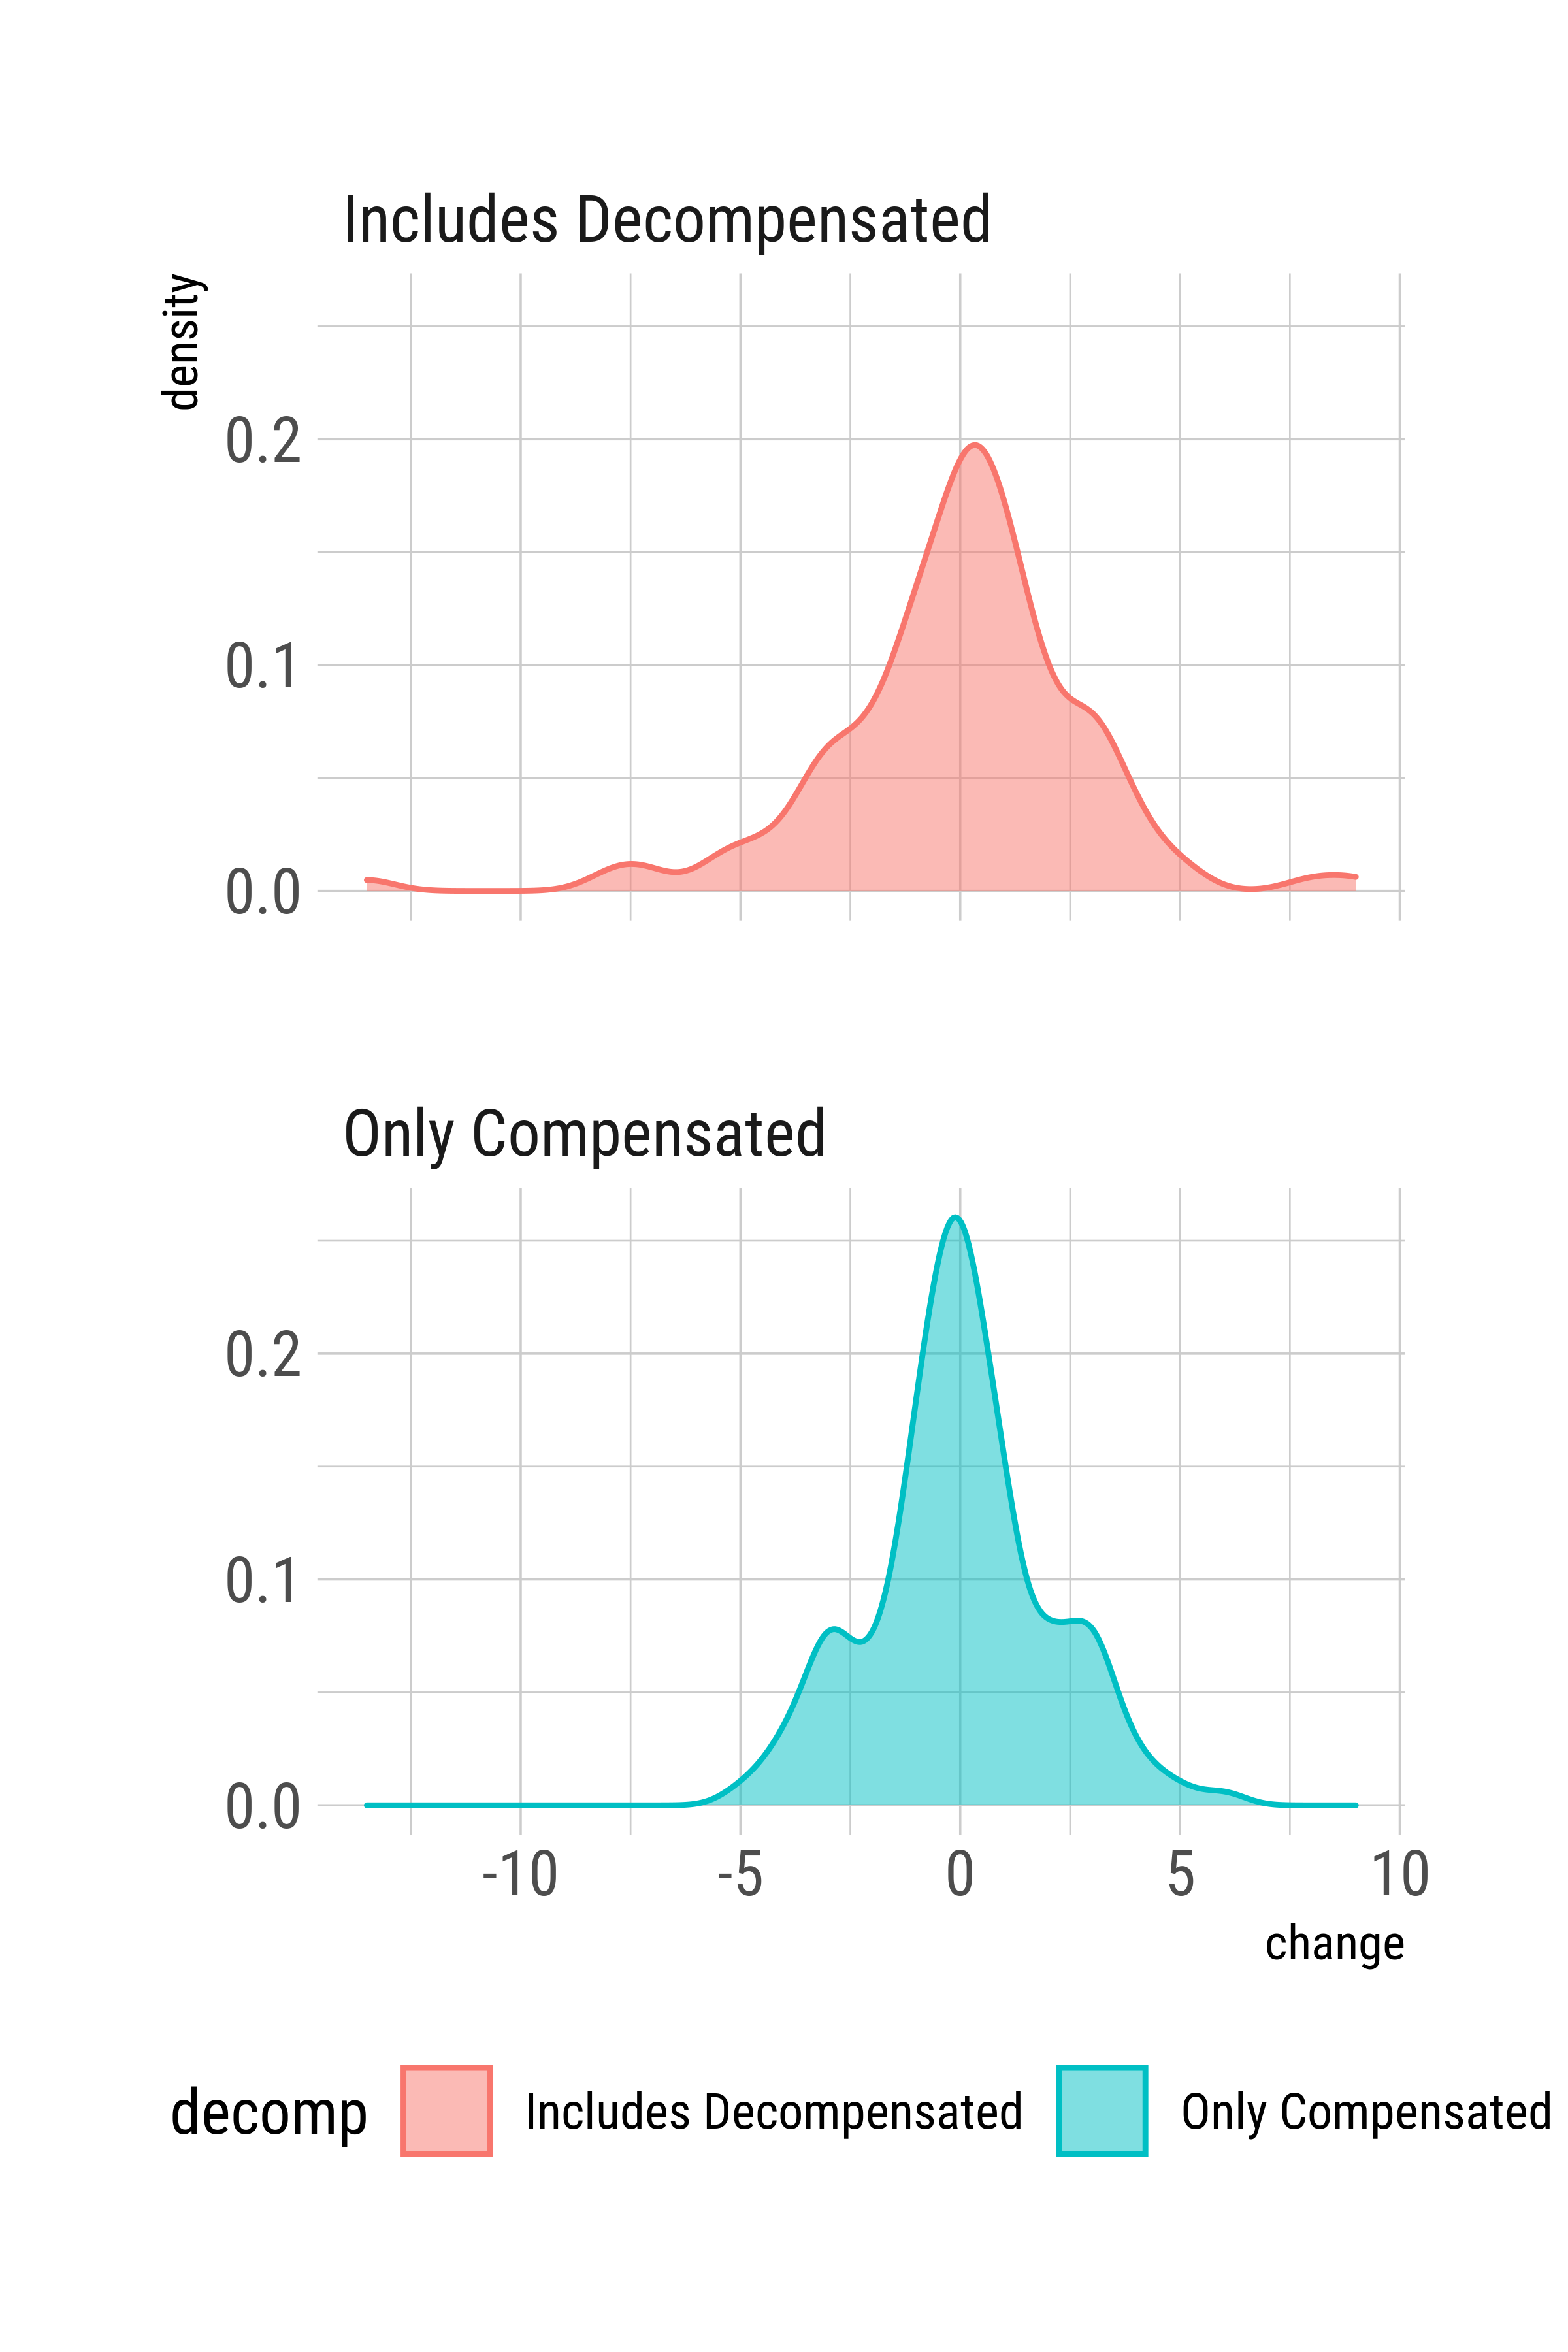
\includegraphics{figures/unnamed-chunk-25-1.png} And between groups

\begin{Shaded}
\begin{Highlighting}[]
\FunctionTok{ggplot}\NormalTok{(trt\_wide, }\FunctionTok{aes}\NormalTok{(}\AttributeTok{x=}\NormalTok{abschange)) }\SpecialCharTok{+}
  \FunctionTok{geom\_density}\NormalTok{(}\FunctionTok{aes}\NormalTok{(}\AttributeTok{colour=}\NormalTok{decomp, }\AttributeTok{fill=}\NormalTok{decomp),}\AttributeTok{alpha=}\FloatTok{0.5}\NormalTok{) }\SpecialCharTok{+}
  \FunctionTok{facet\_wrap}\NormalTok{(decomp}\SpecialCharTok{\textasciitilde{}}\NormalTok{., }\AttributeTok{nrow=}\DecValTok{2}\NormalTok{) }\SpecialCharTok{+}
  \FunctionTok{theme}\NormalTok{(}\AttributeTok{legend.position=}\StringTok{"bottom"}\NormalTok{)}
\end{Highlighting}
\end{Shaded}

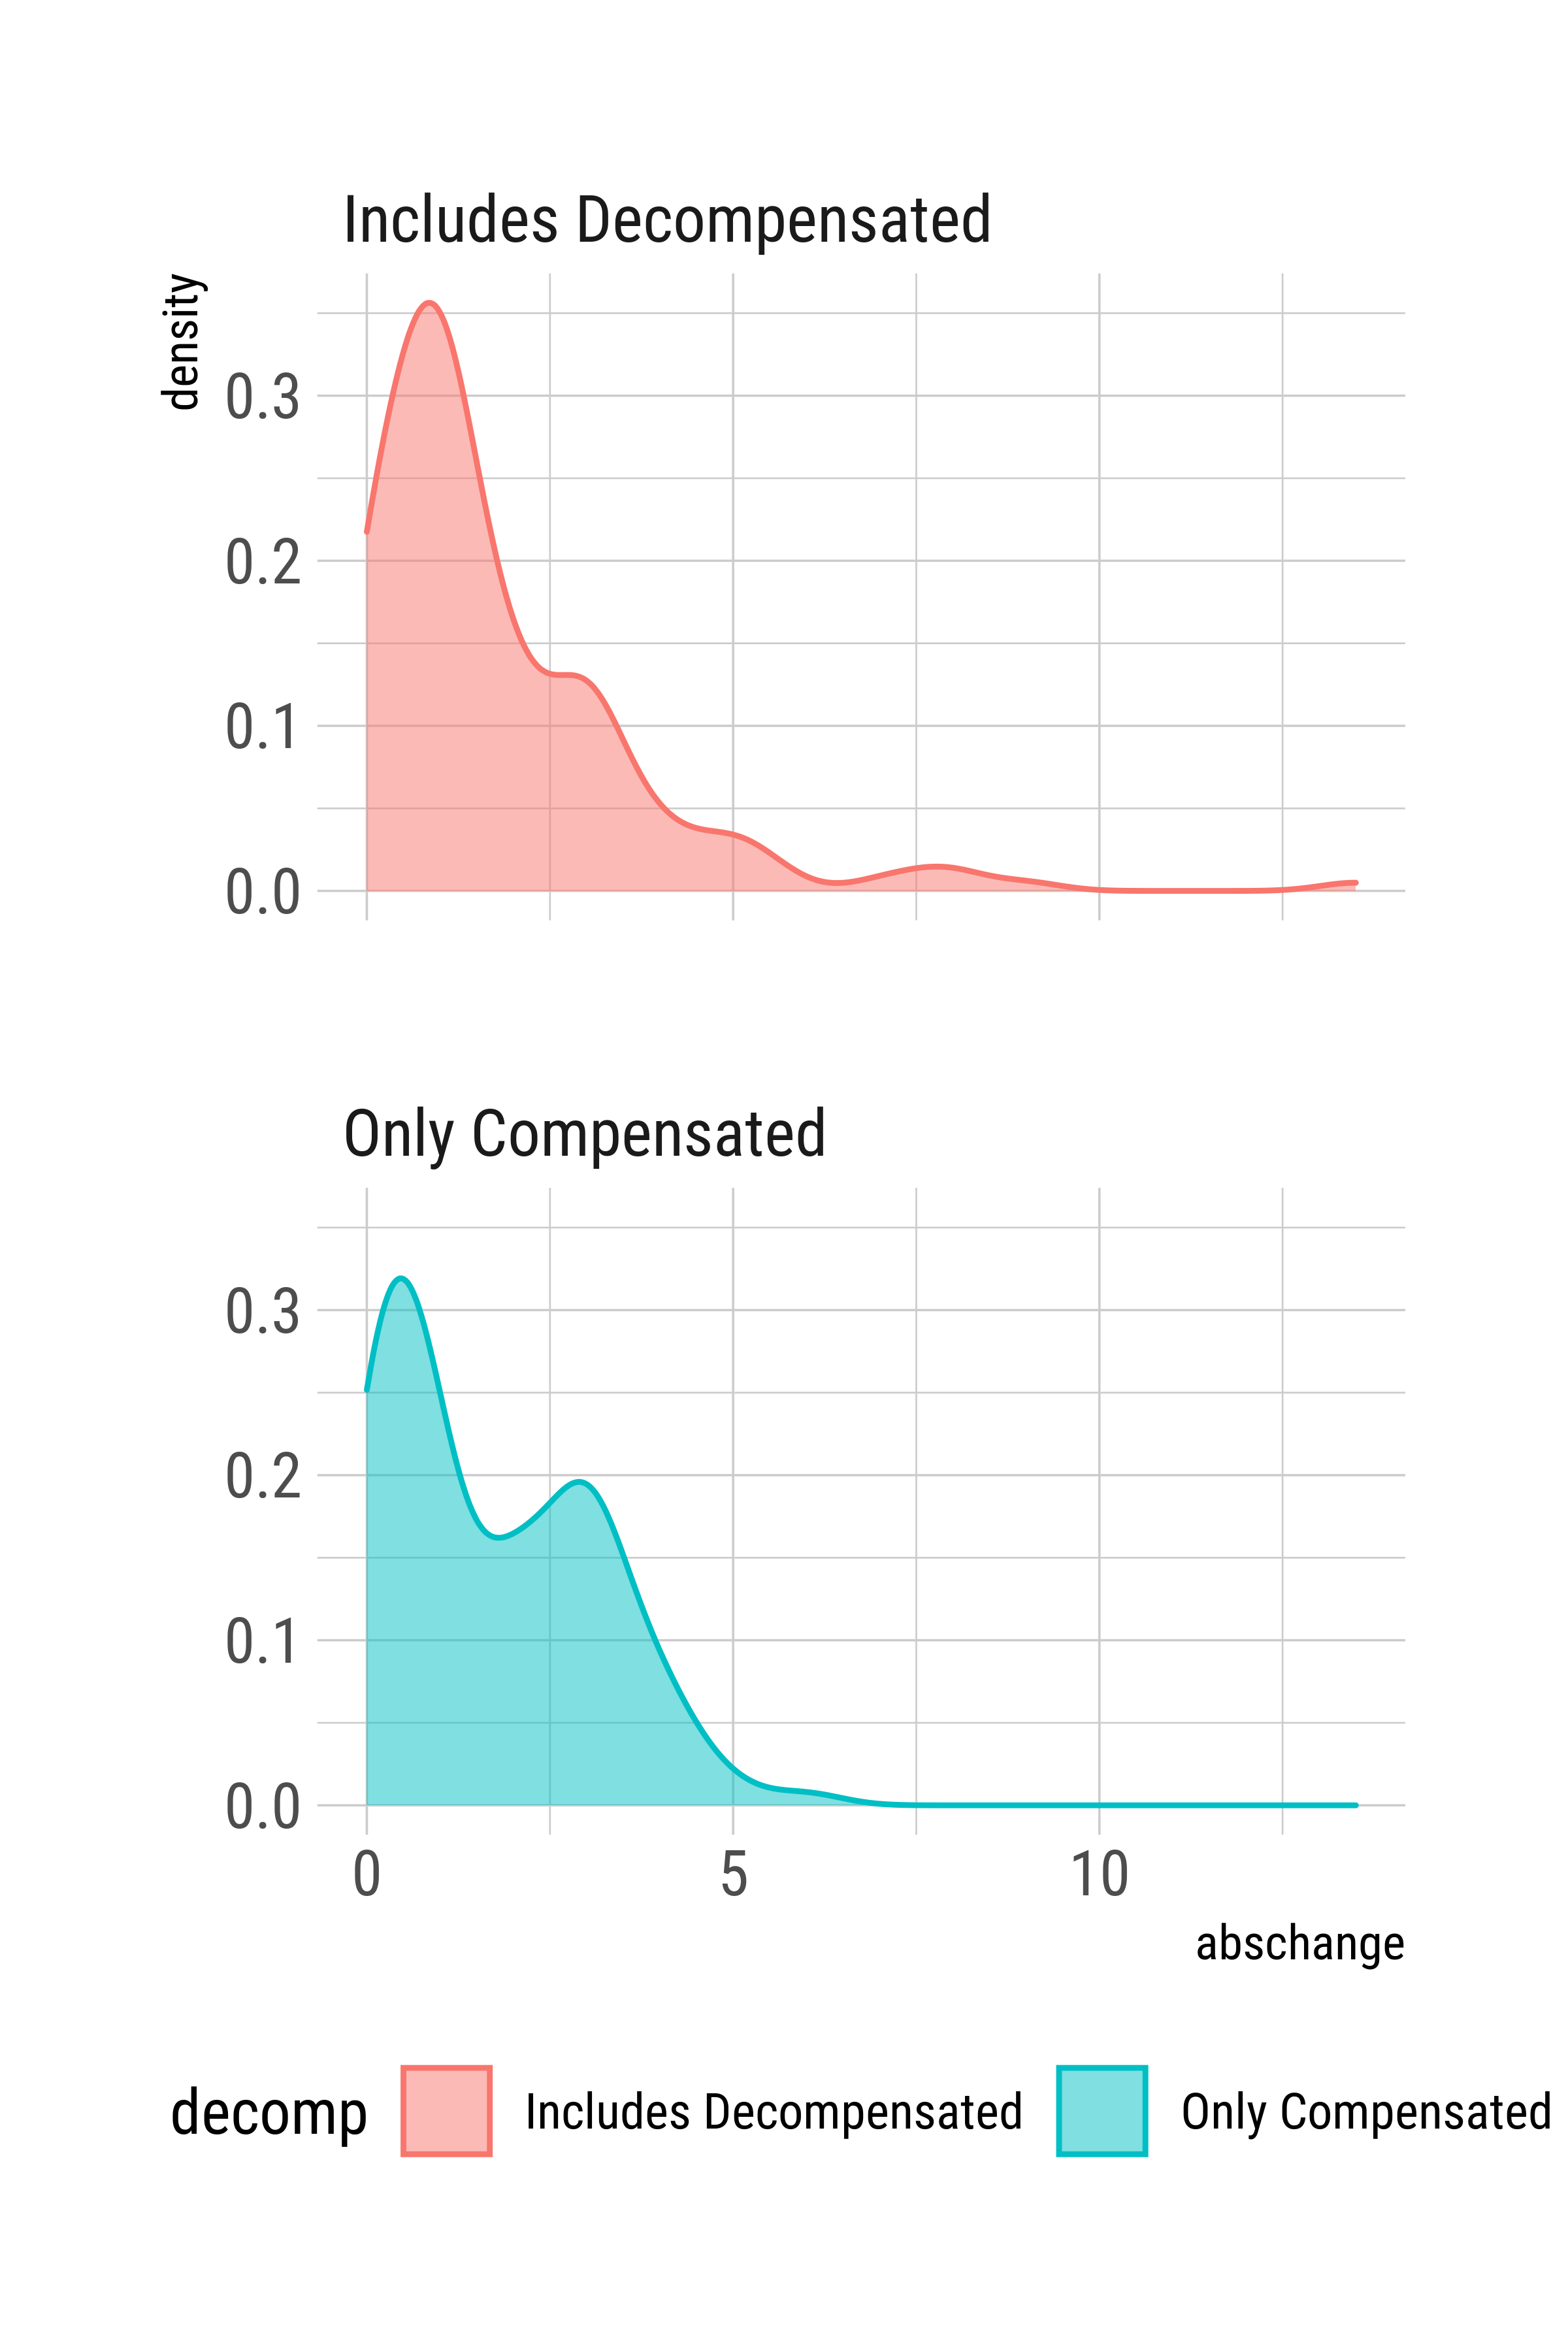
\includegraphics{figures/unnamed-chunk-26-1.png}

And let's get some values for that too

\begin{Shaded}
\begin{Highlighting}[]
\NormalTok{psych}\SpecialCharTok{::}\FunctionTok{describe}\NormalTok{(trt\_wide}\SpecialCharTok{$}\NormalTok{abschange)}
\end{Highlighting}
\end{Shaded}

\begin{verbatim}
##    vars   n mean   sd median trimmed  mad min  max range skew kurtosis  se
## X1    1 281 1.74 1.74      1     1.5 1.48   0 13.5  13.5 2.14     8.37 0.1
\end{verbatim}

\begin{Shaded}
\begin{Highlighting}[]
\NormalTok{psych}\SpecialCharTok{::}\FunctionTok{describeBy}\NormalTok{(trt\_wide}\SpecialCharTok{$}\NormalTok{abschange, }\AttributeTok{group=}\NormalTok{trt\_wide}\SpecialCharTok{$}\NormalTok{decomp)}
\end{Highlighting}
\end{Shaded}

\begin{verbatim}
## 
##  Descriptive statistics by group 
## group: Includes Decompensated
##    vars   n mean   sd median trimmed  mad min  max range skew kurtosis   se
## X1    1 166 1.79 1.94      1    1.46 1.11   0 13.5  13.5 2.45     8.89 0.15
## ------------------------------------------------------------ 
## group: Only Compensated
##    vars   n mean   sd median trimmed  mad min max range skew kurtosis   se
## X1    1 115 1.67 1.42      1    1.56 1.48   0   6     6 0.57    -0.64 0.13
\end{verbatim}

\hypertarget{signed}{%
\subsubsection{Signed}\label{signed}}

Let's just visualise our overall distribution.

\begin{Shaded}
\begin{Highlighting}[]
\FunctionTok{ggplot}\NormalTok{(trt\_wide, }\FunctionTok{aes}\NormalTok{(}\AttributeTok{x=}\NormalTok{change)) }\SpecialCharTok{+}
  \FunctionTok{geom\_density}\NormalTok{(}\AttributeTok{fill=}\StringTok{"black"}\NormalTok{,}\AttributeTok{alpha=}\FloatTok{0.5}\NormalTok{)}
\end{Highlighting}
\end{Shaded}

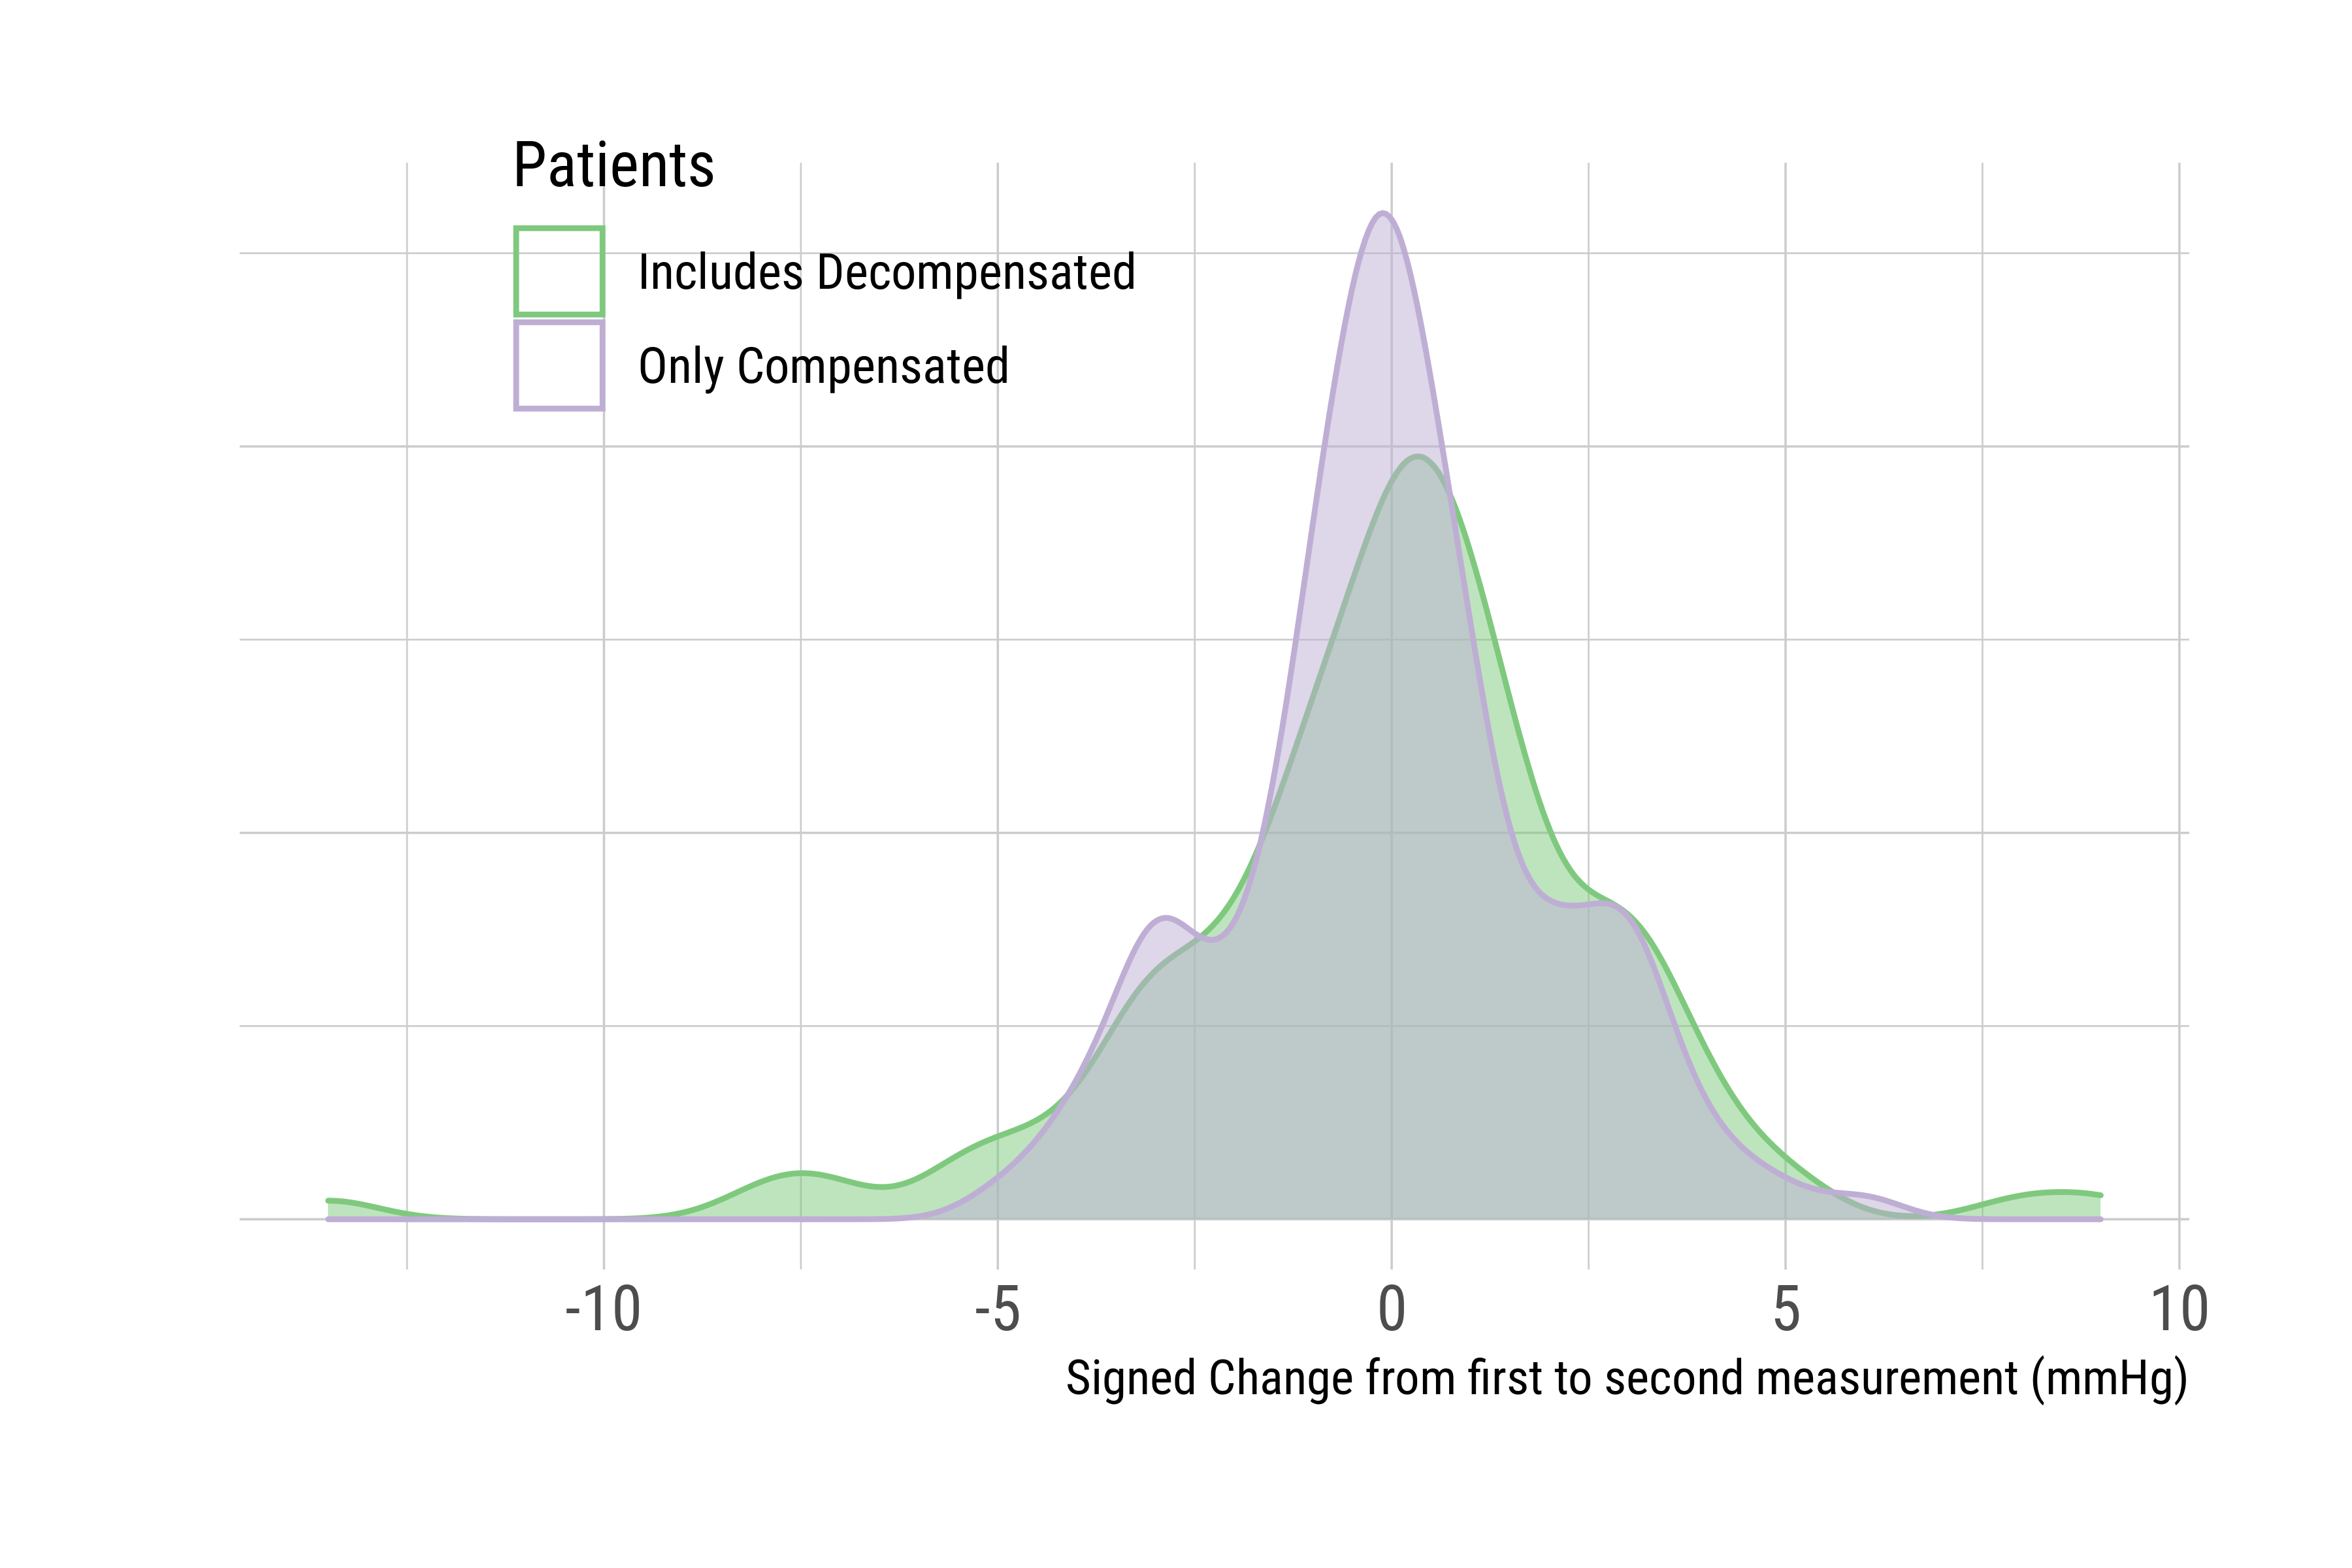
\includegraphics{figures/unnamed-chunk-28-1.png} \ldots{} and by group

\begin{Shaded}
\begin{Highlighting}[]
\FunctionTok{ggplot}\NormalTok{(trt\_wide, }\FunctionTok{aes}\NormalTok{(}\AttributeTok{x=}\NormalTok{change)) }\SpecialCharTok{+}
  \FunctionTok{geom\_density}\NormalTok{(}\FunctionTok{aes}\NormalTok{(}\AttributeTok{colour=}\NormalTok{decomp, }\AttributeTok{fill=}\NormalTok{decomp),}\AttributeTok{alpha=}\FloatTok{0.5}\NormalTok{) }\SpecialCharTok{+}
  \FunctionTok{facet\_wrap}\NormalTok{(decomp}\SpecialCharTok{\textasciitilde{}}\NormalTok{., }\AttributeTok{nrow=}\DecValTok{2}\NormalTok{) }\SpecialCharTok{+}
  \FunctionTok{theme}\NormalTok{(}\AttributeTok{legend.position=}\StringTok{"bottom"}\NormalTok{)}
\end{Highlighting}
\end{Shaded}

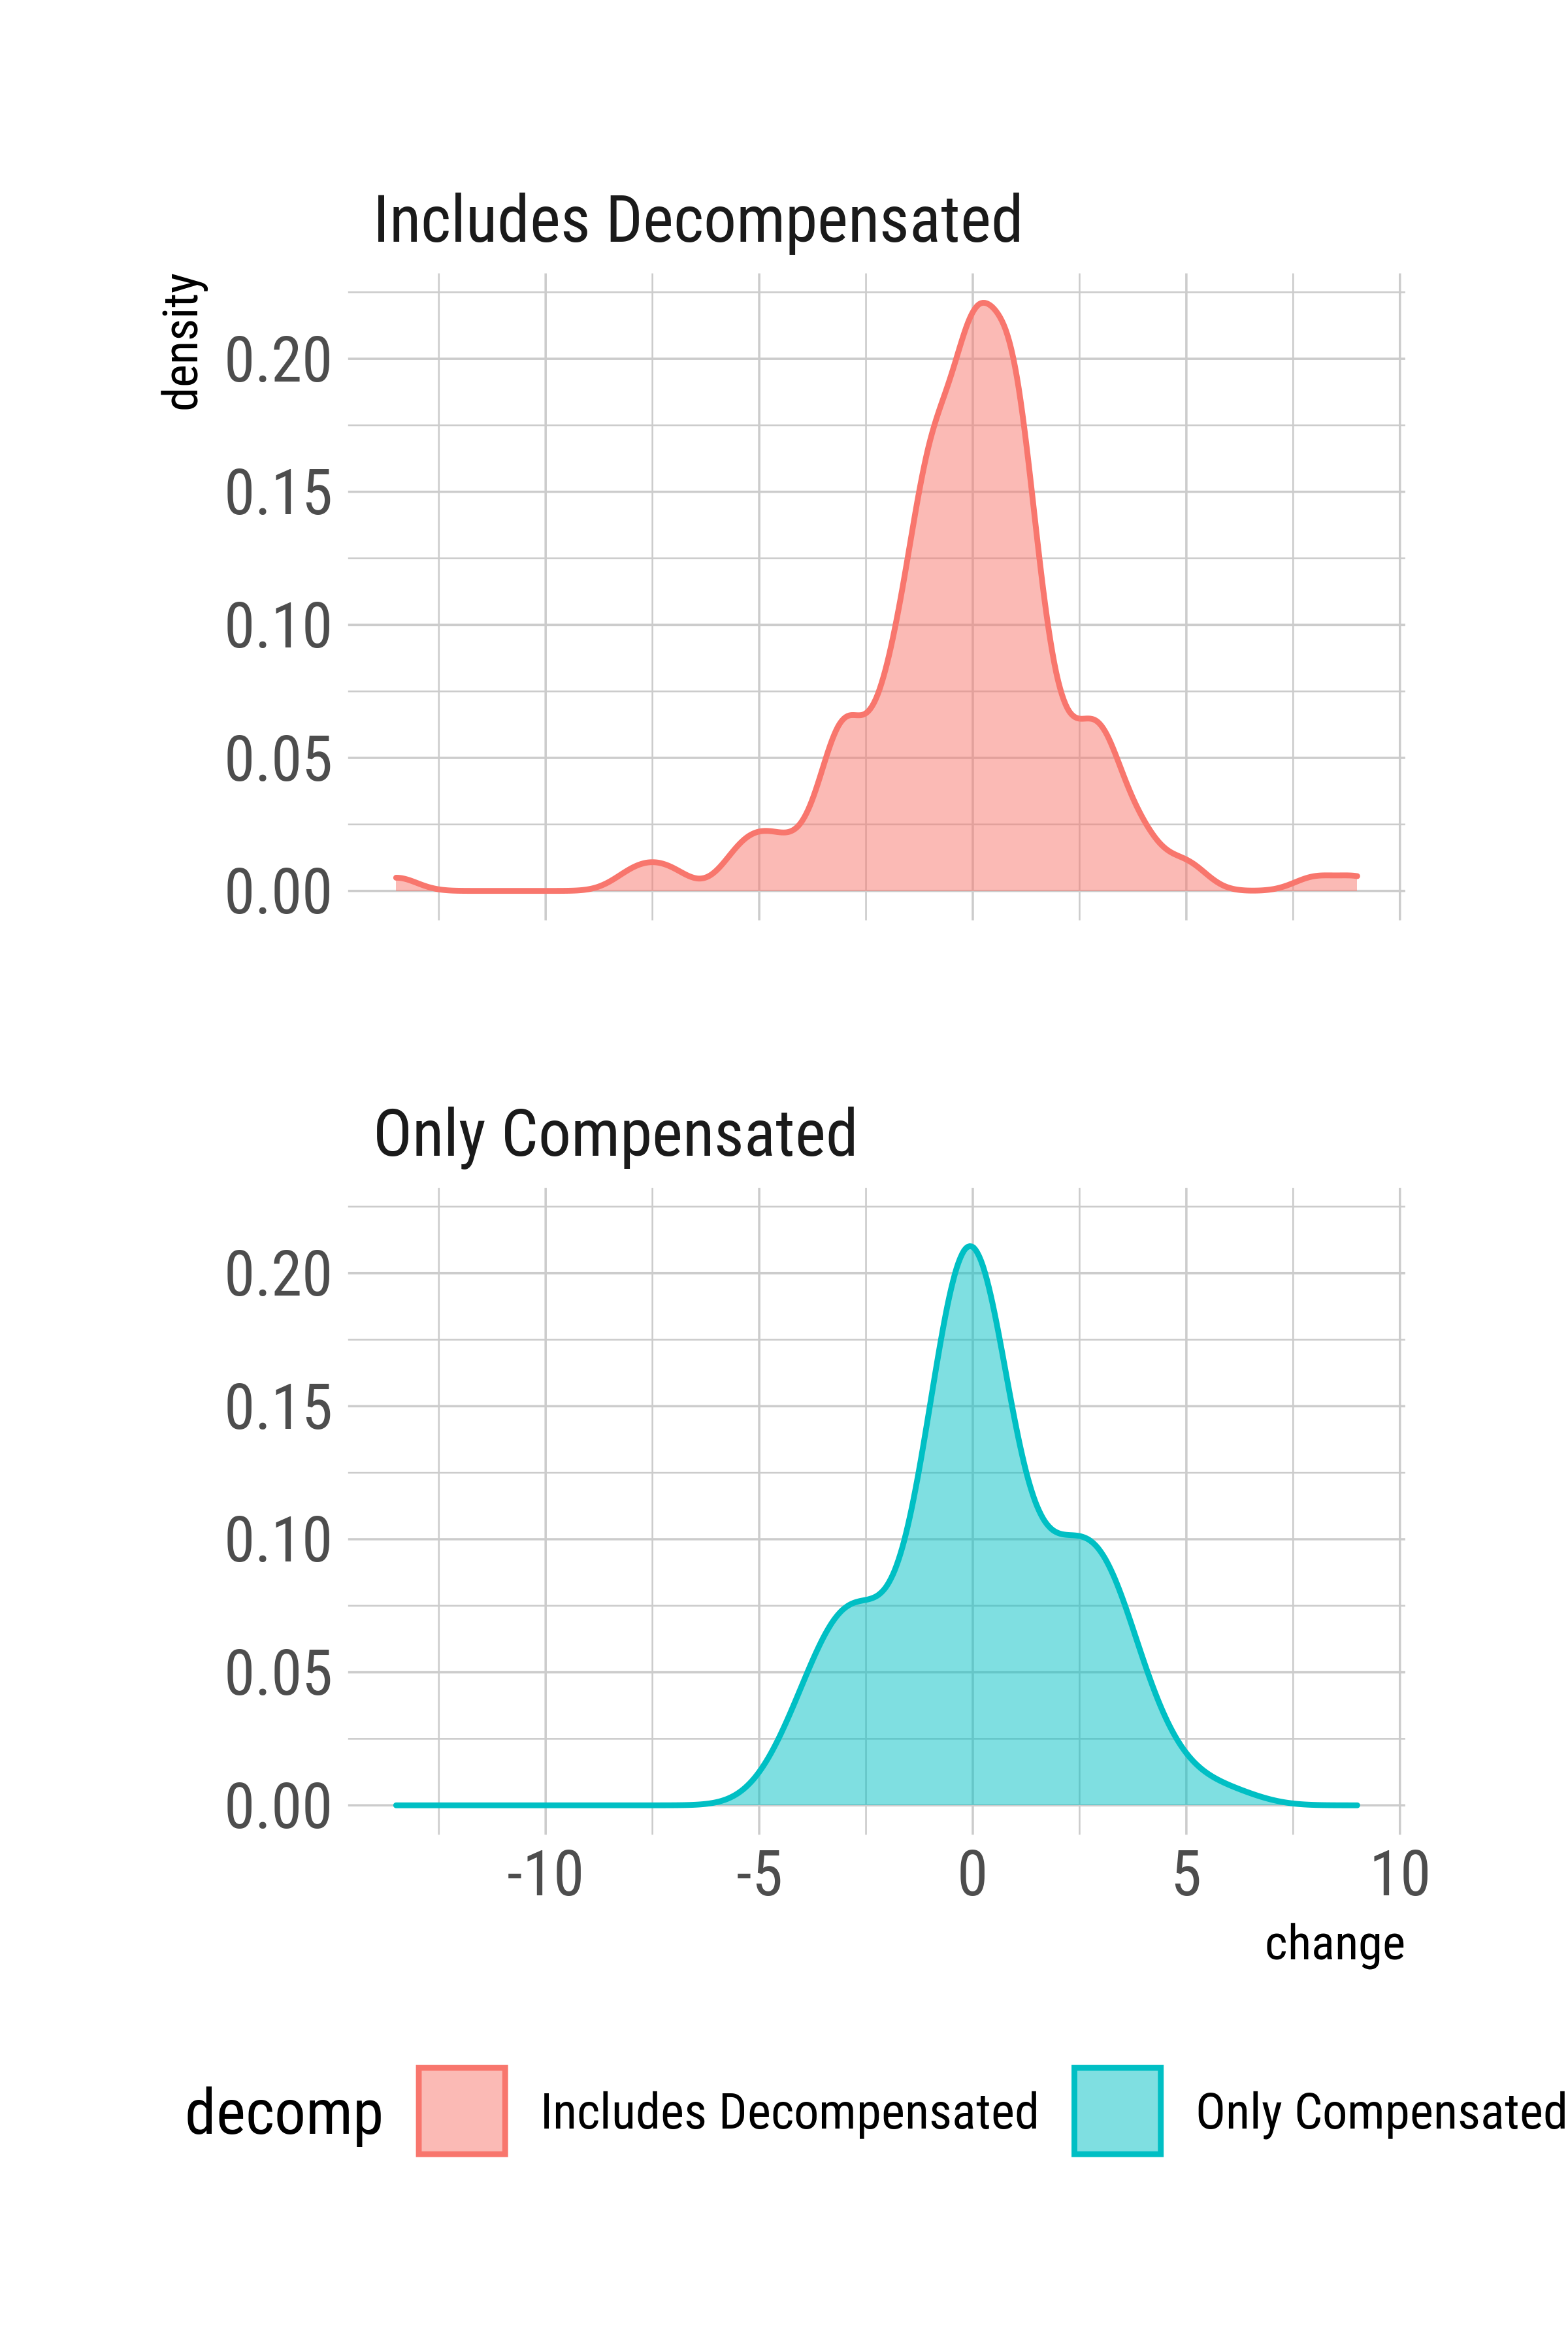
\includegraphics{figures/unnamed-chunk-29-1.png}

For signed differences, let's assess whether they differ from zero.

\begin{Shaded}
\begin{Highlighting}[]
\FunctionTok{summary}\NormalTok{(}\FunctionTok{lmer}\NormalTok{(change }\SpecialCharTok{\textasciitilde{}} \DecValTok{1} \SpecialCharTok{+}\NormalTok{ (}\DecValTok{1}\SpecialCharTok{|}\NormalTok{Study), }\AttributeTok{data=}\NormalTok{trt\_wide))}
\end{Highlighting}
\end{Shaded}

\begin{verbatim}
## Linear mixed model fit by REML. t-tests use Satterthwaite's method [
## lmerModLmerTest]
## Formula: change ~ 1 + (1 | Study)
##    Data: trt_wide
## 
## REML criterion at convergence: 1304.2
## 
## Scaled residuals: 
##     Min      1Q  Median      3Q     Max 
## -5.1470 -0.4712 -0.0170  0.5292  3.7968 
## 
## Random effects:
##  Groups   Name        Variance Std.Dev.
##  Study    (Intercept) 0.2793   0.5285  
##  Residual             5.8542   2.4195  
## Number of obs: 281, groups:  Study, 21
## 
## Fixed effects:
##             Estimate Std. Error       df t value Pr(>|t|)
## (Intercept) -0.03655    0.19379  9.51195  -0.189    0.854
\end{verbatim}

\begin{Shaded}
\begin{Highlighting}[]
\FunctionTok{summary}\NormalTok{(}\FunctionTok{lmer}\NormalTok{(change }\SpecialCharTok{\textasciitilde{}} \DecValTok{1} \SpecialCharTok{+}\NormalTok{ (}\DecValTok{1}\SpecialCharTok{|}\NormalTok{Study), }\AttributeTok{data=}\NormalTok{trt\_wide\_c))}
\end{Highlighting}
\end{Shaded}

\begin{verbatim}
## Linear mixed model fit by REML. t-tests use Satterthwaite's method [
## lmerModLmerTest]
## Formula: change ~ 1 + (1 | Study)
##    Data: trt_wide_c
## 
## REML criterion at convergence: 506.5
## 
## Scaled residuals: 
##     Min      1Q  Median      3Q     Max 
## -2.1852 -0.5692 -0.1075  0.7360  2.6627 
## 
## Random effects:
##  Groups   Name        Variance Std.Dev.
##  Study    (Intercept) 0.1414   0.3761  
##  Residual             4.6911   2.1659  
## Number of obs: 115, groups:  Study, 7
## 
## Fixed effects:
##             Estimate Std. Error     df t value Pr(>|t|)
## (Intercept)   0.2522     0.2659 3.4807   0.948    0.404
\end{verbatim}

\begin{Shaded}
\begin{Highlighting}[]
\FunctionTok{summary}\NormalTok{(}\FunctionTok{lmer}\NormalTok{(change }\SpecialCharTok{\textasciitilde{}} \DecValTok{1} \SpecialCharTok{+}\NormalTok{ (}\DecValTok{1}\SpecialCharTok{|}\NormalTok{Study), }\AttributeTok{data=}\NormalTok{trt\_wide\_dc))}
\end{Highlighting}
\end{Shaded}

\begin{verbatim}
## Linear mixed model fit by REML. t-tests use Satterthwaite's method [
## lmerModLmerTest]
## Formula: change ~ 1 + (1 | Study)
##    Data: trt_wide_dc
## 
## REML criterion at convergence: 792
## 
## Scaled residuals: 
##     Min      1Q  Median      3Q     Max 
## -4.7455 -0.4164  0.0247  0.4964  3.5999 
## 
## Random effects:
##  Groups   Name        Variance Std.Dev.
##  Study    (Intercept) 0.3612   0.601   
##  Residual             6.6449   2.578   
## Number of obs: 166, groups:  Study, 14
## 
## Fixed effects:
##             Estimate Std. Error     df t value Pr(>|t|)
## (Intercept)   -0.200      0.263  5.868   -0.76    0.476
\end{verbatim}

Not significantly different from zero in either the combined sample or
each group.

And some values

\begin{Shaded}
\begin{Highlighting}[]
\NormalTok{psych}\SpecialCharTok{::}\FunctionTok{describe}\NormalTok{(trt\_wide}\SpecialCharTok{$}\NormalTok{change)}
\end{Highlighting}
\end{Shaded}

\begin{verbatim}
##    vars   n  mean   sd median trimmed  mad   min max range  skew kurtosis   se
## X1    1 281 -0.03 2.46      0    0.03 1.48 -13.5   9  22.5 -0.56     3.68 0.15
\end{verbatim}

\begin{Shaded}
\begin{Highlighting}[]
\NormalTok{psych}\SpecialCharTok{::}\FunctionTok{describeBy}\NormalTok{(trt\_wide}\SpecialCharTok{$}\NormalTok{change, }\AttributeTok{group=}\NormalTok{trt\_wide}\SpecialCharTok{$}\NormalTok{decomp)}
\end{Highlighting}
\end{Shaded}

\begin{verbatim}
## 
##  Descriptive statistics by group 
## group: Includes Decompensated
##    vars   n mean   sd median trimmed  mad   min max range  skew kurtosis  se
## X1    1 166 -0.2 2.63      0    -0.1 1.48 -13.5   9  22.5 -0.75     4.57 0.2
## ------------------------------------------------------------ 
## group: Only Compensated
##    vars   n mean   sd median trimmed  mad  min max range skew kurtosis  se
## X1    1 115 0.22 2.19      0    0.22 1.48 -4.5   6  10.5 0.08     -0.4 0.2
\end{verbatim}

\hypertarget{figures}{%
\subsubsection{Figures}\label{figures}}

Let's make some combined figures for the paper

\begin{Shaded}
\begin{Highlighting}[]
\NormalTok{sign\_change\_distr }\OtherTok{\textless{}{-}}\NormalTok{ trt\_wide }\SpecialCharTok{\%\textgreater{}\%} 
  \FunctionTok{mutate}\NormalTok{(}\AttributeTok{decomp =} \FunctionTok{as.factor}\NormalTok{(decomp)) }\SpecialCharTok{\%\textgreater{}\%} 
  \FunctionTok{ggplot}\NormalTok{(}\FunctionTok{aes}\NormalTok{(}\AttributeTok{x=}\NormalTok{change, }\AttributeTok{colour=}\NormalTok{decomp, }\AttributeTok{fill=}\NormalTok{decomp, }\AttributeTok{group=}\NormalTok{decomp)) }\SpecialCharTok{+}
  \FunctionTok{geom\_density}\NormalTok{(}\FunctionTok{aes}\NormalTok{(}\AttributeTok{colour=}\NormalTok{decomp, }\AttributeTok{fill=}\NormalTok{decomp),}\AttributeTok{alpha=}\FloatTok{0.5}\NormalTok{) }\SpecialCharTok{+}
  \FunctionTok{theme}\NormalTok{(}\AttributeTok{legend.position=}\FunctionTok{c}\NormalTok{(}\FloatTok{0.3}\NormalTok{, }\FloatTok{0.9}\NormalTok{)) }\SpecialCharTok{+}
  \FunctionTok{scale\_color\_brewer}\NormalTok{(}\StringTok{"Patients"}\NormalTok{, }\AttributeTok{type =} \StringTok{"qual"}\NormalTok{, }\AttributeTok{palette =} \DecValTok{1}\NormalTok{) }\SpecialCharTok{+}
  \FunctionTok{scale\_fill\_brewer}\NormalTok{(}\StringTok{"Patients"}\NormalTok{, }\AttributeTok{type =} \StringTok{"qual"}\NormalTok{, }\AttributeTok{palette =} \DecValTok{1}\NormalTok{) }\SpecialCharTok{+}
  \FunctionTok{guides}\NormalTok{(}\AttributeTok{fill=}\ConstantTok{FALSE}\NormalTok{) }\SpecialCharTok{+}
  \FunctionTok{labs}\NormalTok{(}\AttributeTok{y =} \StringTok{""}\NormalTok{,}
       \AttributeTok{x =} \StringTok{"Signed Change from first to second measurement (mmHg)"}\NormalTok{) }\SpecialCharTok{+}
  \FunctionTok{theme}\NormalTok{(}\AttributeTok{axis.text.y =} \FunctionTok{element\_blank}\NormalTok{(),}
        \AttributeTok{axis.ticks.y=}\FunctionTok{element\_blank}\NormalTok{())}

\NormalTok{sign\_change\_distr}
\end{Highlighting}
\end{Shaded}

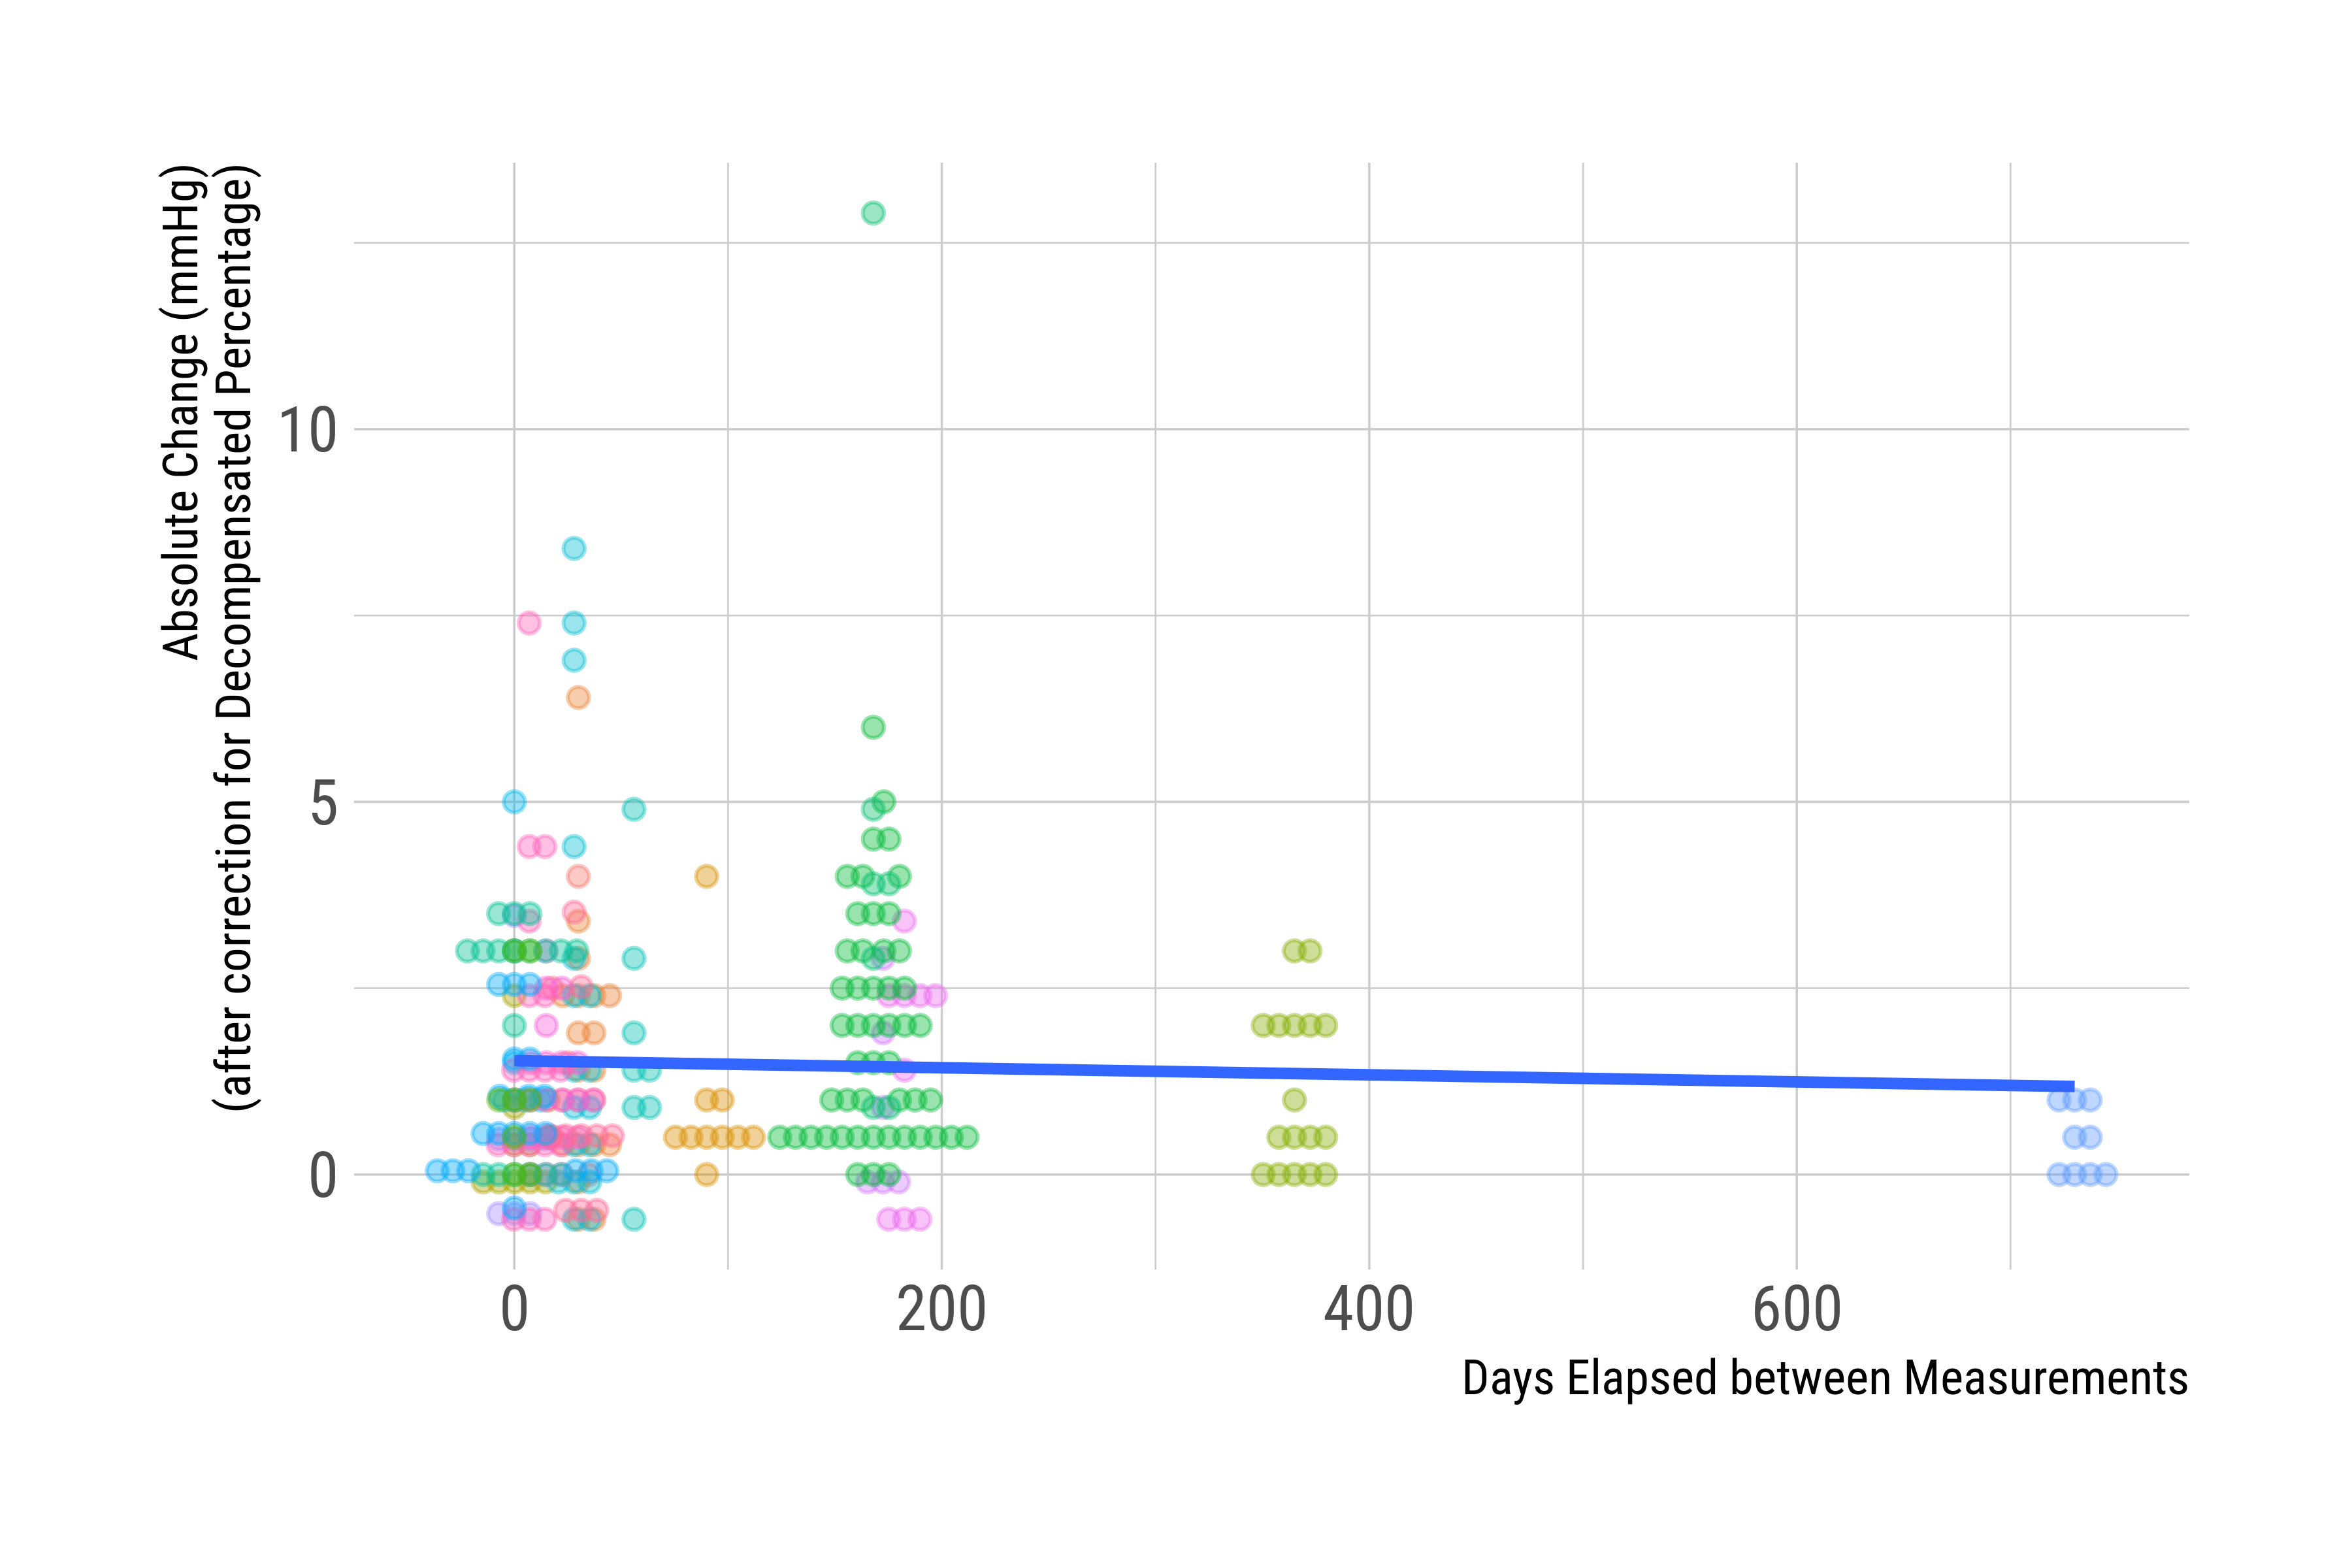
\includegraphics{figures/unnamed-chunk-32-1.png}

\begin{Shaded}
\begin{Highlighting}[]
\NormalTok{abs\_change\_distr }\OtherTok{\textless{}{-}}\NormalTok{ trt\_wide }\SpecialCharTok{\%\textgreater{}\%} 
  \FunctionTok{mutate}\NormalTok{(}\AttributeTok{decomp =} \FunctionTok{as.factor}\NormalTok{(decomp)) }\SpecialCharTok{\%\textgreater{}\%} 
  \FunctionTok{ggplot}\NormalTok{(}\FunctionTok{aes}\NormalTok{(}\AttributeTok{x=}\NormalTok{abschange, }\AttributeTok{colour=}\NormalTok{decomp, }\AttributeTok{fill=}\NormalTok{decomp, }\AttributeTok{group=}\NormalTok{decomp)) }\SpecialCharTok{+}
  \FunctionTok{geom\_density}\NormalTok{(}\FunctionTok{aes}\NormalTok{(}\AttributeTok{colour=}\NormalTok{decomp, }\AttributeTok{fill=}\NormalTok{decomp),}\AttributeTok{alpha=}\FloatTok{0.5}\NormalTok{) }\SpecialCharTok{+}
  \FunctionTok{theme}\NormalTok{(}\AttributeTok{legend.position=}\FunctionTok{c}\NormalTok{(}\FloatTok{0.5}\NormalTok{, }\FloatTok{0.9}\NormalTok{)) }\SpecialCharTok{+}
  \FunctionTok{scale\_color\_brewer}\NormalTok{(}\StringTok{"Patients"}\NormalTok{, }\AttributeTok{type =} \StringTok{"qual"}\NormalTok{, }\AttributeTok{palette =} \DecValTok{1}\NormalTok{) }\SpecialCharTok{+}
  \FunctionTok{scale\_fill\_brewer}\NormalTok{(}\StringTok{"Patients"}\NormalTok{, }\AttributeTok{type =} \StringTok{"qual"}\NormalTok{, }\AttributeTok{palette =} \DecValTok{1}\NormalTok{) }\SpecialCharTok{+}
  \FunctionTok{guides}\NormalTok{(}\AttributeTok{fill=}\ConstantTok{FALSE}\NormalTok{) }\SpecialCharTok{+}
  \FunctionTok{labs}\NormalTok{(}\AttributeTok{y =} \StringTok{""}\NormalTok{,}
       \AttributeTok{x =} \StringTok{"Absolute Change from first to second measurement (mmHg)"}\NormalTok{) }\SpecialCharTok{+}
  \FunctionTok{theme}\NormalTok{(}\AttributeTok{axis.text.y =} \FunctionTok{element\_blank}\NormalTok{(),}
        \AttributeTok{axis.ticks.y=}\FunctionTok{element\_blank}\NormalTok{())}

\NormalTok{abs\_change\_distr}
\end{Highlighting}
\end{Shaded}

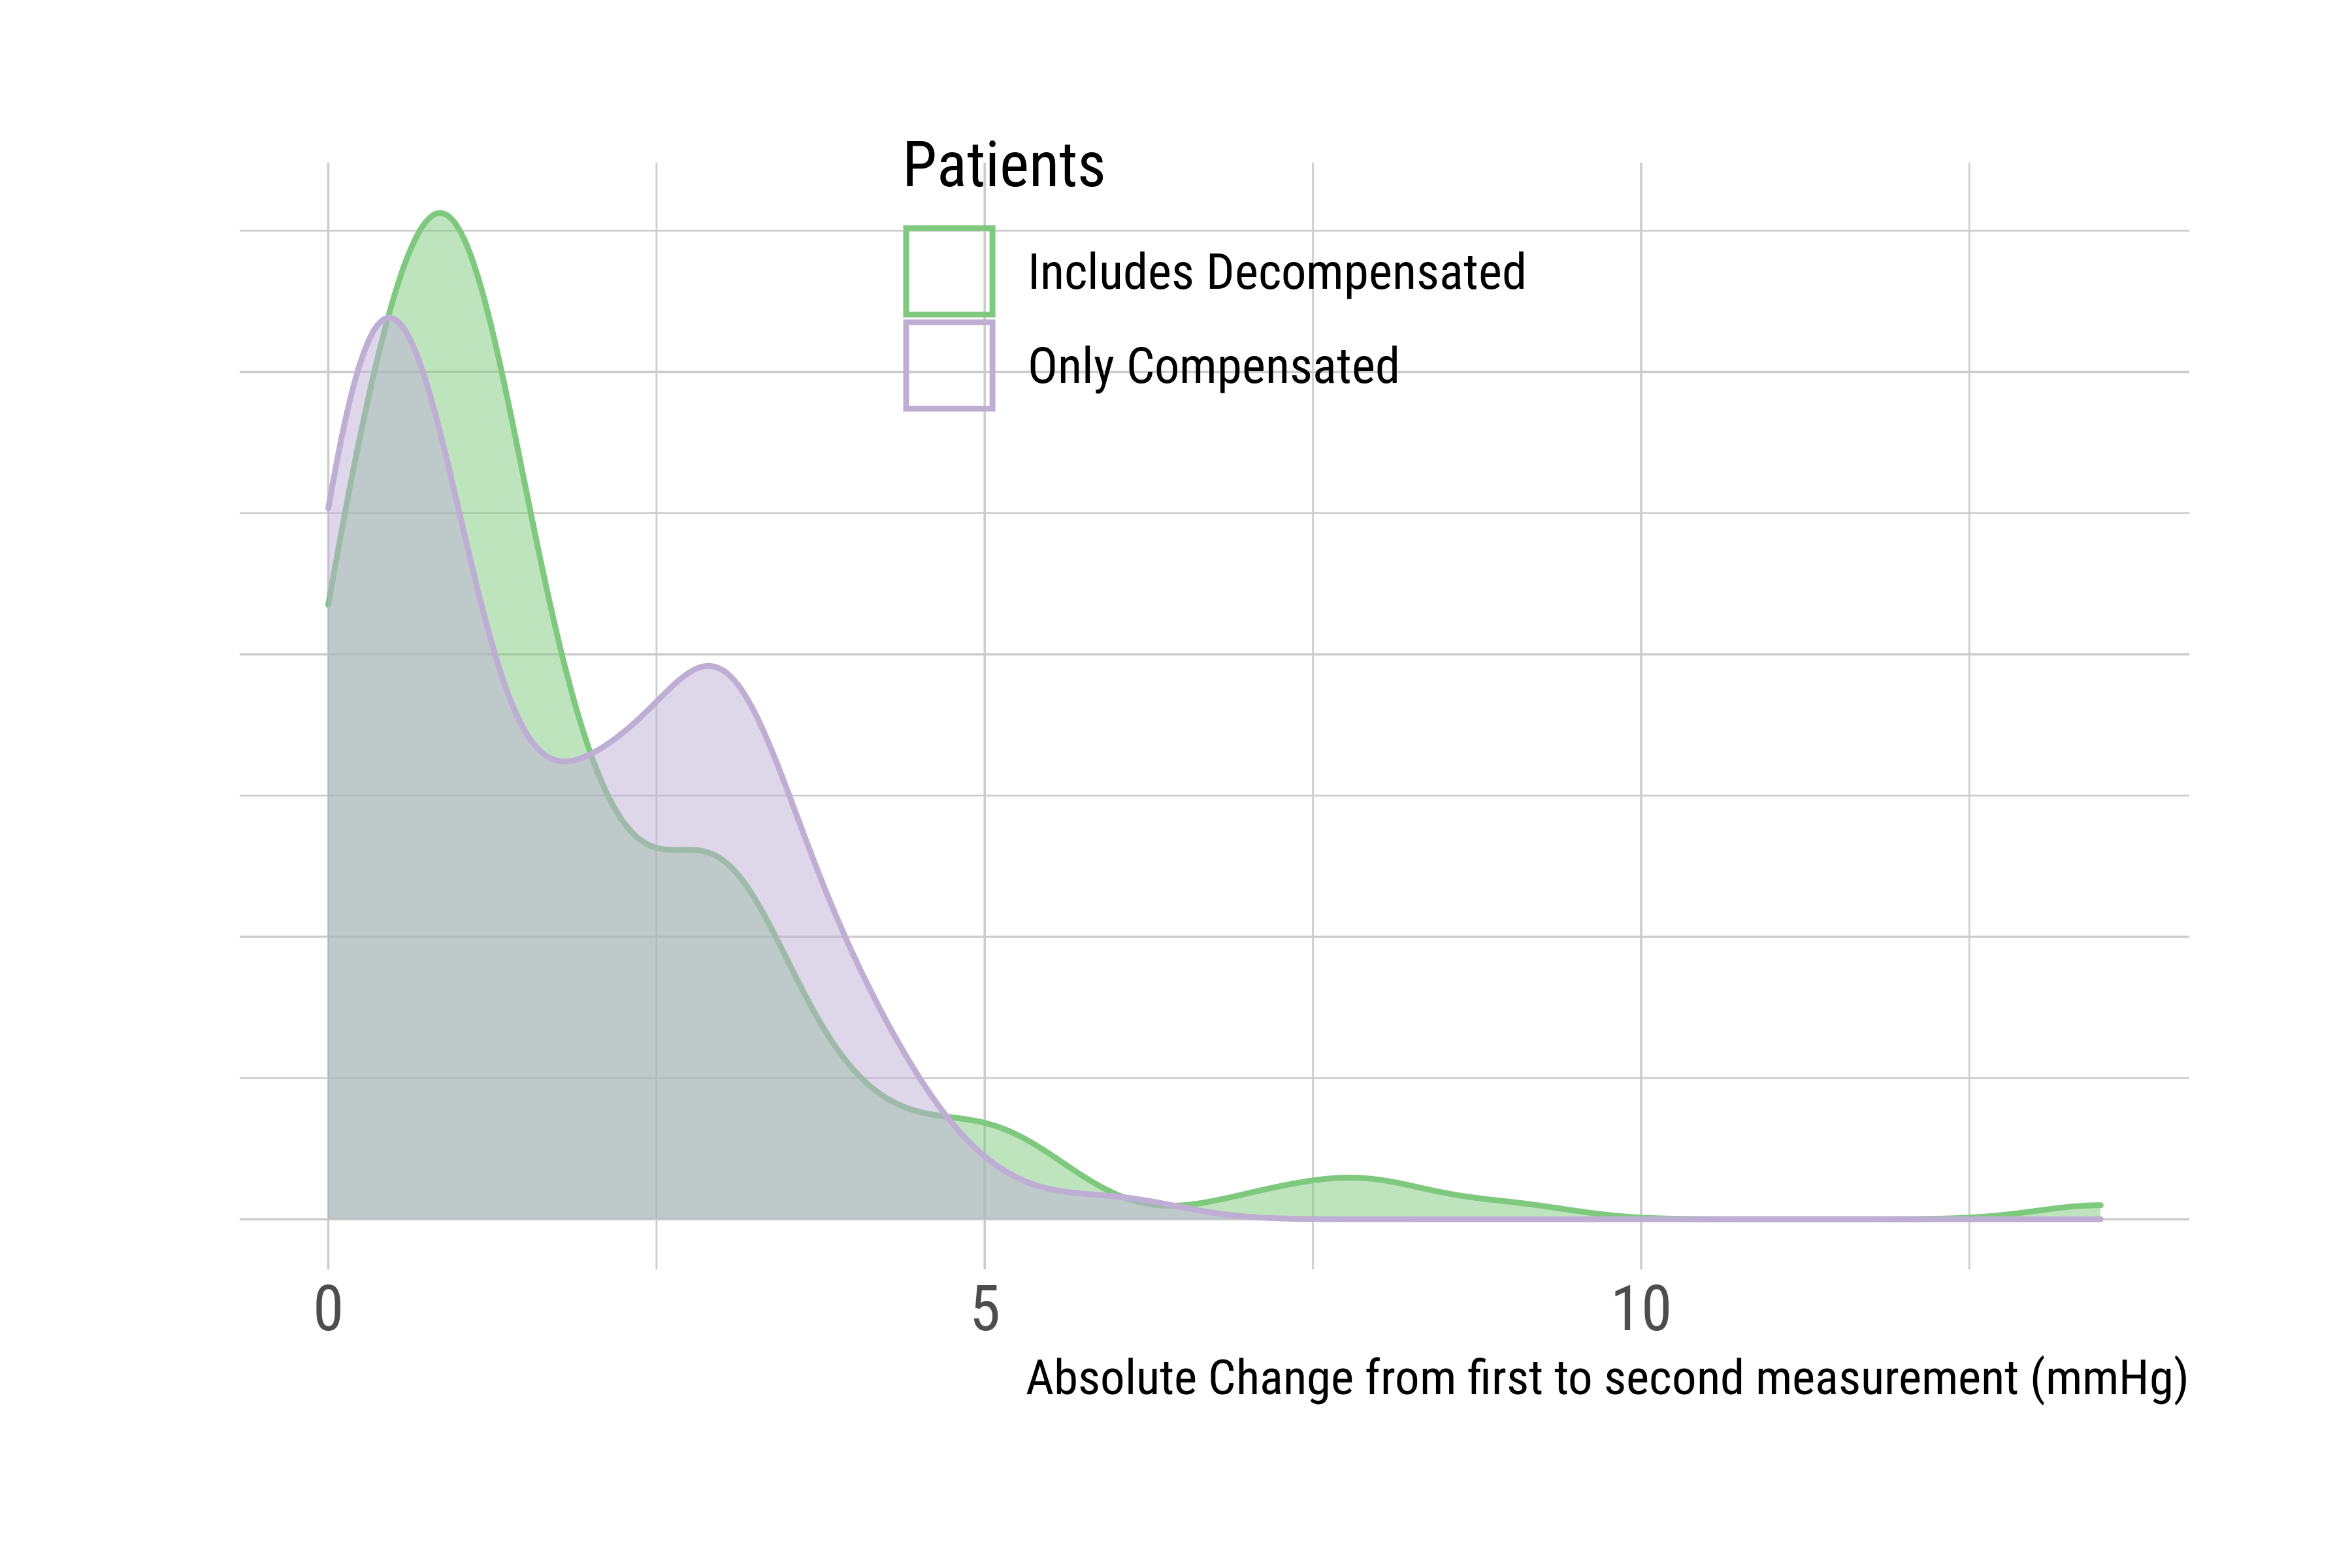
\includegraphics{figures/unnamed-chunk-32-2.png}

\hypertarget{percentage-decomp}{%
\subsection{Percentage Decomp}\label{percentage-decomp}}

\begin{Shaded}
\begin{Highlighting}[]
\FunctionTok{permTREND}\NormalTok{(}\AttributeTok{formula=}\NormalTok{abschange }\SpecialCharTok{\textasciitilde{}}\NormalTok{ Perc\_Decomp, }\AttributeTok{data=}\NormalTok{trt\_wide,}
          \AttributeTok{method=}\StringTok{"exact.mc"}\NormalTok{)}
\end{Highlighting}
\end{Shaded}

\begin{verbatim}
## 
##  Exact Permutation Test Estimated by Monte Carlo
## 
## data:  x and y
## p-value = 0.032
## alternative hypothesis: true correlation of x and y is not equal to 0
## sample estimates:
## correlation of x and y 
##              0.1262568 
## 
## p-value estimated from 999 Monte Carlo replications
## 99 percent confidence interval on p-value:
##  0.01384991 0.05601331
\end{verbatim}

\begin{Shaded}
\begin{Highlighting}[]
\NormalTok{permuco}\SpecialCharTok{::}\FunctionTok{lmperm}\NormalTok{(abschange }\SpecialCharTok{\textasciitilde{}}\NormalTok{ Perc\_Decomp, }\AttributeTok{data=}\NormalTok{trt\_wide)}
\end{Highlighting}
\end{Shaded}

\begin{verbatim}
## Table of marginal t-test of the betas
## Permutation test using freedman_lane to handle nuisance variables and 5000 permutations.
##             Estimate Std. Error t value parametric Pr(>|t|) permutation Pr(<t)
## (Intercept) 1.499246   0.153912   9.741           1.725e-19                   
## Perc_Decomp 0.005031   0.002367   2.126           3.439e-02             0.9812
##             permutation Pr(>t) permutation Pr(>|t|)
## (Intercept)                                        
## Perc_Decomp              0.019               0.0362
\end{verbatim}

\begin{Shaded}
\begin{Highlighting}[]
\NormalTok{decomp\_plot }\OtherTok{\textless{}{-}} \FunctionTok{ggplot}\NormalTok{(trt\_wide, }\FunctionTok{aes}\NormalTok{(}\AttributeTok{x=}\NormalTok{Perc\_Decomp, }\AttributeTok{y=}\NormalTok{abschange)) }\SpecialCharTok{+}
  \FunctionTok{geom\_beeswarm}\NormalTok{(}\FunctionTok{aes}\NormalTok{(}\AttributeTok{colour=}\FunctionTok{as.factor}\NormalTok{(Study), }
                    \AttributeTok{group=}\FunctionTok{as.factor}\NormalTok{(Perc\_Decomp)),}
                \AttributeTok{alpha=}\FloatTok{0.4}\NormalTok{, }\AttributeTok{cex=}\DecValTok{1}\NormalTok{) }\SpecialCharTok{+}
  \FunctionTok{guides}\NormalTok{(}\AttributeTok{colour=}\ConstantTok{FALSE}\NormalTok{) }\SpecialCharTok{+} 
  \FunctionTok{geom\_smooth}\NormalTok{(}\AttributeTok{method=}\StringTok{"lm"}\NormalTok{, }\AttributeTok{se =} \ConstantTok{FALSE}\NormalTok{) }\SpecialCharTok{+}
  \FunctionTok{labs}\NormalTok{(}\AttributeTok{x=}\StringTok{"Decompensated Patients (\%)"}\NormalTok{,}
       \AttributeTok{y=}\StringTok{"Absolute Change (mmHg)"}\NormalTok{)}

\NormalTok{decomp\_plot}
\end{Highlighting}
\end{Shaded}

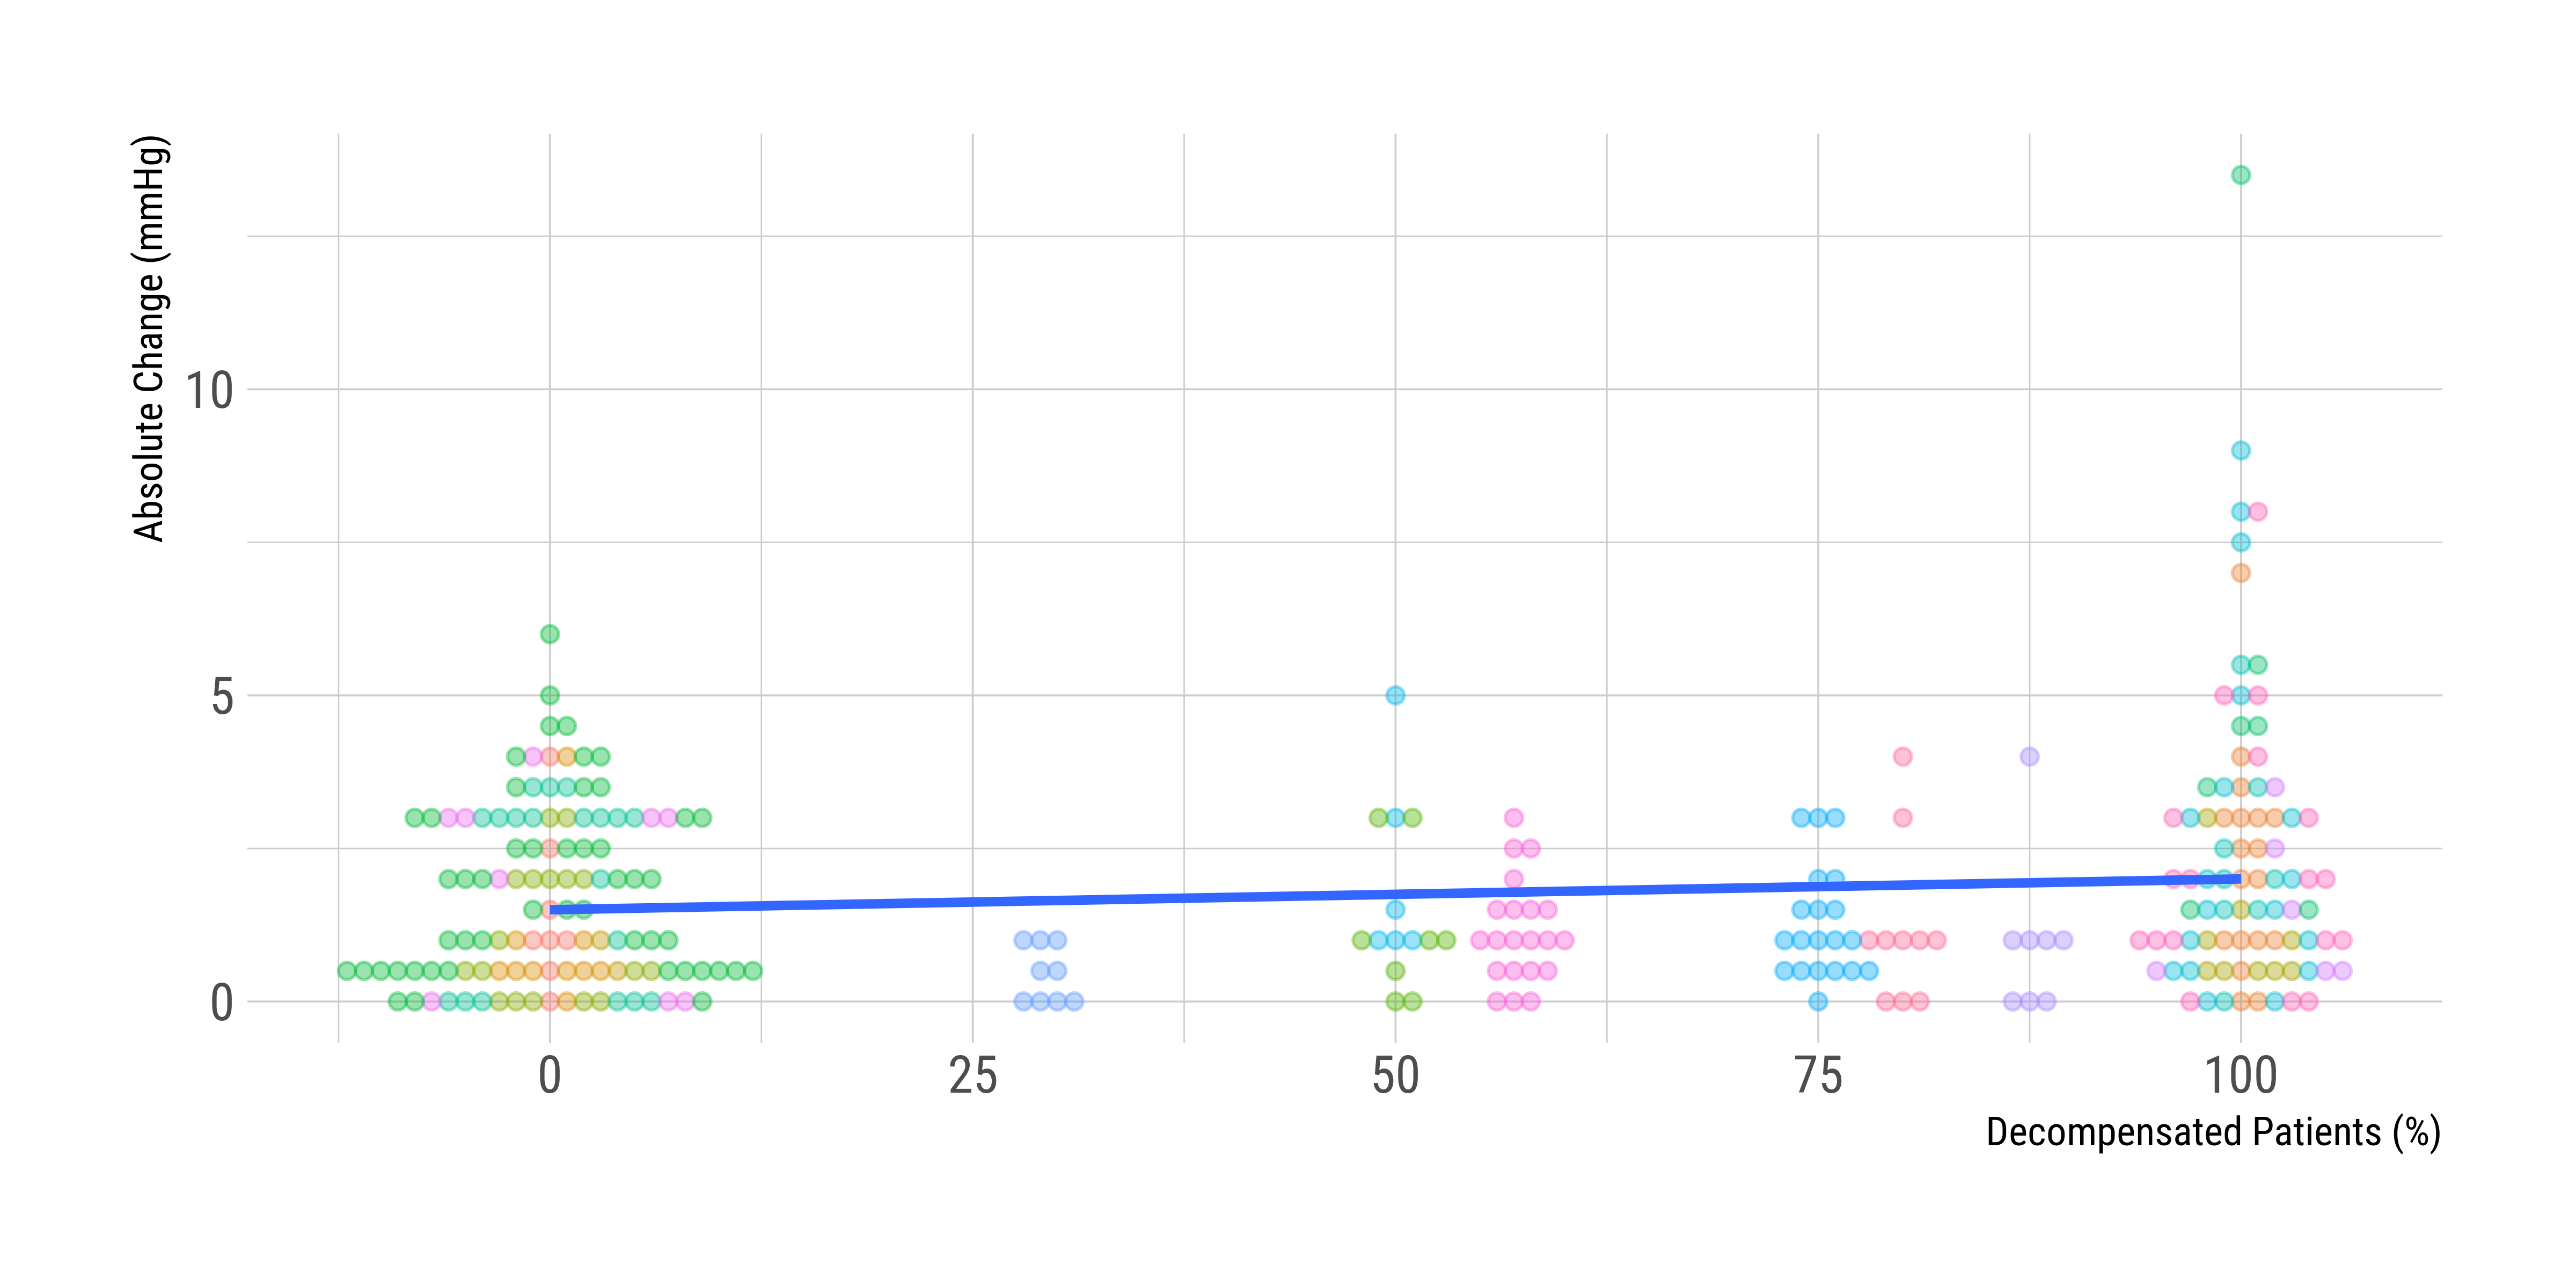
\includegraphics{figures/unnamed-chunk-34-1.png}

\hypertarget{days-elapsed}{%
\subsection{Days elapsed}\label{days-elapsed}}

\begin{Shaded}
\begin{Highlighting}[]
\NormalTok{permuco}\SpecialCharTok{::}\FunctionTok{lmperm}\NormalTok{(abschange }\SpecialCharTok{\textasciitilde{}}\NormalTok{ Days }\SpecialCharTok{+}\NormalTok{ Perc\_Decomp, }\AttributeTok{data=}\NormalTok{trt\_wide)}
\end{Highlighting}
\end{Shaded}

\begin{verbatim}
## Table of marginal t-test of the betas
## Permutation test using freedman_lane to handle nuisance variables and 5000 permutations.
##               Estimate Std. Error t value parametric Pr(>|t|)
## (Intercept)  1.6031874  0.1994382  8.0385           2.624e-14
## Days        -0.0006133  0.0007477 -0.8202           4.128e-01
## Perc_Decomp  0.0041622  0.0025941  1.6045           1.097e-01
##             permutation Pr(<t) permutation Pr(>t) permutation Pr(>|t|)
## (Intercept)                                                           
## Days                    0.2076             0.7926               0.3990
## Perc_Decomp             0.9524             0.0478               0.1026
\end{verbatim}

Now let's plot, after correcting for the effect of the patient groups.

\begin{Shaded}
\begin{Highlighting}[]
\NormalTok{correct\_for\_decomp }\OtherTok{\textless{}{-}} \ControlFlowTok{function}\NormalTok{(formula) \{}
  
\NormalTok{  formula }\OtherTok{\textless{}{-}} \FunctionTok{as.formula}\NormalTok{(formula)}
  
\NormalTok{  coefficients }\OtherTok{\textless{}{-}} \FunctionTok{coef}\NormalTok{(permuco}\SpecialCharTok{::}\FunctionTok{lmperm}\NormalTok{(formula, }
                                       \AttributeTok{data=}\NormalTok{trt\_wide))}

\NormalTok{  predicted }\OtherTok{\textless{}{-}} \FunctionTok{as.character}\NormalTok{(formula[}\DecValTok{2}\NormalTok{])}
  
\NormalTok{  after\_decomp\_corr }\OtherTok{\textless{}{-}}\NormalTok{ trt\_wide[[predicted]] }\SpecialCharTok{{-}} 
\NormalTok{    trt\_wide[[}\StringTok{"Perc\_Decomp"}\NormalTok{]] }\SpecialCharTok{*}\NormalTok{ coefficients[}\FunctionTok{which}\NormalTok{(}\FunctionTok{names}\NormalTok{(coefficients)}\SpecialCharTok{==}\StringTok{"Perc\_Decomp"}\NormalTok{)]}
  
  \FunctionTok{return}\NormalTok{(after\_decomp\_corr)}
  
\NormalTok{\}}

\NormalTok{days\_plot }\OtherTok{\textless{}{-}}\NormalTok{ trt\_wide }\SpecialCharTok{\%\textgreater{}\%} 
  \FunctionTok{mutate}\NormalTok{(}\AttributeTok{abschange\_dccorr =} \FunctionTok{correct\_for\_decomp}\NormalTok{(abschange }\SpecialCharTok{\textasciitilde{}}\NormalTok{ Days }\SpecialCharTok{+}\NormalTok{ Perc\_Decomp)) }\SpecialCharTok{\%\textgreater{}\%} 
  \FunctionTok{ggplot}\NormalTok{(}\FunctionTok{aes}\NormalTok{(}\AttributeTok{x=}\NormalTok{Days, }\AttributeTok{y=}\NormalTok{abschange\_dccorr)) }\SpecialCharTok{+}
  \FunctionTok{geom\_beeswarm}\NormalTok{(}\FunctionTok{aes}\NormalTok{(}\AttributeTok{colour=}\NormalTok{Study, }\AttributeTok{group=}\NormalTok{Study), }\AttributeTok{alpha=}\FloatTok{0.4}\NormalTok{, }\AttributeTok{cex=}\DecValTok{1}\NormalTok{) }\SpecialCharTok{+}
  \FunctionTok{guides}\NormalTok{(}\AttributeTok{colour=}\ConstantTok{FALSE}\NormalTok{) }\SpecialCharTok{+} 
  \FunctionTok{geom\_smooth}\NormalTok{(}\AttributeTok{method=}\StringTok{"lm"}\NormalTok{, }\AttributeTok{se=}\ConstantTok{FALSE}\NormalTok{) }\SpecialCharTok{+}
  \FunctionTok{labs}\NormalTok{(}\AttributeTok{y=}\StringTok{"Absolute Change (mmHg)}\SpecialCharTok{\textbackslash{}n}\StringTok{(after correction for Decompensated Percentage)"}\NormalTok{,}
       \AttributeTok{x=}\StringTok{"Days Elapsed between Measurements"}\NormalTok{)}

\NormalTok{days\_plot}
\end{Highlighting}
\end{Shaded}

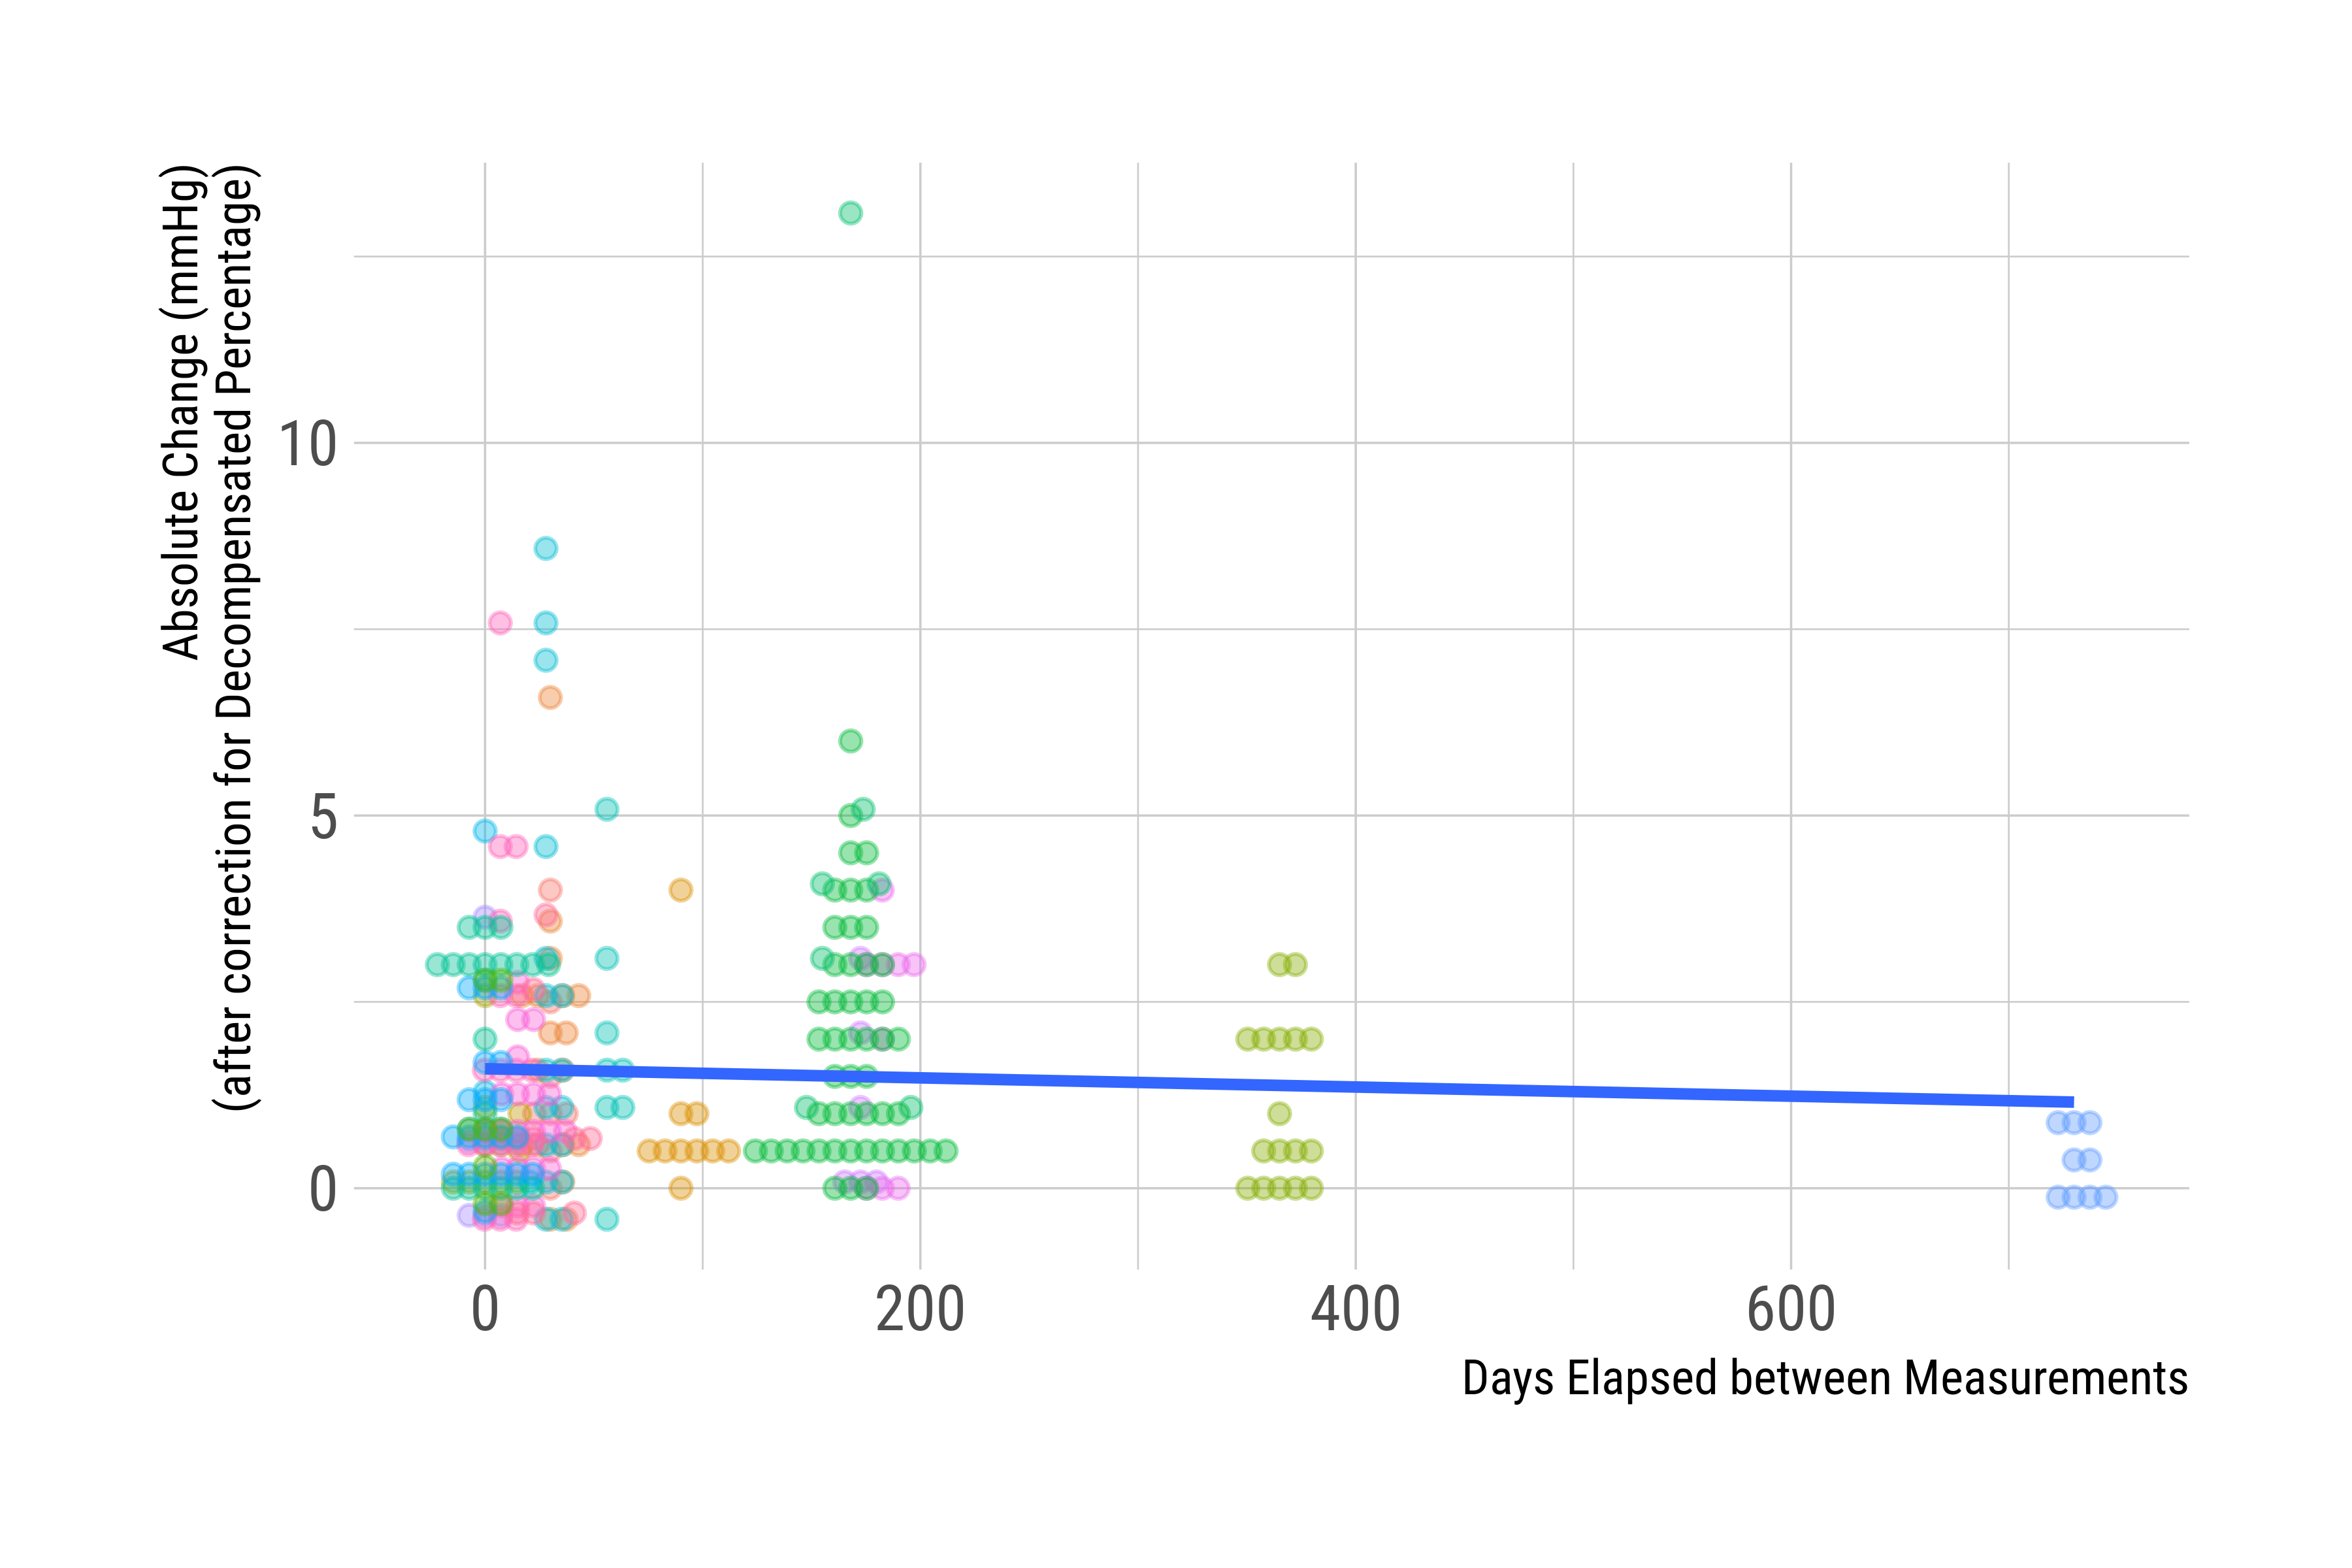
\includegraphics{figures/unnamed-chunk-36-1.png}

\hypertarget{percentage-alcoholic}{%
\subsection{Percentage Alcoholic}\label{percentage-alcoholic}}

\begin{Shaded}
\begin{Highlighting}[]
\NormalTok{permuco}\SpecialCharTok{::}\FunctionTok{lmperm}\NormalTok{(abschange }\SpecialCharTok{\textasciitilde{}}\NormalTok{ Perc\_Alc }\SpecialCharTok{+}\NormalTok{ Perc\_Decomp, }\AttributeTok{data=}\NormalTok{trt\_wide)}
\end{Highlighting}
\end{Shaded}

\begin{verbatim}
## Table of marginal t-test of the betas
## Permutation test using freedman_lane to handle nuisance variables and 5000 permutations.
##             Estimate Std. Error t value parametric Pr(>|t|) permutation Pr(<t)
## (Intercept)  1.94758   0.166155  11.721           4.711e-26                   
## Perc_Alc    -0.02579   0.004560  -5.655           3.869e-08              2e-04
## Perc_Decomp  0.01881   0.003313   5.677           3.447e-08              1e+00
##             permutation Pr(>t) permutation Pr(>|t|)
## (Intercept)                                        
## Perc_Alc                 1e+00                2e-04
## Perc_Decomp              2e-04                2e-04
\end{verbatim}

\begin{Shaded}
\begin{Highlighting}[]
\FunctionTok{permTREND}\NormalTok{(}\AttributeTok{formula=}\NormalTok{abschange }\SpecialCharTok{\textasciitilde{}}\NormalTok{ Perc\_Alc, }\AttributeTok{data=}\NormalTok{trt\_wide\_c,}
          \AttributeTok{method=}\StringTok{"exact.mc"}\NormalTok{)}
\end{Highlighting}
\end{Shaded}

\begin{verbatim}
## 
##  Exact Permutation Test Estimated by Monte Carlo
## 
## data:  x and y
## p-value = 0.01
## alternative hypothesis: true correlation of x and y is not equal to 0
## sample estimates:
## correlation of x and y 
##             -0.2373197 
## 
## p-value estimated from 999 Monte Carlo replications
## 99 percent confidence interval on p-value:
##  0.001347329 0.025105152
\end{verbatim}

\begin{Shaded}
\begin{Highlighting}[]
\FunctionTok{permTREND}\NormalTok{(}\AttributeTok{formula=}\NormalTok{abschange }\SpecialCharTok{\textasciitilde{}}\NormalTok{ Perc\_Alc, }\AttributeTok{data=}\NormalTok{trt\_wide\_dc,}
          \AttributeTok{method=}\StringTok{"exact.mc"}\NormalTok{)}
\end{Highlighting}
\end{Shaded}

\begin{verbatim}
## 
##  Exact Permutation Test Estimated by Monte Carlo
## 
## data:  x and y
## p-value = 0.006
## alternative hypothesis: true correlation of x and y is not equal to 0
## sample estimates:
## correlation of x and y 
##             -0.2099865 
## 
## p-value estimated from 999 Monte Carlo replications
## 99 percent confidence interval on p-value:
##  0.0002072893 0.0184986927
\end{verbatim}

\begin{Shaded}
\begin{Highlighting}[]
\NormalTok{perc\_alc\_plot }\OtherTok{\textless{}{-}}\NormalTok{ trt\_wide }\SpecialCharTok{\%\textgreater{}\%} 
  \FunctionTok{mutate}\NormalTok{(}\AttributeTok{abschange\_dccorr =} \FunctionTok{correct\_for\_decomp}\NormalTok{(abschange }\SpecialCharTok{\textasciitilde{}}\NormalTok{ Perc\_Alc }\SpecialCharTok{+}\NormalTok{ Perc\_Decomp)) }\SpecialCharTok{\%\textgreater{}\%} 
  \FunctionTok{ggplot}\NormalTok{(}\FunctionTok{aes}\NormalTok{(}\AttributeTok{x=}\NormalTok{Perc\_Alc, }\AttributeTok{y=}\NormalTok{abschange\_dccorr)) }\SpecialCharTok{+}
  \FunctionTok{geom\_beeswarm}\NormalTok{(}\FunctionTok{aes}\NormalTok{(}\AttributeTok{colour=}\NormalTok{Study, }\AttributeTok{group=}\NormalTok{Study), }\AttributeTok{alpha=}\FloatTok{0.4}\NormalTok{, }\AttributeTok{cex=}\DecValTok{1}\NormalTok{) }\SpecialCharTok{+}
  \FunctionTok{guides}\NormalTok{(}\AttributeTok{colour=}\ConstantTok{FALSE}\NormalTok{) }\SpecialCharTok{+} 
  \FunctionTok{geom\_smooth}\NormalTok{(}\AttributeTok{method=}\StringTok{"lm"}\NormalTok{, }\AttributeTok{se=}\ConstantTok{FALSE}\NormalTok{) }\SpecialCharTok{+}
  \FunctionTok{labs}\NormalTok{(}\AttributeTok{y=}\StringTok{"Absolute Change (mmHg)}\SpecialCharTok{\textbackslash{}n}\StringTok{(after correction for Decompensated Percentage)"}\NormalTok{,}
       \AttributeTok{x=}\StringTok{"Percentage of Alcoholic Patients (\%)"}\NormalTok{)}

\NormalTok{perc\_alc\_plot}
\end{Highlighting}
\end{Shaded}

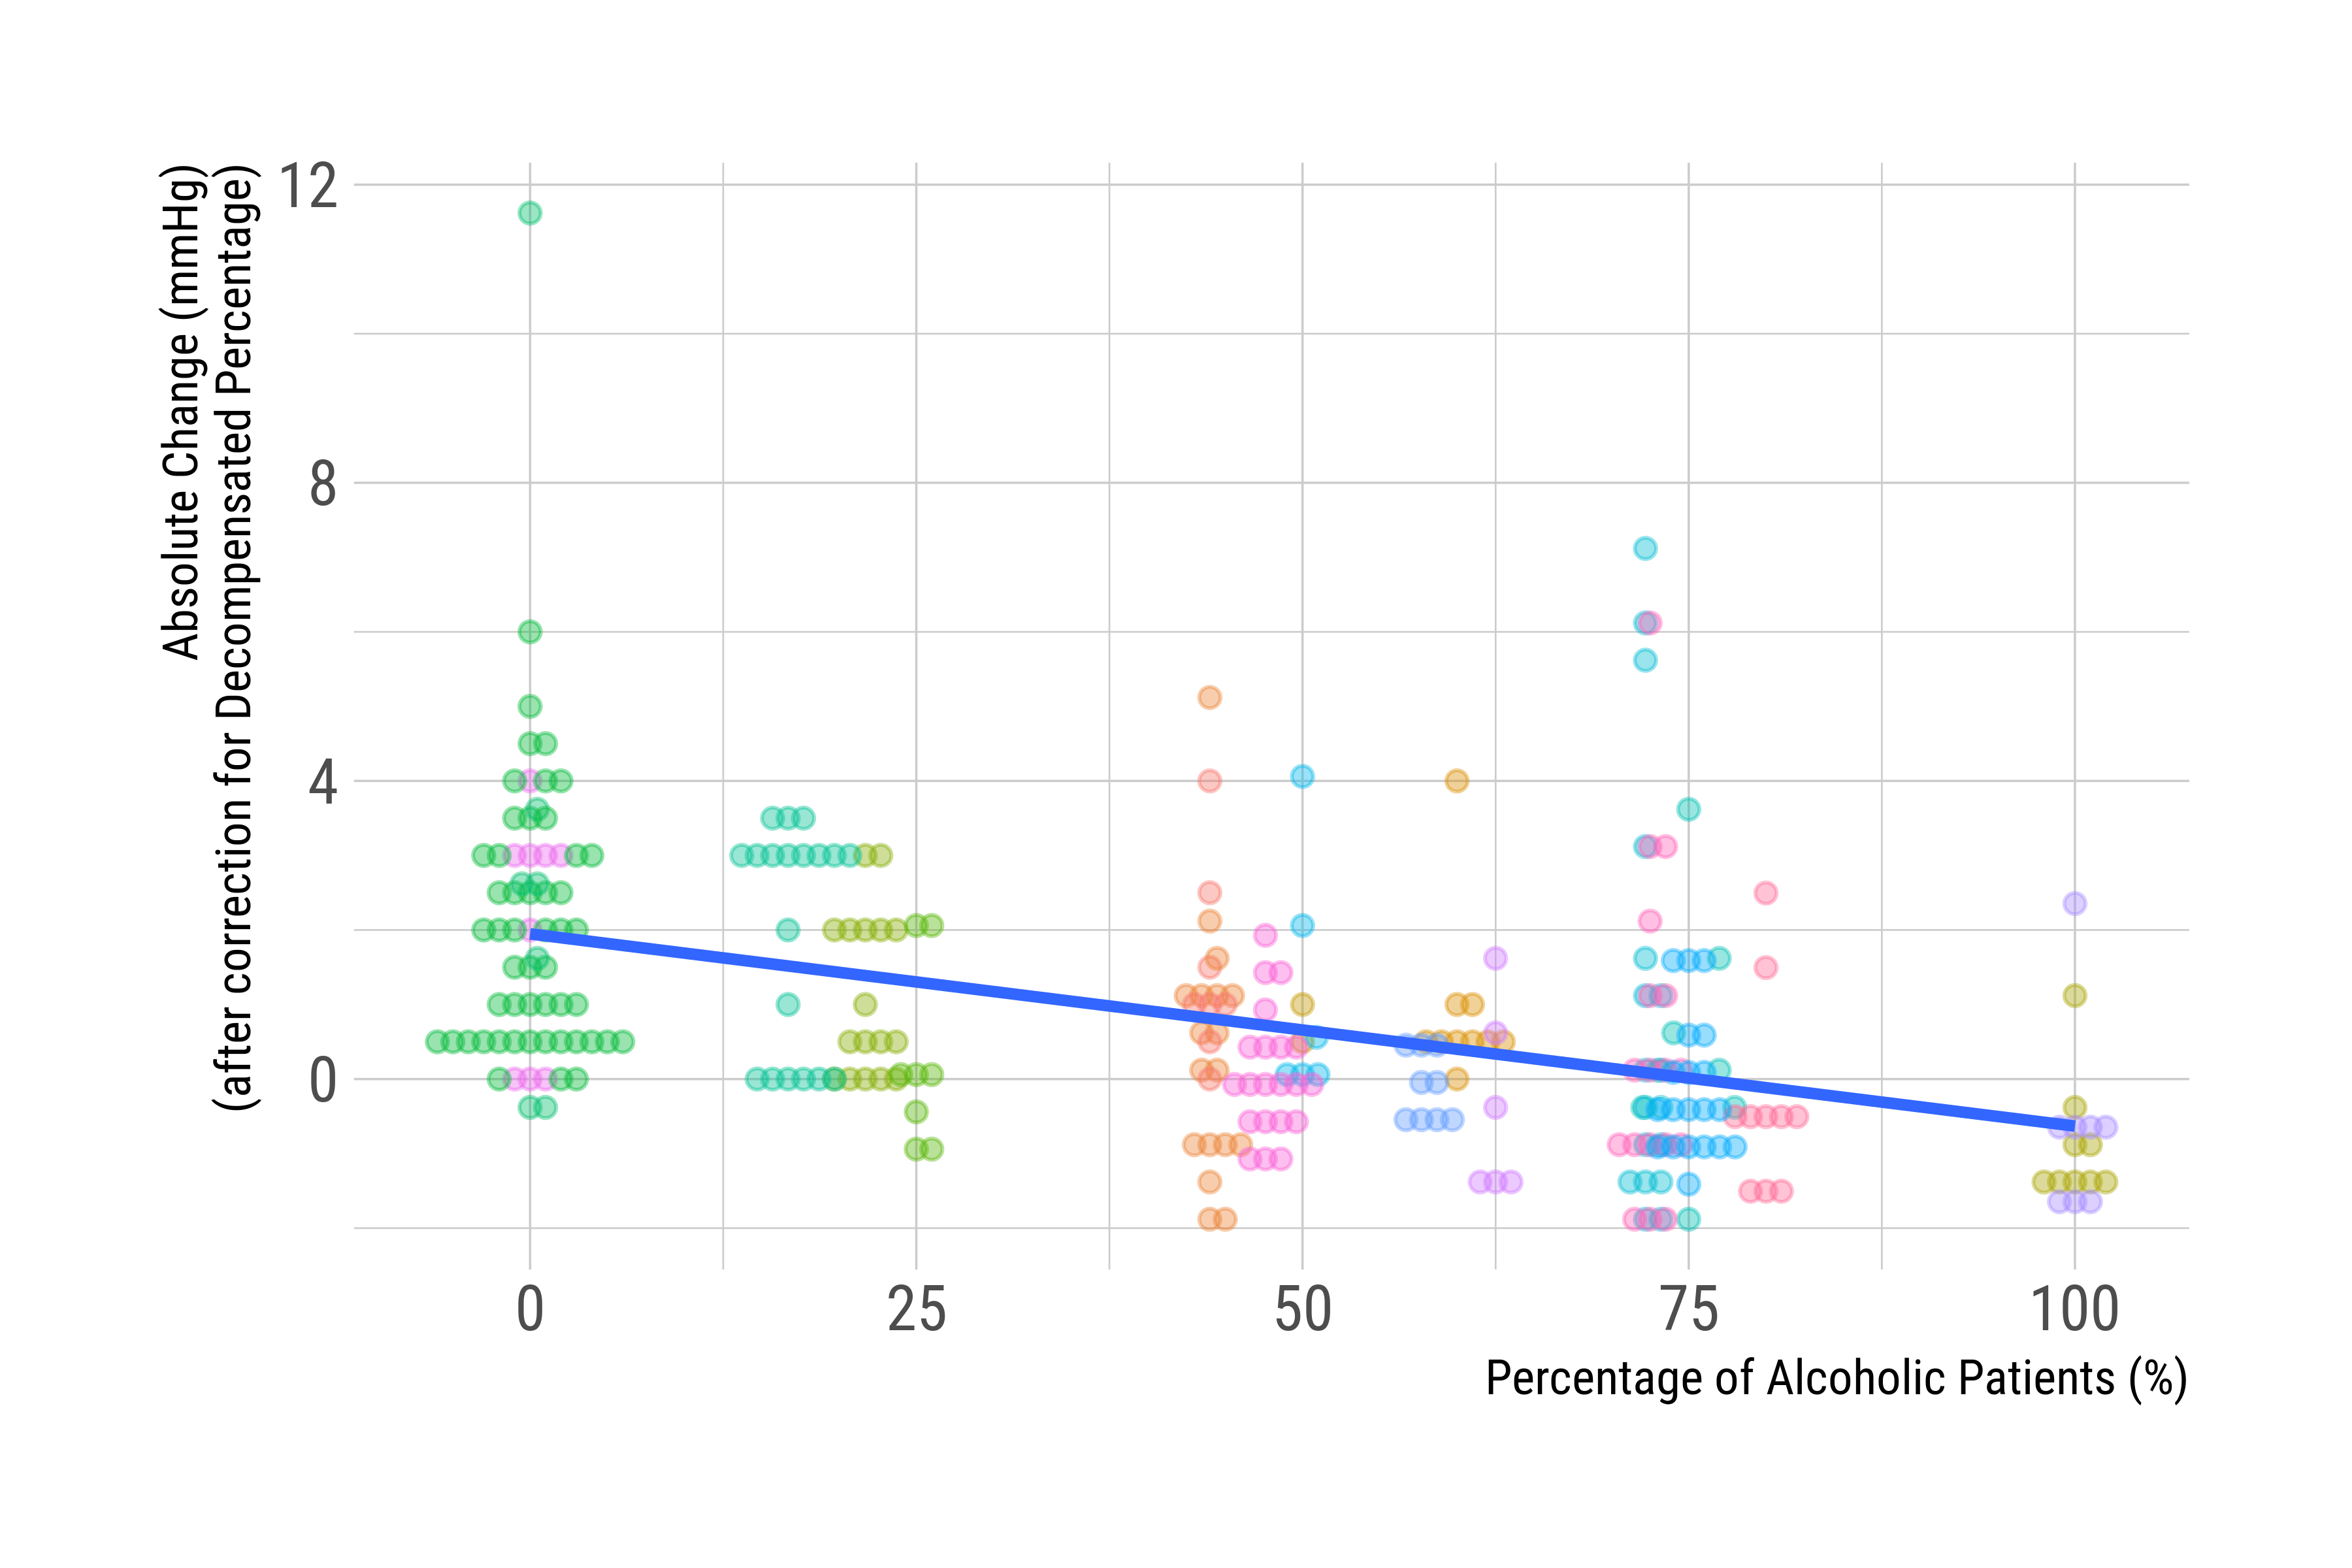
\includegraphics{figures/unnamed-chunk-38-1.png}

\hypertarget{multicentre}{%
\subsection{Multicentre}\label{multicentre}}

\begin{Shaded}
\begin{Highlighting}[]
\NormalTok{permuco}\SpecialCharTok{::}\FunctionTok{lmperm}\NormalTok{(abschange }\SpecialCharTok{\textasciitilde{}}\NormalTok{ Centre }\SpecialCharTok{+}\NormalTok{ Perc\_Decomp, }\AttributeTok{data=}\NormalTok{trt\_wide)}
\end{Highlighting}
\end{Shaded}

\begin{verbatim}
## Table of marginal t-test of the betas
## Permutation test using freedman_lane to handle nuisance variables and 5000 permutations.
##                      Estimate Std. Error t value parametric Pr(>|t|)
## (Intercept)          1.663139   0.165791  10.032           2.056e-20
## CentreSingle-centre -0.544349   0.216320  -2.516           1.242e-02
## Perc_Decomp          0.007055   0.002478   2.846           4.750e-03
##                     permutation Pr(<t) permutation Pr(>t) permutation Pr(>|t|)
## (Intercept)                                                                   
## CentreSingle-centre             0.0062              0.994               0.0136
## Perc_Decomp                     0.9982              0.002               0.0040
\end{verbatim}

\begin{Shaded}
\begin{Highlighting}[]
\NormalTok{centre\_plot }\OtherTok{\textless{}{-}}\NormalTok{ trt\_wide }\SpecialCharTok{\%\textgreater{}\%} 
  \FunctionTok{mutate}\NormalTok{(}\AttributeTok{abschange\_dccorr =} \FunctionTok{correct\_for\_decomp}\NormalTok{(abschange }\SpecialCharTok{\textasciitilde{}}\NormalTok{ Centre }\SpecialCharTok{+}\NormalTok{ Perc\_Decomp)) }\SpecialCharTok{\%\textgreater{}\%} 
  \FunctionTok{ggplot}\NormalTok{(}\FunctionTok{aes}\NormalTok{(}\AttributeTok{x=}\NormalTok{Centre, }\AttributeTok{y=}\NormalTok{abschange\_dccorr)) }\SpecialCharTok{+}
  \FunctionTok{geom\_beeswarm}\NormalTok{(}\FunctionTok{aes}\NormalTok{(}\AttributeTok{colour=}\NormalTok{Study, }\AttributeTok{group=}\NormalTok{Study), }\AttributeTok{alpha=}\FloatTok{0.4}\NormalTok{, }\AttributeTok{cex=}\DecValTok{1}\NormalTok{) }\SpecialCharTok{+}
  \FunctionTok{guides}\NormalTok{(}\AttributeTok{colour=}\ConstantTok{FALSE}\NormalTok{) }\SpecialCharTok{+} 
  \FunctionTok{geom\_smooth}\NormalTok{(}\AttributeTok{method=}\StringTok{"lm"}\NormalTok{, }\AttributeTok{se=}\ConstantTok{FALSE}\NormalTok{) }\SpecialCharTok{+}
  \FunctionTok{labs}\NormalTok{(}\AttributeTok{y=}\StringTok{"Absolute Change (mmHg)}\SpecialCharTok{\textbackslash{}n}\StringTok{(after correction for Decompensated Percentage)"}\NormalTok{)}

\NormalTok{centre\_plot}
\end{Highlighting}
\end{Shaded}

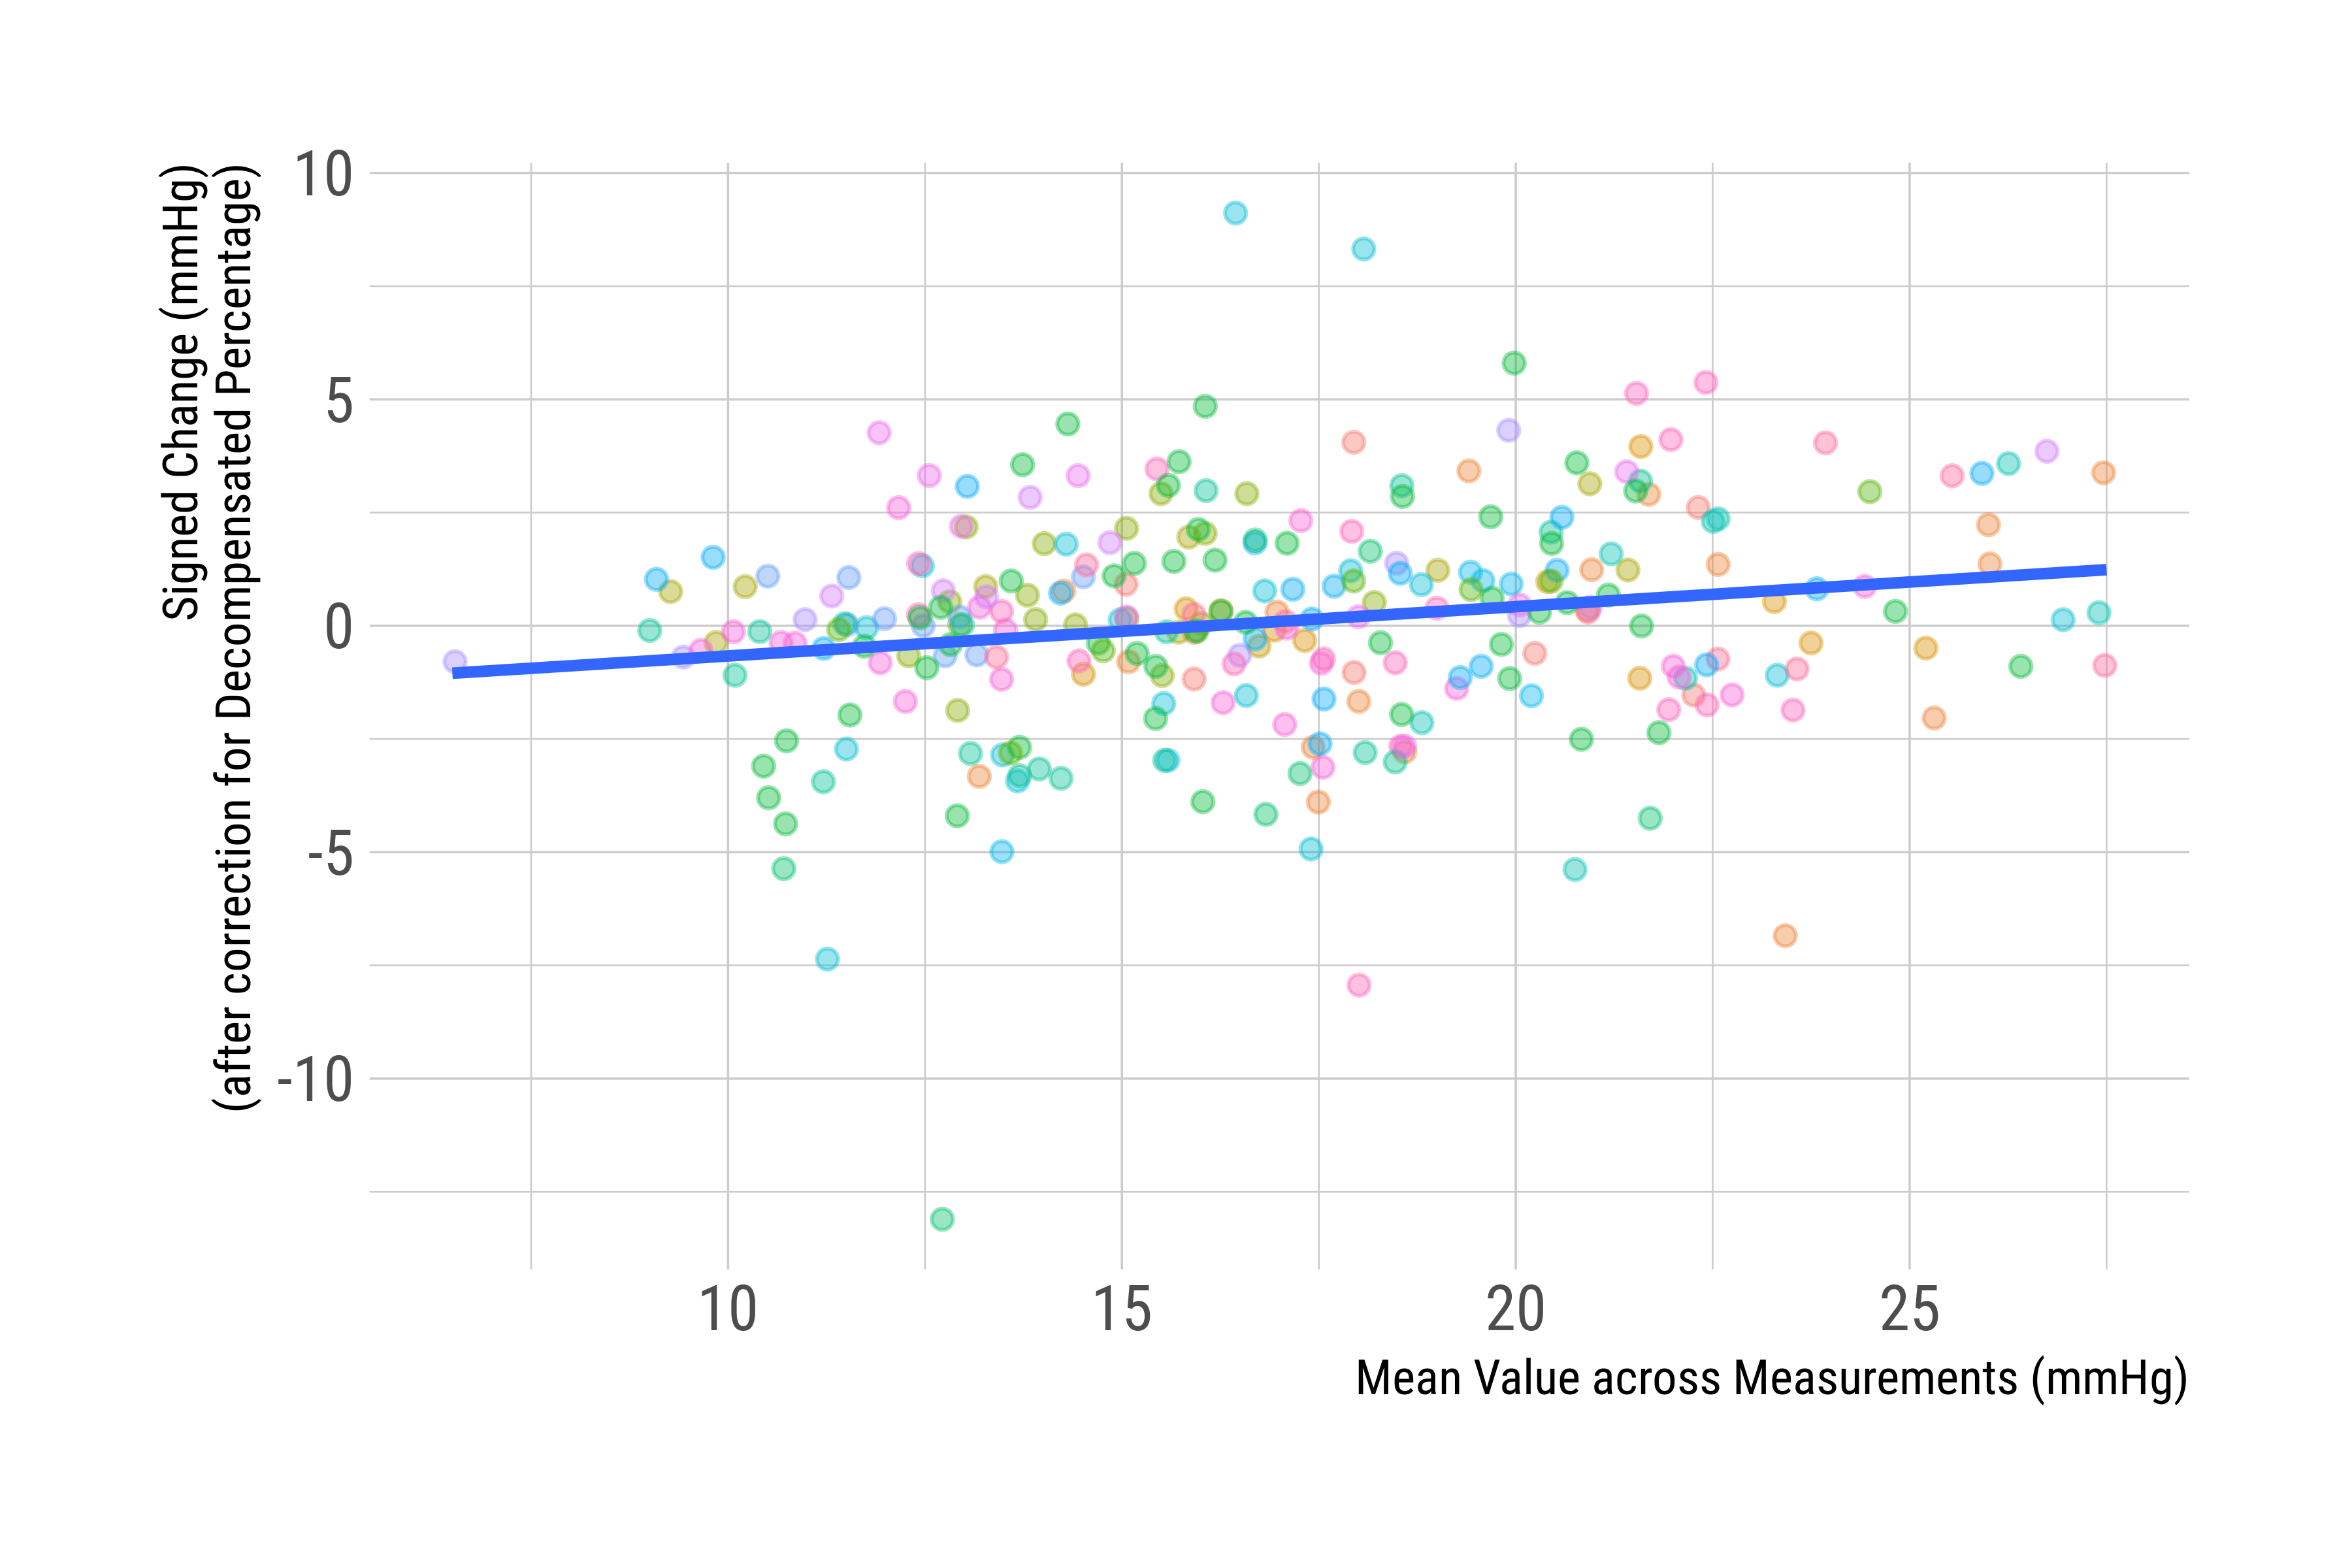
\includegraphics{figures/unnamed-chunk-40-1.png}

\hypertarget{combined-model}{%
\subsection{Combined Model}\label{combined-model}}

\begin{Shaded}
\begin{Highlighting}[]
\NormalTok{permuco}\SpecialCharTok{::}\FunctionTok{lmperm}\NormalTok{(abschange }\SpecialCharTok{\textasciitilde{}}\NormalTok{ Perc\_Decomp }\SpecialCharTok{+}\NormalTok{ Centre }\SpecialCharTok{+}\NormalTok{ Perc\_Alc, }\AttributeTok{data=}\NormalTok{trt\_wide)}
\end{Highlighting}
\end{Shaded}

\begin{verbatim}
## Table of marginal t-test of the betas
## Permutation test using freedman_lane to handle nuisance variables and 5000 permutations.
##                     Estimate Std. Error  t value parametric Pr(>|t|)
## (Intercept)          1.94534   0.168789 11.52527           2.287e-25
## Perc_Decomp          0.01884   0.003349  5.62673           4.493e-08
## CentreSingle-centre  0.01892   0.236163  0.08012           9.362e-01
## Perc_Alc            -0.02599   0.005198 -4.99906           1.023e-06
##                     permutation Pr(<t) permutation Pr(>t) permutation Pr(>|t|)
## (Intercept)                                                                   
## Perc_Decomp                     1.0000             0.0002               0.0002
## CentreSingle-centre             0.5338             0.4664               0.9270
## Perc_Alc                        0.0002             1.0000               0.0002
\end{verbatim}

\begin{Shaded}
\begin{Highlighting}[]
\NormalTok{permuco}\SpecialCharTok{::}\FunctionTok{lmperm}\NormalTok{(abschange }\SpecialCharTok{\textasciitilde{}}\NormalTok{ Centre }\SpecialCharTok{+}\NormalTok{ Perc\_Alc, }\AttributeTok{data=}\NormalTok{trt\_wide\_c)}
\end{Highlighting}
\end{Shaded}

\begin{verbatim}
## Table of marginal t-test of the betas
## Permutation test using freedman_lane to handle nuisance variables and 5000 permutations.
##                     Estimate Std. Error t value parametric Pr(>|t|)
## (Intercept)          1.99513   0.170383  11.710           3.636e-21
## CentreSingle-centre -0.38265   0.310236  -1.233           2.200e-01
## Perc_Alc            -0.01289   0.007501  -1.718           8.858e-02
##                     permutation Pr(<t) permutation Pr(>t) permutation Pr(>|t|)
## (Intercept)                                                                   
## CentreSingle-centre             0.1070             0.8932               0.2218
## Perc_Alc                        0.0474             0.9528               0.0924
\end{verbatim}

\begin{Shaded}
\begin{Highlighting}[]
\NormalTok{permuco}\SpecialCharTok{::}\FunctionTok{lmperm}\NormalTok{(abschange }\SpecialCharTok{\textasciitilde{}}\NormalTok{ Centre }\SpecialCharTok{+}\NormalTok{ Perc\_Alc, }\AttributeTok{data=}\NormalTok{trt\_wide\_dc)}
\end{Highlighting}
\end{Shaded}

\begin{verbatim}
## Table of marginal t-test of the betas
## Permutation test using freedman_lane to handle nuisance variables and 5000 permutations.
##                     Estimate Std. Error t value parametric Pr(>|t|)
## (Intercept)          2.99299   0.440666   6.792           1.967e-10
## CentreSingle-centre  0.37572   0.372646   1.008           3.148e-01
## Perc_Alc            -0.02274   0.008097  -2.808           5.587e-03
##                     permutation Pr(<t) permutation Pr(>t) permutation Pr(>|t|)
## (Intercept)                                                                   
## CentreSingle-centre             0.8450             0.1552               0.3112
## Perc_Alc                        0.0066             0.9936               0.0078
\end{verbatim}

Let's examine why this might be.

\begin{Shaded}
\begin{Highlighting}[]
\NormalTok{trt\_wide }\SpecialCharTok{\%\textgreater{}\%} 
  \FunctionTok{ggplot}\NormalTok{(}\FunctionTok{aes}\NormalTok{(}\AttributeTok{y=}\NormalTok{Perc\_Decomp, }\AttributeTok{x=}\NormalTok{Centre)) }\SpecialCharTok{+} 
  \FunctionTok{geom\_violin}\NormalTok{()}
\end{Highlighting}
\end{Shaded}

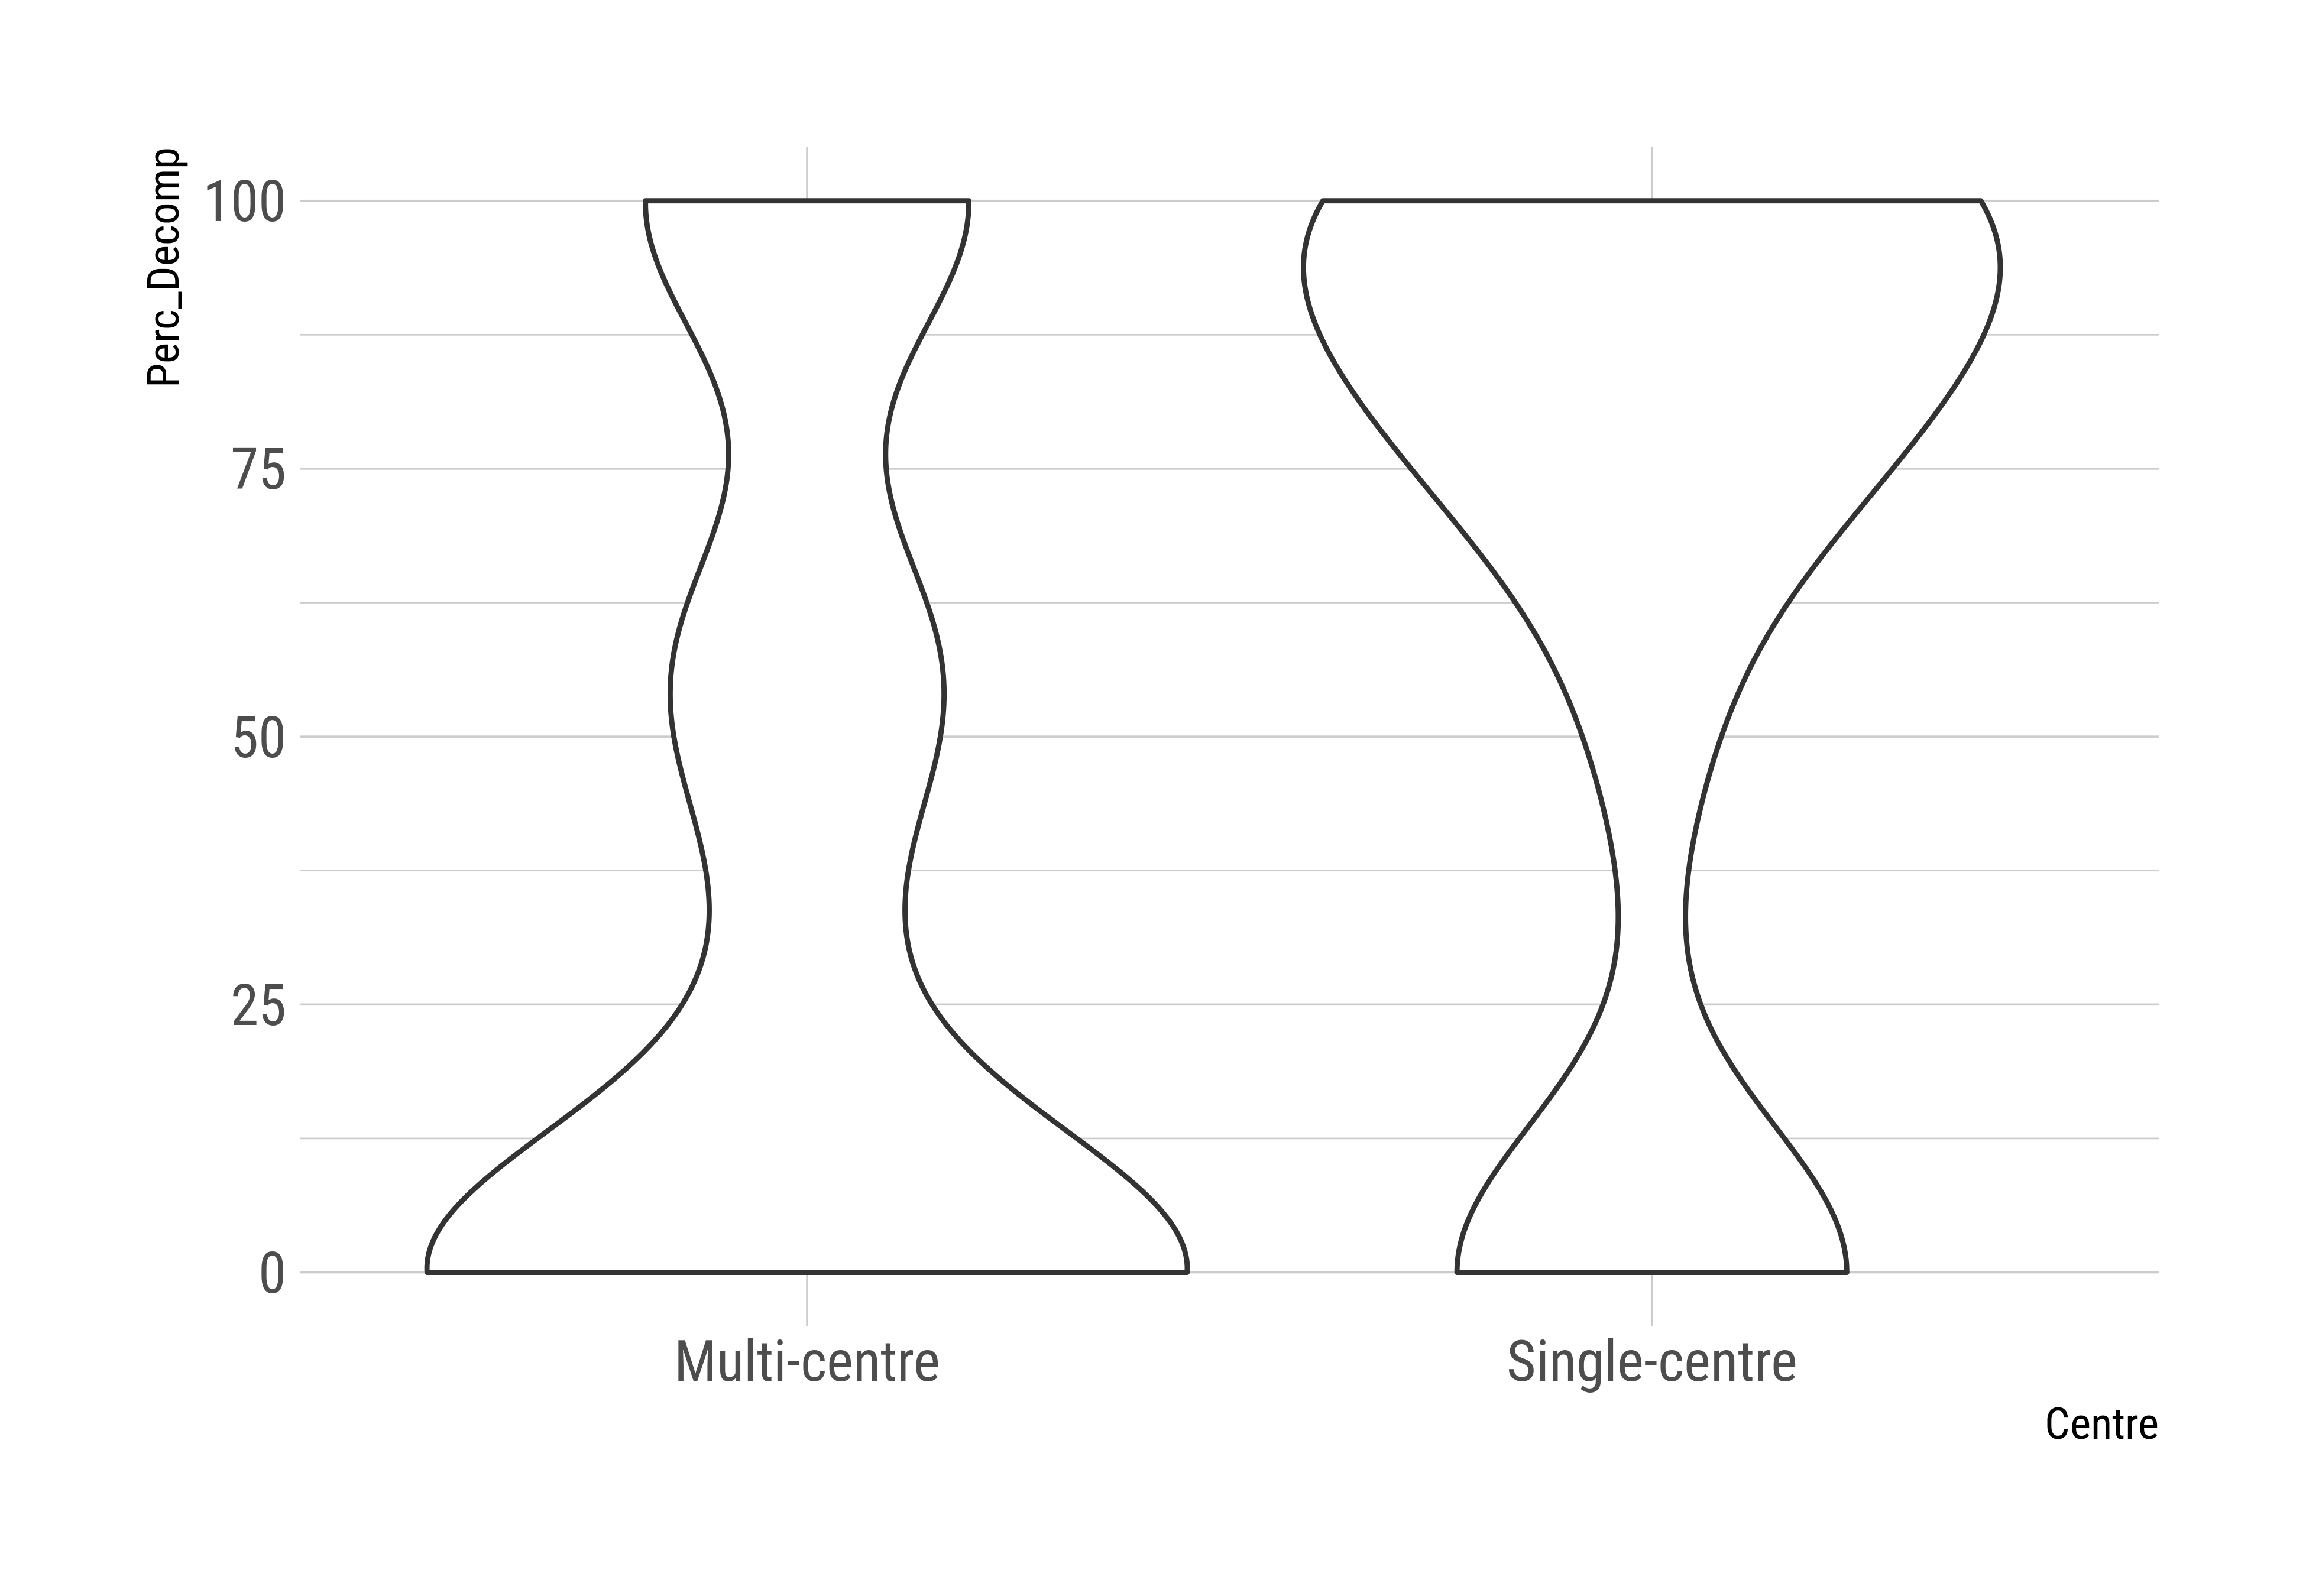
\includegraphics{figures/unnamed-chunk-42-1.png}

\begin{Shaded}
\begin{Highlighting}[]
\FunctionTok{permTS}\NormalTok{(}\AttributeTok{formula=}\NormalTok{Perc\_Decomp }\SpecialCharTok{\textasciitilde{}} \FunctionTok{as.factor}\NormalTok{(Centre), }\AttributeTok{data=}\NormalTok{trt\_wide,}
          \AttributeTok{method=}\StringTok{"exact.mc"}\NormalTok{)}
\end{Highlighting}
\end{Shaded}

\begin{verbatim}
## 
##  Exact Permutation Test Estimated by Monte Carlo
## 
## data:  Perc_Decomp by as.factor(Centre)
## p-value = 0.002
## alternative hypothesis: true mean as.factor(Centre)=Multi-centre - mean as.factor(Centre)=Single-centre is not equal to 0
## sample estimates:
## mean as.factor(Centre)=Multi-centre - mean as.factor(Centre)=Single-centre 
##                                                                  -28.31913 
## 
## p-value estimated from 999 Monte Carlo replications
## 99 percent confidence interval on p-value:
##  0.00000000 0.01057916
\end{verbatim}

Most of the single-centre studies have high proportions of decompensated
patients.

\begin{Shaded}
\begin{Highlighting}[]
\NormalTok{trt\_wide }\SpecialCharTok{\%\textgreater{}\%} 
  \FunctionTok{ggplot}\NormalTok{(}\FunctionTok{aes}\NormalTok{(}\AttributeTok{y=}\NormalTok{Perc\_Alc, }\AttributeTok{x=}\NormalTok{Centre)) }\SpecialCharTok{+} 
  \FunctionTok{geom\_violin}\NormalTok{()}
\end{Highlighting}
\end{Shaded}

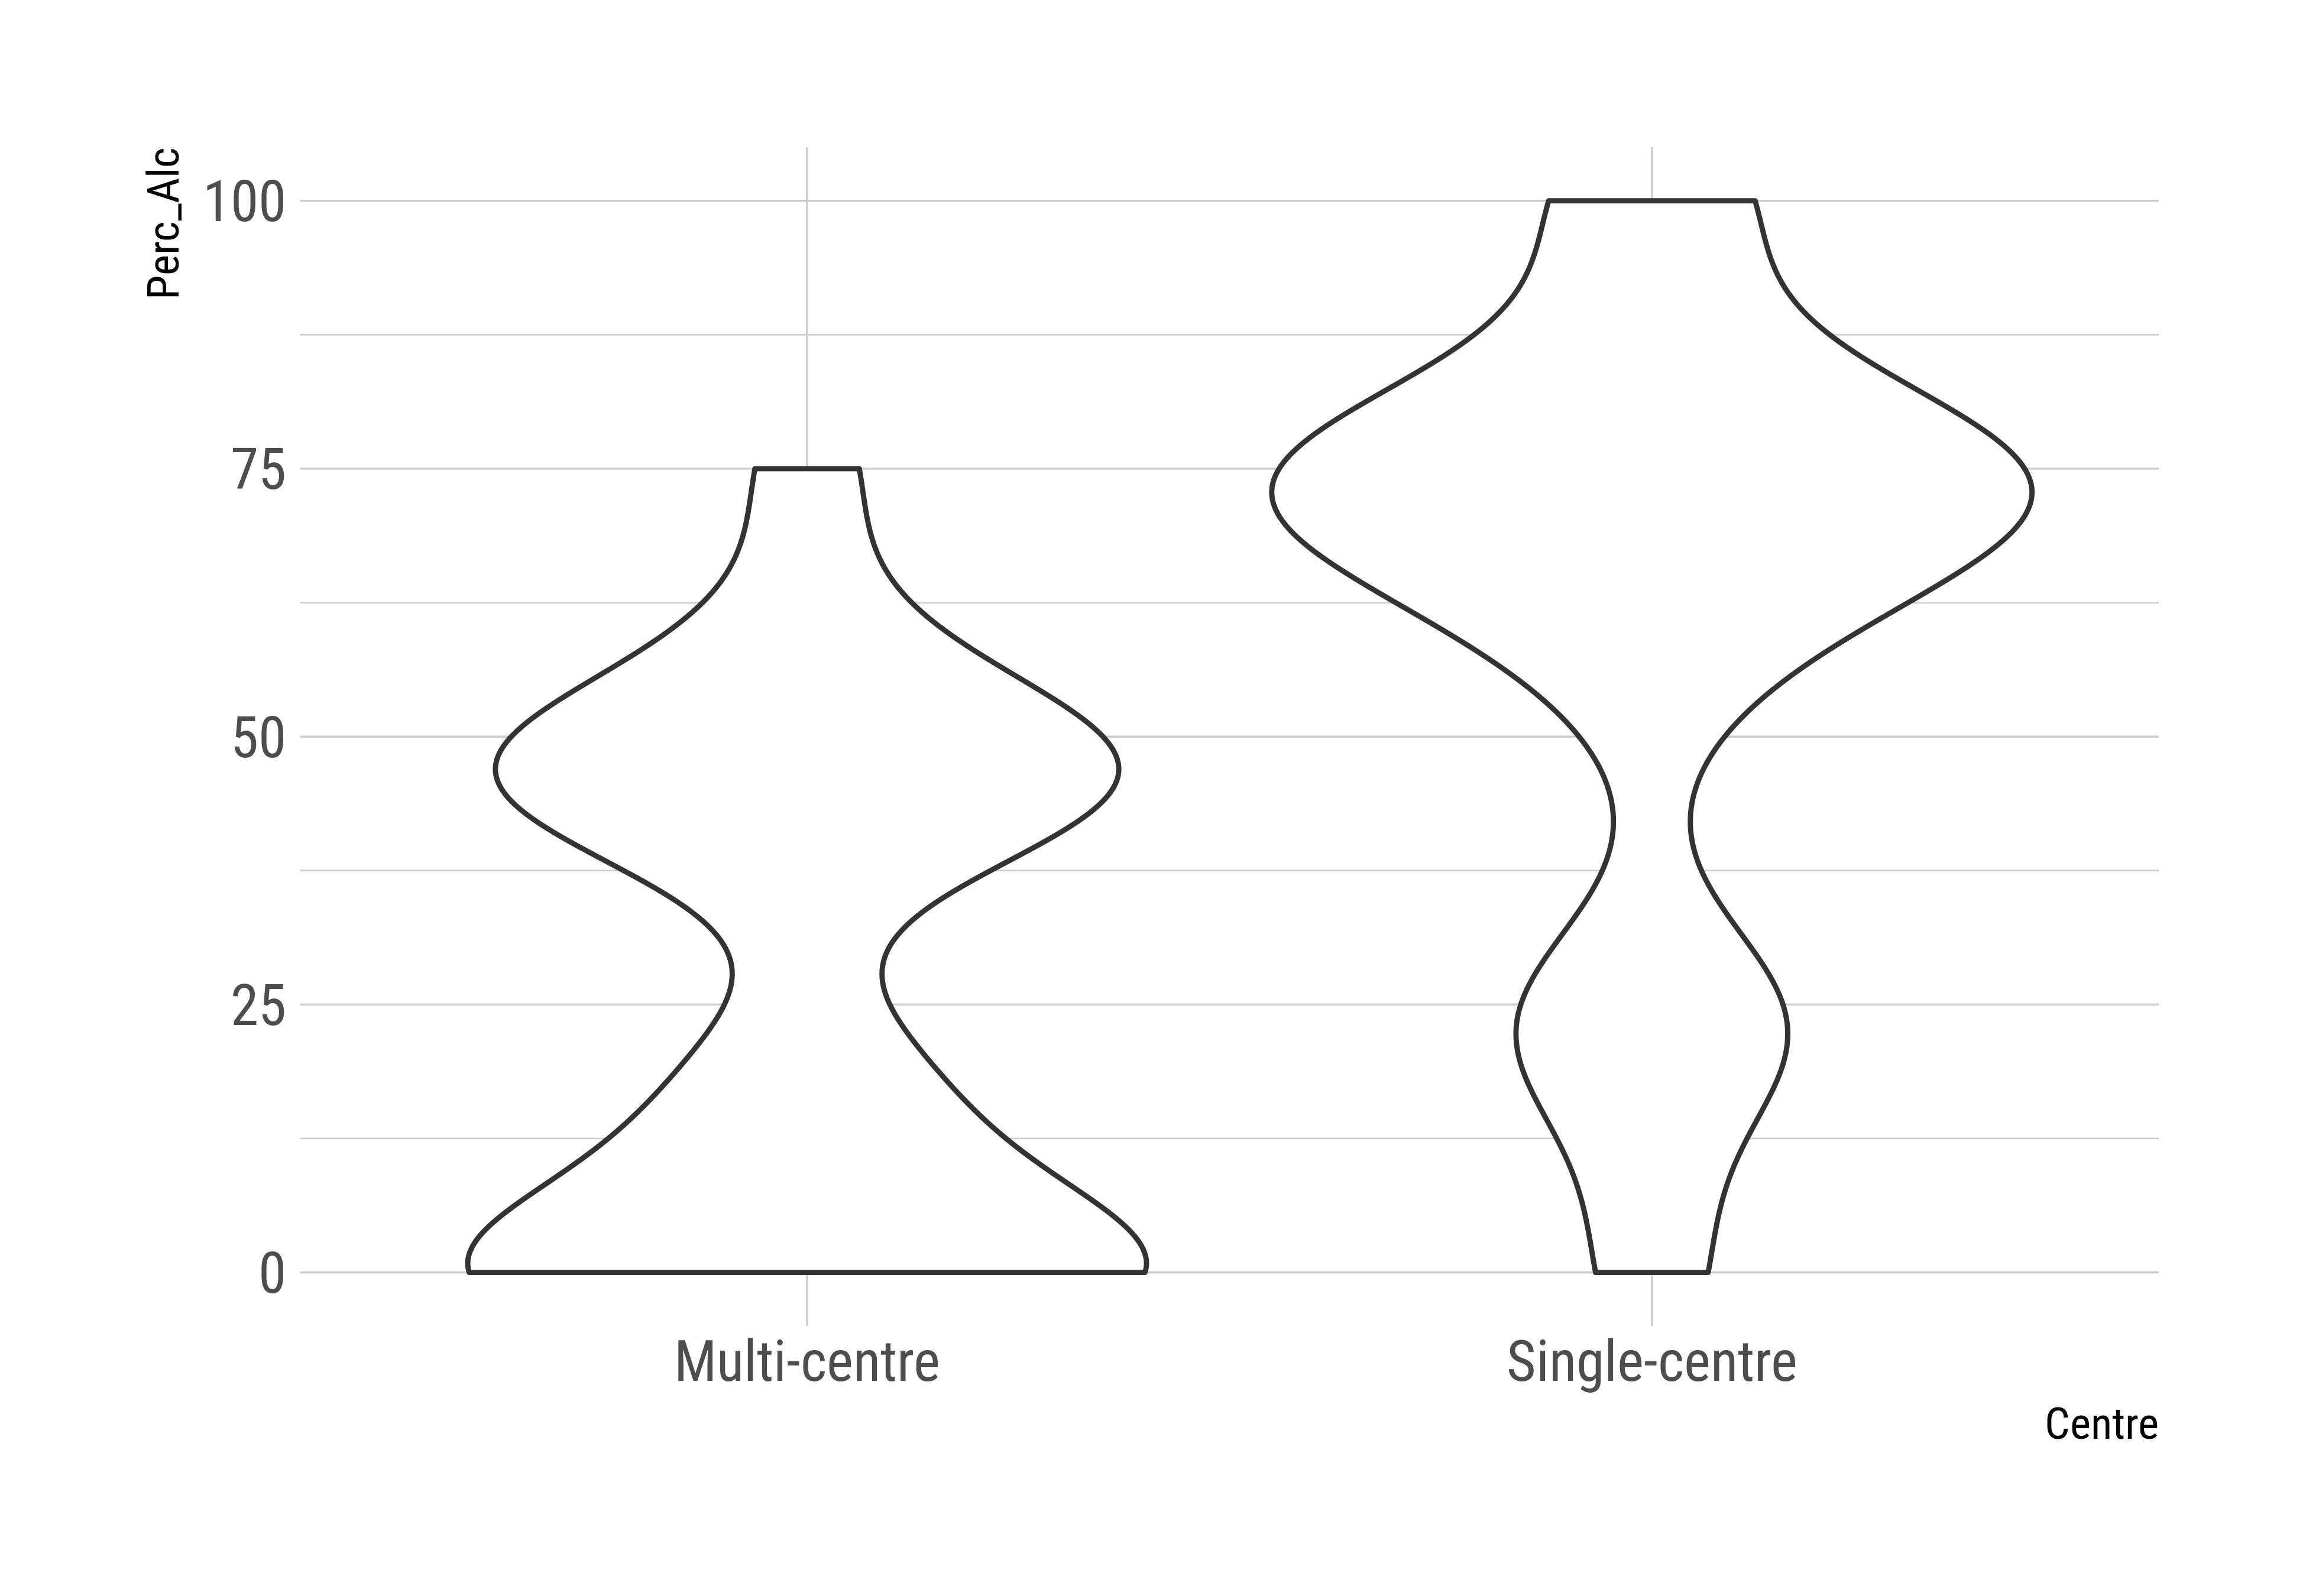
\includegraphics{figures/unnamed-chunk-43-1.png}

\begin{Shaded}
\begin{Highlighting}[]
\FunctionTok{permTS}\NormalTok{(}\AttributeTok{formula=}\NormalTok{Perc\_Alc }\SpecialCharTok{\textasciitilde{}} \FunctionTok{as.factor}\NormalTok{(Centre), }\AttributeTok{data=}\NormalTok{trt\_wide,}
          \AttributeTok{method=}\StringTok{"exact.mc"}\NormalTok{)}
\end{Highlighting}
\end{Shaded}

\begin{verbatim}
## 
##  Exact Permutation Test Estimated by Monte Carlo
## 
## data:  Perc_Alc by as.factor(Centre)
## p-value = 0.002
## alternative hypothesis: true mean as.factor(Centre)=Multi-centre - mean as.factor(Centre)=Single-centre is not equal to 0
## sample estimates:
## mean as.factor(Centre)=Multi-centre - mean as.factor(Centre)=Single-centre 
##                                                                  -34.52329 
## 
## p-value estimated from 999 Monte Carlo replications
## 99 percent confidence interval on p-value:
##  0.00000000 0.01057916
\end{verbatim}

Similarly, most of the single-centre studies have high proportions of
alcoholic patients.

\hypertarget{days}{%
\subsubsection{Days}\label{days}}

Reviewers were surprised at the lack of an effect of the number of days
elapsed. Perhaps this was obscured by not having included the other
confounding factors.

\begin{Shaded}
\begin{Highlighting}[]
\NormalTok{permuco}\SpecialCharTok{::}\FunctionTok{lmperm}\NormalTok{(abschange }\SpecialCharTok{\textasciitilde{}}\NormalTok{ Perc\_Decomp }\SpecialCharTok{+}\NormalTok{ Centre }\SpecialCharTok{+}\NormalTok{ Perc\_Alc }\SpecialCharTok{+}\NormalTok{ Days, }\AttributeTok{data=}\NormalTok{trt\_wide)}
\end{Highlighting}
\end{Shaded}

\begin{verbatim}
## Table of marginal t-test of the betas
## Permutation test using freedman_lane to handle nuisance variables and 5000 permutations.
##                       Estimate Std. Error  t value parametric Pr(>|t|)
## (Intercept)          2.0833441  0.2090856  9.96407           3.545e-20
## Perc_Decomp          0.0178489  0.0034640  5.15263           4.898e-07
## CentreSingle-centre  0.0234628  0.2360917  0.09938           9.209e-01
## Perc_Alc            -0.0262613  0.0052018 -5.04852           8.097e-07
## Days                -0.0007942  0.0007107 -1.11745           2.648e-01
##                     permutation Pr(<t) permutation Pr(>t) permutation Pr(>|t|)
## (Intercept)                                                                   
## Perc_Decomp                     1.0000             0.0002               0.0002
## CentreSingle-centre             0.5348             0.4654               0.9186
## Perc_Alc                        0.0002             1.0000               0.0002
## Days                            0.1308             0.8694               0.2550
\end{verbatim}

This does not appear to be the case!

\hypertarget{mean-value}{%
\subsection{Mean Value}\label{mean-value}}

\hypertarget{absolute-2}{%
\subsubsection{Absolute}\label{absolute-2}}

\begin{Shaded}
\begin{Highlighting}[]
\NormalTok{permuco}\SpecialCharTok{::}\FunctionTok{lmperm}\NormalTok{(abschange }\SpecialCharTok{\textasciitilde{}}\NormalTok{ meanval }\SpecialCharTok{+}\NormalTok{ Perc\_Decomp, }\AttributeTok{data=}\NormalTok{trt\_wide)}
\end{Highlighting}
\end{Shaded}

\begin{verbatim}
## Table of marginal t-test of the betas
## Permutation test using freedman_lane to handle nuisance variables and 5000 permutations.
##             Estimate Std. Error t value parametric Pr(>|t|) permutation Pr(<t)
## (Intercept) 1.085870   0.422931   2.567             0.01077                   
## meanval     0.025623   0.024418   1.049             0.29494             0.8470
## Perc_Decomp 0.004602   0.002401   1.917             0.05630             0.9774
##             permutation Pr(>t) permutation Pr(>|t|)
## (Intercept)                                        
## meanval                 0.1532                0.299
## Perc_Decomp             0.0228                0.054
\end{verbatim}

\begin{Shaded}
\begin{Highlighting}[]
\FunctionTok{permTREND}\NormalTok{(}\AttributeTok{formula=}\NormalTok{abschange }\SpecialCharTok{\textasciitilde{}}\NormalTok{ meanval, }\AttributeTok{data=}\NormalTok{trt\_wide\_c,}
          \AttributeTok{method=}\StringTok{"exact.mc"}\NormalTok{)}
\end{Highlighting}
\end{Shaded}

\begin{verbatim}
## 
##  Exact Permutation Test Estimated by Monte Carlo
## 
## data:  x and y
## p-value = 0.654
## alternative hypothesis: true correlation of x and y is not equal to 0
## sample estimates:
## correlation of x and y 
##            -0.04578405 
## 
## p-value estimated from 999 Monte Carlo replications
## 99 percent confidence interval on p-value:
##  0.5770505 0.7316143
\end{verbatim}

\begin{Shaded}
\begin{Highlighting}[]
\FunctionTok{permTREND}\NormalTok{(}\AttributeTok{formula=}\NormalTok{abschange }\SpecialCharTok{\textasciitilde{}}\NormalTok{ meanval, }\AttributeTok{data=}\NormalTok{trt\_wide\_dc,}
          \AttributeTok{method=}\StringTok{"exact.mc"}\NormalTok{)}
\end{Highlighting}
\end{Shaded}

\begin{verbatim}
## 
##  Exact Permutation Test Estimated by Monte Carlo
## 
## data:  x and y
## p-value = 0.114
## alternative hypothesis: true correlation of x and y is not equal to 0
## sample estimates:
## correlation of x and y 
##              0.1302787 
## 
## p-value estimated from 999 Monte Carlo replications
## 99 percent confidence interval on p-value:
##  0.07792884 0.15503144
\end{verbatim}

\begin{Shaded}
\begin{Highlighting}[]
\NormalTok{meanv\_abs\_plot }\OtherTok{\textless{}{-}}\NormalTok{ trt\_wide }\SpecialCharTok{\%\textgreater{}\%} 
  \FunctionTok{mutate}\NormalTok{(}\AttributeTok{abschange\_dccorr =} \FunctionTok{correct\_for\_decomp}\NormalTok{(abschange }\SpecialCharTok{\textasciitilde{}}\NormalTok{ meanval }\SpecialCharTok{+}\NormalTok{ Perc\_Decomp)) }\SpecialCharTok{\%\textgreater{}\%} 
  \FunctionTok{ggplot}\NormalTok{(}\FunctionTok{aes}\NormalTok{(}\AttributeTok{x=}\NormalTok{meanval, }\AttributeTok{y=}\NormalTok{abschange\_dccorr)) }\SpecialCharTok{+}
  \FunctionTok{geom\_point}\NormalTok{(}\FunctionTok{aes}\NormalTok{(}\AttributeTok{colour=}\NormalTok{Study, }\AttributeTok{group=}\NormalTok{Study), }\AttributeTok{alpha=}\FloatTok{0.4}\NormalTok{) }\SpecialCharTok{+}
  \FunctionTok{guides}\NormalTok{(}\AttributeTok{colour=}\ConstantTok{FALSE}\NormalTok{) }\SpecialCharTok{+} 
  \FunctionTok{geom\_smooth}\NormalTok{(}\AttributeTok{method=}\StringTok{"lm"}\NormalTok{, }\AttributeTok{se=}\ConstantTok{FALSE}\NormalTok{) }\SpecialCharTok{+}
  \FunctionTok{labs}\NormalTok{(}\AttributeTok{y=}\StringTok{"Absolute Change (mmHg)}\SpecialCharTok{\textbackslash{}n}\StringTok{(after correction for Decompensated Percentage)"}\NormalTok{,}
       \AttributeTok{x=}\StringTok{"Mean Value across Measurements (mmHg)"}\NormalTok{)}

\NormalTok{meanv\_abs\_plot}
\end{Highlighting}
\end{Shaded}

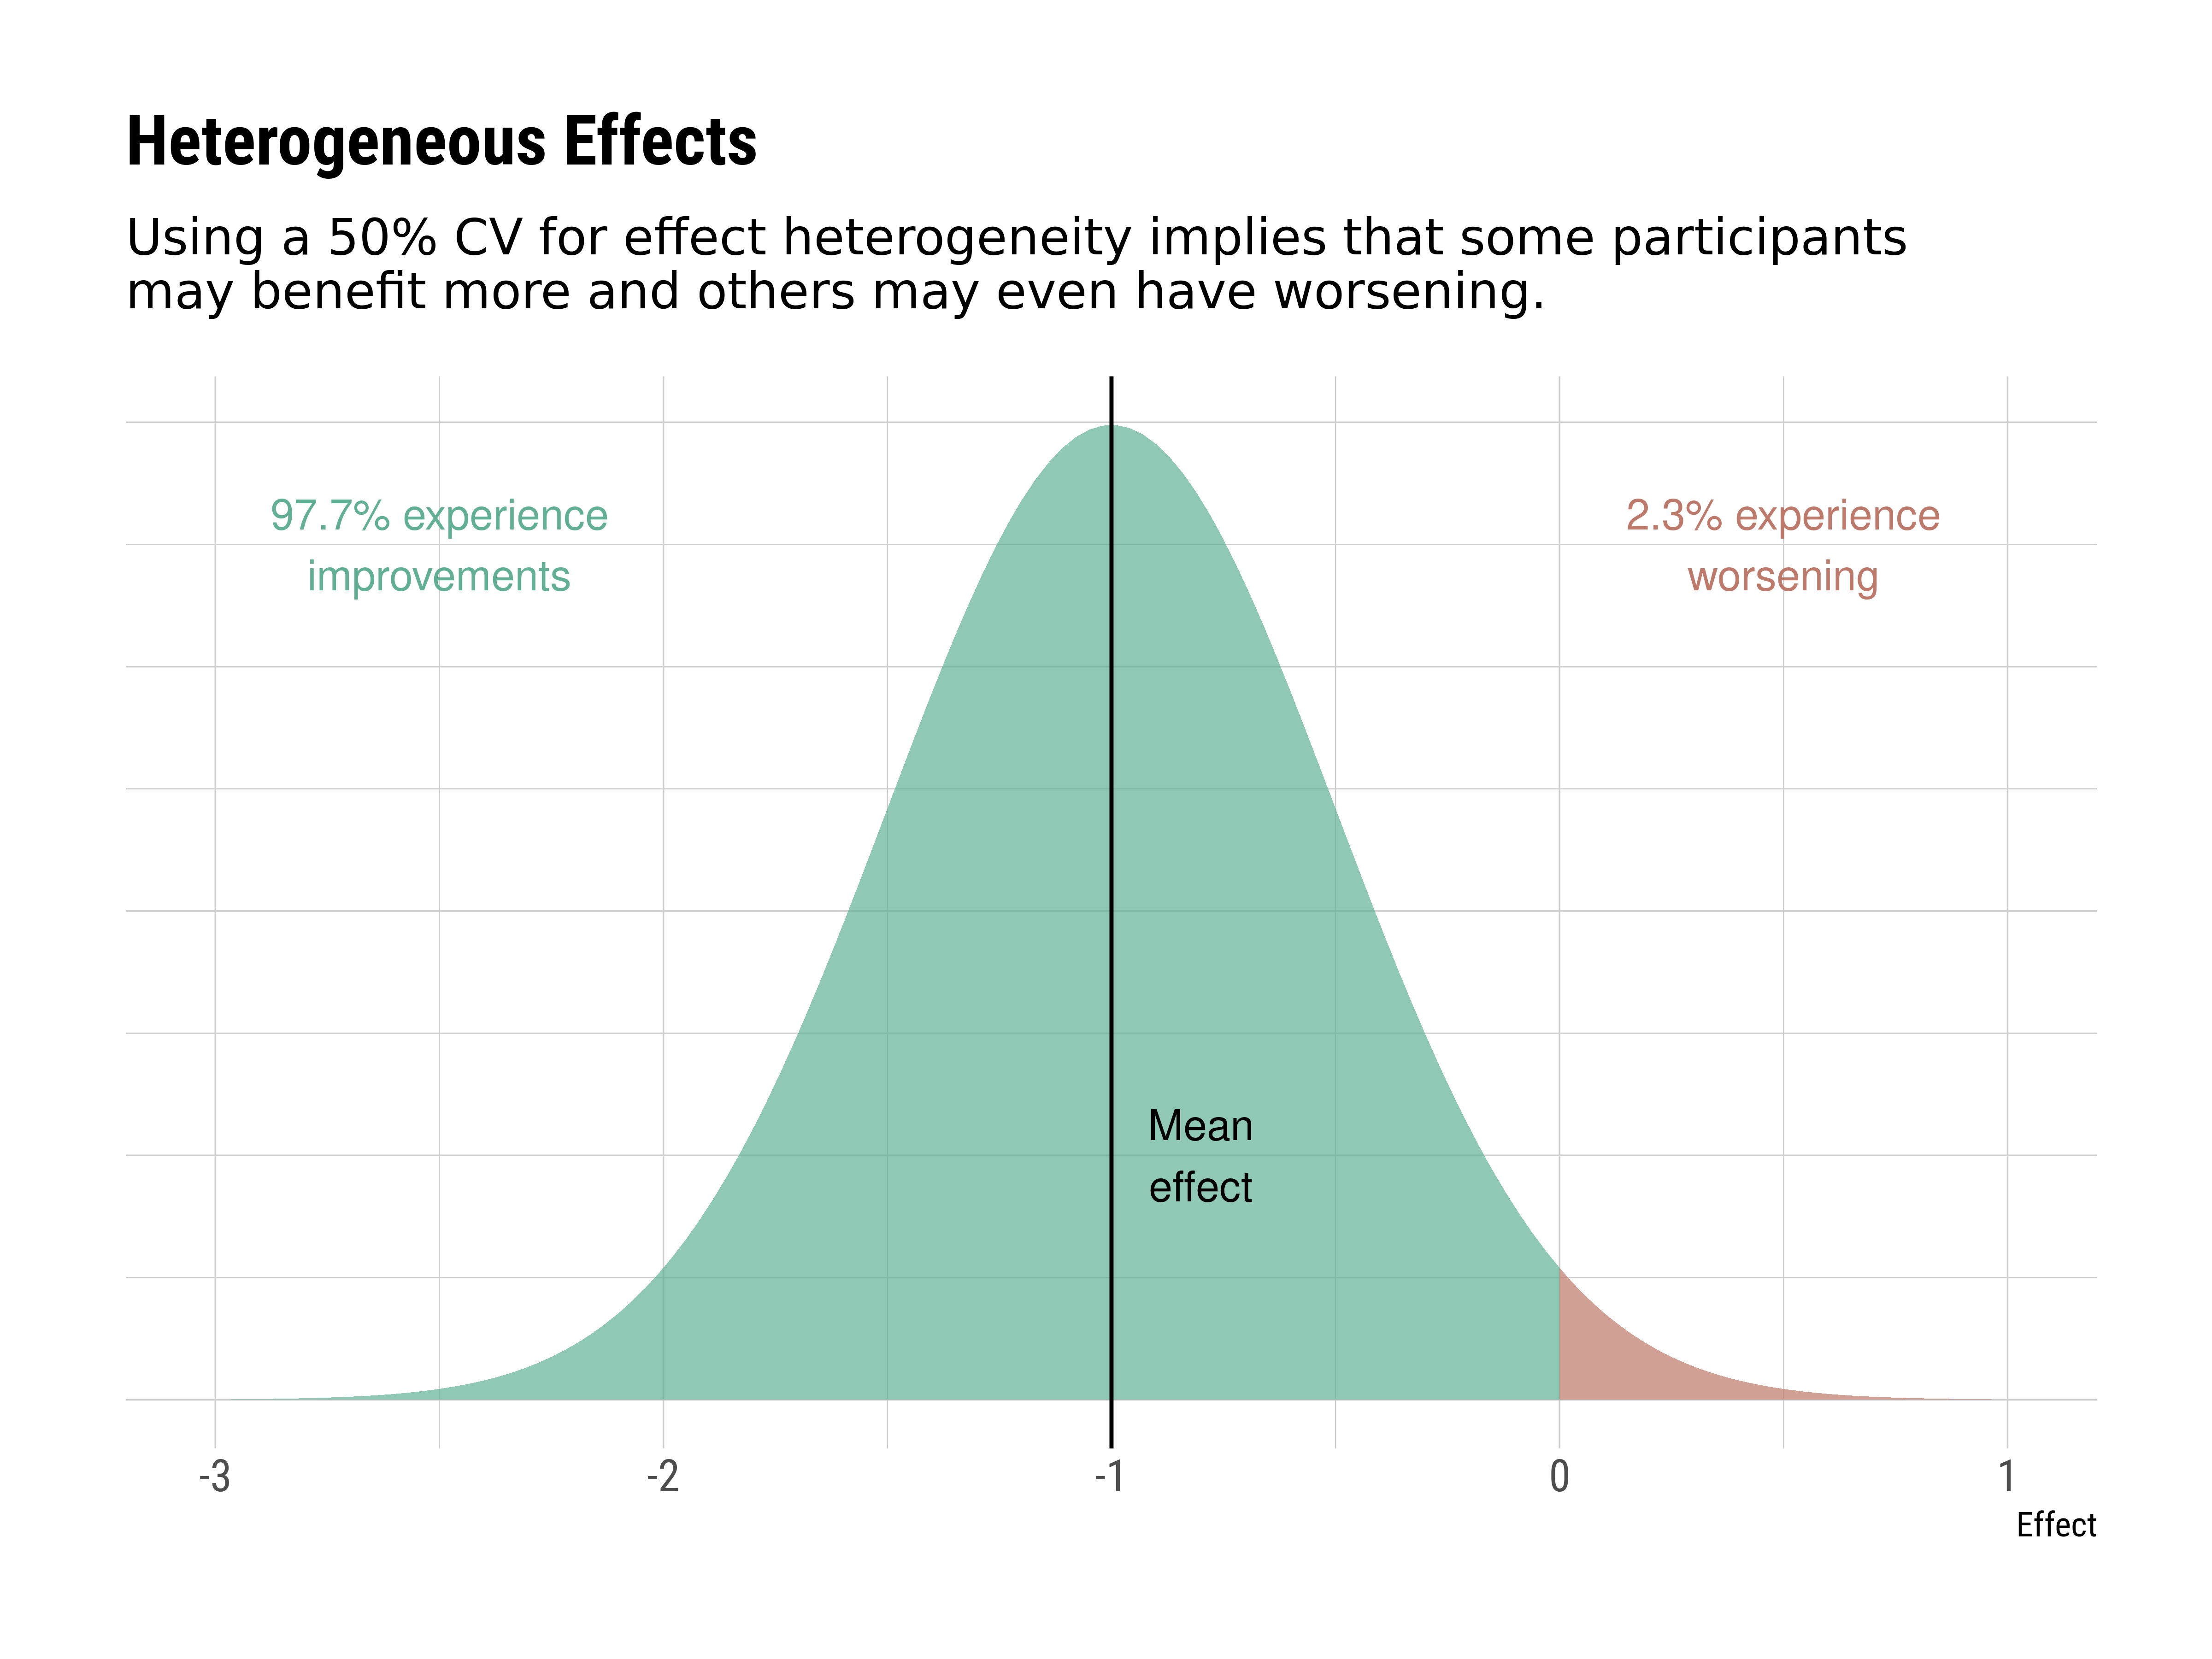
\includegraphics{figures/unnamed-chunk-46-1.png}

\hypertarget{signed-1}{%
\subsubsection{Signed}\label{signed-1}}

\begin{Shaded}
\begin{Highlighting}[]
\NormalTok{meanv\_sign }\OtherTok{\textless{}{-}} \FunctionTok{lmer}\NormalTok{(change }\SpecialCharTok{\textasciitilde{}}\NormalTok{ meanval }\SpecialCharTok{+}\NormalTok{ Perc\_Decomp }\SpecialCharTok{+}\NormalTok{ (}\DecValTok{1} \SpecialCharTok{|}\NormalTok{ Study), }\AttributeTok{data =}\NormalTok{ trt\_wide)}
\FunctionTok{summary}\NormalTok{(meanv\_sign)}
\end{Highlighting}
\end{Shaded}

\begin{verbatim}
## Linear mixed model fit by REML. t-tests use Satterthwaite's method [
## lmerModLmerTest]
## Formula: change ~ meanval + Perc_Decomp + (1 | Study)
##    Data: trt_wide
## 
## REML criterion at convergence: 1304
## 
## Scaled residuals: 
##     Min      1Q  Median      3Q     Max 
## -4.8083 -0.6359  0.0657  0.5932  3.9860 
## 
## Random effects:
##  Groups   Name        Variance Std.Dev.
##  Study    (Intercept) 0.4263   0.6529  
##  Residual             5.5354   2.3527  
## Number of obs: 281, groups:  Study, 21
## 
## Fixed effects:
##               Estimate Std. Error         df t value Pr(>|t|)    
## (Intercept)  -1.773365   0.658135  70.196412  -2.695 0.008813 ** 
## meanval       0.125777   0.034937 258.265538   3.600 0.000381 ***
## Perc_Decomp  -0.007595   0.004939  10.005645  -1.538 0.155110    
## ---
## Signif. codes:  0 '***' 0.001 '**' 0.01 '*' 0.05 '.' 0.1 ' ' 1
## 
## Correlation of Fixed Effects:
##             (Intr) meanvl
## meanval     -0.860       
## Perc_Decomp -0.301 -0.110
\end{verbatim}

\begin{Shaded}
\begin{Highlighting}[]
\NormalTok{meanv\_sign\_nocorr }\OtherTok{\textless{}{-}} \FunctionTok{lmer}\NormalTok{(change }\SpecialCharTok{\textasciitilde{}}\NormalTok{ meanval }\SpecialCharTok{+}\NormalTok{ (}\DecValTok{1} \SpecialCharTok{|}\NormalTok{ Study), }\AttributeTok{data =}\NormalTok{ trt\_wide)}
\FunctionTok{summary}\NormalTok{(meanv\_sign\_nocorr)}
\end{Highlighting}
\end{Shaded}

\begin{verbatim}
## Linear mixed model fit by REML. t-tests use Satterthwaite's method [
## lmerModLmerTest]
## Formula: change ~ meanval + (1 | Study)
##    Data: trt_wide
## 
## REML criterion at convergence: 1297.6
## 
## Scaled residuals: 
##     Min      1Q  Median      3Q     Max 
## -4.8493 -0.6062  0.0470  0.5689  3.9289 
## 
## Random effects:
##  Groups   Name        Variance Std.Dev.
##  Study    (Intercept) 0.505    0.7106  
##  Residual             5.530    2.3515  
## Number of obs: 281, groups:  Study, 21
## 
## Fixed effects:
##             Estimate Std. Error       df t value Pr(>|t|)    
## (Intercept)  -2.1062     0.6338 161.0550  -3.323 0.001102 ** 
## meanval       0.1215     0.0349 258.7515   3.481 0.000586 ***
## ---
## Signif. codes:  0 '***' 0.001 '**' 0.01 '*' 0.05 '.' 0.1 ' ' 1
## 
## Correlation of Fixed Effects:
##         (Intr)
## meanval -0.938
\end{verbatim}

\begin{Shaded}
\begin{Highlighting}[]
\NormalTok{meanv\_sign\_c }\OtherTok{\textless{}{-}} \FunctionTok{lmer}\NormalTok{(change }\SpecialCharTok{\textasciitilde{}}\NormalTok{ meanval }\SpecialCharTok{+}\NormalTok{ (}\DecValTok{1} \SpecialCharTok{|}\NormalTok{ Study), }\AttributeTok{data =}\NormalTok{ trt\_wide\_c)}
\FunctionTok{summary}\NormalTok{(meanv\_sign\_c)}
\end{Highlighting}
\end{Shaded}

\begin{verbatim}
## Linear mixed model fit by REML. t-tests use Satterthwaite's method [
## lmerModLmerTest]
## Formula: change ~ meanval + (1 | Study)
##    Data: trt_wide_c
## 
## REML criterion at convergence: 505.3
## 
## Scaled residuals: 
##      Min       1Q   Median       3Q      Max 
## -1.95680 -0.66000 -0.09292  0.72674  2.50831 
## 
## Random effects:
##  Groups   Name        Variance Std.Dev.
##  Study    (Intercept) 0.1447   0.3804  
##  Residual             4.5220   2.1265  
## Number of obs: 115, groups:  Study, 7
## 
## Fixed effects:
##              Estimate Std. Error        df t value Pr(>|t|)  
## (Intercept)  -1.82528    0.95247  64.26834  -1.916   0.0598 .
## meanval       0.12622    0.05556 102.76959   2.272   0.0252 *
## ---
## Signif. codes:  0 '***' 0.001 '**' 0.01 '*' 0.05 '.' 0.1 ' ' 1
## 
## Correlation of Fixed Effects:
##         (Intr)
## meanval -0.961
\end{verbatim}

\begin{Shaded}
\begin{Highlighting}[]
\NormalTok{meanv\_sign\_dc }\OtherTok{\textless{}{-}} \FunctionTok{lmer}\NormalTok{(change }\SpecialCharTok{\textasciitilde{}}\NormalTok{ meanval }\SpecialCharTok{+}\NormalTok{ (}\DecValTok{1} \SpecialCharTok{|}\NormalTok{ Study), }\AttributeTok{data =}\NormalTok{ trt\_wide\_dc)}
\FunctionTok{summary}\NormalTok{(meanv\_sign\_dc)}
\end{Highlighting}
\end{Shaded}

\begin{verbatim}
## Linear mixed model fit by REML. t-tests use Satterthwaite's method [
## lmerModLmerTest]
## Formula: change ~ meanval + (1 | Study)
##    Data: trt_wide_dc
## 
## REML criterion at convergence: 789.3
## 
## Scaled residuals: 
##     Min      1Q  Median      3Q     Max 
## -4.4469 -0.5597  0.1251  0.5181  3.7263 
## 
## Random effects:
##  Groups   Name        Variance Std.Dev.
##  Study    (Intercept) 0.6818   0.8257  
##  Residual             6.2470   2.4994  
## Number of obs: 166, groups:  Study, 14
## 
## Fixed effects:
##              Estimate Std. Error        df t value Pr(>|t|)   
## (Intercept)  -2.33529    0.83332 100.93794  -2.802  0.00608 **
## meanval       0.12351    0.04499 153.92550   2.745  0.00677 **
## ---
## Signif. codes:  0 '***' 0.001 '**' 0.01 '*' 0.05 '.' 0.1 ' ' 1
## 
## Correlation of Fixed Effects:
##         (Intr)
## meanval -0.932
\end{verbatim}

\begin{Shaded}
\begin{Highlighting}[]
\NormalTok{correct\_for\_decomp\_lmer }\OtherTok{\textless{}{-}} \ControlFlowTok{function}\NormalTok{(formula) \{}
  
\NormalTok{  formula }\OtherTok{\textless{}{-}} \FunctionTok{as.formula}\NormalTok{(formula)}
  
\NormalTok{  coefficients }\OtherTok{\textless{}{-}} \FunctionTok{fixef}\NormalTok{(}\FunctionTok{lmer}\NormalTok{(formula, }\AttributeTok{data=}\NormalTok{trt\_wide))}

\NormalTok{  predicted }\OtherTok{\textless{}{-}} \FunctionTok{as.character}\NormalTok{(formula[}\DecValTok{2}\NormalTok{])}
  
\NormalTok{  after\_decomp\_corr }\OtherTok{\textless{}{-}}\NormalTok{ trt\_wide[[predicted]] }\SpecialCharTok{{-}} 
\NormalTok{    trt\_wide[[}\StringTok{"Perc\_Decomp"}\NormalTok{]] }\SpecialCharTok{*}\NormalTok{ coefficients[}\FunctionTok{which}\NormalTok{(}\FunctionTok{names}\NormalTok{(coefficients)}\SpecialCharTok{==}\StringTok{"Perc\_Decomp"}\NormalTok{)]}
  
  \FunctionTok{return}\NormalTok{(after\_decomp\_corr)}
  
\NormalTok{\}}


\NormalTok{meanv\_signed\_plot }\OtherTok{\textless{}{-}}\NormalTok{ trt\_wide }\SpecialCharTok{\%\textgreater{}\%} 
  \FunctionTok{mutate}\NormalTok{(}\AttributeTok{change\_dccorr =} \FunctionTok{correct\_for\_decomp\_lmer}\NormalTok{(}\StringTok{"change \textasciitilde{} meanval + Perc\_Decomp + (1 | Study)"}\NormalTok{)) }\SpecialCharTok{\%\textgreater{}\%} 
  \FunctionTok{ggplot}\NormalTok{(}\FunctionTok{aes}\NormalTok{(}\AttributeTok{x=}\NormalTok{meanval, }\AttributeTok{y=}\NormalTok{change\_dccorr)) }\SpecialCharTok{+}
  \FunctionTok{geom\_jitter}\NormalTok{(}\FunctionTok{aes}\NormalTok{(}\AttributeTok{colour=}\NormalTok{Study, }\AttributeTok{group=}\NormalTok{Study), }\AttributeTok{alpha=}\FloatTok{0.4}\NormalTok{, }\AttributeTok{height =} \FloatTok{0.2}\NormalTok{) }\SpecialCharTok{+}
  \FunctionTok{guides}\NormalTok{(}\AttributeTok{colour=}\ConstantTok{FALSE}\NormalTok{) }\SpecialCharTok{+} 
  \FunctionTok{geom\_smooth}\NormalTok{(}\AttributeTok{method=}\StringTok{"lm"}\NormalTok{, }\AttributeTok{se=}\ConstantTok{FALSE}\NormalTok{) }\SpecialCharTok{+}
  \FunctionTok{labs}\NormalTok{(}\AttributeTok{y=}\StringTok{"Signed Change (mmHg)}\SpecialCharTok{\textbackslash{}n}\StringTok{(after correction for Decompensated Percentage)"}\NormalTok{,}
       \AttributeTok{x=}\StringTok{"Mean Value across Measurements (mmHg)"}\NormalTok{)}

\NormalTok{meanv\_signed\_plot}
\end{Highlighting}
\end{Shaded}

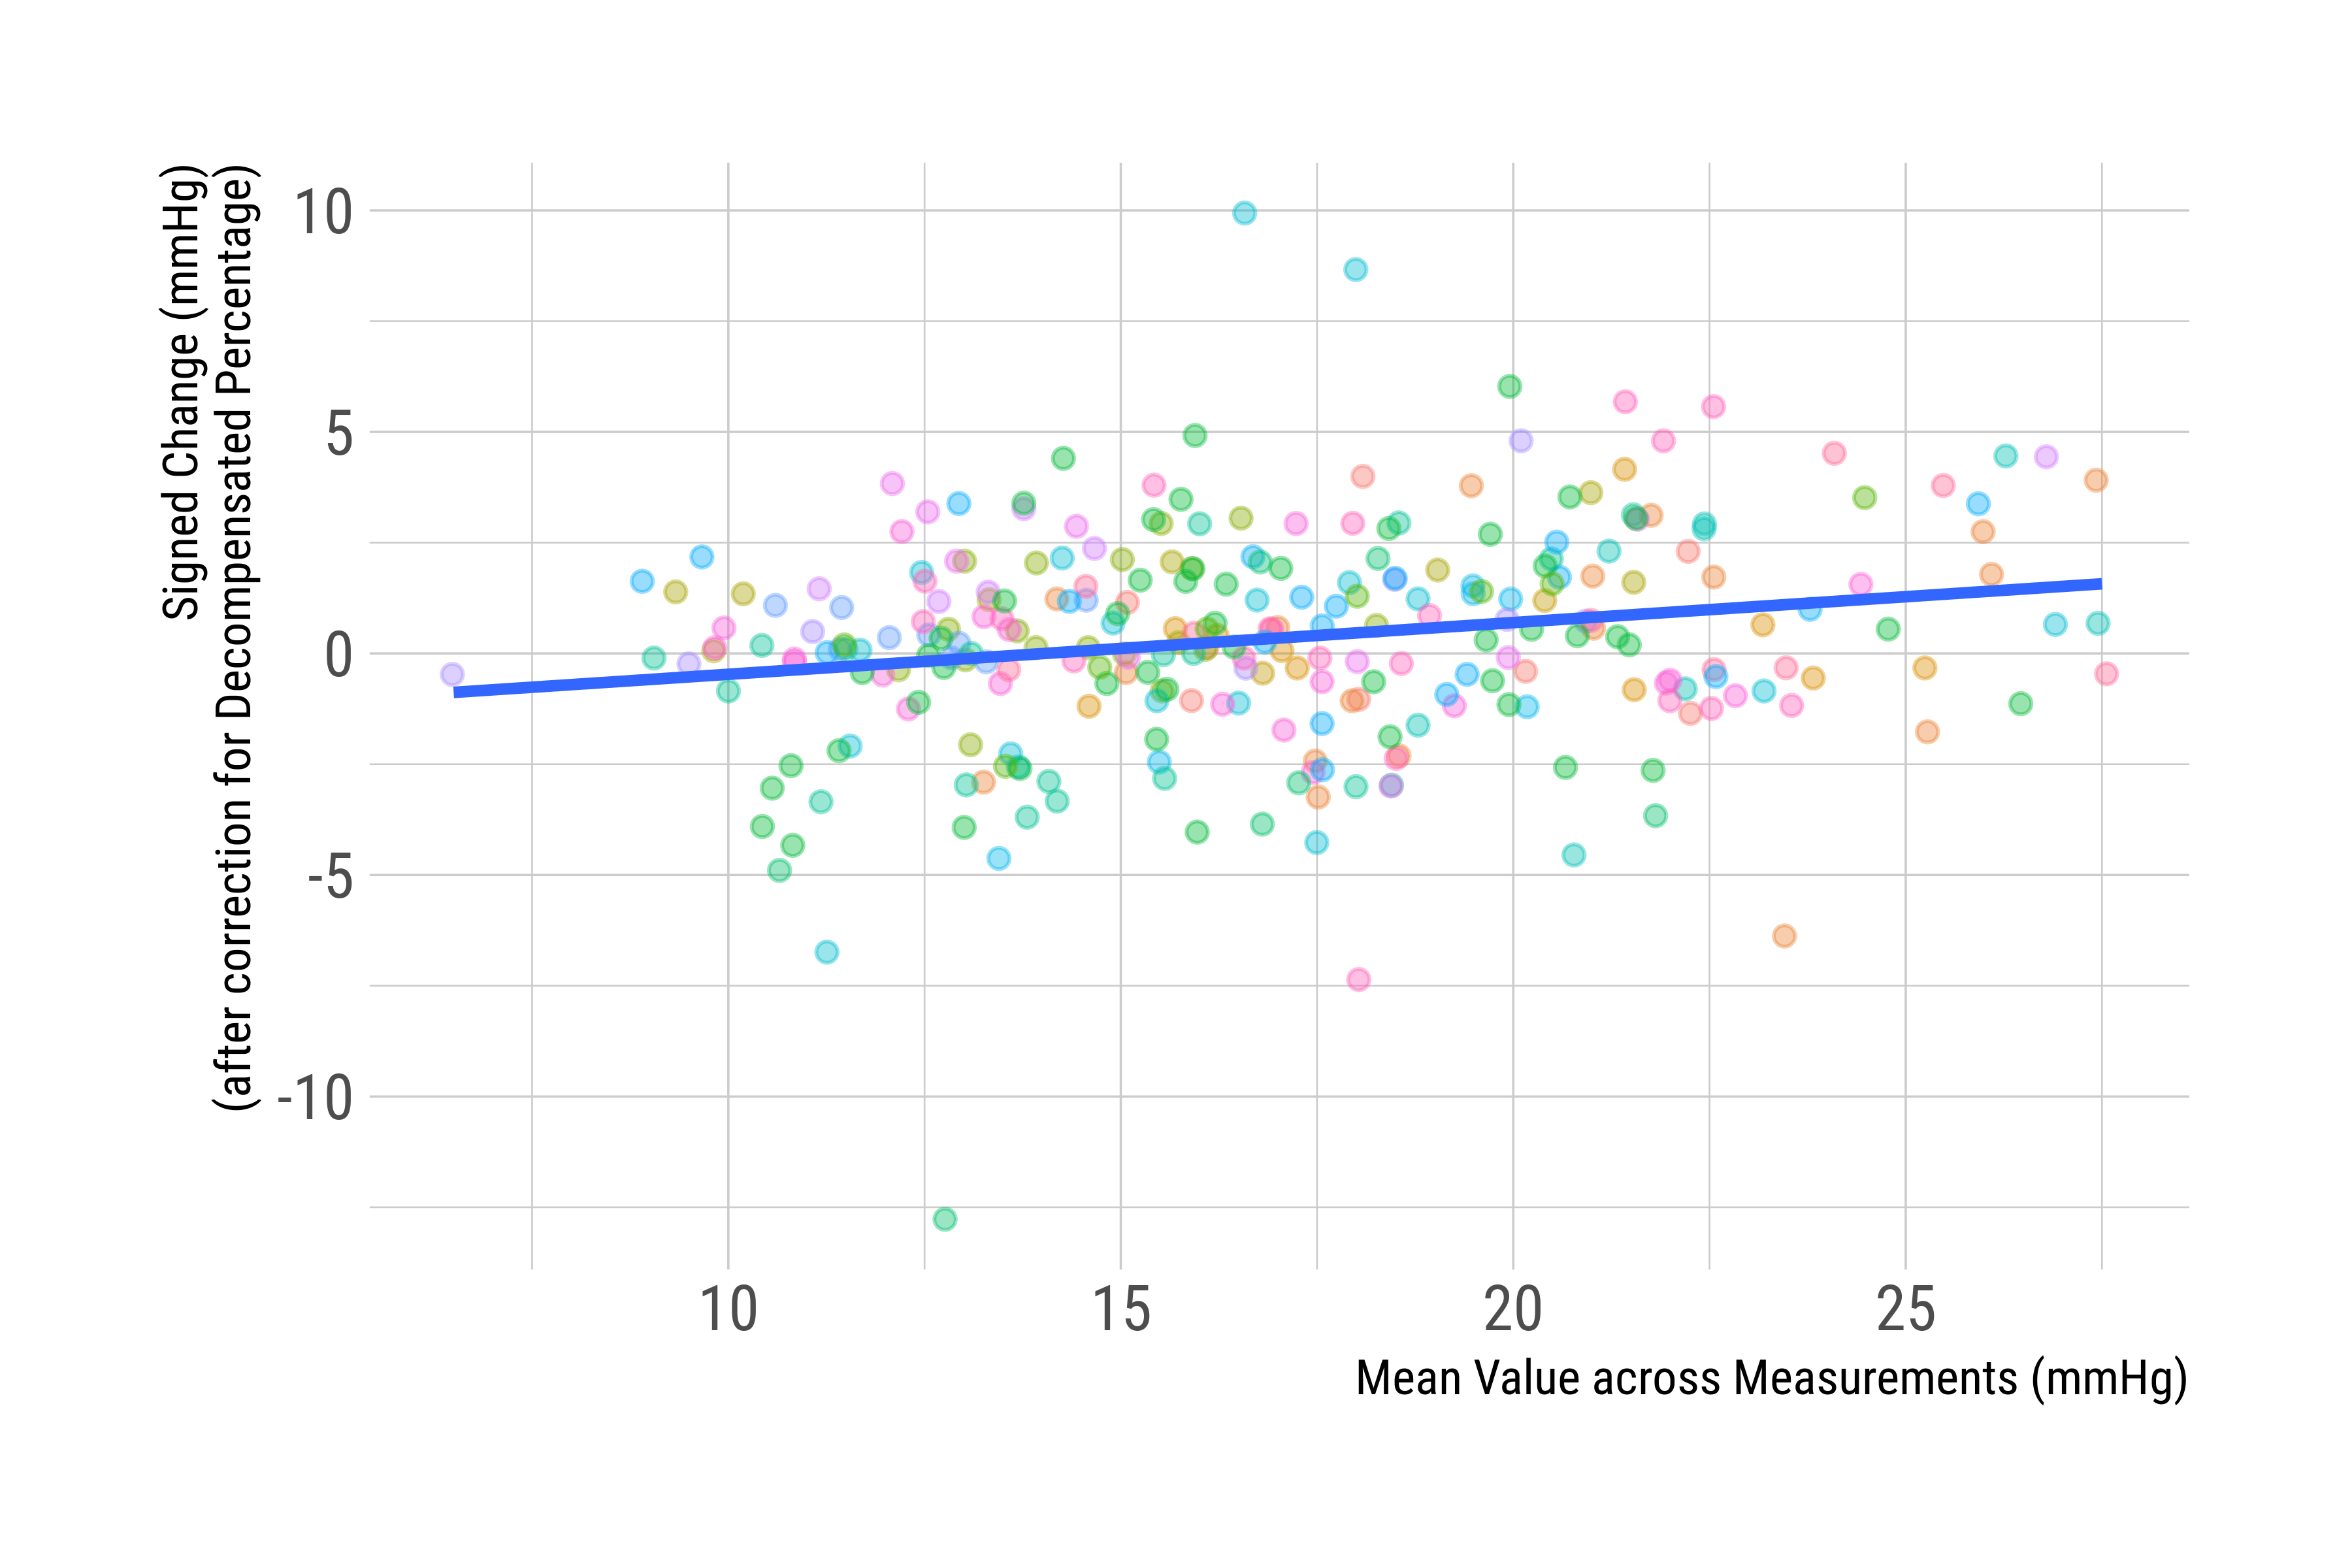
\includegraphics{figures/unnamed-chunk-48-1.png}

\begin{Shaded}
\begin{Highlighting}[]
\NormalTok{meanv\_signed\_plot\_nocorr }\OtherTok{\textless{}{-}} \FunctionTok{ggplot}\NormalTok{(}\AttributeTok{data=}\NormalTok{trt\_wide, }\FunctionTok{aes}\NormalTok{(}\AttributeTok{x=}\NormalTok{meanval, }\AttributeTok{y=}\NormalTok{change)) }\SpecialCharTok{+}
  \FunctionTok{geom\_jitter}\NormalTok{(}\FunctionTok{aes}\NormalTok{(}\AttributeTok{colour=}\NormalTok{Study, }\AttributeTok{group=}\NormalTok{Study), }\AttributeTok{alpha=}\FloatTok{0.4}\NormalTok{, }\AttributeTok{height =} \FloatTok{0.2}\NormalTok{) }\SpecialCharTok{+}
  \FunctionTok{guides}\NormalTok{(}\AttributeTok{colour=}\ConstantTok{FALSE}\NormalTok{) }\SpecialCharTok{+} 
  \FunctionTok{geom\_smooth}\NormalTok{(}\AttributeTok{method=}\StringTok{"lm"}\NormalTok{, }\AttributeTok{se=}\ConstantTok{FALSE}\NormalTok{) }\SpecialCharTok{+}
  \FunctionTok{labs}\NormalTok{(}\AttributeTok{y=}\StringTok{"Signed Change (mmHg)}\SpecialCharTok{\textbackslash{}n}\StringTok{(jittered slightly to avoid overlap)"}\NormalTok{,}
       \AttributeTok{x=}\StringTok{"Mean Value across Measurements (mmHg)"}\NormalTok{)}

\NormalTok{meanv\_signed\_plot\_nocorr}
\end{Highlighting}
\end{Shaded}

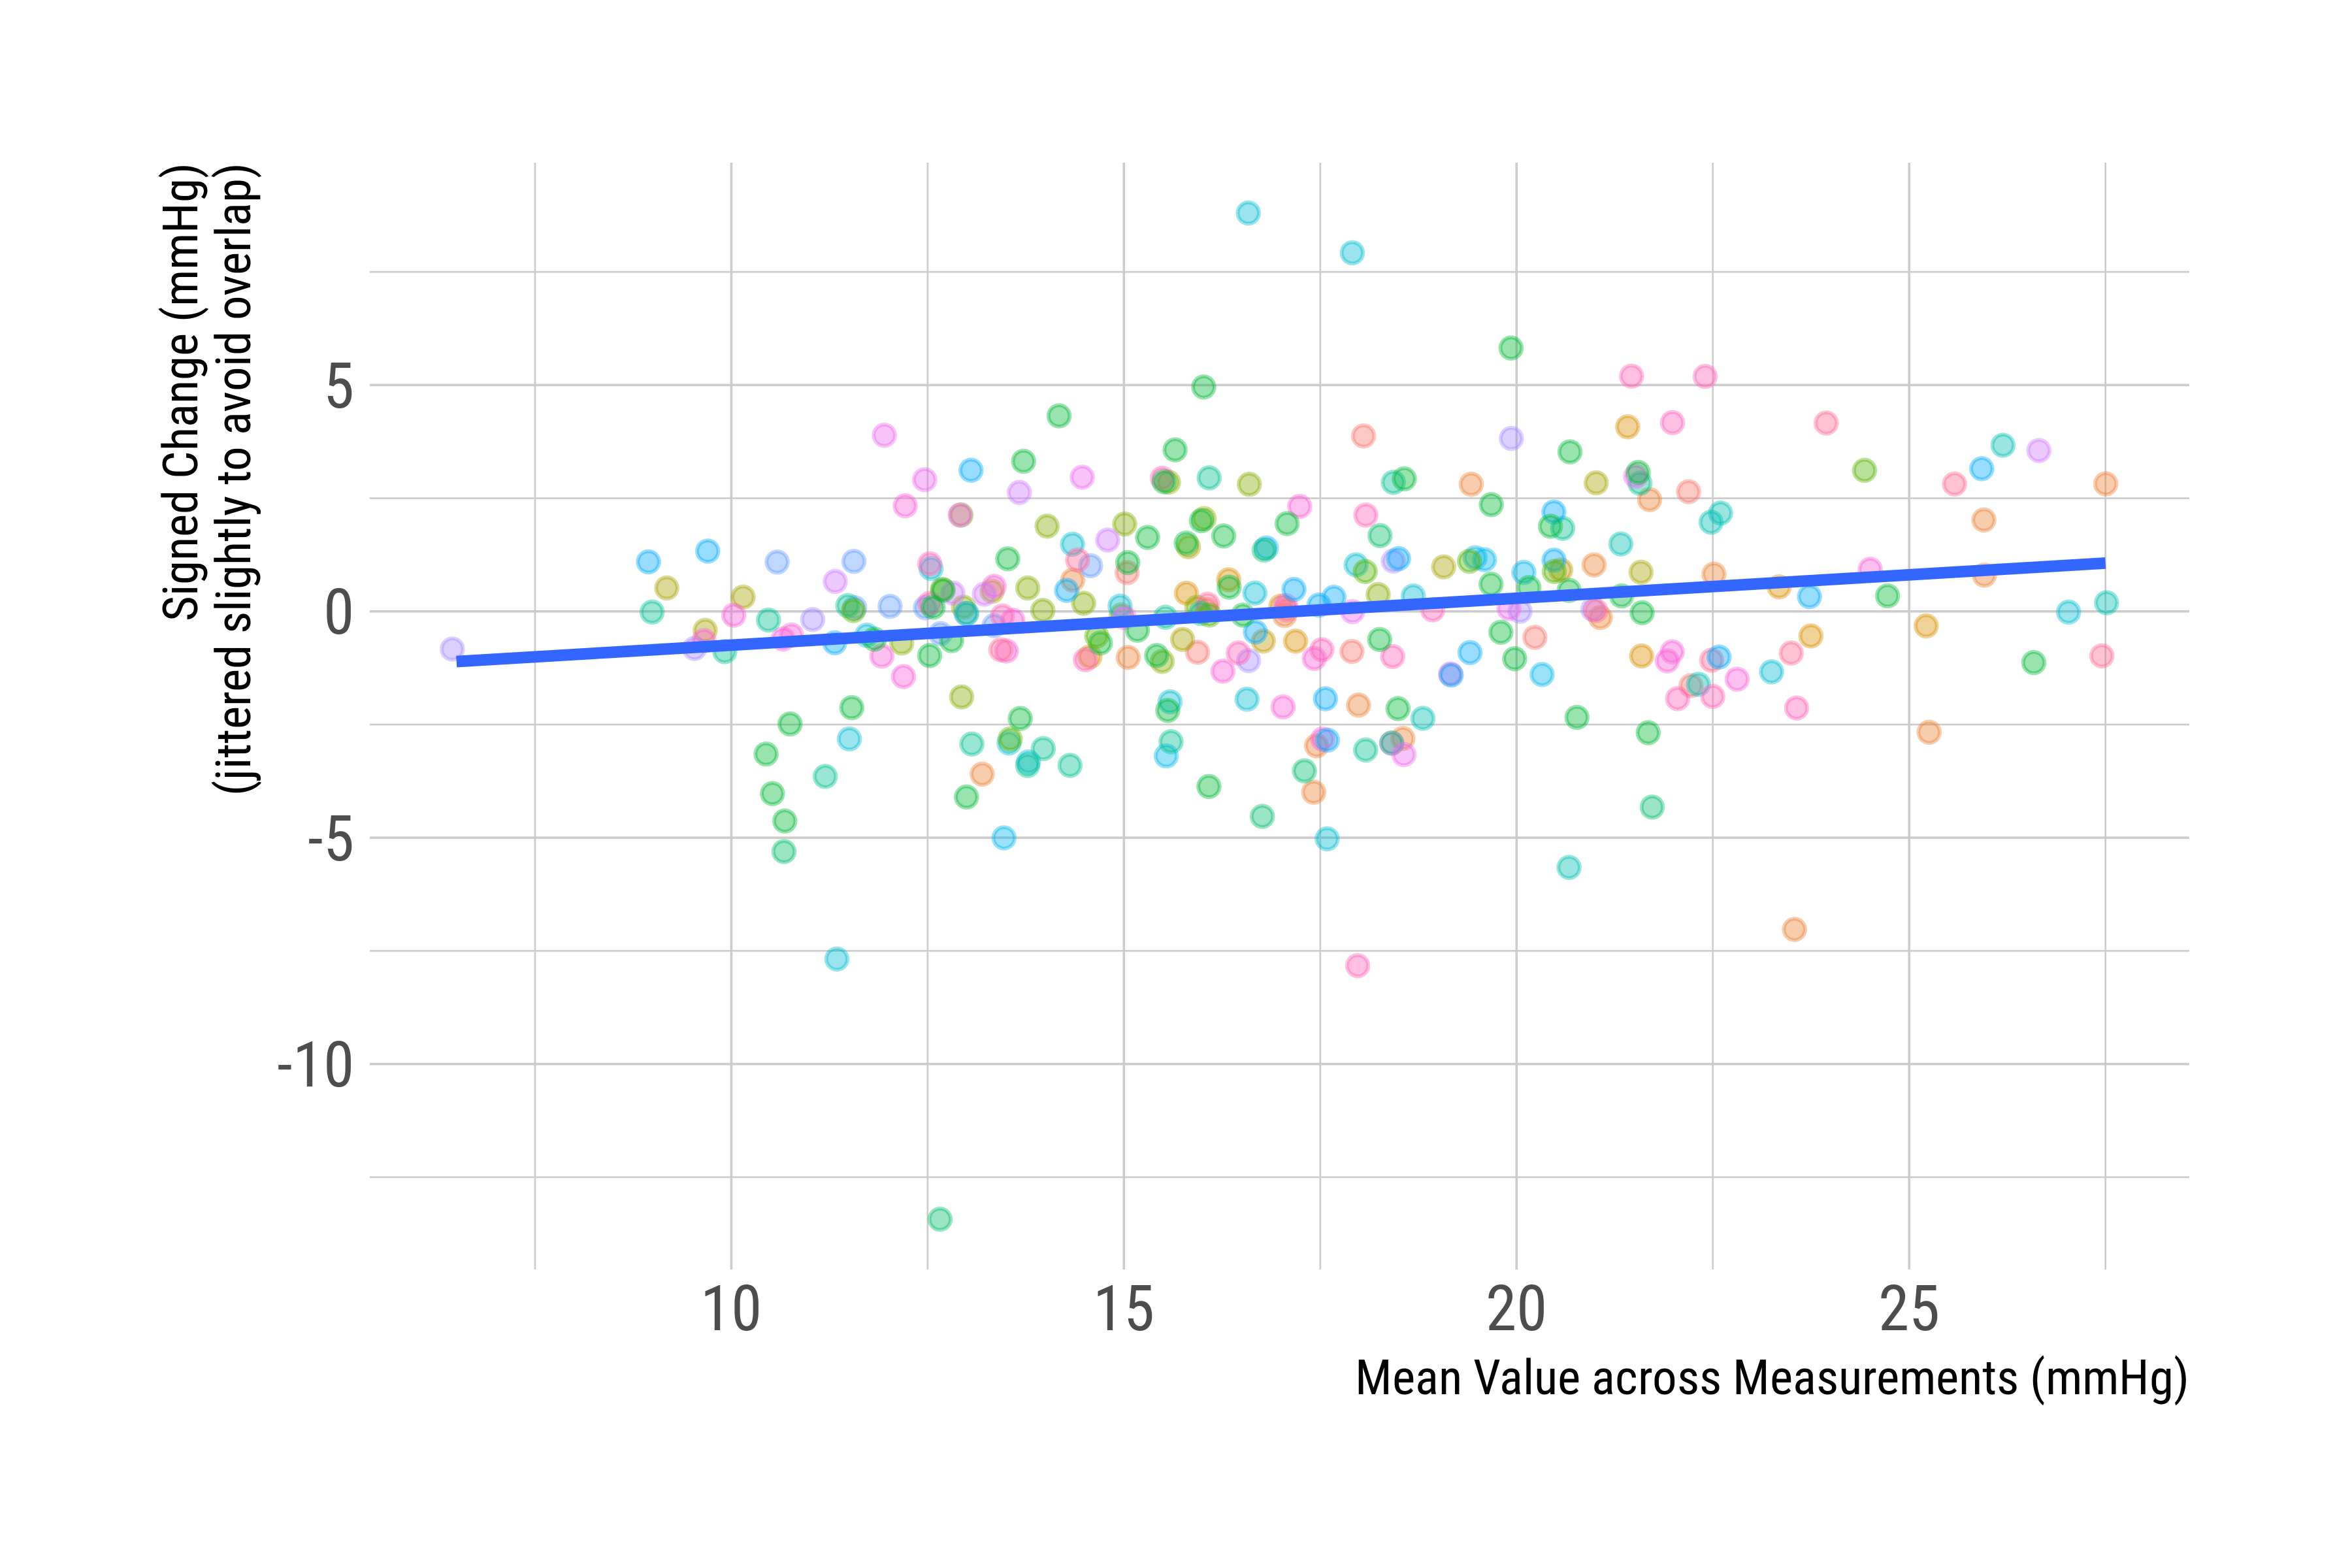
\includegraphics{figures/unnamed-chunk-49-1.png}

\hypertarget{figures-1}{%
\subsection{Figures}\label{figures-1}}

\begin{Shaded}
\begin{Highlighting}[]
\NormalTok{cowplot}\SpecialCharTok{::}\FunctionTok{plot\_grid}\NormalTok{(decomp\_plot, days\_plot,}
\NormalTok{                   perc\_alc\_plot, centre\_plot, }\AttributeTok{align =} \StringTok{"hv"}\NormalTok{, }
                   \AttributeTok{ncol =} \DecValTok{2}\NormalTok{, }\AttributeTok{labels =} \StringTok{"AUTO"}\NormalTok{)}
\end{Highlighting}
\end{Shaded}

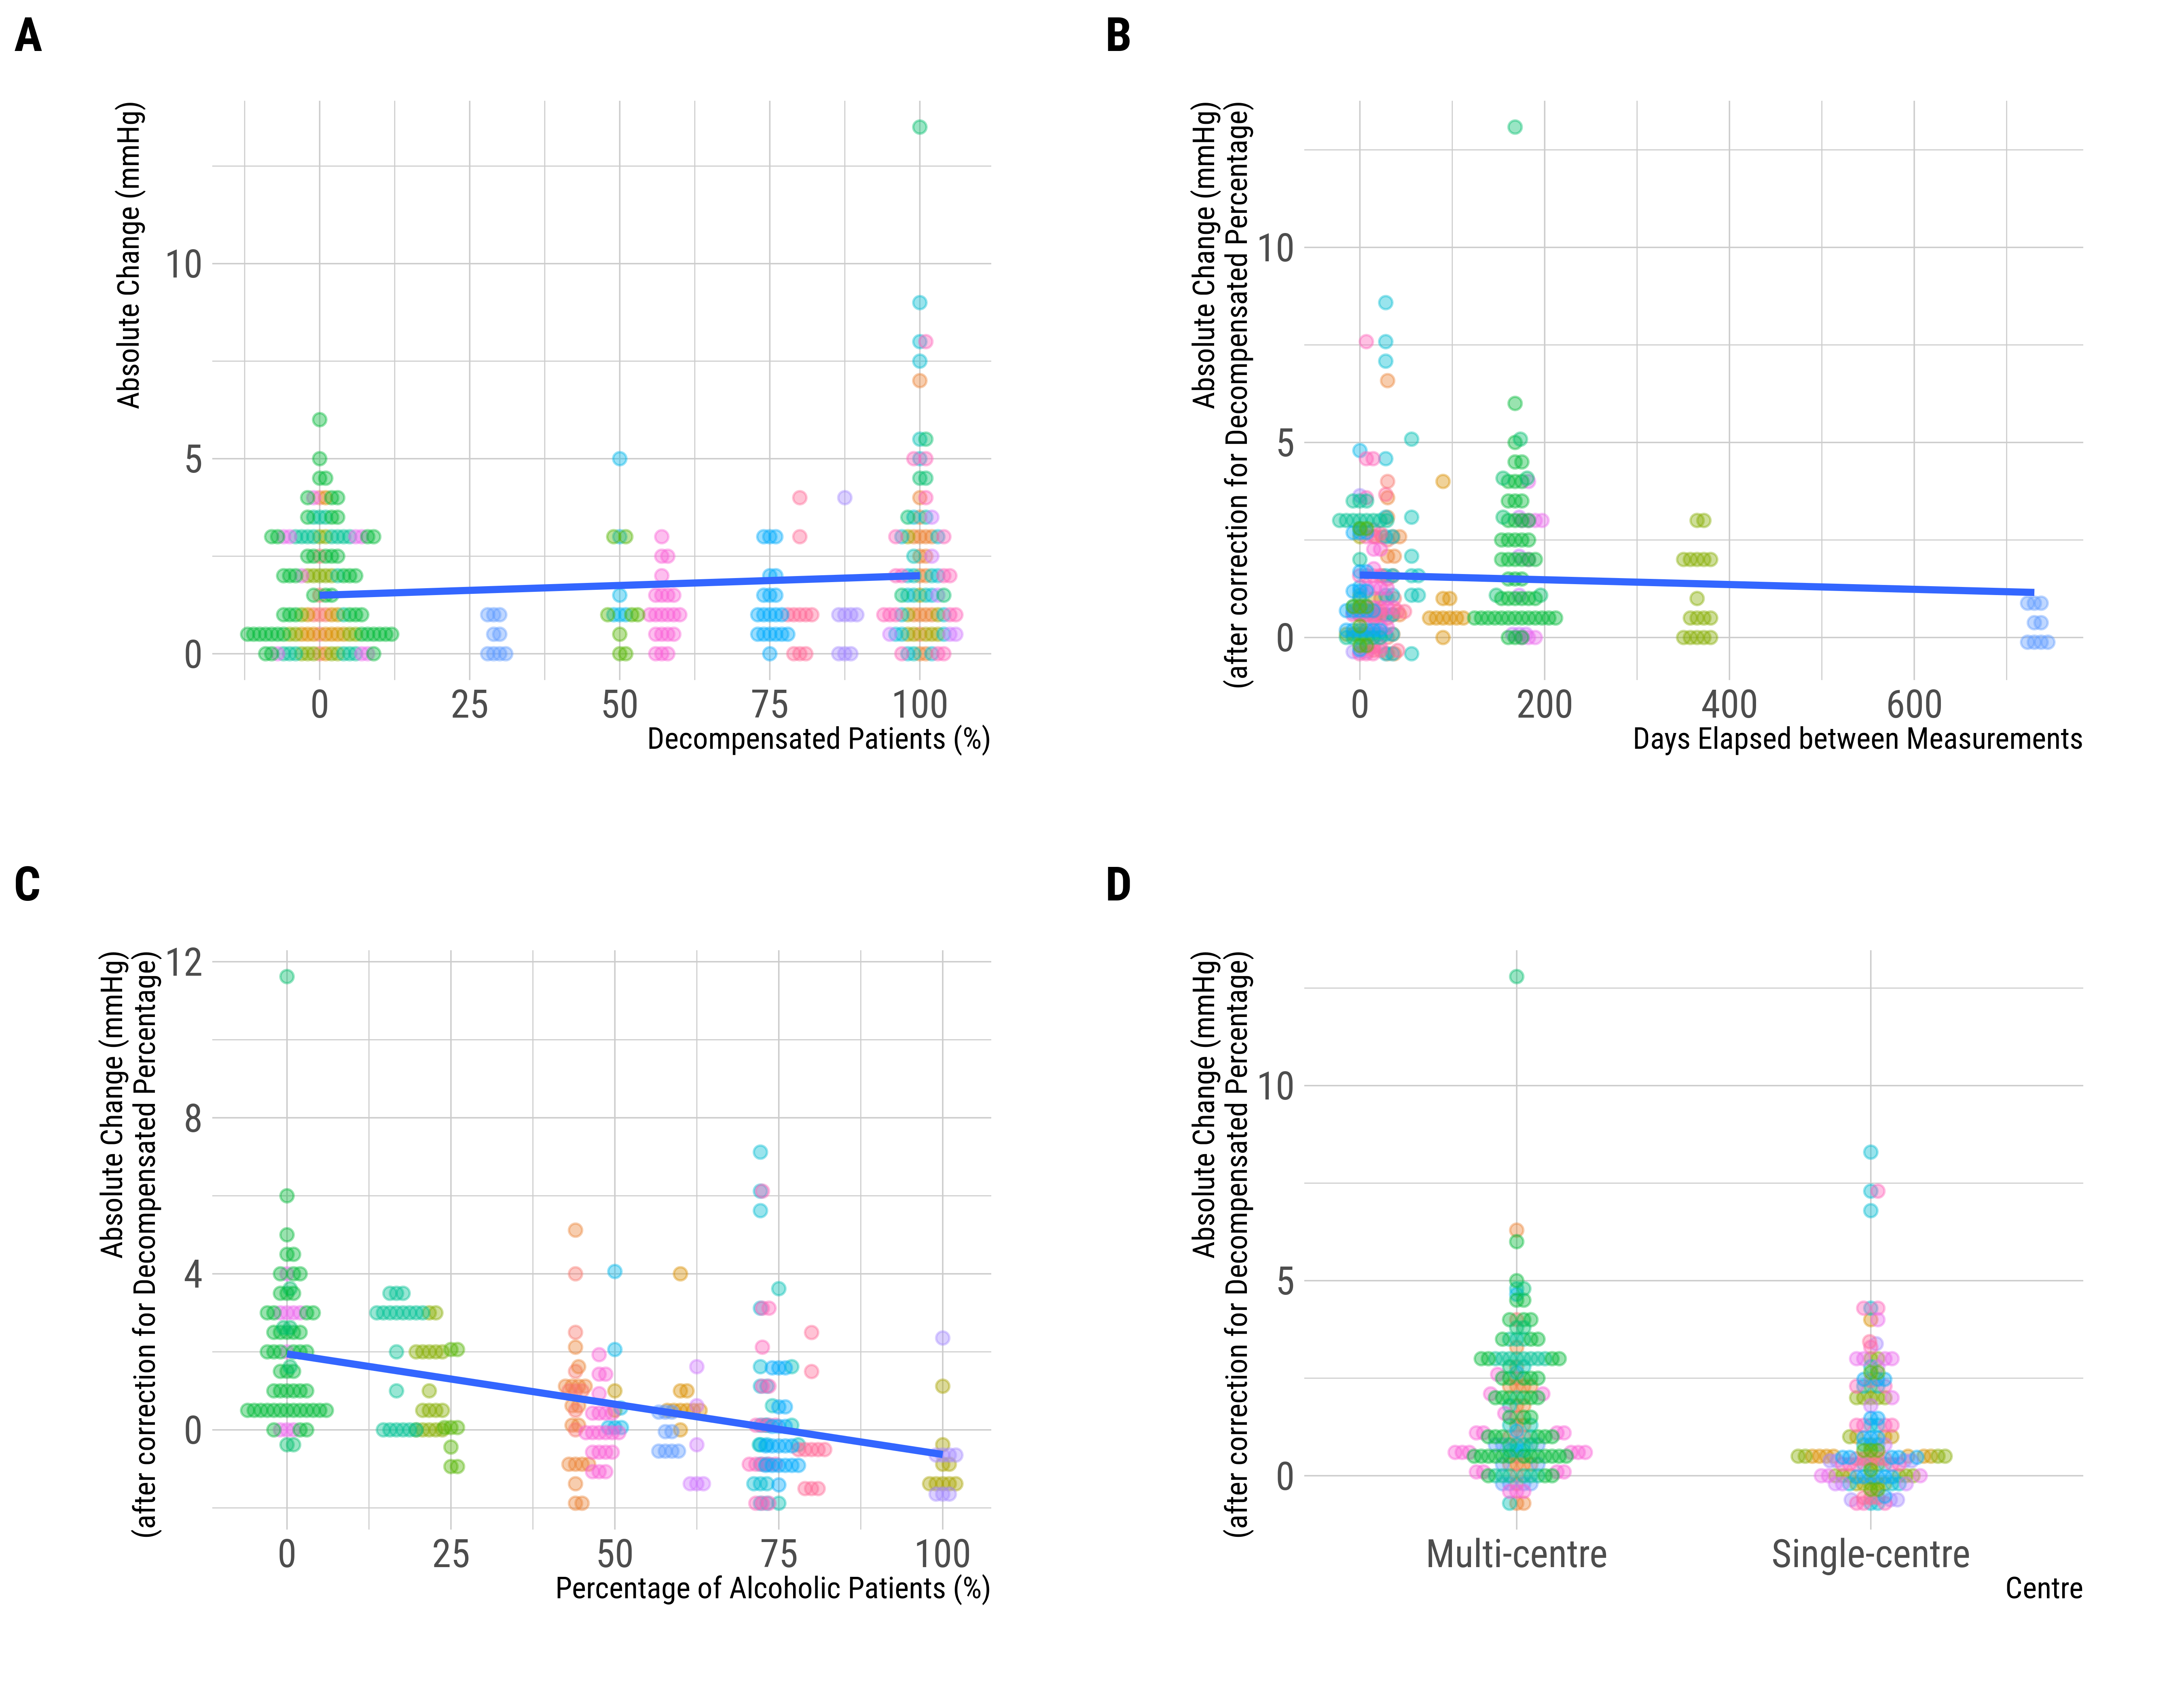
\includegraphics{figures/unnamed-chunk-50-1.png}

\begin{Shaded}
\begin{Highlighting}[]
\NormalTok{cowplot}\SpecialCharTok{::}\FunctionTok{plot\_grid}\NormalTok{(abs\_change\_distr, sign\_change\_distr,}
\NormalTok{                   meanv\_abs\_plot, meanv\_signed\_plot, }
                   \AttributeTok{align =} \StringTok{"hv"}\NormalTok{, }
                   \AttributeTok{ncol =} \DecValTok{2}\NormalTok{, }\AttributeTok{labels =} \StringTok{"AUTO"}\NormalTok{)}
\end{Highlighting}
\end{Shaded}

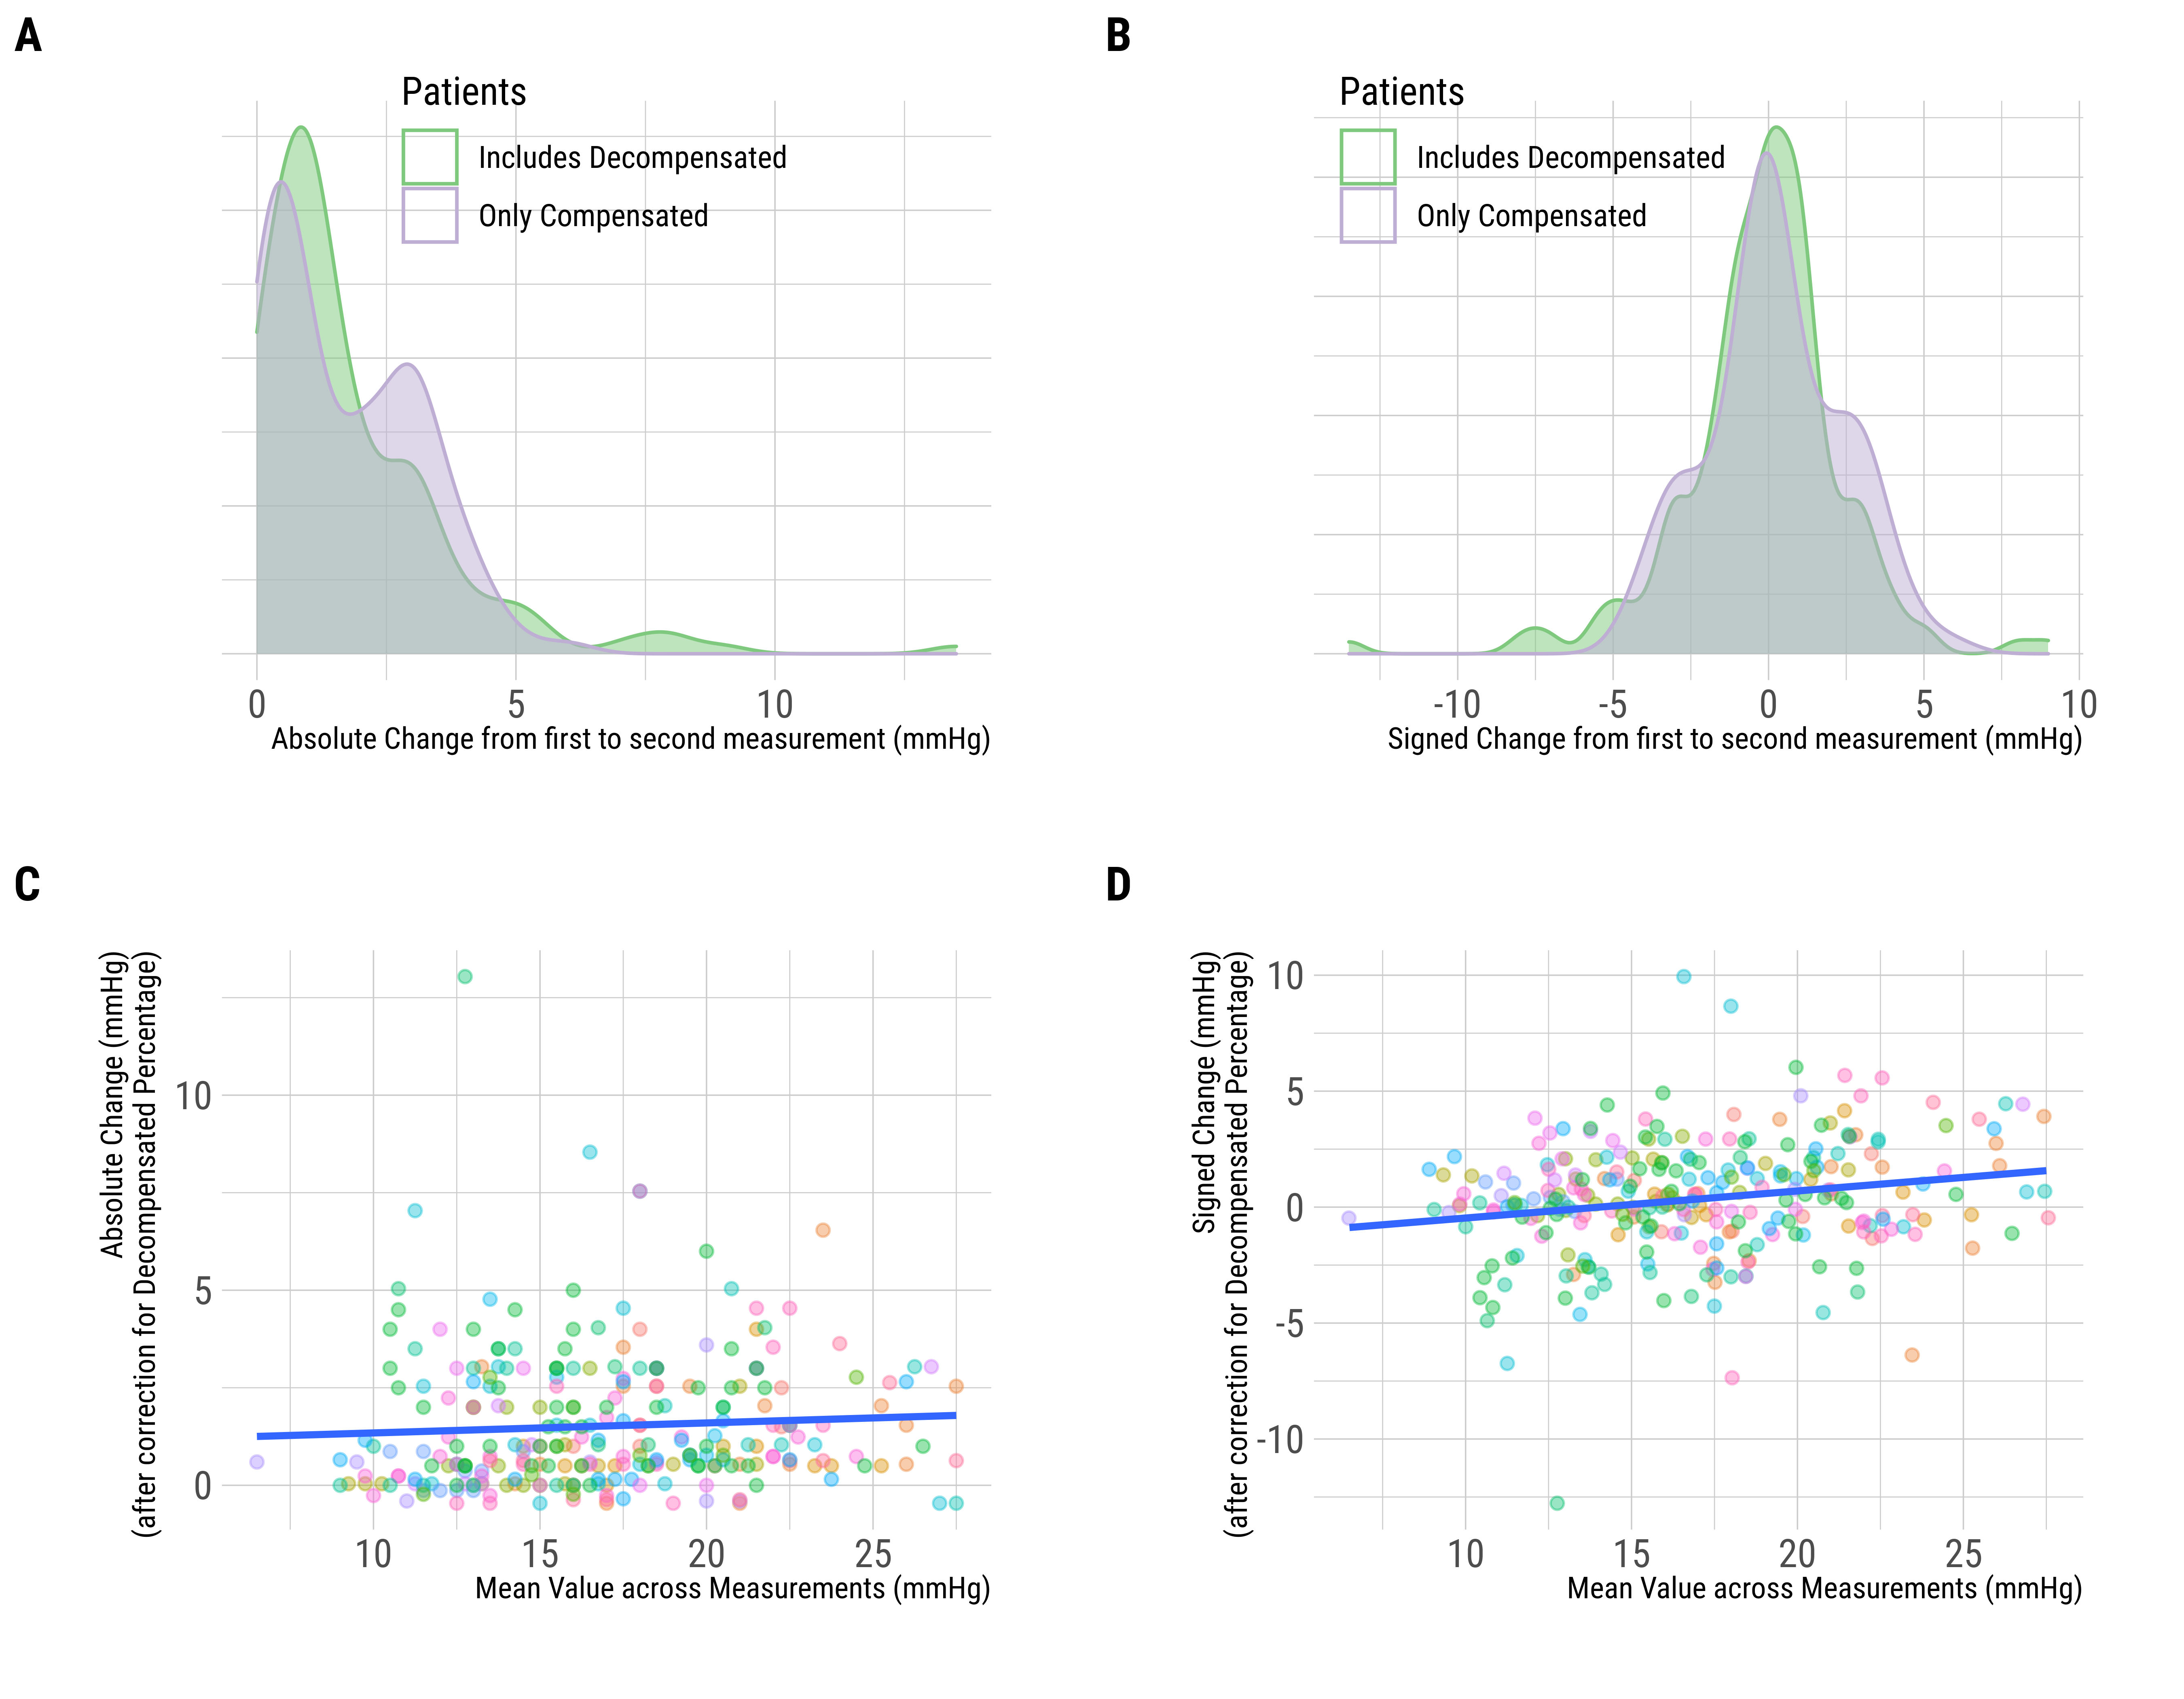
\includegraphics{figures/unnamed-chunk-51-1.png}

\hypertarget{power-analysis-for-a-difference}{%
\section{Power Analysis for a
difference}\label{power-analysis-for-a-difference}}

Now, the core thing we want to do here is to perform a power analysis
for examining within-individual effects.

One way of doing this is to use the \texttt{signvar\_sd} column of the
\texttt{tidytrt} object. This is the standard deviation of the signed
changes, and hence, if we assume a change after an intervention, this is
the SD we could imagine being true, and thus, the effect size, the
Cohen's Dz, is equal to difference / signvar\_sd. However, this method
makes an assumption that everyone changes by exactly the same amount:
the effect (before accounting for error) is completely uniform. This may
be the case, but this is the most optimistic scenario. We should be
taking into consideration the possibility of heterogeneous effects.

First, let's make a little plot to show what I mean by homogeneous and
heterogeneous effects.

\begin{Shaded}
\begin{Highlighting}[]
\FunctionTok{set.seed}\NormalTok{(}\DecValTok{1234}\NormalTok{)}

\NormalTok{trt\_all\_comp }\OtherTok{\textless{}{-}}\NormalTok{ trt\_all[}\DecValTok{2}\NormalTok{,]}

\NormalTok{wscv}\OtherTok{=}\NormalTok{trt\_all\_comp}\SpecialCharTok{$}\NormalTok{wscv}
\NormalTok{meanval}\OtherTok{=}\NormalTok{trt\_all\_comp}\SpecialCharTok{$}\NormalTok{mean}
\NormalTok{cv}\OtherTok{=}\NormalTok{trt\_all\_comp}\SpecialCharTok{$}\NormalTok{cv}
\NormalTok{icc}\OtherTok{=}\NormalTok{trt\_all\_comp}\SpecialCharTok{$}\NormalTok{icc}

\NormalTok{sd\_true }\OtherTok{\textless{}{-}} \FunctionTok{sqrt}\NormalTok{(icc }\SpecialCharTok{*}\NormalTok{ (cv }\SpecialCharTok{*}\NormalTok{ meanval)}\SpecialCharTok{\^{}}\DecValTok{2}\NormalTok{)}

\NormalTok{n }\OtherTok{\textless{}{-}} \DecValTok{20}
\NormalTok{delta }\OtherTok{\textless{}{-}} \DecValTok{2}

\CommentTok{\# Homogeneous}
\NormalTok{cv\_delta }\OtherTok{\textless{}{-}} \DecValTok{0}

\NormalTok{pre\_true }\OtherTok{\textless{}{-}} \FunctionTok{rnorm}\NormalTok{(n, meanval, sd\_true)}
\NormalTok{pre\_meas }\OtherTok{\textless{}{-}}\NormalTok{ pre\_true }\SpecialCharTok{+} \FunctionTok{rnorm}\NormalTok{(n, }\DecValTok{0}\NormalTok{, meanval}\SpecialCharTok{*}\NormalTok{wscv)}

\NormalTok{post\_true }\OtherTok{\textless{}{-}}\NormalTok{ pre\_true }\SpecialCharTok{{-}} \FunctionTok{rnorm}\NormalTok{(n, delta, cv\_delta}\SpecialCharTok{*}\NormalTok{delta)}
\NormalTok{post\_meas }\OtherTok{\textless{}{-}}\NormalTok{ post\_true }\SpecialCharTok{+} \FunctionTok{rnorm}\NormalTok{(n, }\DecValTok{0}\NormalTok{, meanval}\SpecialCharTok{*}\NormalTok{wscv)}

\NormalTok{hom\_true }\OtherTok{\textless{}{-}}\NormalTok{ tibble}\SpecialCharTok{::}\FunctionTok{tibble}\NormalTok{(}
  \AttributeTok{ID =} \FunctionTok{rep}\NormalTok{(}\DecValTok{1}\SpecialCharTok{:}\NormalTok{n, }\AttributeTok{times=}\DecValTok{2}\NormalTok{),}
  \AttributeTok{Outcome =} \FunctionTok{c}\NormalTok{(pre\_true, post\_true),}
  \AttributeTok{PrePost =} \FunctionTok{rep}\NormalTok{(}\FunctionTok{c}\NormalTok{(}\StringTok{"Pre"}\NormalTok{, }\StringTok{"Post"}\NormalTok{), }\AttributeTok{each=}\NormalTok{n),}
  \AttributeTok{Effects =} \StringTok{"Homogeneous Effects"}\NormalTok{,}
  \AttributeTok{MeasuredTrue =} \StringTok{"True Values"}
\NormalTok{)}

\NormalTok{hom\_measured }\OtherTok{\textless{}{-}}\NormalTok{ tibble}\SpecialCharTok{::}\FunctionTok{tibble}\NormalTok{(}
  \AttributeTok{ID =} \FunctionTok{rep}\NormalTok{(}\DecValTok{1}\SpecialCharTok{:}\NormalTok{n, }\AttributeTok{times=}\DecValTok{2}\NormalTok{),}
  \AttributeTok{Outcome =} \FunctionTok{c}\NormalTok{(pre\_meas, post\_meas),}
  \AttributeTok{PrePost =} \FunctionTok{rep}\NormalTok{(}\FunctionTok{c}\NormalTok{(}\StringTok{"Pre"}\NormalTok{, }\StringTok{"Post"}\NormalTok{), }\AttributeTok{each=}\NormalTok{n),}
  \AttributeTok{Effects =} \StringTok{"Homogeneous Effects"}\NormalTok{,}
  \AttributeTok{MeasuredTrue =} \StringTok{"Measured Values"}
\NormalTok{)}

\CommentTok{\# hom\_difference \textless{}{-} tibble::tibble(}
\CommentTok{\#   ID = rep(1:n, times=2),}
\CommentTok{\#   Outcome = c(post\_meas{-}pre\_),}
\CommentTok{\#   PrePost = rep(c("Pre", "Post"), each=n),}
\CommentTok{\#   Effects = "Homogeneous",}
\CommentTok{\#   MeasuredTrue = "Difference"}
\CommentTok{\# )}


\CommentTok{\# Heterogeneous}
\NormalTok{cv\_delta }\OtherTok{\textless{}{-}} \FloatTok{0.5}

\CommentTok{\#pre\_true \textless{}{-} rnorm(n, meanval, abs(cv*meanval)) \# Use same as above}
\CommentTok{\#pre\_meas \textless{}{-} pre\_true + rnorm(n, 0, abs(meanval*wscv))}

\NormalTok{post\_true }\OtherTok{\textless{}{-}}\NormalTok{ pre\_true }\SpecialCharTok{{-}} \FunctionTok{rnorm}\NormalTok{(n, delta, }\FunctionTok{abs}\NormalTok{(cv\_delta}\SpecialCharTok{*}\NormalTok{delta))}
\NormalTok{post\_meas }\OtherTok{\textless{}{-}}\NormalTok{ post\_true }\SpecialCharTok{+} \FunctionTok{rnorm}\NormalTok{(n, }\DecValTok{0}\NormalTok{, }\FunctionTok{abs}\NormalTok{(meanval}\SpecialCharTok{*}\NormalTok{wscv))}

\NormalTok{het\_true }\OtherTok{\textless{}{-}}\NormalTok{ tibble}\SpecialCharTok{::}\FunctionTok{tibble}\NormalTok{(}
  \AttributeTok{ID =} \FunctionTok{rep}\NormalTok{(}\DecValTok{1}\SpecialCharTok{:}\NormalTok{n, }\AttributeTok{times=}\DecValTok{2}\NormalTok{),}
  \AttributeTok{Outcome =} \FunctionTok{c}\NormalTok{(pre\_true, post\_true),}
  \AttributeTok{PrePost =} \FunctionTok{rep}\NormalTok{(}\FunctionTok{c}\NormalTok{(}\StringTok{"Pre"}\NormalTok{, }\StringTok{"Post"}\NormalTok{), }\AttributeTok{each=}\NormalTok{n),}
  \AttributeTok{Effects =} \StringTok{"Heterogeneous Effects"}\NormalTok{,}
  \AttributeTok{MeasuredTrue =} \StringTok{"True Values"}
\NormalTok{)}

\NormalTok{het\_measured }\OtherTok{\textless{}{-}}\NormalTok{ tibble}\SpecialCharTok{::}\FunctionTok{tibble}\NormalTok{(}
  \AttributeTok{ID =} \FunctionTok{rep}\NormalTok{(}\DecValTok{1}\SpecialCharTok{:}\NormalTok{n, }\AttributeTok{times=}\DecValTok{2}\NormalTok{),}
  \AttributeTok{Outcome =} \FunctionTok{c}\NormalTok{(pre\_meas, post\_meas),}
  \AttributeTok{PrePost =} \FunctionTok{rep}\NormalTok{(}\FunctionTok{c}\NormalTok{(}\StringTok{"Pre"}\NormalTok{, }\StringTok{"Post"}\NormalTok{), }\AttributeTok{each=}\NormalTok{n),}
  \AttributeTok{Effects =} \StringTok{"Heterogeneous Effects"}\NormalTok{,}
  \AttributeTok{MeasuredTrue =} \StringTok{"Measured Values"}
\NormalTok{)}

\CommentTok{\# Plot}
\NormalTok{effects }\OtherTok{\textless{}{-}} \FunctionTok{bind\_rows}\NormalTok{(hom\_true, hom\_measured, het\_true, het\_measured) }\SpecialCharTok{\%\textgreater{}\%} 
  \FunctionTok{mutate}\NormalTok{(}\AttributeTok{MeasuredTrue =} \FunctionTok{fct\_inorder}\NormalTok{(MeasuredTrue),}
         \AttributeTok{Effects =} \FunctionTok{fct\_inorder}\NormalTok{(Effects),}
         \AttributeTok{PrePost =} \FunctionTok{fct\_inorder}\NormalTok{(PrePost),}
         \AttributeTok{ID =} \FunctionTok{as.factor}\NormalTok{(ID))}

\FunctionTok{ggplot}\NormalTok{(effects, }\FunctionTok{aes}\NormalTok{(}\AttributeTok{x=}\NormalTok{PrePost, }\AttributeTok{y=}\NormalTok{Outcome, }\AttributeTok{colour=}\NormalTok{ID, }\AttributeTok{group=}\NormalTok{ID)) }\SpecialCharTok{+}
  \FunctionTok{geom\_point}\NormalTok{(}\AttributeTok{size=}\DecValTok{2}\NormalTok{) }\SpecialCharTok{+}
  \FunctionTok{geom\_line}\NormalTok{() }\SpecialCharTok{+}
  \FunctionTok{facet\_grid}\NormalTok{(Effects}\SpecialCharTok{\textasciitilde{}}\NormalTok{MeasuredTrue) }\SpecialCharTok{+}
  \FunctionTok{labs}\NormalTok{(}\AttributeTok{y=}\StringTok{"Outcome (mmHg)"}\NormalTok{,}
       \AttributeTok{colour=}\StringTok{"Values"}\NormalTok{,}
       \AttributeTok{x=}\ConstantTok{NULL}\NormalTok{,}
       \AttributeTok{title=}\StringTok{"Homogeneous and Heteregeneous Effects"}\NormalTok{,}
       \AttributeTok{subtitle=}\StringTok{"Homogeneous effects imply that the true underlying change is the same}\SpecialCharTok{\textbackslash{}n}\StringTok{in all individuals (hence parallel lines in the true values)"}\NormalTok{) }\SpecialCharTok{+}
  \FunctionTok{guides}\NormalTok{(}\AttributeTok{colour=}\ConstantTok{FALSE}\NormalTok{)}
\end{Highlighting}
\end{Shaded}

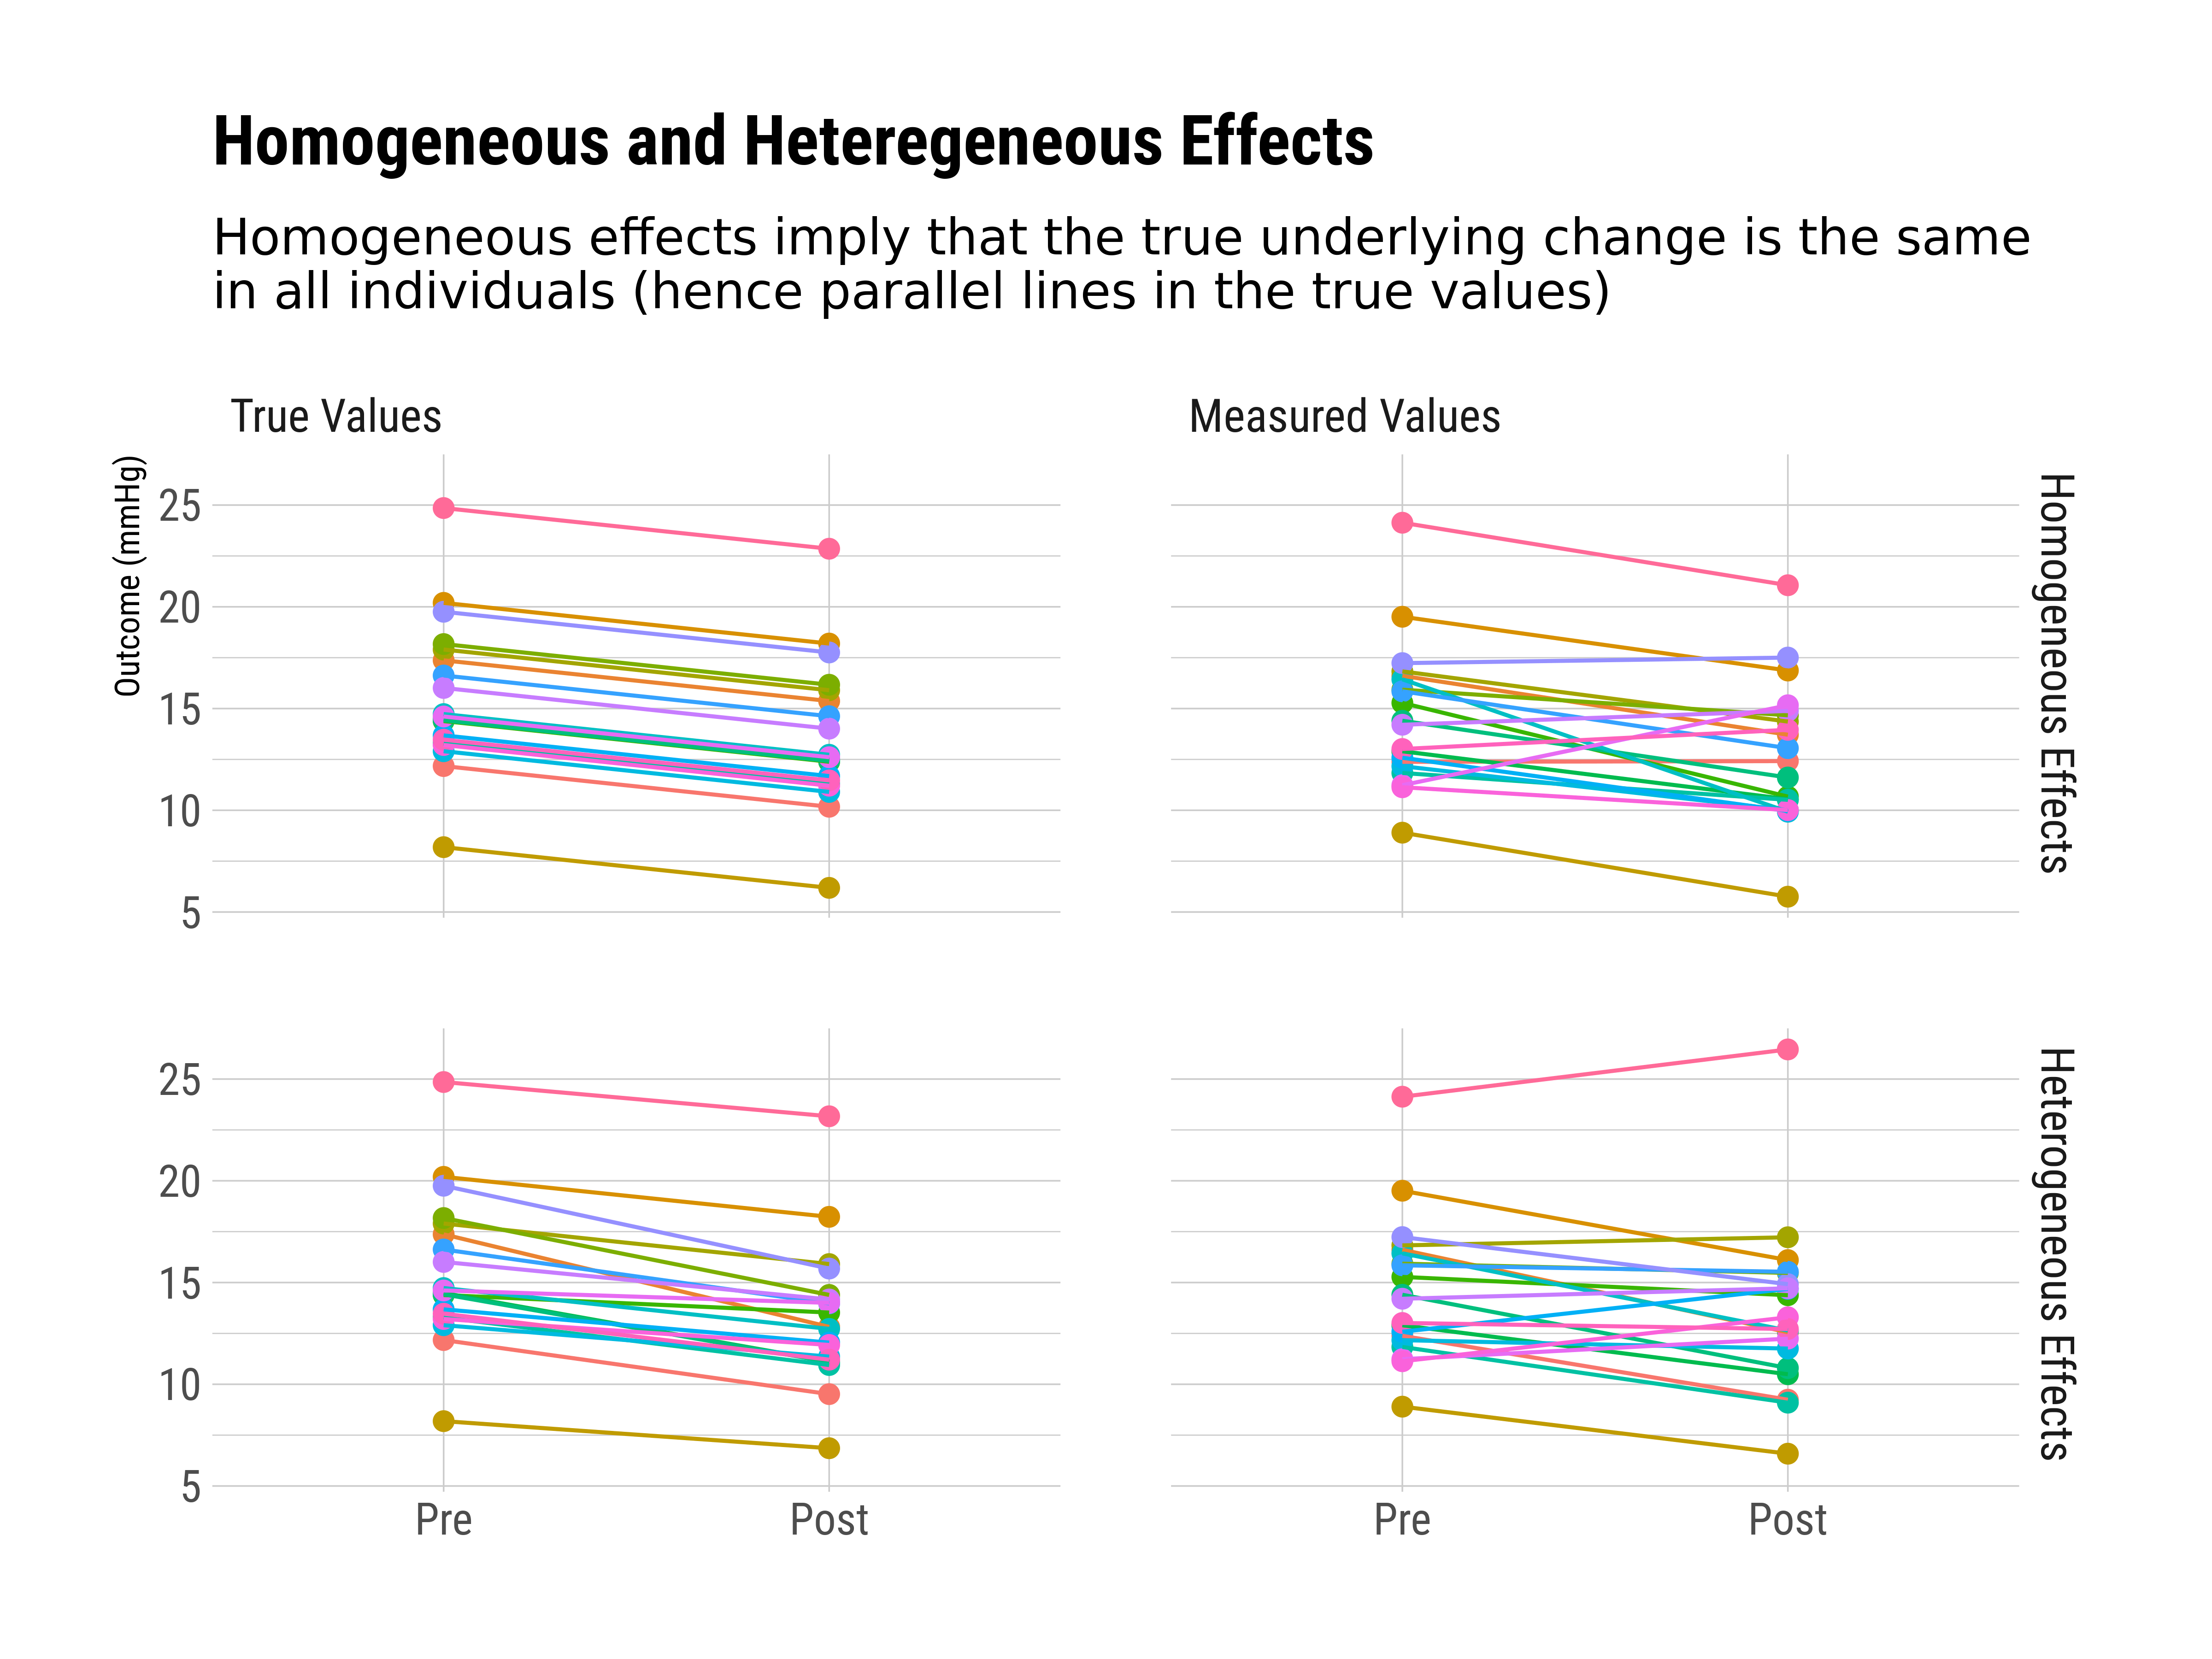
\includegraphics{figures/unnamed-chunk-52-1.png}

So, to summarise, we have underlying true values, and measured values
after accounting for measurement error. The change from before to after
the intervention can either be homogeneous (everyone has exactly the
same effect), or heterogeneous (effect sizes differ, and some even get
harmed by the intervention - about 2.5\% as I've chosen the SD of the
intervention effect as 50\% of the mean effect, so 0 effect is 2 SDs
away from the mean effect size, which is approximately 2.5\%). Then, the
measured values appear to show more people getting worse after
treatment, but this is just due to measurement error.

\begin{Shaded}
\begin{Highlighting}[]
\NormalTok{heterogen\_cv }\OtherTok{\textless{}{-}} \FloatTok{0.5}

\NormalTok{annotations }\OtherTok{\textless{}{-}} \FunctionTok{tibble}\NormalTok{(}
  \AttributeTok{x=}\FunctionTok{c}\NormalTok{(}\SpecialCharTok{{-}}\DecValTok{3}\NormalTok{, }\DecValTok{0}\NormalTok{),}
  \AttributeTok{text=}\FunctionTok{c}\NormalTok{(}\FunctionTok{paste0}\NormalTok{(}\FunctionTok{round}\NormalTok{(}\DecValTok{100}\SpecialCharTok{*}\FunctionTok{pnorm}\NormalTok{(}\DecValTok{1}\SpecialCharTok{/}\NormalTok{heterogen\_cv)), }\StringTok{"\% experience improvements"}\NormalTok{),}
         \FunctionTok{paste0}\NormalTok{(}\DecValTok{100}\SpecialCharTok{{-}}\FunctionTok{round}\NormalTok{(}\DecValTok{100}\SpecialCharTok{*}\FunctionTok{pnorm}\NormalTok{(}\DecValTok{1}\SpecialCharTok{/}\NormalTok{heterogen\_cv)), }\StringTok{"\% experience worsening"}\NormalTok{)),}
  \AttributeTok{colour =} \FunctionTok{c}\NormalTok{(}\StringTok{"\#61b096"}\NormalTok{, }\StringTok{"\#bd7969"}\NormalTok{)}
\NormalTok{)}

\NormalTok{heterogen\_effects }\OtherTok{\textless{}{-}} \FunctionTok{tibble}\NormalTok{(}\AttributeTok{Effect=}\FunctionTok{c}\NormalTok{(}\SpecialCharTok{{-}}\DecValTok{3}\NormalTok{, }\DecValTok{1}\NormalTok{)) }

\FunctionTok{ggplot}\NormalTok{(heterogen\_effects, }\FunctionTok{aes}\NormalTok{(}\AttributeTok{x=}\NormalTok{Effect)) }\SpecialCharTok{+}
  \FunctionTok{geom\_area}\NormalTok{(}\AttributeTok{stat=}\StringTok{"function"}\NormalTok{, }\AttributeTok{fun =}\NormalTok{ dnorm, }\AttributeTok{fill=}\StringTok{"\#61b096"}\NormalTok{, }\AttributeTok{xlim=}\FunctionTok{c}\NormalTok{(}\SpecialCharTok{{-}}\DecValTok{3}\NormalTok{, }\DecValTok{0}\NormalTok{),}
            \AttributeTok{args =} \FunctionTok{list}\NormalTok{(}\AttributeTok{mean =} \SpecialCharTok{{-}}\DecValTok{1}\NormalTok{, }\AttributeTok{sd=}\NormalTok{heterogen\_cv), }\AttributeTok{alpha=}\FloatTok{0.7}\NormalTok{) }\SpecialCharTok{+}
  \FunctionTok{geom\_area}\NormalTok{(}\AttributeTok{stat=}\StringTok{"function"}\NormalTok{, }\AttributeTok{fun =}\NormalTok{ dnorm, }\AttributeTok{fill=}\StringTok{"\#bd7969"}\NormalTok{, }\AttributeTok{xlim=}\FunctionTok{c}\NormalTok{(}\DecValTok{0}\NormalTok{, }\DecValTok{1}\NormalTok{),}
            \AttributeTok{args =} \FunctionTok{list}\NormalTok{(}\AttributeTok{mean =} \SpecialCharTok{{-}}\DecValTok{1}\NormalTok{, }\AttributeTok{sd=}\NormalTok{heterogen\_cv), }\AttributeTok{alpha=}\FloatTok{0.7}\NormalTok{) }\SpecialCharTok{+}
  \FunctionTok{annotate}\NormalTok{(}\StringTok{"text"}\NormalTok{, }\AttributeTok{x=}\SpecialCharTok{{-}}\FloatTok{2.5}\NormalTok{, }\AttributeTok{y=}\FloatTok{0.7}\NormalTok{, }
           \AttributeTok{label=}\FunctionTok{paste0}\NormalTok{(}\FunctionTok{round}\NormalTok{(}\DecValTok{100}\SpecialCharTok{*}\FunctionTok{pnorm}\NormalTok{(}\DecValTok{1}\SpecialCharTok{/}\NormalTok{heterogen\_cv), }\DecValTok{1}\NormalTok{), }
                        \StringTok{"\% experience}\SpecialCharTok{\textbackslash{}n}\StringTok{improvements"}\NormalTok{),}
           \AttributeTok{colour =} \StringTok{"\#61b096"}\NormalTok{, }\AttributeTok{hjust=}\FloatTok{0.5}\NormalTok{) }\SpecialCharTok{+}
  \FunctionTok{annotate}\NormalTok{(}\StringTok{"text"}\NormalTok{, }\AttributeTok{x=}\FloatTok{0.5}\NormalTok{, }\AttributeTok{y=}\FloatTok{0.7}\NormalTok{, }
           \AttributeTok{label=}\FunctionTok{paste0}\NormalTok{(}\DecValTok{100}\SpecialCharTok{{-}}\FunctionTok{round}\NormalTok{(}\DecValTok{100}\SpecialCharTok{*}\FunctionTok{pnorm}\NormalTok{(}\DecValTok{1}\SpecialCharTok{/}\NormalTok{heterogen\_cv), }\DecValTok{1}\NormalTok{), }
                        \StringTok{"\% experience}\SpecialCharTok{\textbackslash{}n}\StringTok{worsening"}\NormalTok{),}
           \AttributeTok{colour =} \StringTok{"\#bd7969"}\NormalTok{, }\AttributeTok{hjust=}\FloatTok{0.5}\NormalTok{) }\SpecialCharTok{+}
  \FunctionTok{annotate}\NormalTok{(}\StringTok{"text"}\NormalTok{, }\AttributeTok{x=}\SpecialCharTok{{-}}\FloatTok{0.8}\NormalTok{, }\AttributeTok{y=}\FloatTok{0.2}\NormalTok{, }
           \AttributeTok{label=}\StringTok{"Mean}\SpecialCharTok{\textbackslash{}n}\StringTok{effect"}\NormalTok{,}\AttributeTok{hjust=}\FloatTok{0.5}\NormalTok{) }\SpecialCharTok{+}
  \FunctionTok{theme}\NormalTok{(}\AttributeTok{axis.title.y=}\FunctionTok{element\_blank}\NormalTok{(),}
        \AttributeTok{axis.text.y=}\FunctionTok{element\_blank}\NormalTok{(),}
        \AttributeTok{axis.ticks.y=}\FunctionTok{element\_blank}\NormalTok{()) }\SpecialCharTok{+}
  \FunctionTok{geom\_vline}\NormalTok{(}\AttributeTok{xintercept =} \SpecialCharTok{{-}}\DecValTok{1}\NormalTok{) }\SpecialCharTok{+}
  \FunctionTok{labs}\NormalTok{(}\AttributeTok{title=}\StringTok{"Heterogeneous Effects"}\NormalTok{,}
       \AttributeTok{subtitle=}\FunctionTok{paste0}\NormalTok{(}\StringTok{"Using a 50\% CV for effect heterogeneity implies that some "}\NormalTok{,}
                       \StringTok{"participants}\SpecialCharTok{\textbackslash{}n}\StringTok{may benefit more and others may even have "}\NormalTok{,}
                       \StringTok{"worsening."}\NormalTok{))}
\end{Highlighting}
\end{Shaded}

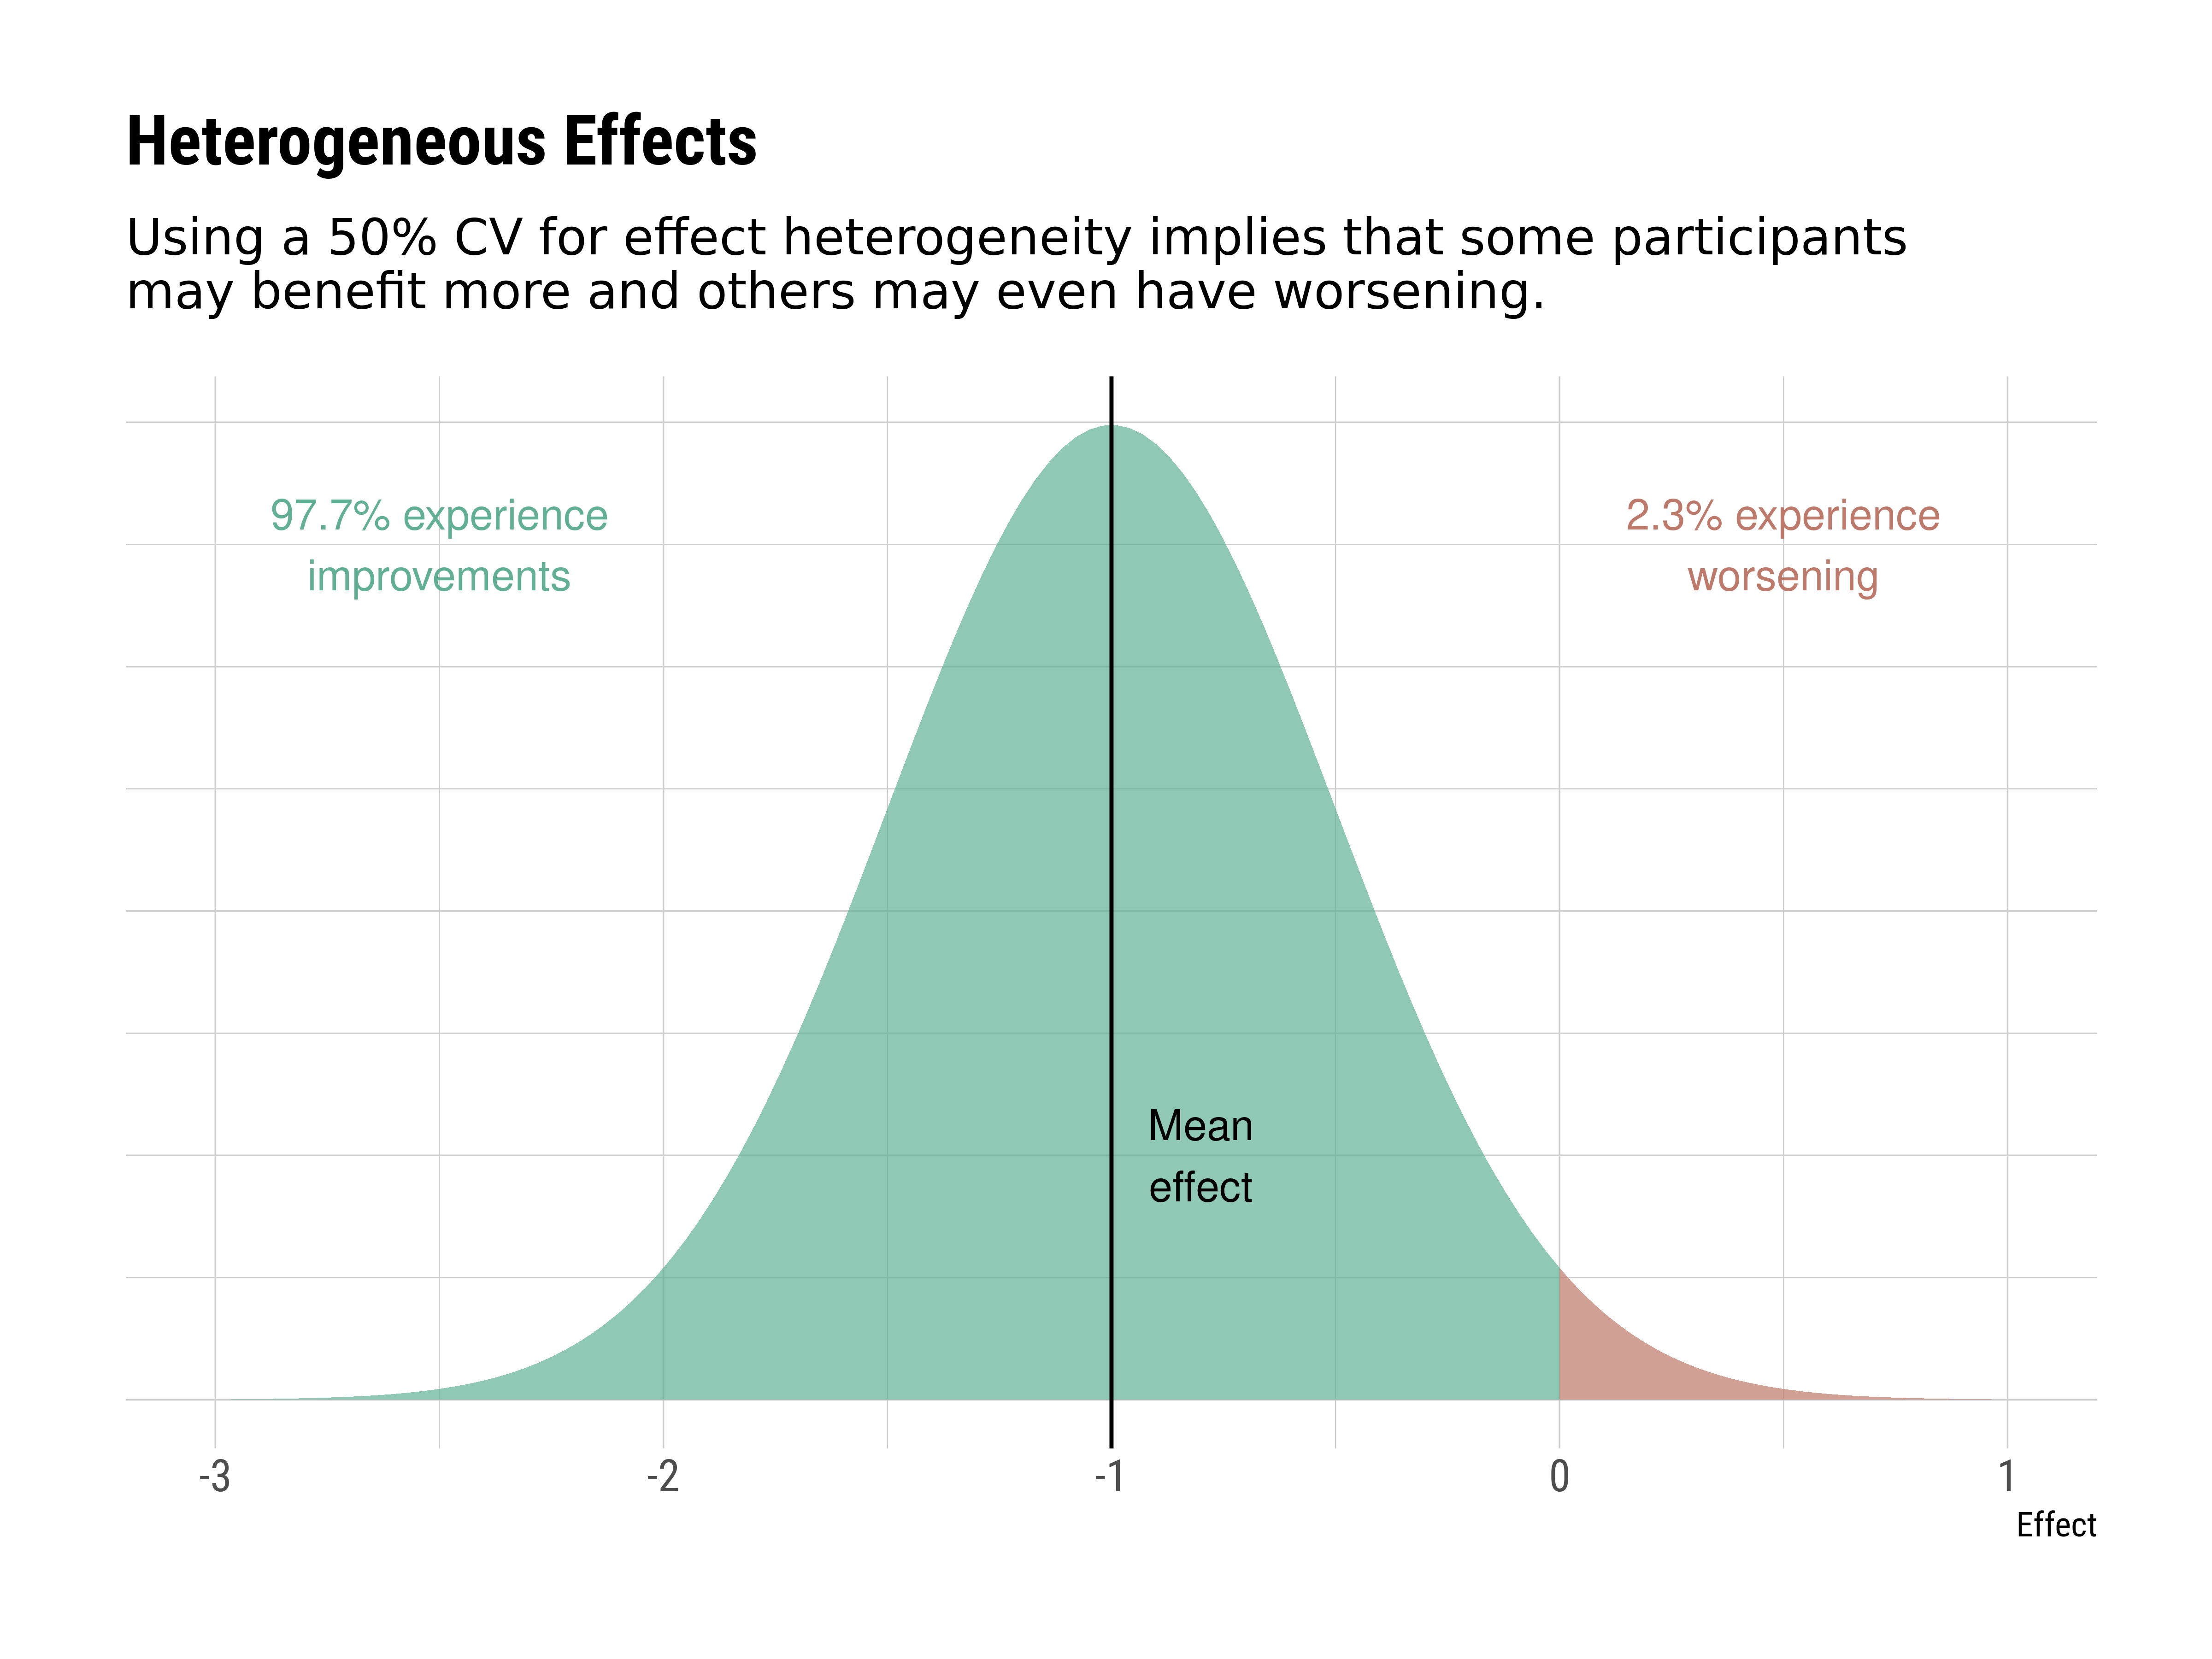
\includegraphics{figures/unnamed-chunk-53-1.png}

This would imply that for all different sizes of effect, that only 2.3\%
experience a true worsening. However, when we measure the values, there
are also several individuals who will exhibit an apparent worsening
(increases from first to second measurement), when their true underlying
values exhibited improvements. Let's calculate what fraction of
individuals this would be.

\hypertarget{true-and-apparent-changes}{%
\subsection{True and Apparent Changes}\label{true-and-apparent-changes}}

Here, we can also observe the percentage of individuals who show
apparent 10\% and 20\% changes from baseline.

\begin{Shaded}
\begin{Highlighting}[]
\NormalTok{apparent\_effects }\OtherTok{\textless{}{-}} \ControlFlowTok{function}\NormalTok{(n, delta, cv\_delta, }\AttributeTok{wscv=}\NormalTok{trt\_all}\SpecialCharTok{$}\NormalTok{wscv, }
                     \AttributeTok{mean=}\NormalTok{trt\_all}\SpecialCharTok{$}\NormalTok{mean, }\AttributeTok{cv=}\NormalTok{trt\_all}\SpecialCharTok{$}\NormalTok{cv, }\AttributeTok{icc=}\NormalTok{trt\_all}\SpecialCharTok{$}\NormalTok{icc, }
\NormalTok{                     decomp) \{}
  
\NormalTok{  wscv }\OtherTok{\textless{}{-}}\NormalTok{ wscv[decomp]}
\NormalTok{  mean }\OtherTok{\textless{}{-}}\NormalTok{ mean[decomp]}
\NormalTok{  cv   }\OtherTok{\textless{}{-}}\NormalTok{ cv[decomp]}
  
\NormalTok{  var }\OtherTok{\textless{}{-}}\NormalTok{ (cv}\SpecialCharTok{*}\NormalTok{mean)}\SpecialCharTok{\^{}}\DecValTok{2}
\NormalTok{  sd\_true }\OtherTok{\textless{}{-}} \FunctionTok{sqrt}\NormalTok{(var }\SpecialCharTok{*}\NormalTok{ icc)}
  
  
\NormalTok{  pre\_true }\OtherTok{\textless{}{-}} \FunctionTok{rnorm}\NormalTok{(n, mean, sd\_true)}
  
\NormalTok{  pre\_meas }\OtherTok{\textless{}{-}}\NormalTok{ pre\_true }\SpecialCharTok{+} \FunctionTok{rnorm}\NormalTok{(n, }\DecValTok{0}\NormalTok{, mean}\SpecialCharTok{*}\NormalTok{wscv)}
  
\NormalTok{  post\_true }\OtherTok{\textless{}{-}}\NormalTok{ pre\_true }\SpecialCharTok{{-}} \FunctionTok{rnorm}\NormalTok{(n, delta, cv\_delta}\SpecialCharTok{*}\NormalTok{delta)}
  
\NormalTok{  post\_meas }\OtherTok{\textless{}{-}}\NormalTok{ post\_true }\SpecialCharTok{+} \FunctionTok{rnorm}\NormalTok{(n, }\DecValTok{0}\NormalTok{, mean}\SpecialCharTok{*}\NormalTok{wscv)}
  
\NormalTok{  measured }\OtherTok{\textless{}{-}}\NormalTok{ tibble}\SpecialCharTok{::}\FunctionTok{tibble}\NormalTok{(}
    \AttributeTok{ID =} \FunctionTok{rep}\NormalTok{(}\DecValTok{1}\SpecialCharTok{:}\NormalTok{n, }\AttributeTok{times=}\DecValTok{2}\NormalTok{),}
    \AttributeTok{Outcome =} \FunctionTok{c}\NormalTok{(pre\_meas, post\_meas),}
    \AttributeTok{PrePost =} \FunctionTok{rep}\NormalTok{(}\FunctionTok{c}\NormalTok{(}\StringTok{"Pre"}\NormalTok{, }\StringTok{"Post"}\NormalTok{), }\AttributeTok{each=}\NormalTok{n)}
\NormalTok{  ) }\SpecialCharTok{\%\textgreater{}\%} 
    \FunctionTok{spread}\NormalTok{(PrePost, Outcome)}
  
\NormalTok{  true }\OtherTok{\textless{}{-}}\NormalTok{ tibble}\SpecialCharTok{::}\FunctionTok{tibble}\NormalTok{(}
    \AttributeTok{ID =} \FunctionTok{rep}\NormalTok{(}\DecValTok{1}\SpecialCharTok{:}\NormalTok{n, }\AttributeTok{times=}\DecValTok{2}\NormalTok{),}
    \AttributeTok{Outcome =} \FunctionTok{c}\NormalTok{(pre\_true, post\_true),}
    \AttributeTok{PrePost =} \FunctionTok{rep}\NormalTok{(}\FunctionTok{c}\NormalTok{(}\StringTok{"Pre"}\NormalTok{, }\StringTok{"Post"}\NormalTok{), }\AttributeTok{each=}\NormalTok{n)}
\NormalTok{  ) }\SpecialCharTok{\%\textgreater{}\%} 
    \FunctionTok{spread}\NormalTok{(PrePost, Outcome)}
  
\NormalTok{  out }\OtherTok{\textless{}{-}} \FunctionTok{list}\NormalTok{()}
  
\NormalTok{  out}\SpecialCharTok{$}\NormalTok{apparent\_worse }\OtherTok{\textless{}{-}} \FunctionTok{round}\NormalTok{(}\DecValTok{100}\SpecialCharTok{*}\FunctionTok{with}\NormalTok{(measured, }\FunctionTok{mean}\NormalTok{(Post }\SpecialCharTok{\textgreater{}}\NormalTok{ Pre)),}\DecValTok{1}\NormalTok{)}
\NormalTok{  out}\SpecialCharTok{$}\NormalTok{apparent\_10    }\OtherTok{\textless{}{-}} \FunctionTok{round}\NormalTok{(}\DecValTok{100}\SpecialCharTok{*}\FunctionTok{with}\NormalTok{(measured, }\FunctionTok{mean}\NormalTok{((Pre}\SpecialCharTok{{-}}\NormalTok{Post)}\SpecialCharTok{/}\NormalTok{Pre }\SpecialCharTok{\textgreater{}} \FloatTok{0.1}\NormalTok{)),}\DecValTok{1}\NormalTok{)}
\NormalTok{  out}\SpecialCharTok{$}\NormalTok{apparent\_20    }\OtherTok{\textless{}{-}} \FunctionTok{round}\NormalTok{(}\DecValTok{100}\SpecialCharTok{*}\FunctionTok{with}\NormalTok{(measured, }\FunctionTok{mean}\NormalTok{((Pre}\SpecialCharTok{{-}}\NormalTok{Post)}\SpecialCharTok{/}\NormalTok{Pre }\SpecialCharTok{\textgreater{}} \FloatTok{0.2}\NormalTok{)),}\DecValTok{1}\NormalTok{)}
\NormalTok{  out}\SpecialCharTok{$}\NormalTok{true\_worse     }\OtherTok{\textless{}{-}} \FunctionTok{round}\NormalTok{(}\DecValTok{100}\SpecialCharTok{*}\FunctionTok{with}\NormalTok{(true, }\FunctionTok{mean}\NormalTok{(Post }\SpecialCharTok{\textgreater{}}\NormalTok{ Pre)),}\DecValTok{1}\NormalTok{)}
\NormalTok{  out}\SpecialCharTok{$}\NormalTok{true\_10        }\OtherTok{\textless{}{-}} \FunctionTok{round}\NormalTok{(}\DecValTok{100}\SpecialCharTok{*}\FunctionTok{with}\NormalTok{(true, }\FunctionTok{mean}\NormalTok{((Pre}\SpecialCharTok{{-}}\NormalTok{Post)}\SpecialCharTok{/}\NormalTok{Pre }\SpecialCharTok{\textgreater{}} \FloatTok{0.1}\NormalTok{)),}\DecValTok{1}\NormalTok{)}
\NormalTok{  out}\SpecialCharTok{$}\NormalTok{true\_20        }\OtherTok{\textless{}{-}} \FunctionTok{round}\NormalTok{(}\DecValTok{100}\SpecialCharTok{*}\FunctionTok{with}\NormalTok{(true, }\FunctionTok{mean}\NormalTok{((Pre}\SpecialCharTok{{-}}\NormalTok{Post)}\SpecialCharTok{/}\NormalTok{Pre }\SpecialCharTok{\textgreater{}} \FloatTok{0.2}\NormalTok{)),}\DecValTok{1}\NormalTok{)}
  
  \FunctionTok{return}\NormalTok{(out)}

\NormalTok{\}}

\ControlFlowTok{if}\NormalTok{(}\SpecialCharTok{!}\FunctionTok{file.exists}\NormalTok{(}\StringTok{"../DerivedData/percdifs.rds"}\NormalTok{) }\SpecialCharTok{||}\NormalTok{ overwrite) \{}

\NormalTok{measured\_percs }\OtherTok{\textless{}{-}}\NormalTok{ tidyr}\SpecialCharTok{::}\FunctionTok{crossing}\NormalTok{(}
  \AttributeTok{delta =} \FunctionTok{seq}\NormalTok{(}\DecValTok{0}\NormalTok{, }\DecValTok{3}\NormalTok{, }\AttributeTok{by=}\FloatTok{0.5}\NormalTok{),}
  \AttributeTok{cv\_delta =} \FunctionTok{c}\NormalTok{(}\DecValTok{0}\NormalTok{, }\FloatTok{0.5}\NormalTok{),}
  \AttributeTok{decomp=}\FunctionTok{c}\NormalTok{(}\DecValTok{1}\NormalTok{,}\DecValTok{2}\NormalTok{)}
\NormalTok{) }\SpecialCharTok{\%\textgreater{}\%}
  \FunctionTok{mutate}\NormalTok{(}\AttributeTok{condition =} \DecValTok{1}\SpecialCharTok{:}\FunctionTok{n}\NormalTok{()) }\SpecialCharTok{\%\textgreater{}\%}
  \FunctionTok{group\_by}\NormalTok{(condition) }\SpecialCharTok{\%\textgreater{}\%}
  \FunctionTok{nest}\NormalTok{() }\SpecialCharTok{\%\textgreater{}\%}
  \FunctionTok{mutate}\NormalTok{(}\AttributeTok{res =} \FunctionTok{map}\NormalTok{(data, }\SpecialCharTok{\textasciitilde{}}\FunctionTok{apparent\_effects}\NormalTok{( }\AttributeTok{n=}\FloatTok{1e7}\NormalTok{,}
                                               \AttributeTok{delta=}\NormalTok{.x}\SpecialCharTok{$}\NormalTok{delta,}
                                               \AttributeTok{cv\_delta =}\NormalTok{ .x}\SpecialCharTok{$}\NormalTok{cv\_delta,}
                                               \AttributeTok{decomp=}\NormalTok{.x}\SpecialCharTok{$}\NormalTok{decomp))) }\SpecialCharTok{\%\textgreater{}\%}
  \FunctionTok{ungroup}\NormalTok{()}

\FunctionTok{saveRDS}\NormalTok{(measured\_percs, }\StringTok{"../DerivedData/percdifs.rds"}\NormalTok{)}

\NormalTok{\}}
\end{Highlighting}
\end{Shaded}

\begin{Shaded}
\begin{Highlighting}[]
\NormalTok{measured\_percs }\OtherTok{\textless{}{-}} \FunctionTok{readRDS}\NormalTok{(}\StringTok{"../DerivedData/percdifs.rds"}\NormalTok{)}

\NormalTok{measured\_percs\_summary }\OtherTok{\textless{}{-}}\NormalTok{ measured\_percs }\SpecialCharTok{\%\textgreater{}\%} 
  \FunctionTok{mutate}\NormalTok{(}\AttributeTok{apparent\_worse =} \FunctionTok{map\_dbl}\NormalTok{(res, }\StringTok{"apparent\_worse"}\NormalTok{),}
         \AttributeTok{apparent\_10 =} \FunctionTok{map\_dbl}\NormalTok{(res, }\StringTok{"apparent\_10"}\NormalTok{),}
         \AttributeTok{apparent\_20 =} \FunctionTok{map\_dbl}\NormalTok{(res, }\StringTok{"apparent\_20"}\NormalTok{),}
         \AttributeTok{true\_worse =} \FunctionTok{map\_dbl}\NormalTok{(res, }\StringTok{"true\_worse"}\NormalTok{),}
         \AttributeTok{true\_10 =} \FunctionTok{map\_dbl}\NormalTok{(res, }\StringTok{"true\_10"}\NormalTok{),}
         \AttributeTok{true\_20 =} \FunctionTok{map\_dbl}\NormalTok{(res, }\StringTok{"true\_20"}\NormalTok{)) }\SpecialCharTok{\%\textgreater{}\%} 
  \FunctionTok{select}\NormalTok{(}\SpecialCharTok{{-}}\NormalTok{res) }\SpecialCharTok{\%\textgreater{}\%} 
  \FunctionTok{unnest}\NormalTok{(data) }\SpecialCharTok{\%\textgreater{}\%} 
  \CommentTok{\#mutate(true\_worse = round(100*(1{-}pnorm(1/cv\_delta)),1)) \%\textgreater{}\% }
  \FunctionTok{arrange}\NormalTok{(decomp, delta, cv\_delta) }\SpecialCharTok{\%\textgreater{}\%} 
  \FunctionTok{mutate}\NormalTok{(}\AttributeTok{decomp =} \FunctionTok{ifelse}\NormalTok{(decomp}\SpecialCharTok{==}\DecValTok{1}\NormalTok{, }
\NormalTok{                         trt\_all}\SpecialCharTok{$}\NormalTok{decomp[}\DecValTok{1}\NormalTok{], }
\NormalTok{                         trt\_all}\SpecialCharTok{$}\NormalTok{decomp[}\DecValTok{2}\NormalTok{]),}
         \AttributeTok{cv\_delta =} \FunctionTok{ifelse}\NormalTok{(cv\_delta}\SpecialCharTok{==}\DecValTok{0}\NormalTok{,}
                           \StringTok{"Homogeneous"}\NormalTok{,}
                           \StringTok{"Heterogeneous"}\NormalTok{)) }\SpecialCharTok{\%\textgreater{}\%} 
  \FunctionTok{select}\NormalTok{(decomp, condition, delta, cv\_delta,}
\NormalTok{         true\_worse, apparent\_worse,}
\NormalTok{         true\_10, apparent\_10, }
\NormalTok{         true\_20, apparent\_20) }\SpecialCharTok{\%\textgreater{}\%} 
  \FunctionTok{rename}\NormalTok{(}\StringTok{"Patients"} \OtherTok{=}\NormalTok{ decomp,}
         \StringTok{"Apparent Worsening (\%)"} \OtherTok{=}\NormalTok{ apparent\_worse,}
         \StringTok{"True Worsening (\%)"} \OtherTok{=}\NormalTok{ true\_worse,}
         \StringTok{"True 10\%+ Improvement (\%)"} \OtherTok{=}\NormalTok{ true\_10,}
         \StringTok{"Apparent 10\%+ Improvement (\%)"} \OtherTok{=}\NormalTok{ apparent\_10,}
         \StringTok{"True 20\%+ Improvement (\%)"} \OtherTok{=}\NormalTok{ true\_20,}
         \StringTok{"Apparent 20\%+ Improvement (\%)"} \OtherTok{=}\NormalTok{ apparent\_20,}
         \StringTok{"Effects"} \OtherTok{=}\NormalTok{ cv\_delta,}
         \StringTok{"Difference"} \OtherTok{=}\NormalTok{ delta) }\SpecialCharTok{\%\textgreater{}\%} 
  \FunctionTok{select}\NormalTok{(}\SpecialCharTok{{-}}\NormalTok{condition)}

\NormalTok{decomp\_change }\OtherTok{\textless{}{-}} \FunctionTok{head}\NormalTok{(}
  \FunctionTok{which}\NormalTok{(}
\NormalTok{    measured\_percs\_summary}\SpecialCharTok{$}\NormalTok{Patients }\SpecialCharTok{==}
\NormalTok{      trt\_all}\SpecialCharTok{$}\NormalTok{decomp[}\DecValTok{2}\NormalTok{]), }\DecValTok{1}\NormalTok{)}

\NormalTok{knitr}\SpecialCharTok{::}\FunctionTok{kable}\NormalTok{(measured\_percs\_summary[,}\SpecialCharTok{{-}}\DecValTok{1}\NormalTok{]) }\SpecialCharTok{\%\textgreater{}\%} 
  \FunctionTok{kable\_styling}\NormalTok{(}\StringTok{"striped"}\NormalTok{, }\AttributeTok{full\_width =}\NormalTok{ F) }\SpecialCharTok{\%\textgreater{}\%}
  \FunctionTok{pack\_rows}\NormalTok{(trt\_all}\SpecialCharTok{$}\NormalTok{decomp[}\DecValTok{1}\NormalTok{], }\DecValTok{1}\NormalTok{, decomp\_change}\DecValTok{{-}1}\NormalTok{) }\SpecialCharTok{\%\textgreater{}\%}
  \FunctionTok{pack\_rows}\NormalTok{(trt\_all}\SpecialCharTok{$}\NormalTok{decomp[}\DecValTok{2}\NormalTok{], decomp\_change, }\FunctionTok{nrow}\NormalTok{(measured\_percs\_summary))}
\end{Highlighting}
\end{Shaded}

\begin{table}[H]
\centering
\begin{tabular}{r|l|r|r|r|r|r|r}
\hline
Difference & Effects & True Worsening (\%) & Apparent Worsening (\%) & True 10\%+ Improvement (\%) & Apparent 10\%+ Improvement (\%) & True 20\%+ Improvement (\%) & Apparent 20\%+ Improvement (\%)\\
\hline
\multicolumn{8}{l}{\textbf{Includes Decompensated}}\\
\hline
\hspace{1em}0.0 & Homogeneous & 0.0 & 50.0 & 0.0 & 24.8 & 0.0 & 8.7\\
\hline
\hspace{1em}0.0 & Heterogeneous & 0.0 & 50.0 & 0.0 & 24.8 & 0.0 & 8.7\\
\hline
\hspace{1em}0.5 & Homogeneous & 0.0 & 42.5 & 0.3 & 31.4 & 0.0 & 12.2\\
\hline
\hspace{1em}0.5 & Heterogeneous & 2.3 & 42.5 & 0.8 & 31.5 & 0.1 & 12.3\\
\hline
\hspace{1em}1.0 & Homogeneous & 0.0 & 35.2 & 5.0 & 38.7 & 0.3 & 16.6\\
\hline
\hspace{1em}1.0 & Heterogeneous & 2.3 & 35.4 & 13.7 & 38.9 & 0.8 & 17.1\\
\hline
\hspace{1em}1.5 & Homogeneous & 0.0 & 28.5 & 30.1 & 46.4 & 1.3 & 22.0\\
\hline
\hspace{1em}1.5 & Heterogeneous & 2.3 & 29.2 & 39.5 & 46.5 & 4.5 & 22.9\\
\hline
\hspace{1em}2.0 & Homogeneous & 0.0 & 22.3 & 72.7 & 54.2 & 5.0 & 28.2\\
\hline
\hspace{1em}2.0 & Heterogeneous & 2.3 & 23.8 & 59.7 & 53.9 & 13.7 & 29.6\\
\hline
\hspace{1em}2.5 & Homogeneous & 0.0 & 17.1 & 95.8 & 61.9 & 13.9 & 35.3\\
\hline
\hspace{1em}2.5 & Heterogeneous & 2.3 & 19.6 & 71.9 & 60.7 & 26.5 & 36.7\\
\hline
\hspace{1em}3.0 & Homogeneous & 0.0 & 12.7 & 99.8 & 69.1 & 30.1 & 42.8\\
\hline
\hspace{1em}3.0 & Heterogeneous & 2.3 & 16.1 & 79.1 & 66.6 & 39.5 & 43.8\\
\hline
\multicolumn{8}{l}{\textbf{Only Compensated}}\\
\hline
\hspace{1em}0.0 & Homogeneous & 0.0 & 50.0 & 0.0 & 21.9 & 0.0 & 6.0\\
\hline
\hspace{1em}0.0 & Heterogeneous & 0.0 & 50.0 & 0.0 & 21.9 & 0.0 & 6.0\\
\hline
\hspace{1em}0.5 & Homogeneous & 0.0 & 40.9 & 0.1 & 29.5 & 0.0 & 9.3\\
\hline
\hspace{1em}0.5 & Heterogeneous & 2.3 & 41.1 & 0.4 & 29.6 & 0.0 & 9.5\\
\hline
\hspace{1em}1.0 & Homogeneous & 0.0 & 32.4 & 3.4 & 38.1 & 0.1 & 13.9\\
\hline
\hspace{1em}1.0 & Heterogeneous & 2.3 & 32.8 & 14.8 & 38.4 & 0.4 & 14.6\\
\hline
\hspace{1em}1.5 & Homogeneous & 0.0 & 24.7 & 34.6 & 47.4 & 0.6 & 19.9\\
\hline
\hspace{1em}1.5 & Heterogeneous & 2.3 & 25.8 & 43.3 & 47.5 & 4.2 & 21.3\\
\hline
\hspace{1em}2.0 & Homogeneous & 0.0 & 18.1 & 84.7 & 56.8 & 3.4 & 27.2\\
\hline
\hspace{1em}2.0 & Heterogeneous & 2.3 & 20.3 & 63.3 & 56.1 & 14.8 & 29.1\\
\hline
\hspace{1em}2.5 & Homogeneous & 0.0 & 12.7 & 99.3 & 65.8 & 13.4 & 35.6\\
\hline
\hspace{1em}2.5 & Heterogeneous & 2.3 & 16.1 & 74.6 & 63.7 & 29.4 & 37.5\\
\hline
\hspace{1em}3.0 & Homogeneous & 0.0 & 8.5 & 100.0 & 74.0 & 34.6 & 44.7\\
\hline
\hspace{1em}3.0 & Heterogeneous & 2.3 & 12.9 & 81.1 & 70.0 & 43.3 & 45.7\\
\hline
\end{tabular}
\end{table}

\begin{Shaded}
\begin{Highlighting}[]
\NormalTok{appchange }\OtherTok{\textless{}{-}}\NormalTok{ knitr}\SpecialCharTok{::}\FunctionTok{kable}\NormalTok{(measured\_percs\_summary[,}\SpecialCharTok{{-}}\DecValTok{1}\NormalTok{]) }\SpecialCharTok{\%\textgreater{}\%} 
  \FunctionTok{kable\_styling}\NormalTok{(}\StringTok{"striped"}\NormalTok{, }\AttributeTok{full\_width =}\NormalTok{ F) }\SpecialCharTok{\%\textgreater{}\%}
  \FunctionTok{pack\_rows}\NormalTok{(trt\_all}\SpecialCharTok{$}\NormalTok{decomp[}\DecValTok{1}\NormalTok{], }\DecValTok{1}\NormalTok{, decomp\_change}\DecValTok{{-}1}\NormalTok{) }\SpecialCharTok{\%\textgreater{}\%}
  \FunctionTok{pack\_rows}\NormalTok{(trt\_all}\SpecialCharTok{$}\NormalTok{decomp[}\DecValTok{2}\NormalTok{], decomp\_change, }\FunctionTok{nrow}\NormalTok{(measured\_percs\_summary))}

\NormalTok{appchange}
\end{Highlighting}
\end{Shaded}

\begin{table}[H]
\centering
\begin{tabular}{r|l|r|r|r|r|r|r}
\hline
Difference & Effects & True Worsening (\%) & Apparent Worsening (\%) & True 10\%+ Improvement (\%) & Apparent 10\%+ Improvement (\%) & True 20\%+ Improvement (\%) & Apparent 20\%+ Improvement (\%)\\
\hline
\multicolumn{8}{l}{\textbf{Includes Decompensated}}\\
\hline
\hspace{1em}0.0 & Homogeneous & 0.0 & 50.0 & 0.0 & 24.8 & 0.0 & 8.7\\
\hline
\hspace{1em}0.0 & Heterogeneous & 0.0 & 50.0 & 0.0 & 24.8 & 0.0 & 8.7\\
\hline
\hspace{1em}0.5 & Homogeneous & 0.0 & 42.5 & 0.3 & 31.4 & 0.0 & 12.2\\
\hline
\hspace{1em}0.5 & Heterogeneous & 2.3 & 42.5 & 0.8 & 31.5 & 0.1 & 12.3\\
\hline
\hspace{1em}1.0 & Homogeneous & 0.0 & 35.2 & 5.0 & 38.7 & 0.3 & 16.6\\
\hline
\hspace{1em}1.0 & Heterogeneous & 2.3 & 35.4 & 13.7 & 38.9 & 0.8 & 17.1\\
\hline
\hspace{1em}1.5 & Homogeneous & 0.0 & 28.5 & 30.1 & 46.4 & 1.3 & 22.0\\
\hline
\hspace{1em}1.5 & Heterogeneous & 2.3 & 29.2 & 39.5 & 46.5 & 4.5 & 22.9\\
\hline
\hspace{1em}2.0 & Homogeneous & 0.0 & 22.3 & 72.7 & 54.2 & 5.0 & 28.2\\
\hline
\hspace{1em}2.0 & Heterogeneous & 2.3 & 23.8 & 59.7 & 53.9 & 13.7 & 29.6\\
\hline
\hspace{1em}2.5 & Homogeneous & 0.0 & 17.1 & 95.8 & 61.9 & 13.9 & 35.3\\
\hline
\hspace{1em}2.5 & Heterogeneous & 2.3 & 19.6 & 71.9 & 60.7 & 26.5 & 36.7\\
\hline
\hspace{1em}3.0 & Homogeneous & 0.0 & 12.7 & 99.8 & 69.1 & 30.1 & 42.8\\
\hline
\hspace{1em}3.0 & Heterogeneous & 2.3 & 16.1 & 79.1 & 66.6 & 39.5 & 43.8\\
\hline
\multicolumn{8}{l}{\textbf{Only Compensated}}\\
\hline
\hspace{1em}0.0 & Homogeneous & 0.0 & 50.0 & 0.0 & 21.9 & 0.0 & 6.0\\
\hline
\hspace{1em}0.0 & Heterogeneous & 0.0 & 50.0 & 0.0 & 21.9 & 0.0 & 6.0\\
\hline
\hspace{1em}0.5 & Homogeneous & 0.0 & 40.9 & 0.1 & 29.5 & 0.0 & 9.3\\
\hline
\hspace{1em}0.5 & Heterogeneous & 2.3 & 41.1 & 0.4 & 29.6 & 0.0 & 9.5\\
\hline
\hspace{1em}1.0 & Homogeneous & 0.0 & 32.4 & 3.4 & 38.1 & 0.1 & 13.9\\
\hline
\hspace{1em}1.0 & Heterogeneous & 2.3 & 32.8 & 14.8 & 38.4 & 0.4 & 14.6\\
\hline
\hspace{1em}1.5 & Homogeneous & 0.0 & 24.7 & 34.6 & 47.4 & 0.6 & 19.9\\
\hline
\hspace{1em}1.5 & Heterogeneous & 2.3 & 25.8 & 43.3 & 47.5 & 4.2 & 21.3\\
\hline
\hspace{1em}2.0 & Homogeneous & 0.0 & 18.1 & 84.7 & 56.8 & 3.4 & 27.2\\
\hline
\hspace{1em}2.0 & Heterogeneous & 2.3 & 20.3 & 63.3 & 56.1 & 14.8 & 29.1\\
\hline
\hspace{1em}2.5 & Homogeneous & 0.0 & 12.7 & 99.3 & 65.8 & 13.4 & 35.6\\
\hline
\hspace{1em}2.5 & Heterogeneous & 2.3 & 16.1 & 74.6 & 63.7 & 29.4 & 37.5\\
\hline
\hspace{1em}3.0 & Homogeneous & 0.0 & 8.5 & 100.0 & 74.0 & 34.6 & 44.7\\
\hline
\hspace{1em}3.0 & Heterogeneous & 2.3 & 12.9 & 81.1 & 70.0 & 43.3 & 45.7\\
\hline
\end{tabular}
\end{table}

\begin{Shaded}
\begin{Highlighting}[]
\CommentTok{\# save\_kable(appchange, file = "figures/appchange.jpg")}
\end{Highlighting}
\end{Shaded}

So, for a true effect of about 2mmHg in compensated patients, it will
appear as if 12-16\% would appear to worsen. This fits with clinical
experience.

\hypertarget{simulation}{%
\subsection{Simulation}\label{simulation}}

\begin{Shaded}
\begin{Highlighting}[]
\NormalTok{HVPG\_dif\_sim }\OtherTok{\textless{}{-}} \ControlFlowTok{function}\NormalTok{(n, delta, cv\_delta, }\AttributeTok{wscv=}\NormalTok{trt\_all}\SpecialCharTok{$}\NormalTok{wscv, }
                     \AttributeTok{mean=}\NormalTok{trt\_all}\SpecialCharTok{$}\NormalTok{mean, }\AttributeTok{cv=}\NormalTok{trt\_all}\SpecialCharTok{$}\NormalTok{cv, }\AttributeTok{icc=}\NormalTok{trt\_all}\SpecialCharTok{$}\NormalTok{icc,}
                     \AttributeTok{decomp =} \DecValTok{1}\NormalTok{) \{}
  
\NormalTok{  wscv }\OtherTok{\textless{}{-}}\NormalTok{ wscv[decomp]}
\NormalTok{  mean }\OtherTok{\textless{}{-}}\NormalTok{ mean[decomp]}
\NormalTok{  cv   }\OtherTok{\textless{}{-}}\NormalTok{ cv[decomp]}
  
\NormalTok{  var }\OtherTok{\textless{}{-}}\NormalTok{ (cv}\SpecialCharTok{*}\NormalTok{mean)}\SpecialCharTok{\^{}}\DecValTok{2}
\NormalTok{  sd\_true }\OtherTok{\textless{}{-}} \FunctionTok{sqrt}\NormalTok{(var }\SpecialCharTok{*}\NormalTok{ icc)}
  
\NormalTok{  pre\_true }\OtherTok{\textless{}{-}} \FunctionTok{rnorm}\NormalTok{(n, mean, sd\_true)}
  
\NormalTok{  pre\_meas }\OtherTok{\textless{}{-}}\NormalTok{ pre\_true }\SpecialCharTok{+} \FunctionTok{rnorm}\NormalTok{(n, }\DecValTok{0}\NormalTok{, mean}\SpecialCharTok{*}\NormalTok{wscv)}
  
\NormalTok{  post\_true }\OtherTok{\textless{}{-}}\NormalTok{ pre\_true }\SpecialCharTok{{-}} \FunctionTok{rnorm}\NormalTok{(n, delta, cv\_delta}\SpecialCharTok{*}\NormalTok{delta)}
  
\NormalTok{  post\_meas }\OtherTok{\textless{}{-}}\NormalTok{ post\_true }\SpecialCharTok{+} \FunctionTok{rnorm}\NormalTok{(n, }\DecValTok{0}\NormalTok{, mean}\SpecialCharTok{*}\NormalTok{wscv)}
  
\NormalTok{  measured }\OtherTok{\textless{}{-}}\NormalTok{ tibble}\SpecialCharTok{::}\FunctionTok{tibble}\NormalTok{(}
    \AttributeTok{ID =} \FunctionTok{rep}\NormalTok{(}\DecValTok{1}\SpecialCharTok{:}\NormalTok{n, }\AttributeTok{times=}\DecValTok{2}\NormalTok{),}
    \AttributeTok{Outcome =} \FunctionTok{c}\NormalTok{(pre\_meas, post\_meas),}
    \AttributeTok{PrePost =} \FunctionTok{rep}\NormalTok{(}\FunctionTok{c}\NormalTok{(}\StringTok{"Pre"}\NormalTok{, }\StringTok{"Post"}\NormalTok{), }\AttributeTok{each=}\NormalTok{n)}
\NormalTok{  )}
  
\NormalTok{  d }\OtherTok{\textless{}{-}}\NormalTok{ effsize}\SpecialCharTok{::}\FunctionTok{cohen.d}\NormalTok{(measured}\SpecialCharTok{$}\NormalTok{Outcome, measured}\SpecialCharTok{$}\NormalTok{PrePost, }
                        \AttributeTok{paired=}\ConstantTok{TRUE}\NormalTok{)}\SpecialCharTok{$}\NormalTok{estimate}
  
\NormalTok{  dz }\OtherTok{\textless{}{-}}\NormalTok{ effsize}\SpecialCharTok{::}\FunctionTok{cohen.d}\NormalTok{(measured}\SpecialCharTok{$}\NormalTok{Outcome, measured}\SpecialCharTok{$}\NormalTok{PrePost, }
                        \AttributeTok{paired=}\ConstantTok{TRUE}\NormalTok{, }\AttributeTok{within=}\ConstantTok{FALSE}\NormalTok{)}\SpecialCharTok{$}\NormalTok{estimate}
  
\NormalTok{  test }\OtherTok{\textless{}{-}} \FunctionTok{t.test}\NormalTok{(pre\_meas, post\_meas, }\AttributeTok{alternative =} \StringTok{"greater"}\NormalTok{, }
              \AttributeTok{paired =}\NormalTok{ T)}
  
  \CommentTok{\# Note: one{-}sided p value}
  
\NormalTok{  testout }\OtherTok{\textless{}{-}}\NormalTok{ broom}\SpecialCharTok{::}\FunctionTok{tidy}\NormalTok{(test)}
  
\NormalTok{  out }\OtherTok{\textless{}{-}} \FunctionTok{mutate}\NormalTok{(testout, }\AttributeTok{d =}\NormalTok{ d, }\AttributeTok{dz =}\NormalTok{ dz)}
  
  \FunctionTok{return}\NormalTok{(out)}
  
\NormalTok{\}}
\end{Highlighting}
\end{Shaded}

Now, we set up the simulation parameters for various scenarios.

\begin{Shaded}
\begin{Highlighting}[]
\NormalTok{difsimpars }\OtherTok{\textless{}{-}}\NormalTok{ tidyr}\SpecialCharTok{::}\FunctionTok{crossing}\NormalTok{(}
  \AttributeTok{n=}\FunctionTok{seq}\NormalTok{(}\DecValTok{5}\NormalTok{, }\DecValTok{100}\NormalTok{, }\AttributeTok{by =} \DecValTok{5}\NormalTok{),}
  \AttributeTok{delta =} \FunctionTok{seq}\NormalTok{(}\DecValTok{1}\NormalTok{,}\DecValTok{3}\NormalTok{, }\AttributeTok{by=}\FloatTok{0.5}\NormalTok{),}
  \AttributeTok{cv\_delta =} \FunctionTok{c}\NormalTok{(}\DecValTok{0}\NormalTok{, }\FloatTok{0.5}\NormalTok{),}
\NormalTok{)}
\end{Highlighting}
\end{Shaded}

And now we run them

\begin{Shaded}
\begin{Highlighting}[]
\ControlFlowTok{if}\NormalTok{(}\SpecialCharTok{!}\FunctionTok{file.exists}\NormalTok{(}\FunctionTok{paste0}\NormalTok{(}\StringTok{"../DerivedData/difsims\_decomp\_"}\NormalTok{, }
\NormalTok{                       nsims, }\StringTok{".rds"}\NormalTok{)) }\SpecialCharTok{||}\NormalTok{ overwrite) \{}
  
\NormalTok{  pb }\OtherTok{\textless{}{-}}\NormalTok{ progress\_bar}\SpecialCharTok{$}\FunctionTok{new}\NormalTok{(}\AttributeTok{total =} \FunctionTok{nrow}\NormalTok{(difsimpars))}
  
\NormalTok{  difsims }\OtherTok{\textless{}{-}}\NormalTok{ difsimpars }\SpecialCharTok{\%\textgreater{}\%} 
    \FunctionTok{mutate}\NormalTok{(}\AttributeTok{sim =} \DecValTok{1}\SpecialCharTok{:}\FunctionTok{nrow}\NormalTok{(difsimpars)) }\SpecialCharTok{\%\textgreater{}\%} 
    \FunctionTok{group\_by}\NormalTok{(sim) }\SpecialCharTok{\%\textgreater{}\%} 
    \FunctionTok{nest}\NormalTok{(}\AttributeTok{params =} \FunctionTok{c}\NormalTok{(n, delta, cv\_delta)) }\SpecialCharTok{\%\textgreater{}\%} 
    \FunctionTok{mutate}\NormalTok{(}\AttributeTok{output =} \FunctionTok{map}\NormalTok{(params,}
                        \SpecialCharTok{\textasciitilde{}}\NormalTok{\{pb}\SpecialCharTok{$}\FunctionTok{tick}\NormalTok{(); }
                          \FunctionTok{bind\_rows}\NormalTok{(purrr}\SpecialCharTok{::}\FunctionTok{rerun}\NormalTok{(nsims, }
                            \FunctionTok{HVPG\_dif\_sim}\NormalTok{(.x}\SpecialCharTok{$}\NormalTok{n, .x}\SpecialCharTok{$}\NormalTok{delta, }
\NormalTok{                                       .x}\SpecialCharTok{$}\NormalTok{cv\_delta, }
                                       \AttributeTok{decomp=}\DecValTok{1}\NormalTok{)))\}))}

  \FunctionTok{saveRDS}\NormalTok{(difsims, }\FunctionTok{paste0}\NormalTok{(}\StringTok{"../DerivedData/difsims\_decomp\_"}\NormalTok{, nsims, }\StringTok{".rds"}\NormalTok{))}
  
\NormalTok{\}}
\end{Highlighting}
\end{Shaded}

\begin{Shaded}
\begin{Highlighting}[]
\ControlFlowTok{if}\NormalTok{(}\SpecialCharTok{!}\FunctionTok{file.exists}\NormalTok{(}\FunctionTok{paste0}\NormalTok{(}\StringTok{"../DerivedData/difsims\_comp\_"}\NormalTok{, }
\NormalTok{                       nsims, }\StringTok{".rds"}\NormalTok{)) }\SpecialCharTok{||}\NormalTok{ overwrite) \{}
  
\NormalTok{  pb }\OtherTok{\textless{}{-}}\NormalTok{ progress\_bar}\SpecialCharTok{$}\FunctionTok{new}\NormalTok{(}\AttributeTok{total =} \FunctionTok{nrow}\NormalTok{(difsimpars))}
  
\NormalTok{  difsims }\OtherTok{\textless{}{-}}\NormalTok{ difsimpars }\SpecialCharTok{\%\textgreater{}\%} 
    \FunctionTok{mutate}\NormalTok{(}\AttributeTok{sim =} \DecValTok{1}\SpecialCharTok{:}\FunctionTok{nrow}\NormalTok{(difsimpars)) }\SpecialCharTok{\%\textgreater{}\%} 
    \FunctionTok{group\_by}\NormalTok{(sim) }\SpecialCharTok{\%\textgreater{}\%} 
    \FunctionTok{nest}\NormalTok{(}\AttributeTok{params =} \FunctionTok{c}\NormalTok{(n, delta, cv\_delta)) }\SpecialCharTok{\%\textgreater{}\%} 
    \FunctionTok{mutate}\NormalTok{(}\AttributeTok{output =} \FunctionTok{map}\NormalTok{(params,}
                        \SpecialCharTok{\textasciitilde{}}\NormalTok{\{pb}\SpecialCharTok{$}\FunctionTok{tick}\NormalTok{(); }
                          \FunctionTok{bind\_rows}\NormalTok{(purrr}\SpecialCharTok{::}\FunctionTok{rerun}\NormalTok{(nsims, }
                            \FunctionTok{HVPG\_dif\_sim}\NormalTok{(.x}\SpecialCharTok{$}\NormalTok{n, .x}\SpecialCharTok{$}\NormalTok{delta, }
\NormalTok{                                       .x}\SpecialCharTok{$}\NormalTok{cv\_delta,  }
                                       \AttributeTok{decomp=}\DecValTok{2}\NormalTok{)))\}))}

  \FunctionTok{saveRDS}\NormalTok{(difsims, }\FunctionTok{paste0}\NormalTok{(}\StringTok{"../DerivedData/difsims\_comp\_"}\NormalTok{, nsims, }\StringTok{".rds"}\NormalTok{))}
  
\NormalTok{\}}
\end{Highlighting}
\end{Shaded}

And extract the results

\begin{Shaded}
\begin{Highlighting}[]
\NormalTok{difsims\_decomp }\OtherTok{\textless{}{-}} \FunctionTok{readRDS}\NormalTok{(}
  \FunctionTok{paste0}\NormalTok{(}\StringTok{"../DerivedData/difsims\_decomp\_"}\NormalTok{, nsims, }\StringTok{".rds"}\NormalTok{))}

\NormalTok{difsims\_decomp\_res }\OtherTok{\textless{}{-}}\NormalTok{ difsims\_decomp }\SpecialCharTok{\%\textgreater{}\%} 
  \FunctionTok{ungroup}\NormalTok{() }\SpecialCharTok{\%\textgreater{}\%} 
  \FunctionTok{mutate}\NormalTok{(}\AttributeTok{power =} \FunctionTok{map\_dbl}\NormalTok{(output, }\SpecialCharTok{\textasciitilde{}}\FunctionTok{mean}\NormalTok{(.x}\SpecialCharTok{$}\NormalTok{p.value }\SpecialCharTok{\textless{}} \FloatTok{0.05}\NormalTok{))) }\SpecialCharTok{\%\textgreater{}\%} 
  \FunctionTok{unnest}\NormalTok{(params) }\SpecialCharTok{\%\textgreater{}\%} 
  \FunctionTok{mutate}\NormalTok{(}\AttributeTok{delta =} \FunctionTok{as.factor}\NormalTok{(delta)) }\SpecialCharTok{\%\textgreater{}\%} 
  \FunctionTok{mutate}\NormalTok{(}\AttributeTok{Effects =} \FunctionTok{ifelse}\NormalTok{(cv\_delta}\SpecialCharTok{==}\DecValTok{0}\NormalTok{, }\StringTok{"Homogeneous Effects"}\NormalTok{, }
                                       \StringTok{"Heterogeneous Effects"}\NormalTok{)) }\SpecialCharTok{\%\textgreater{}\%} 
  \FunctionTok{mutate}\NormalTok{(}\AttributeTok{Effects =} \FunctionTok{fct\_inorder}\NormalTok{(Effects)) }\SpecialCharTok{\%\textgreater{}\%} 
  \FunctionTok{mutate}\NormalTok{(}\AttributeTok{decomp =}\NormalTok{ trt\_all}\SpecialCharTok{$}\NormalTok{decomp[}\DecValTok{1}\NormalTok{])}





\NormalTok{difsims\_comp }\OtherTok{\textless{}{-}} \FunctionTok{readRDS}\NormalTok{(}
  \FunctionTok{paste0}\NormalTok{(}\StringTok{"../DerivedData/difsims\_comp\_"}\NormalTok{, nsims, }\StringTok{".rds"}\NormalTok{))}

\NormalTok{difsims\_comp\_res }\OtherTok{\textless{}{-}}\NormalTok{ difsims\_comp }\SpecialCharTok{\%\textgreater{}\%} 
  \FunctionTok{ungroup}\NormalTok{() }\SpecialCharTok{\%\textgreater{}\%} 
  \FunctionTok{mutate}\NormalTok{(}\AttributeTok{power =} \FunctionTok{map\_dbl}\NormalTok{(output, }\SpecialCharTok{\textasciitilde{}}\FunctionTok{mean}\NormalTok{(.x}\SpecialCharTok{$}\NormalTok{p.value }\SpecialCharTok{\textless{}} \FloatTok{0.05}\NormalTok{))) }\SpecialCharTok{\%\textgreater{}\%} 
  \FunctionTok{unnest}\NormalTok{(params) }\SpecialCharTok{\%\textgreater{}\%} 
  \FunctionTok{mutate}\NormalTok{(}\AttributeTok{delta =} \FunctionTok{as.factor}\NormalTok{(delta)) }\SpecialCharTok{\%\textgreater{}\%} 
  \FunctionTok{mutate}\NormalTok{(}\AttributeTok{Effects =} \FunctionTok{ifelse}\NormalTok{(cv\_delta}\SpecialCharTok{==}\DecValTok{0}\NormalTok{, }\StringTok{"Homogeneous Effects"}\NormalTok{, }
                                       \StringTok{"Heterogeneous Effects"}\NormalTok{)) }\SpecialCharTok{\%\textgreater{}\%} 
  \FunctionTok{mutate}\NormalTok{(}\AttributeTok{Effects =} \FunctionTok{fct\_inorder}\NormalTok{(Effects)) }\SpecialCharTok{\%\textgreater{}\%} 
  \FunctionTok{mutate}\NormalTok{(}\AttributeTok{decomp =}\NormalTok{ trt\_all}\SpecialCharTok{$}\NormalTok{decomp[}\DecValTok{2}\NormalTok{])}




\NormalTok{difsims\_res }\OtherTok{\textless{}{-}} \FunctionTok{bind\_rows}\NormalTok{(difsims\_comp\_res, difsims\_decomp\_res)}
\end{Highlighting}
\end{Shaded}

\hypertarget{plotting}{%
\subsection{Plotting}\label{plotting}}

\begin{Shaded}
\begin{Highlighting}[]
\FunctionTok{ggplot}\NormalTok{(difsims\_res, }\FunctionTok{aes}\NormalTok{(}\AttributeTok{x=}\NormalTok{n, }\AttributeTok{y=}\NormalTok{power, }\AttributeTok{colour=}\NormalTok{delta)) }\SpecialCharTok{+}
  \FunctionTok{geom\_point}\NormalTok{() }\SpecialCharTok{+} 
  \FunctionTok{geom\_line}\NormalTok{() }\SpecialCharTok{+}
  \FunctionTok{facet\_grid}\NormalTok{(decomp}\SpecialCharTok{\textasciitilde{}}\NormalTok{Effects) }\SpecialCharTok{+}
  \FunctionTok{coord\_cartesian}\NormalTok{(}\AttributeTok{ylim=}\FunctionTok{c}\NormalTok{(}\FloatTok{0.5}\NormalTok{, }\DecValTok{1}\NormalTok{)) }\SpecialCharTok{+}
  \FunctionTok{scale\_color\_brewer}\NormalTok{(}\AttributeTok{type =} \StringTok{"qual"}\NormalTok{, }\AttributeTok{palette =} \DecValTok{2}\NormalTok{) }\SpecialCharTok{+}
  \FunctionTok{annotate}\NormalTok{(}\StringTok{"rect"}\NormalTok{, }\AttributeTok{ymin =} \FloatTok{0.8}\NormalTok{, }\AttributeTok{ymax =} \DecValTok{1}\NormalTok{, }\AttributeTok{xmin=}\DecValTok{0}\NormalTok{, }
           \AttributeTok{xmax=}\DecValTok{100}\NormalTok{, }\AttributeTok{alpha =}\NormalTok{ .}\DecValTok{4}\NormalTok{, }\AttributeTok{fill=}\StringTok{"grey"}\NormalTok{) }\SpecialCharTok{+}
  \FunctionTok{labs}\NormalTok{(}\AttributeTok{y=}\StringTok{"Power"}\NormalTok{, }\AttributeTok{x=}\StringTok{"Sample Size"}\NormalTok{, }
       \AttributeTok{colour=}\StringTok{"Intervention}\SpecialCharTok{\textbackslash{}n}\StringTok{Effect (mmHg)"}\NormalTok{)}
\end{Highlighting}
\end{Shaded}

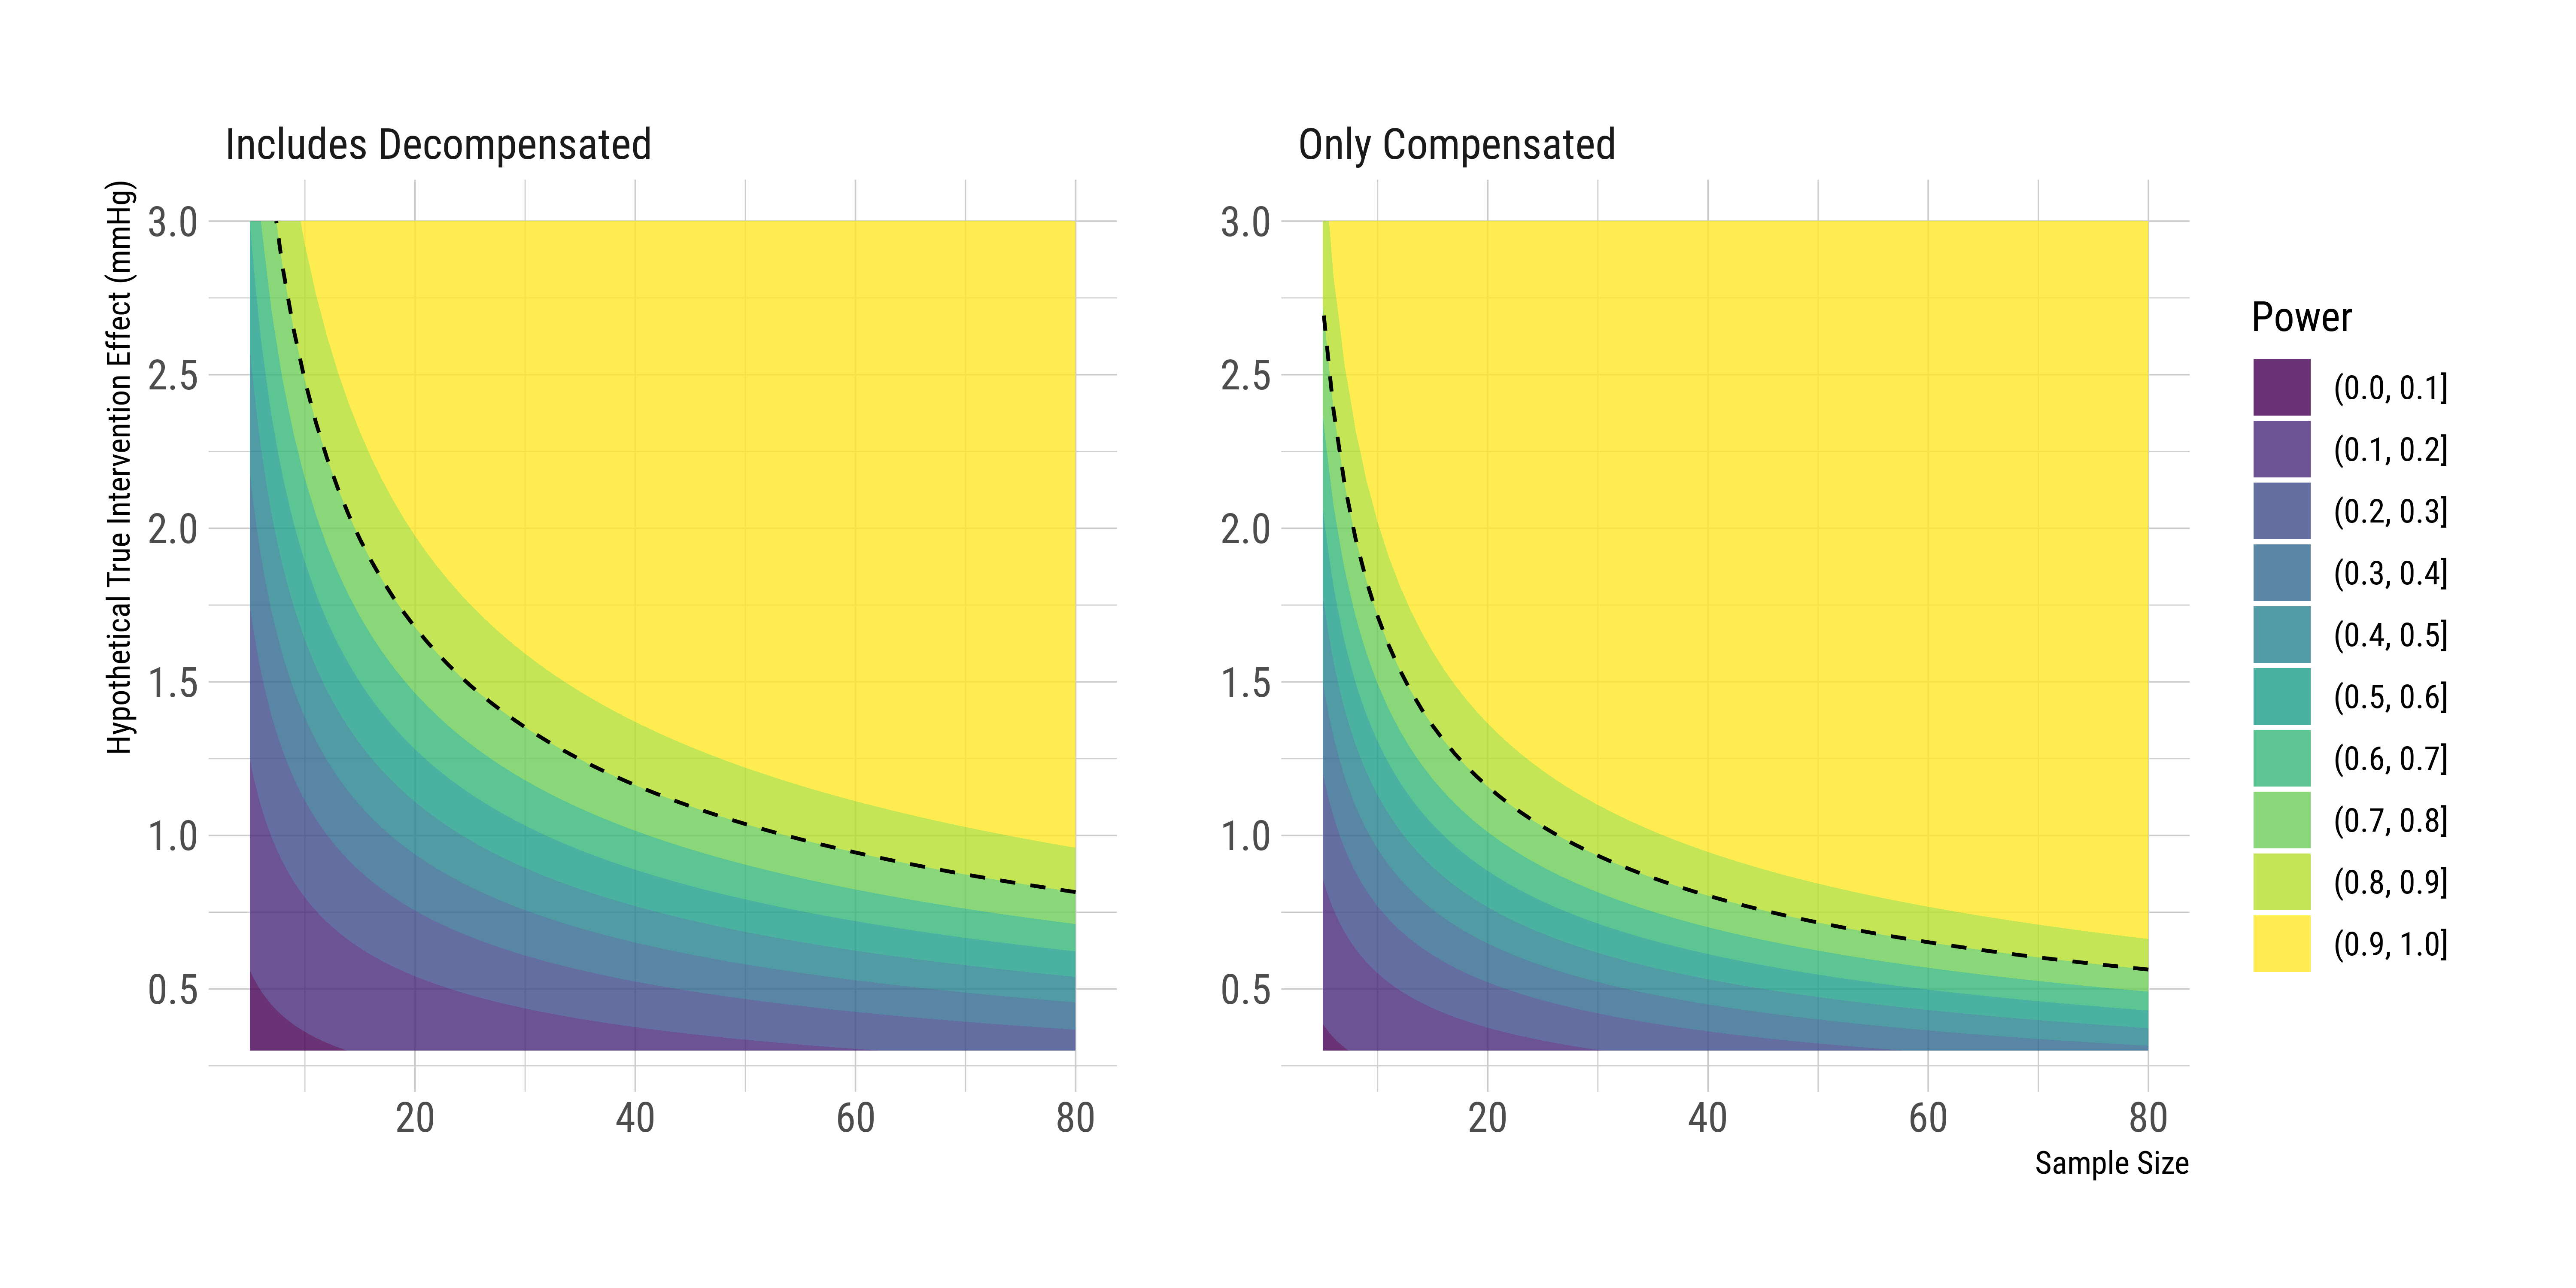
\includegraphics{figures/unnamed-chunk-61-1.png}

\hypertarget{required-individuals}{%
\subsection{Required Individuals}\label{required-individuals}}

And how many people do we need for each scenario?

\begin{Shaded}
\begin{Highlighting}[]
\NormalTok{difsims\_80power }\OtherTok{\textless{}{-}}\NormalTok{ difsims\_res }\SpecialCharTok{\%\textgreater{}\%} 
  \FunctionTok{arrange}\NormalTok{(power) }\SpecialCharTok{\%\textgreater{}\%} 
  \FunctionTok{filter}\NormalTok{(power }\SpecialCharTok{\textgreater{}} \FloatTok{0.8}\NormalTok{) }\SpecialCharTok{\%\textgreater{}\%} 
  \FunctionTok{select}\NormalTok{(decomp, delta, Effects, n) }\SpecialCharTok{\%\textgreater{}\%} 
  \FunctionTok{group\_by}\NormalTok{(delta, Effects, decomp) }\SpecialCharTok{\%\textgreater{}\%} 
  \FunctionTok{slice}\NormalTok{(}\DecValTok{1}\NormalTok{) }\SpecialCharTok{\%\textgreater{}\%} 
  \FunctionTok{arrange}\NormalTok{(decomp, delta) }\SpecialCharTok{\%\textgreater{}\%} 
  \FunctionTok{rename}\NormalTok{(}\StringTok{"Patients"} \OtherTok{=}\NormalTok{ decomp,}
         \StringTok{"Difference (mmHg)"} \OtherTok{=}\NormalTok{ delta,}
         \StringTok{"80\% Power"} \OtherTok{=}\NormalTok{ n)}

\NormalTok{difsims\_90power }\OtherTok{\textless{}{-}}\NormalTok{ difsims\_res }\SpecialCharTok{\%\textgreater{}\%} 
  \FunctionTok{arrange}\NormalTok{(power) }\SpecialCharTok{\%\textgreater{}\%} 
  \FunctionTok{filter}\NormalTok{(power }\SpecialCharTok{\textgreater{}} \FloatTok{0.9}\NormalTok{) }\SpecialCharTok{\%\textgreater{}\%} 
  \FunctionTok{select}\NormalTok{(decomp, delta, Effects, n) }\SpecialCharTok{\%\textgreater{}\%} 
  \FunctionTok{group\_by}\NormalTok{(delta, Effects, decomp) }\SpecialCharTok{\%\textgreater{}\%} 
  \FunctionTok{slice}\NormalTok{(}\DecValTok{1}\NormalTok{) }\SpecialCharTok{\%\textgreater{}\%} 
  \FunctionTok{arrange}\NormalTok{(decomp, delta) }\SpecialCharTok{\%\textgreater{}\%} 
  \FunctionTok{rename}\NormalTok{(}\StringTok{"Patients"} \OtherTok{=}\NormalTok{ decomp,}
         \StringTok{"Difference (mmHg)"} \OtherTok{=}\NormalTok{ delta,}
         \StringTok{"90\% Power"} \OtherTok{=}\NormalTok{ n)}

\NormalTok{difsims\_power }\OtherTok{\textless{}{-}} \FunctionTok{left\_join}\NormalTok{(difsims\_80power, difsims\_90power)}

\NormalTok{decomp\_change }\OtherTok{\textless{}{-}} \FunctionTok{head}\NormalTok{(}
  \FunctionTok{which}\NormalTok{(}
\NormalTok{    difsims\_power}\SpecialCharTok{$}\NormalTok{Patients }\SpecialCharTok{==}
\NormalTok{      trt\_all}\SpecialCharTok{$}\NormalTok{decomp[}\DecValTok{2}\NormalTok{]), }\DecValTok{1}\NormalTok{)}

\FunctionTok{kable}\NormalTok{(difsims\_power[,}\SpecialCharTok{{-}}\DecValTok{1}\NormalTok{]) }\SpecialCharTok{\%\textgreater{}\%} 
  \FunctionTok{kable\_styling}\NormalTok{(}\StringTok{"striped"}\NormalTok{, }\AttributeTok{full\_width =}\NormalTok{ F) }\SpecialCharTok{\%\textgreater{}\%}
  \FunctionTok{pack\_rows}\NormalTok{(trt\_all}\SpecialCharTok{$}\NormalTok{decomp[}\DecValTok{1}\NormalTok{], }\DecValTok{1}\NormalTok{, decomp\_change}\DecValTok{{-}1}\NormalTok{) }\SpecialCharTok{\%\textgreater{}\%}
  \FunctionTok{pack\_rows}\NormalTok{(trt\_all}\SpecialCharTok{$}\NormalTok{decomp[}\DecValTok{2}\NormalTok{], decomp\_change, }\FunctionTok{nrow}\NormalTok{(difsims\_80power))}
\end{Highlighting}
\end{Shaded}

\begin{table}[H]
\centering
\begin{tabular}{l|l|r|r}
\hline
Difference (mmHg) & Effects & 80\% Power & 90\% Power\\
\hline
\multicolumn{4}{l}{\textbf{Includes Decompensated}}\\
\hline
\hspace{1em}1 & Homogeneous Effects & 55 & 75\\
\hline
\hspace{1em}1 & Heterogeneous Effects & 60 & 80\\
\hline
\hspace{1em}1.5 & Homogeneous Effects & 25 & 35\\
\hline
\hspace{1em}1.5 & Heterogeneous Effects & 30 & 40\\
\hline
\hspace{1em}2 & Homogeneous Effects & 15 & 20\\
\hline
\hspace{1em}2 & Heterogeneous Effects & 20 & 25\\
\hline
\hspace{1em}2.5 & Homogeneous Effects & 10 & 15\\
\hline
\hspace{1em}2.5 & Heterogeneous Effects & 15 & 20\\
\hline
\hspace{1em}3 & Homogeneous Effects & 10 & 10\\
\hline
\hspace{1em}3 & Heterogeneous Effects & 10 & 15\\
\hline
\multicolumn{4}{l}{\textbf{Only Compensated}}\\
\hline
\hspace{1em}1 & Homogeneous Effects & 30 & 40\\
\hline
\hspace{1em}1 & Heterogeneous Effects & 30 & 40\\
\hline
\hspace{1em}1.5 & Homogeneous Effects & 15 & 20\\
\hline
\hspace{1em}1.5 & Heterogeneous Effects & 15 & 20\\
\hline
\hspace{1em}2 & Homogeneous Effects & 10 & 15\\
\hline
\hspace{1em}2 & Heterogeneous Effects & 10 & 15\\
\hline
\hspace{1em}2.5 & Homogeneous Effects & 10 & 10\\
\hline
\hspace{1em}2.5 & Heterogeneous Effects & 10 & 10\\
\hline
\hspace{1em}3 & Homogeneous Effects & 5 & 10\\
\hline
\hspace{1em}3 & Heterogeneous Effects & 10 & 10\\
\hline
\end{tabular}
\end{table}

\hypertarget{analytical-solution}{%
\subsection{Analytical solution}\label{analytical-solution}}

Let's compare these with the analytical solution

\begin{itemize}
\item
  Decomp
\item
  Homogeneous
\item
  1.5
\item
  Expect: 20 \textless{} n \textless{} 25
\end{itemize}

\begin{Shaded}
\begin{Highlighting}[]
\FunctionTok{library}\NormalTok{(pwr)}

\NormalTok{dz }\OtherTok{\textless{}{-}} \FloatTok{1.5}\SpecialCharTok{/}\NormalTok{(trt\_all}\SpecialCharTok{$}\NormalTok{signvar\_sd[}\DecValTok{1}\NormalTok{]}\SpecialCharTok{*}\NormalTok{trt\_all}\SpecialCharTok{$}\NormalTok{mean[}\DecValTok{1}\NormalTok{])}

\NormalTok{pwr}\SpecialCharTok{::}\FunctionTok{pwr.t.test}\NormalTok{(}\AttributeTok{d=}\NormalTok{dz, }\AttributeTok{sig.level =} \FloatTok{0.05}\NormalTok{, }\AttributeTok{power =} \FloatTok{0.8}\NormalTok{, }
                \AttributeTok{type =} \StringTok{"paired"}\NormalTok{, }\AttributeTok{alternative =} \StringTok{"greater"}\NormalTok{)}
\end{Highlighting}
\end{Shaded}

\begin{verbatim}
## 
##      Paired t test power calculation 
## 
##               n = 20.45661
##               d = 0.5699301
##       sig.level = 0.05
##           power = 0.8
##     alternative = greater
## 
## NOTE: n is number of *pairs*
\end{verbatim}

And hetero

\begin{itemize}
\item
  Decomp
\item
  Homogeneous
\item
  1.5
\item
  Expect: 25 \textless{} n \textless{} 30
\end{itemize}

\begin{Shaded}
\begin{Highlighting}[]
\NormalTok{signvar\_sd }\OtherTok{\textless{}{-}} \FunctionTok{sqrt}\NormalTok{(}
\NormalTok{    (trt\_all}\SpecialCharTok{$}\NormalTok{signvar\_sd[}\DecValTok{1}\NormalTok{]}\SpecialCharTok{*}\NormalTok{trt\_all}\SpecialCharTok{$}\NormalTok{mean[}\DecValTok{1}\NormalTok{])}\SpecialCharTok{\^{}}\DecValTok{2} \SpecialCharTok{+}
\NormalTok{    (}\FloatTok{0.5}\SpecialCharTok{*}\FloatTok{1.5}\NormalTok{)}\SpecialCharTok{\^{}}\DecValTok{2}\NormalTok{)}
  

\NormalTok{dz }\OtherTok{\textless{}{-}} \FloatTok{1.5}\SpecialCharTok{/}\NormalTok{signvar\_sd}

\NormalTok{pwr}\SpecialCharTok{::}\FunctionTok{pwr.t.test}\NormalTok{(}\AttributeTok{d=}\NormalTok{dz, }\AttributeTok{sig.level =} \FloatTok{0.05}\NormalTok{, }\AttributeTok{power =} \FloatTok{0.8}\NormalTok{, }
                \AttributeTok{type =} \StringTok{"paired"}\NormalTok{, }\AttributeTok{alternative =} \StringTok{"greater"}\NormalTok{)}
\end{Highlighting}
\end{Shaded}

\begin{verbatim}
## 
##      Paired t test power calculation 
## 
##               n = 21.99721
##               d = 0.5481097
##       sig.level = 0.05
##           power = 0.8
##     alternative = greater
## 
## NOTE: n is number of *pairs*
\end{verbatim}

\begin{Shaded}
\begin{Highlighting}[]
\NormalTok{difsims\_ana }\OtherTok{\textless{}{-}} \ControlFlowTok{function}\NormalTok{(Patients, Difference, Effects, Power,}
                        \AttributeTok{trt\_all=}\NormalTok{trt\_all) \{}
  
\NormalTok{  Effects }\OtherTok{\textless{}{-}} \FunctionTok{as.character}\NormalTok{(Effects)}
\NormalTok{  Difference }\OtherTok{\textless{}{-}} \FunctionTok{as.numeric}\NormalTok{(Difference)}
  
\NormalTok{  heterogen }\OtherTok{\textless{}{-}} \FunctionTok{ifelse}\NormalTok{(Effects}\SpecialCharTok{==}\StringTok{"Homogeneous Effects"}\NormalTok{,}
                      \DecValTok{0}\NormalTok{, }\FloatTok{0.5}\NormalTok{)}
  
\NormalTok{  decomp }\OtherTok{=} \FunctionTok{ifelse}\NormalTok{(Patients}\SpecialCharTok{==}\StringTok{"Includes Decompensated"}\NormalTok{, }\DecValTok{1}\NormalTok{, }\DecValTok{2}\NormalTok{)}
  
\NormalTok{  trt\_all\_pat }\OtherTok{\textless{}{-}}\NormalTok{ trt\_all[decomp,]}
  
\NormalTok{  signvar\_sd }\OtherTok{\textless{}{-}} \FunctionTok{sqrt}\NormalTok{(}
\NormalTok{    (trt\_all\_pat}\SpecialCharTok{$}\NormalTok{signvar\_sd}\SpecialCharTok{*}\NormalTok{trt\_all\_pat}\SpecialCharTok{$}\NormalTok{mean)}\SpecialCharTok{\^{}}\DecValTok{2} \SpecialCharTok{+}
\NormalTok{    (heterogen}\SpecialCharTok{*}\NormalTok{Difference)}\SpecialCharTok{\^{}}\DecValTok{2}\NormalTok{)}
  
\NormalTok{  dz }\OtherTok{\textless{}{-}}\NormalTok{ Difference}\SpecialCharTok{/}\NormalTok{signvar\_sd}
  
  \FunctionTok{ceiling}\NormalTok{(pwr}\SpecialCharTok{::}\FunctionTok{pwr.t.test}\NormalTok{(}\AttributeTok{d=}\NormalTok{dz, }\AttributeTok{sig.level =} \FloatTok{0.05}\NormalTok{, }\AttributeTok{power =}\NormalTok{ Power,}
                       \AttributeTok{alternative =} \StringTok{"greater"}\NormalTok{, }\AttributeTok{type =} \StringTok{"paired"}\NormalTok{)}\SpecialCharTok{$}\NormalTok{n)}
  
\NormalTok{\}}

\NormalTok{difsims\_power\_ana }\OtherTok{\textless{}{-}}\NormalTok{ difsims\_power }\SpecialCharTok{\%\textgreater{}\%} 
  \FunctionTok{rename}\NormalTok{(}\AttributeTok{Difference =} \StringTok{\textasciigrave{}}\AttributeTok{Difference (mmHg)}\StringTok{\textasciigrave{}}\NormalTok{) }\SpecialCharTok{\%\textgreater{}\%} 
  \FunctionTok{mutate}\NormalTok{(}\AttributeTok{Difference =} \FunctionTok{as.numeric}\NormalTok{(}\FunctionTok{as.character}\NormalTok{(Difference)),}
         \AttributeTok{Effects=} \FunctionTok{as.character}\NormalTok{(Effects)) }\SpecialCharTok{\%\textgreater{}\%} 
  \FunctionTok{group\_by}\NormalTok{(Patients, Difference, Effects) }\SpecialCharTok{\%\textgreater{}\%} 
  \FunctionTok{mutate}\NormalTok{(}\StringTok{"80\% Power"}\OtherTok{=} \FunctionTok{pmap\_dbl}\NormalTok{(}\FunctionTok{list}\NormalTok{(Patients, Difference,}
\NormalTok{                                    Effects), difsims\_ana, }\AttributeTok{Power=}\FloatTok{0.8}\NormalTok{,}
                                   \AttributeTok{trt\_all =}\NormalTok{ trt\_all),}
         \StringTok{"90\% Power"}\OtherTok{=} \FunctionTok{pmap\_dbl}\NormalTok{(}\FunctionTok{list}\NormalTok{(Patients, Difference,}
\NormalTok{                                    Effects), difsims\_ana, }\AttributeTok{Power=}\FloatTok{0.9}\NormalTok{,}
                                   \AttributeTok{trt\_all =}\NormalTok{ trt\_all))}

\FunctionTok{kable}\NormalTok{(difsims\_power\_ana[,}\SpecialCharTok{{-}}\DecValTok{1}\NormalTok{]) }\SpecialCharTok{\%\textgreater{}\%} 
  \FunctionTok{kable\_styling}\NormalTok{(}\StringTok{"striped"}\NormalTok{, }\AttributeTok{full\_width =}\NormalTok{ F) }\SpecialCharTok{\%\textgreater{}\%}
  \FunctionTok{pack\_rows}\NormalTok{(trt\_all}\SpecialCharTok{$}\NormalTok{decomp[}\DecValTok{1}\NormalTok{], }\DecValTok{1}\NormalTok{, decomp\_change}\DecValTok{{-}1}\NormalTok{) }\SpecialCharTok{\%\textgreater{}\%}
  \FunctionTok{pack\_rows}\NormalTok{(trt\_all}\SpecialCharTok{$}\NormalTok{decomp[}\DecValTok{2}\NormalTok{], decomp\_change, }\FunctionTok{nrow}\NormalTok{(difsims\_power\_ana))}
\end{Highlighting}
\end{Shaded}

\begin{table}[H]
\centering
\begin{tabular}{r|l|r|r}
\hline
Difference & Effects & 80\% Power & 90\% Power\\
\hline
\multicolumn{4}{l}{\textbf{Includes Decompensated}}\\
\hline
\hspace{1em}1.0 & Homogeneous Effects & 45 & 61\\
\hline
\hspace{1em}1.0 & Heterogeneous Effects & 46 & 63\\
\hline
\hspace{1em}1.5 & Homogeneous Effects & 21 & 28\\
\hline
\hspace{1em}1.5 & Heterogeneous Effects & 22 & 30\\
\hline
\hspace{1em}2.0 & Homogeneous Effects & 13 & 17\\
\hline
\hspace{1em}2.0 & Heterogeneous Effects & 14 & 19\\
\hline
\hspace{1em}2.5 & Homogeneous Effects & 9 & 11\\
\hline
\hspace{1em}2.5 & Heterogeneous Effects & 10 & 14\\
\hline
\hspace{1em}3.0 & Homogeneous Effects & 7 & 9\\
\hline
\hspace{1em}3.0 & Heterogeneous Effects & 8 & 11\\
\hline
\multicolumn{4}{l}{\textbf{Only Compensated}}\\
\hline
\hspace{1em}1.0 & Homogeneous Effects & 32 & 43\\
\hline
\hspace{1em}1.0 & Heterogeneous Effects & 33 & 45\\
\hline
\hspace{1em}1.5 & Homogeneous Effects & 15 & 20\\
\hline
\hspace{1em}1.5 & Heterogeneous Effects & 17 & 22\\
\hline
\hspace{1em}2.0 & Homogeneous Effects & 9 & 12\\
\hline
\hspace{1em}2.0 & Heterogeneous Effects & 11 & 14\\
\hline
\hspace{1em}2.5 & Homogeneous Effects & 7 & 9\\
\hline
\hspace{1em}2.5 & Heterogeneous Effects & 8 & 11\\
\hline
\hspace{1em}3.0 & Homogeneous Effects & 5 & 7\\
\hline
\hspace{1em}3.0 & Heterogeneous Effects & 7 & 9\\
\hline
\end{tabular}
\end{table}

\begin{Shaded}
\begin{Highlighting}[]
\NormalTok{difpower }\OtherTok{\textless{}{-}} \FunctionTok{kable}\NormalTok{(difsims\_power\_ana[,}\SpecialCharTok{{-}}\DecValTok{1}\NormalTok{]) }\SpecialCharTok{\%\textgreater{}\%} 
  \FunctionTok{kable\_styling}\NormalTok{(}\StringTok{"striped"}\NormalTok{, }\AttributeTok{full\_width =}\NormalTok{ F) }\SpecialCharTok{\%\textgreater{}\%}
  \FunctionTok{pack\_rows}\NormalTok{(trt\_all}\SpecialCharTok{$}\NormalTok{decomp[}\DecValTok{1}\NormalTok{], }\DecValTok{1}\NormalTok{, decomp\_change}\DecValTok{{-}1}\NormalTok{) }\SpecialCharTok{\%\textgreater{}\%}
  \FunctionTok{pack\_rows}\NormalTok{(trt\_all}\SpecialCharTok{$}\NormalTok{decomp[}\DecValTok{2}\NormalTok{], decomp\_change, }\FunctionTok{nrow}\NormalTok{(difsims\_power\_ana))}

\NormalTok{difpower}
\end{Highlighting}
\end{Shaded}

\begin{table}[H]
\centering
\begin{tabular}{r|l|r|r}
\hline
Difference & Effects & 80\% Power & 90\% Power\\
\hline
\multicolumn{4}{l}{\textbf{Includes Decompensated}}\\
\hline
\hspace{1em}1.0 & Homogeneous Effects & 45 & 61\\
\hline
\hspace{1em}1.0 & Heterogeneous Effects & 46 & 63\\
\hline
\hspace{1em}1.5 & Homogeneous Effects & 21 & 28\\
\hline
\hspace{1em}1.5 & Heterogeneous Effects & 22 & 30\\
\hline
\hspace{1em}2.0 & Homogeneous Effects & 13 & 17\\
\hline
\hspace{1em}2.0 & Heterogeneous Effects & 14 & 19\\
\hline
\hspace{1em}2.5 & Homogeneous Effects & 9 & 11\\
\hline
\hspace{1em}2.5 & Heterogeneous Effects & 10 & 14\\
\hline
\hspace{1em}3.0 & Homogeneous Effects & 7 & 9\\
\hline
\hspace{1em}3.0 & Heterogeneous Effects & 8 & 11\\
\hline
\multicolumn{4}{l}{\textbf{Only Compensated}}\\
\hline
\hspace{1em}1.0 & Homogeneous Effects & 32 & 43\\
\hline
\hspace{1em}1.0 & Heterogeneous Effects & 33 & 45\\
\hline
\hspace{1em}1.5 & Homogeneous Effects & 15 & 20\\
\hline
\hspace{1em}1.5 & Heterogeneous Effects & 17 & 22\\
\hline
\hspace{1em}2.0 & Homogeneous Effects & 9 & 12\\
\hline
\hspace{1em}2.0 & Heterogeneous Effects & 11 & 14\\
\hline
\hspace{1em}2.5 & Homogeneous Effects & 7 & 9\\
\hline
\hspace{1em}2.5 & Heterogeneous Effects & 8 & 11\\
\hline
\hspace{1em}3.0 & Homogeneous Effects & 5 & 7\\
\hline
\hspace{1em}3.0 & Heterogeneous Effects & 7 & 9\\
\hline
\end{tabular}
\end{table}

\begin{Shaded}
\begin{Highlighting}[]
\CommentTok{\# save\_kable(difpower, "figures/difpower.jpg")}
\end{Highlighting}
\end{Shaded}

\hypertarget{contour-plots}{%
\subsubsection{Contour Plots}\label{contour-plots}}

\begin{Shaded}
\begin{Highlighting}[]
\NormalTok{difsims\_ana\_contour }\OtherTok{\textless{}{-}} \ControlFlowTok{function}\NormalTok{(Patients, Difference, Effects, n,}
                        \AttributeTok{trt\_all=}\NormalTok{trt\_all) \{}
  
\NormalTok{  Effects }\OtherTok{\textless{}{-}} \FunctionTok{as.character}\NormalTok{(Effects)}
\NormalTok{  Difference }\OtherTok{\textless{}{-}} \FunctionTok{as.numeric}\NormalTok{(Difference)}
  
\NormalTok{  heterogen }\OtherTok{\textless{}{-}} \FunctionTok{ifelse}\NormalTok{(Effects}\SpecialCharTok{==}\StringTok{"Homogeneous Effects"}\NormalTok{,}
                      \DecValTok{0}\NormalTok{, }\FloatTok{0.5}\NormalTok{)}
  
\NormalTok{  decomp }\OtherTok{=} \FunctionTok{ifelse}\NormalTok{(Patients}\SpecialCharTok{==}\StringTok{"Includes Decompensated"}\NormalTok{, }\DecValTok{1}\NormalTok{, }\DecValTok{2}\NormalTok{)}
  
\NormalTok{  trt\_all\_pat }\OtherTok{\textless{}{-}}\NormalTok{ trt\_all[decomp,]}
  
\NormalTok{  signvar\_sd }\OtherTok{\textless{}{-}} \FunctionTok{sqrt}\NormalTok{(}
\NormalTok{    (trt\_all\_pat}\SpecialCharTok{$}\NormalTok{signvar\_sd}\SpecialCharTok{*}\NormalTok{trt\_all\_pat}\SpecialCharTok{$}\NormalTok{mean)}\SpecialCharTok{\^{}}\DecValTok{2} \SpecialCharTok{+}
\NormalTok{    (heterogen}\SpecialCharTok{*}\NormalTok{Difference)}\SpecialCharTok{\^{}}\DecValTok{2}\NormalTok{)}
  
\NormalTok{  dz }\OtherTok{\textless{}{-}}\NormalTok{ Difference}\SpecialCharTok{/}\NormalTok{signvar\_sd}
  
\NormalTok{  pwr}\SpecialCharTok{::}\FunctionTok{pwr.t.test}\NormalTok{(}\AttributeTok{d=}\NormalTok{dz, }\AttributeTok{sig.level =} \FloatTok{0.05}\NormalTok{, }\AttributeTok{n =}\NormalTok{ n,}
                       \AttributeTok{alternative =} \StringTok{"greater"}\NormalTok{, }\AttributeTok{type =} \StringTok{"paired"}\NormalTok{)}\SpecialCharTok{$}\NormalTok{power}
  
\NormalTok{\}}

\NormalTok{contour\_dat }\OtherTok{\textless{}{-}}\NormalTok{ tidyr}\SpecialCharTok{::}\FunctionTok{crossing}\NormalTok{(}\AttributeTok{Difference =} \FunctionTok{seq}\NormalTok{(}\FloatTok{0.3}\NormalTok{,}\DecValTok{3}\NormalTok{,}\AttributeTok{length.out=}\DecValTok{2701}\NormalTok{),}
                               \AttributeTok{n =} \DecValTok{5}\SpecialCharTok{:}\DecValTok{80}\NormalTok{,}
                               \AttributeTok{Effects =} \FunctionTok{c}\NormalTok{(}\StringTok{"Homogeneous Effects"}\NormalTok{, }
                                           \StringTok{"Heterogeneous Effects"}\NormalTok{),}
                               \AttributeTok{Patients =} \FunctionTok{c}\NormalTok{(}\StringTok{"Includes Decompensated"}\NormalTok{, }
                                            \StringTok{"Only Compensated"}\NormalTok{))}
\end{Highlighting}
\end{Shaded}

Run it

\begin{Shaded}
\begin{Highlighting}[]
\NormalTok{contour\_power }\OtherTok{\textless{}{-}}\NormalTok{ contour\_dat }\SpecialCharTok{\%\textgreater{}\%} 
  \FunctionTok{mutate}\NormalTok{(}\AttributeTok{Test =} \DecValTok{1}\SpecialCharTok{:}\FunctionTok{n}\NormalTok{()) }\SpecialCharTok{\%\textgreater{}\%} 
  \FunctionTok{group\_by}\NormalTok{(Test) }\SpecialCharTok{\%\textgreater{}\%} 
  \FunctionTok{mutate}\NormalTok{(}\AttributeTok{Power=}\FunctionTok{pmap\_dbl}\NormalTok{(}\FunctionTok{list}\NormalTok{(Patients, Difference, Effects, n), }
\NormalTok{                        difsims\_ana\_contour, }\AttributeTok{trt\_all=}\NormalTok{trt\_all)) }\SpecialCharTok{\%\textgreater{}\%} 
  \FunctionTok{ungroup}\NormalTok{()}

\FunctionTok{saveRDS}\NormalTok{(contour\_power, }\StringTok{"../DerivedData/contour\_power.rds"}\NormalTok{)}
\end{Highlighting}
\end{Shaded}

\begin{Shaded}
\begin{Highlighting}[]
\NormalTok{contour\_power }\OtherTok{\textless{}{-}} \FunctionTok{readRDS}\NormalTok{(}\StringTok{"../DerivedData/contour\_power.rds"}\NormalTok{)}

\FunctionTok{library}\NormalTok{(viridis)}

\NormalTok{contour\_power }\OtherTok{\textless{}{-}}\NormalTok{ contour\_power }\SpecialCharTok{\%\textgreater{}\%} 
  \FunctionTok{mutate}\NormalTok{(}\AttributeTok{Power\_cut =} \FunctionTok{cut}\NormalTok{(Power, }\AttributeTok{breaks =} \FunctionTok{seq}\NormalTok{(}\DecValTok{0}\NormalTok{,}\DecValTok{1}\NormalTok{, }\AttributeTok{length.out =} \DecValTok{11}\NormalTok{))) }\SpecialCharTok{\%\textgreater{}\%} 
  \FunctionTok{mutate}\NormalTok{(}\AttributeTok{Power =} \FunctionTok{ifelse}\NormalTok{(Power }\SpecialCharTok{==} \DecValTok{1}\NormalTok{, }\FloatTok{0.99}\NormalTok{, Power)) }\CommentTok{\# Note below to explain this}
                                                  

\NormalTok{contour\_het }\OtherTok{\textless{}{-}}\NormalTok{ contour\_power }\SpecialCharTok{\%\textgreater{}\%} 
  \FunctionTok{filter}\NormalTok{(Effects}\SpecialCharTok{!=}\StringTok{"Homogeneous Effects"}\NormalTok{)}

\NormalTok{contour\_hom }\OtherTok{\textless{}{-}}\NormalTok{ contour\_power }\SpecialCharTok{\%\textgreater{}\%} 
  \FunctionTok{filter}\NormalTok{(Effects}\SpecialCharTok{==}\StringTok{"Homogeneous Effects"}\NormalTok{)}


\NormalTok{homplot }\OtherTok{\textless{}{-}} \FunctionTok{ggplot}\NormalTok{(contour\_hom, }\FunctionTok{aes}\NormalTok{(}\AttributeTok{x=}\NormalTok{n, }\AttributeTok{y=}\NormalTok{Difference, }\AttributeTok{z=}\NormalTok{Power)) }\SpecialCharTok{+}
  \FunctionTok{geom\_contour\_filled}\NormalTok{(}\AttributeTok{alpha=}\FloatTok{0.8}\NormalTok{, }\AttributeTok{breaks=}\FunctionTok{seq}\NormalTok{(}\DecValTok{0}\NormalTok{,}\DecValTok{1}\NormalTok{, }\AttributeTok{by=}\FloatTok{0.1}\NormalTok{)) }\SpecialCharTok{+}
  \FunctionTok{facet\_wrap}\NormalTok{(.}\SpecialCharTok{\textasciitilde{}}\NormalTok{Patients, }\AttributeTok{scales =} \StringTok{"free"}\NormalTok{) }\SpecialCharTok{+}
  \FunctionTok{theme\_ipsum\_rc}\NormalTok{() }\SpecialCharTok{+}
  \FunctionTok{labs}\NormalTok{(}\AttributeTok{x =} \StringTok{"Sample Size"}\NormalTok{,}
       \AttributeTok{y =} \StringTok{"Hypothetical True Intervention Effect (mmHg)"}\NormalTok{) }\SpecialCharTok{+}
  \FunctionTok{scale\_y\_continuous}\NormalTok{(}\AttributeTok{breaks =} \FunctionTok{seq}\NormalTok{(}\FloatTok{0.5}\NormalTok{, }\DecValTok{3}\NormalTok{, }\AttributeTok{by =} \FloatTok{0.5}\NormalTok{)) }\SpecialCharTok{+}
  \FunctionTok{scale\_fill\_viridis}\NormalTok{(}\StringTok{"Power"}\NormalTok{, }\AttributeTok{discrete =}\NormalTok{ T) }\SpecialCharTok{+}
  \FunctionTok{geom\_contour}\NormalTok{(}\AttributeTok{breaks=}\FloatTok{0.8}\NormalTok{, }\AttributeTok{colour=}\StringTok{"black"}\NormalTok{, }\AttributeTok{linetype=}\StringTok{"dashed"}\NormalTok{)}


\NormalTok{hetplot }\OtherTok{\textless{}{-}} \FunctionTok{ggplot}\NormalTok{(contour\_het, }\FunctionTok{aes}\NormalTok{(}\AttributeTok{x=}\NormalTok{n, }\AttributeTok{y=}\NormalTok{Difference, }\AttributeTok{z=}\NormalTok{Power)) }\SpecialCharTok{+}
  \FunctionTok{geom\_contour\_filled}\NormalTok{(}\AttributeTok{alpha=}\FloatTok{0.8}\NormalTok{, }\AttributeTok{breaks=}\FunctionTok{seq}\NormalTok{(}\DecValTok{0}\NormalTok{,}\FloatTok{1.1}\NormalTok{, }\AttributeTok{by=}\FloatTok{0.1}\NormalTok{)) }\SpecialCharTok{+}
  \FunctionTok{facet\_wrap}\NormalTok{(.}\SpecialCharTok{\textasciitilde{}}\NormalTok{Patients, }\AttributeTok{scales =} \StringTok{"free"}\NormalTok{) }\SpecialCharTok{+}
  \FunctionTok{theme\_ipsum\_rc}\NormalTok{() }\SpecialCharTok{+}
  \FunctionTok{labs}\NormalTok{(}\AttributeTok{x =} \StringTok{"Sample Size"}\NormalTok{,}
       \AttributeTok{y =} \StringTok{"Hypothetical True Intervention Effect (mmHg)"}\NormalTok{) }\SpecialCharTok{+}
  \FunctionTok{scale\_y\_continuous}\NormalTok{(}\AttributeTok{breaks =} \FunctionTok{seq}\NormalTok{(}\FloatTok{0.5}\NormalTok{, }\DecValTok{3}\NormalTok{, }\AttributeTok{by =} \FloatTok{0.5}\NormalTok{)) }\SpecialCharTok{+}
  \FunctionTok{scale\_fill\_viridis}\NormalTok{(}\StringTok{"Power"}\NormalTok{, }\AttributeTok{discrete =}\NormalTok{ T) }\SpecialCharTok{+}
  \FunctionTok{geom\_contour}\NormalTok{(}\AttributeTok{breaks=}\FloatTok{0.8}\NormalTok{, }\AttributeTok{colour=}\StringTok{"black"}\NormalTok{, }\AttributeTok{linetype=}\StringTok{"dashed"}\NormalTok{)}

\NormalTok{homplot}
\end{Highlighting}
\end{Shaded}

\includegraphics{figures/unnamed-chunk-68-1.png}

\begin{Shaded}
\begin{Highlighting}[]
\NormalTok{hetplot}
\end{Highlighting}
\end{Shaded}

\includegraphics{figures/unnamed-chunk-68-2.png}

\begin{Shaded}
\begin{Highlighting}[]
\FunctionTok{ggsave}\NormalTok{(homplot, }\AttributeTok{height=}\DecValTok{5}\NormalTok{, }\AttributeTok{width=}\DecValTok{10}\NormalTok{, }\AttributeTok{filename =} \StringTok{"figures/Dif\_hom\_contour.png"}\NormalTok{)}
\FunctionTok{ggsave}\NormalTok{(hetplot, }\AttributeTok{height=}\DecValTok{5}\NormalTok{, }\AttributeTok{width=}\DecValTok{10}\NormalTok{, }\AttributeTok{filename =} \StringTok{"figures/Dif\_het\_contour.png"}\NormalTok{)}

\FunctionTok{ggsave}\NormalTok{(homplot, }\AttributeTok{height=}\DecValTok{5}\NormalTok{, }\AttributeTok{width=}\DecValTok{10}\NormalTok{, }\AttributeTok{filename =} \StringTok{"figures/Dif\_hom\_contour.jpg"}\NormalTok{, }
       \AttributeTok{dpi =} \DecValTok{600}\NormalTok{)}
\FunctionTok{ggsave}\NormalTok{(hetplot, }\AttributeTok{height=}\DecValTok{5}\NormalTok{, }\AttributeTok{width=}\DecValTok{10}\NormalTok{, }\AttributeTok{filename =} \StringTok{"figures/Dif\_het\_contour.jpg"}\NormalTok{, }
       \AttributeTok{dpi =} \DecValTok{600}\NormalTok{)}

\CommentTok{\# +}
\CommentTok{\#   xlab("Minor allele frequency")+}
\CommentTok{\#   ylab("Hypothetical effect size")+}
\CommentTok{\#   scale\_x\_log10(expand = c(0, 0), position = "bottom") +}
\CommentTok{\#   scale\_y\_continuous(expand = c(0, 0))+}
\CommentTok{\#   geom\_line(data = power.80, col = "black")+}
\CommentTok{\#   theme\_classic(base\_size = 12)}
\end{Highlighting}
\end{Shaded}

The strange line of code where I convert those values = 1 to 0.99 is to
prevent the graph from showing strangely. I think this has to do with
floating point accuracy. Some of the values equal to 1, are rounded in
the computer number system to a little bit above 1, and then the plot
makes them white. So by setting them to 0.99, they're still the same
colour, but the plot is filled correctly.

\hypertarget{power-analysis-for-difference-in-differences}{%
\section{Power Analysis for Difference in
Differences}\label{power-analysis-for-difference-in-differences}}

\hypertarget{simulation-1}{%
\subsection{Simulation}\label{simulation-1}}

\begin{Shaded}
\begin{Highlighting}[]
\NormalTok{HVPG\_difindif\_sim }\OtherTok{\textless{}{-}} \ControlFlowTok{function}\NormalTok{(n, delta1, delta2, cv\_delta, }
                              \AttributeTok{wscv=}\NormalTok{trt\_all}\SpecialCharTok{$}\NormalTok{wscv, }
                              \AttributeTok{mean=}\NormalTok{trt\_all}\SpecialCharTok{$}\NormalTok{mean, }
                              \AttributeTok{cv=}\NormalTok{trt\_all}\SpecialCharTok{$}\NormalTok{cv, }
\NormalTok{                              decomp ) \{}
  
\NormalTok{  wscv }\OtherTok{\textless{}{-}}\NormalTok{ wscv[decomp]}
\NormalTok{  mean }\OtherTok{\textless{}{-}}\NormalTok{ mean[decomp]}
\NormalTok{  cv   }\OtherTok{\textless{}{-}}\NormalTok{ cv[decomp]}
  
\NormalTok{  var }\OtherTok{\textless{}{-}}\NormalTok{ (cv}\SpecialCharTok{*}\NormalTok{mean)}\SpecialCharTok{\^{}}\DecValTok{2}
\NormalTok{  sd\_true }\OtherTok{\textless{}{-}} \FunctionTok{sqrt}\NormalTok{(var }\SpecialCharTok{*}\NormalTok{ icc)}
  
\NormalTok{  pre\_true1 }\OtherTok{\textless{}{-}} \FunctionTok{rnorm}\NormalTok{(n, mean, sd\_true)}
\NormalTok{  pre\_true2 }\OtherTok{\textless{}{-}} \FunctionTok{rnorm}\NormalTok{(n, mean, sd\_true)}
  
\NormalTok{  pre\_meas1 }\OtherTok{\textless{}{-}}\NormalTok{ pre\_true1 }\SpecialCharTok{+} \FunctionTok{rnorm}\NormalTok{(n, }\DecValTok{0}\NormalTok{, mean}\SpecialCharTok{*}\NormalTok{wscv)}
\NormalTok{  pre\_meas2 }\OtherTok{\textless{}{-}}\NormalTok{ pre\_true2 }\SpecialCharTok{+} \FunctionTok{rnorm}\NormalTok{(n, }\DecValTok{0}\NormalTok{, mean}\SpecialCharTok{*}\NormalTok{wscv)}
  
\NormalTok{  post\_true1 }\OtherTok{\textless{}{-}}\NormalTok{ pre\_true1 }\SpecialCharTok{{-}} \FunctionTok{rnorm}\NormalTok{(n, delta1, cv\_delta}\SpecialCharTok{*}\NormalTok{delta1)}
\NormalTok{  post\_true2 }\OtherTok{\textless{}{-}}\NormalTok{ pre\_true2 }\SpecialCharTok{{-}} \FunctionTok{rnorm}\NormalTok{(n, delta2, cv\_delta}\SpecialCharTok{*}\NormalTok{delta2)}
  
\NormalTok{  post\_meas1 }\OtherTok{\textless{}{-}}\NormalTok{ post\_true1 }\SpecialCharTok{+} \FunctionTok{rnorm}\NormalTok{(n, }\DecValTok{0}\NormalTok{, mean}\SpecialCharTok{*}\NormalTok{wscv)}
\NormalTok{  post\_meas2 }\OtherTok{\textless{}{-}}\NormalTok{ post\_true2 }\SpecialCharTok{+} \FunctionTok{rnorm}\NormalTok{(n, }\DecValTok{0}\NormalTok{, mean}\SpecialCharTok{*}\NormalTok{wscv)}
  
\NormalTok{  measured }\OtherTok{\textless{}{-}}\NormalTok{ tibble}\SpecialCharTok{::}\FunctionTok{tibble}\NormalTok{(}
    \AttributeTok{ID =} \FunctionTok{rep}\NormalTok{(}\DecValTok{1}\SpecialCharTok{:}\NormalTok{n, }\AttributeTok{times=}\DecValTok{2}\NormalTok{),}
    \AttributeTok{Pre =} \FunctionTok{c}\NormalTok{(pre\_meas1, pre\_meas2),}
    \AttributeTok{Post =} \FunctionTok{c}\NormalTok{(post\_meas1, post\_meas2),}
    \AttributeTok{Diff =}\NormalTok{ Post }\SpecialCharTok{{-}}\NormalTok{ Pre,}
    \AttributeTok{Group =} \FunctionTok{rep}\NormalTok{(}\FunctionTok{c}\NormalTok{(}\StringTok{"A"}\NormalTok{, }\StringTok{"B"}\NormalTok{), }\AttributeTok{each=}\NormalTok{n)}
\NormalTok{  )}
  
\NormalTok{  d }\OtherTok{\textless{}{-}}\NormalTok{ effsize}\SpecialCharTok{::}\FunctionTok{cohen.d}\NormalTok{(measured}\SpecialCharTok{$}\NormalTok{Diff, measured}\SpecialCharTok{$}\NormalTok{Group, }
                        \AttributeTok{paired=}\ConstantTok{FALSE}\NormalTok{)}\SpecialCharTok{$}\NormalTok{estimate}
  
\NormalTok{  mod }\OtherTok{\textless{}{-}} \FunctionTok{lm}\NormalTok{(Post }\SpecialCharTok{\textasciitilde{}}\NormalTok{ Pre }\SpecialCharTok{+}\NormalTok{ Group, }\AttributeTok{data=}\NormalTok{measured)}
  
\NormalTok{  testout }\OtherTok{\textless{}{-}}\NormalTok{ broom}\SpecialCharTok{::}\FunctionTok{tidy}\NormalTok{(mod) }\SpecialCharTok{\%\textgreater{}\%} 
    \FunctionTok{filter}\NormalTok{(term}\SpecialCharTok{==}\StringTok{"GroupB"}\NormalTok{) }\SpecialCharTok{\%\textgreater{}\%} 
    \FunctionTok{select}\NormalTok{(}\SpecialCharTok{{-}}\NormalTok{term) }\SpecialCharTok{\%\textgreater{}\%} 
    \FunctionTok{mutate}\NormalTok{(}\AttributeTok{p.value =} \FunctionTok{pt}\NormalTok{(statistic, mod}\SpecialCharTok{$}\NormalTok{df, }\AttributeTok{lower.tail =} \ConstantTok{FALSE}\NormalTok{))}
  \CommentTok{\# Note: using a one{-}sided p value}
  
\NormalTok{  out }\OtherTok{\textless{}{-}} \FunctionTok{mutate}\NormalTok{(testout, }\AttributeTok{d=}\NormalTok{d)}
  
  \FunctionTok{return}\NormalTok{(out)}
  
\NormalTok{\}}
\end{Highlighting}
\end{Shaded}

Now, we set up the simulation for various scenarios.

\begin{Shaded}
\begin{Highlighting}[]
\NormalTok{difindifsimpars }\OtherTok{\textless{}{-}}\NormalTok{ tidyr}\SpecialCharTok{::}\FunctionTok{crossing}\NormalTok{(}
  \AttributeTok{n =} \FunctionTok{c}\NormalTok{( }\FunctionTok{seq}\NormalTok{(}\DecValTok{5}\NormalTok{, }\DecValTok{100}\NormalTok{, }\AttributeTok{by =} \DecValTok{5}\NormalTok{), }\FunctionTok{seq}\NormalTok{(}\DecValTok{110}\NormalTok{, }\DecValTok{200}\NormalTok{, }\AttributeTok{by=}\DecValTok{10}\NormalTok{)),}
  \AttributeTok{delta1 =} \FunctionTok{seq}\NormalTok{(}\DecValTok{1}\NormalTok{,}\DecValTok{3}\NormalTok{, }\AttributeTok{by =} \FloatTok{0.5}\NormalTok{),}
  \AttributeTok{delta2 =} \FunctionTok{seq}\NormalTok{(}\DecValTok{0}\NormalTok{,}\DecValTok{2}\NormalTok{, }\AttributeTok{by =} \FloatTok{0.5}\NormalTok{),}
  \AttributeTok{cv\_delta =} \FunctionTok{c}\NormalTok{(}\DecValTok{0}\NormalTok{, }\FloatTok{0.5}\NormalTok{),}
\NormalTok{) }\SpecialCharTok{\%\textgreater{}\%} 
  \FunctionTok{mutate}\NormalTok{(}\AttributeTok{deltadif =}\NormalTok{ delta1 }\SpecialCharTok{{-}}\NormalTok{ delta2) }\SpecialCharTok{\%\textgreater{}\%} 
  \FunctionTok{filter}\NormalTok{(delta1 }\SpecialCharTok{\textgreater{}}\NormalTok{ delta2)}
\end{Highlighting}
\end{Shaded}

And we run it

\begin{Shaded}
\begin{Highlighting}[]
\CommentTok{\# if(!file.exists(paste0("../DerivedData/difindifsims\_decomp\_", }
\CommentTok{\#                        nsims, ".rds")) || overwrite) \{}
\CommentTok{\#   }
\CommentTok{\#   pb \textless{}{-} progress\_bar$new(total = nrow(difindifsimpars))}
\CommentTok{\#   }
\CommentTok{\#   difindifsims \textless{}{-} difindifsimpars \%\textgreater{}\% }
\CommentTok{\#     mutate(sim = 1:nrow(difindifsimpars)) \%\textgreater{}\% }
\CommentTok{\#     group\_by(sim) \%\textgreater{}\% }
\CommentTok{\#     nest(params = c(n, delta1, delta2, cv\_delta)) \%\textgreater{}\% }
\CommentTok{\#     mutate(output = map(params, .progress = TRUE,}
\CommentTok{\#                         \textasciitilde{}\{pb$tick(); }
\CommentTok{\#                           bind\_rows(purrr::rerun(nsims, }
\CommentTok{\#                           HVPG\_difindif\_sim(.x$n, .x$delta1, }
\CommentTok{\#                                             .x$delta2, .x$cv\_delta, }
\CommentTok{\#                                             decomp = 1)))\}))}
\CommentTok{\#   }
\CommentTok{\#   saveRDS(difindifsims, }
\CommentTok{\#           paste0("../DerivedData/difindifsims\_decomp\_", nsims, ".rds"))}
\CommentTok{\#   }
\CommentTok{\# \}}
\end{Highlighting}
\end{Shaded}

\begin{Shaded}
\begin{Highlighting}[]
\CommentTok{\# if(!file.exists(paste0("../DerivedData/difindifsims\_comp\_", }
\CommentTok{\#                        nsims, ".rds")) || overwrite) \{}
\CommentTok{\#   }
\CommentTok{\#   pb \textless{}{-} progress\_bar$new(total = nrow(difindifsimpars))}
\CommentTok{\#   }
\CommentTok{\#   difindifsims \textless{}{-} difindifsimpars \%\textgreater{}\% }
\CommentTok{\#     mutate(sim = 1:nrow(difindifsimpars)) \%\textgreater{}\% }
\CommentTok{\#     group\_by(sim) \%\textgreater{}\% }
\CommentTok{\#     nest(params = c(n, delta1, delta2, cv\_delta)) \%\textgreater{}\% }
\CommentTok{\#     mutate(output = map(params, }
\CommentTok{\#                         \textasciitilde{}\{pb$tick(); }
\CommentTok{\#                           bind\_rows(purrr::rerun(nsims, }
\CommentTok{\#                           HVPG\_difindif\_sim(.x$n, .x$delta1, }
\CommentTok{\#                                             .x$delta2, .x$cv\_delta,}
\CommentTok{\#                                             decomp = 2)))\}))}
\CommentTok{\#   }
\CommentTok{\#   saveRDS(difindifsims, }
\CommentTok{\#           paste0("../DerivedData/difindifsims\_comp\_", nsims, ".rds"))}
\CommentTok{\#   }
\CommentTok{\# \}}
\end{Highlighting}
\end{Shaded}

\begin{Shaded}
\begin{Highlighting}[]
\CommentTok{\# difindifsims\_decomp \textless{}{-} readRDS(paste0("../DerivedData/difindifsims\_decomp\_", nsims, ".rds"))}
\CommentTok{\# }
\CommentTok{\# difindifsims\_decomp\_res \textless{}{-} difindifsims\_decomp \%\textgreater{}\% }
\CommentTok{\#   ungroup() \%\textgreater{}\% }
\CommentTok{\#   mutate(power = map\_dbl(output, \textasciitilde{}mean(.x$p.value \textless{} 0.05))) \%\textgreater{}\% }
\CommentTok{\#   unnest(params) \%\textgreater{}\% }
\CommentTok{\#   mutate(deltadif = delta1 {-} delta2,}
\CommentTok{\#          delta1 = as.factor(delta1),}
\CommentTok{\#          delta2 = as.factor(delta2),}
\CommentTok{\#          deltadif = as.factor(deltadif)) \%\textgreater{}\% }
\CommentTok{\#   \#filter(deltadif != 0.5) \%\textgreater{}\% }
\CommentTok{\#   mutate(Effects = ifelse(cv\_delta==0, "Homogeneous Effects", }
\CommentTok{\#                                        "Heterogeneous Effects")) \%\textgreater{}\% }
\CommentTok{\#   mutate(Effects = fct\_inorder(Effects)) \%\textgreater{}\% }
\CommentTok{\#   mutate(decomp = trt\_all$decomp[1])}
\CommentTok{\# }
\CommentTok{\# }
\CommentTok{\# difindifsims\_comp \textless{}{-} readRDS(paste0("../DerivedData/difindifsims\_comp\_", nsims, ".rds"))}
\CommentTok{\# }
\CommentTok{\# difindifsims\_comp\_res \textless{}{-} difindifsims\_comp \%\textgreater{}\% }
\CommentTok{\#   ungroup() \%\textgreater{}\% }
\CommentTok{\#   mutate(power = map\_dbl(output, \textasciitilde{}mean(.x$p.value \textless{} 0.05))) \%\textgreater{}\% }
\CommentTok{\#   unnest(params) \%\textgreater{}\% }
\CommentTok{\#   mutate(deltadif = delta1 {-} delta2,}
\CommentTok{\#          delta1 = as.factor(delta1),}
\CommentTok{\#          delta2 = as.factor(delta2),}
\CommentTok{\#          deltadif = as.factor(deltadif)) \%\textgreater{}\% }
\CommentTok{\#   \#filter(deltadif != 0.5) \%\textgreater{}\% }
\CommentTok{\#   mutate(Effects = ifelse(cv\_delta==0, "Homogeneous Effects", }
\CommentTok{\#                                        "Heterogeneous Effects")) \%\textgreater{}\% }
\CommentTok{\#   mutate(Effects = fct\_inorder(Effects)) \%\textgreater{}\% }
\CommentTok{\#   mutate(decomp = trt\_all$decomp[2])}
\CommentTok{\# }
\CommentTok{\# }
\CommentTok{\# }
\CommentTok{\# difindifsims\_res \textless{}{-} bind\_rows(difindifsims\_decomp\_res, }
\CommentTok{\#                               difindifsims\_comp\_res)}
\end{Highlighting}
\end{Shaded}

Now run in the cluster, and extract the results

\begin{Shaded}
\begin{Highlighting}[]
\NormalTok{difindifsimfiles }\OtherTok{\textless{}{-}} \FunctionTok{list.files}\NormalTok{(}\StringTok{"../Cluster/"}\NormalTok{, }\AttributeTok{pattern =} \StringTok{"}\SpecialCharTok{\textbackslash{}\textbackslash{}}\StringTok{d.rds"}\NormalTok{, }
                               \AttributeTok{full.names =}\NormalTok{ T)}

\NormalTok{a }\OtherTok{\textless{}{-}} \FunctionTok{as.numeric}\NormalTok{(}\FunctionTok{str\_match}\NormalTok{(difindifsimfiles, }\AttributeTok{pattern =} \StringTok{"\_comp\_(}\SpecialCharTok{\textbackslash{}\textbackslash{}}\StringTok{d*).rds"}\NormalTok{)[,}\DecValTok{2}\NormalTok{])}
\FunctionTok{which}\NormalTok{(}\SpecialCharTok{!}\NormalTok{(}\DecValTok{1}\SpecialCharTok{:}\DecValTok{500} \SpecialCharTok{\%in\%}\NormalTok{ a))}

\NormalTok{b }\OtherTok{\textless{}{-}} \FunctionTok{as.numeric}\NormalTok{(}\FunctionTok{str\_match}\NormalTok{(difindifsimfiles, }\AttributeTok{pattern =} \StringTok{"\_decomp\_(}\SpecialCharTok{\textbackslash{}\textbackslash{}}\StringTok{d*).rds"}\NormalTok{)[,}\DecValTok{2}\NormalTok{])}
\FunctionTok{which}\NormalTok{(}\SpecialCharTok{!}\NormalTok{(}\DecValTok{1}\SpecialCharTok{:}\DecValTok{500} \SpecialCharTok{\%in\%}\NormalTok{ b))}


\NormalTok{difindifsims }\OtherTok{\textless{}{-}} \FunctionTok{tibble}\NormalTok{(}\AttributeTok{file =}\NormalTok{ difindifsimfiles) }\SpecialCharTok{\%\textgreater{}\%} 
  \FunctionTok{mutate}\NormalTok{(}\AttributeTok{decomp =} \FunctionTok{ifelse}\NormalTok{(}\FunctionTok{str\_detect}\NormalTok{(file, }\StringTok{"\_decomp\_"}\NormalTok{), }
                          \StringTok{"Includes Decompensated"}\NormalTok{, }
                          \StringTok{"Only Compensated"}\NormalTok{),}
         \AttributeTok{batch =} \FunctionTok{as.numeric}\NormalTok{(}\FunctionTok{str\_match}\NormalTok{(file, }\StringTok{"(}\SpecialCharTok{\textbackslash{}\textbackslash{}}\StringTok{d+).rds"}\NormalTok{)[,}\DecValTok{2}\NormalTok{]),}
         \AttributeTok{sim\_add =} \DecValTok{50}\SpecialCharTok{*}\NormalTok{(batch}\DecValTok{{-}1}\NormalTok{)) }\SpecialCharTok{\%\textgreater{}\%} 
  \FunctionTok{rowwise}\NormalTok{() }\SpecialCharTok{\%\textgreater{}\%} 
  \FunctionTok{mutate}\NormalTok{(}\AttributeTok{data =} \FunctionTok{map}\NormalTok{(file, readRDS))}

\NormalTok{difindifsims }\OtherTok{\textless{}{-}}\NormalTok{ difindifsims }\SpecialCharTok{\%\textgreater{}\%} 
  \FunctionTok{ungroup}\NormalTok{() }\SpecialCharTok{\%\textgreater{}\%} 
  \FunctionTok{unnest}\NormalTok{(data) }\SpecialCharTok{\%\textgreater{}\%} 
  \FunctionTok{ungroup}\NormalTok{() }\SpecialCharTok{\%\textgreater{}\%} 
  \FunctionTok{unnest}\NormalTok{(params) }\SpecialCharTok{\%\textgreater{}\%} 
  \FunctionTok{unnest}\NormalTok{(output)}

\NormalTok{difindifsims\_res }\OtherTok{\textless{}{-}}\NormalTok{ difindifsims }\SpecialCharTok{\%\textgreater{}\%} 
  \FunctionTok{group\_by}\NormalTok{(decomp, deltadif, n, delta1, delta2, cv\_delta) }\SpecialCharTok{\%\textgreater{}\%} 
  \FunctionTok{summarise}\NormalTok{(}
    \AttributeTok{power =} \FunctionTok{mean}\NormalTok{(p.value }\SpecialCharTok{\textless{}} \FloatTok{0.05}\NormalTok{),}
    \AttributeTok{d =} \FunctionTok{mean}\NormalTok{(d)}
\NormalTok{  ) }\SpecialCharTok{\%\textgreater{}\%} 
  \FunctionTok{ungroup}\NormalTok{() }\SpecialCharTok{\%\textgreater{}\%} 
  \FunctionTok{mutate}\NormalTok{(}\AttributeTok{Effects =} \FunctionTok{ifelse}\NormalTok{(cv\_delta}\SpecialCharTok{==}\DecValTok{0}\NormalTok{, }\StringTok{"Homogeneous Effects"}\NormalTok{, }
                                        \StringTok{"Heterogeneous Effects"}\NormalTok{)) }\SpecialCharTok{\%\textgreater{}\%} 
  \FunctionTok{mutate}\NormalTok{(}\AttributeTok{delta1 =} \FunctionTok{as.factor}\NormalTok{(delta1),}
         \AttributeTok{delta2 =} \FunctionTok{as.factor}\NormalTok{(delta2),}
         \AttributeTok{deltadif =} \FunctionTok{as.factor}\NormalTok{(deltadif))}

\FunctionTok{saveRDS}\NormalTok{(difindifsims\_res, }\StringTok{"../DerivedData/difindifsims\_res.rds"}\NormalTok{)}
\end{Highlighting}
\end{Shaded}

\begin{Shaded}
\begin{Highlighting}[]
\NormalTok{difindifsims\_res }\OtherTok{\textless{}{-}} \FunctionTok{readRDS}\NormalTok{(}\StringTok{"../DerivedData/difindifsims\_res.rds"}\NormalTok{)}

\NormalTok{difindifsims\_decomp\_res }\OtherTok{\textless{}{-}} \FunctionTok{filter}\NormalTok{(difindifsims\_res, }
\NormalTok{                                  decomp}\SpecialCharTok{==}\StringTok{"Includes Decompensated"}\NormalTok{)}

\NormalTok{difindifsims\_comp\_res }\OtherTok{\textless{}{-}} \FunctionTok{filter}\NormalTok{(difindifsims\_res, }
\NormalTok{                                  decomp}\SpecialCharTok{==}\StringTok{"Only Compensated"}\NormalTok{)}
\end{Highlighting}
\end{Shaded}

\hypertarget{plotting-1}{%
\subsection{Plotting}\label{plotting-1}}

Here we have the size of the effect of the better intervention as the

\begin{Shaded}
\begin{Highlighting}[]
\NormalTok{difindifplot\_decomp }\OtherTok{\textless{}{-}}
  \FunctionTok{ggplot}\NormalTok{(difindifsims\_decomp\_res, }\FunctionTok{aes}\NormalTok{(}\AttributeTok{x=}\NormalTok{n, }\AttributeTok{y=}\NormalTok{power, }\AttributeTok{colour=}\NormalTok{delta2)) }\SpecialCharTok{+}
    \FunctionTok{geom\_point}\NormalTok{() }\SpecialCharTok{+} 
    \FunctionTok{geom\_line}\NormalTok{() }\SpecialCharTok{+}
    \FunctionTok{facet\_grid}\NormalTok{(delta1}\SpecialCharTok{\textasciitilde{}}\NormalTok{Effects) }\SpecialCharTok{+}
    \FunctionTok{coord\_cartesian}\NormalTok{(}\AttributeTok{ylim=}\FunctionTok{c}\NormalTok{(}\FloatTok{0.5}\NormalTok{, }\DecValTok{1}\NormalTok{)) }\SpecialCharTok{+}
    \FunctionTok{annotate}\NormalTok{(}\StringTok{"rect"}\NormalTok{, }\AttributeTok{ymin =} \FloatTok{0.8}\NormalTok{, }\AttributeTok{ymax =} \DecValTok{1}\NormalTok{, }\AttributeTok{xmin=}\DecValTok{0}\NormalTok{, }\AttributeTok{xmax=}\DecValTok{200}\NormalTok{, }
             \AttributeTok{alpha =}\NormalTok{ .}\DecValTok{4}\NormalTok{, }\AttributeTok{fill=}\StringTok{"grey"}\NormalTok{) }\SpecialCharTok{+}
    \FunctionTok{scale\_color\_brewer}\NormalTok{(}\AttributeTok{type =} \StringTok{"qual"}\NormalTok{, }\AttributeTok{palette =} \DecValTok{2}\NormalTok{) }\SpecialCharTok{+}
    \FunctionTok{labs}\NormalTok{(}\AttributeTok{y=}\StringTok{"Power"}\NormalTok{, }\AttributeTok{x=}\StringTok{"Sample Size"}\NormalTok{, }
       \AttributeTok{colour=}\StringTok{"Reference}\SpecialCharTok{\textbackslash{}n}\StringTok{Intervention}\SpecialCharTok{\textbackslash{}n}\StringTok{Effect (mmHg)"}\NormalTok{,}
       \AttributeTok{title=}\NormalTok{trt\_all}\SpecialCharTok{$}\NormalTok{decomp[}\DecValTok{1}\NormalTok{]) }\SpecialCharTok{+}
    \FunctionTok{theme}\NormalTok{(}\AttributeTok{plot.title =} \FunctionTok{element\_text}\NormalTok{(}\AttributeTok{hjust =} \FloatTok{0.5}\NormalTok{))}

\NormalTok{difindif\_legend }\OtherTok{\textless{}{-}}\NormalTok{ cowplot}\SpecialCharTok{::}\FunctionTok{get\_legend}\NormalTok{(difindifplot\_decomp)}

\NormalTok{difindifplot\_decomp }\OtherTok{\textless{}{-}}\NormalTok{ difindifplot\_decomp }\SpecialCharTok{+}
  \FunctionTok{guides}\NormalTok{(}\AttributeTok{colour=}\ConstantTok{FALSE}\NormalTok{)}

\NormalTok{difindifplot\_comp }\OtherTok{\textless{}{-}}
  \FunctionTok{ggplot}\NormalTok{(difindifsims\_comp\_res, }\FunctionTok{aes}\NormalTok{(}\AttributeTok{x=}\NormalTok{n, }\AttributeTok{y=}\NormalTok{power, }\AttributeTok{colour=}\NormalTok{delta2)) }\SpecialCharTok{+}
    \FunctionTok{geom\_point}\NormalTok{() }\SpecialCharTok{+} 
    \FunctionTok{geom\_line}\NormalTok{() }\SpecialCharTok{+}
    \FunctionTok{facet\_grid}\NormalTok{(delta1}\SpecialCharTok{\textasciitilde{}}\NormalTok{Effects) }\SpecialCharTok{+}
    \FunctionTok{coord\_cartesian}\NormalTok{(}\AttributeTok{ylim=}\FunctionTok{c}\NormalTok{(}\FloatTok{0.5}\NormalTok{, }\DecValTok{1}\NormalTok{)) }\SpecialCharTok{+}
    \FunctionTok{annotate}\NormalTok{(}\StringTok{"rect"}\NormalTok{, }\AttributeTok{ymin =} \FloatTok{0.8}\NormalTok{, }\AttributeTok{ymax =} \DecValTok{1}\NormalTok{, }\AttributeTok{xmin=}\DecValTok{0}\NormalTok{, }\AttributeTok{xmax=}\DecValTok{200}\NormalTok{, }
             \AttributeTok{alpha =}\NormalTok{ .}\DecValTok{4}\NormalTok{, }\AttributeTok{fill=}\StringTok{"grey"}\NormalTok{) }\SpecialCharTok{+}
    \FunctionTok{scale\_color\_brewer}\NormalTok{(}\AttributeTok{type =} \StringTok{"qual"}\NormalTok{, }\AttributeTok{palette =} \DecValTok{2}\NormalTok{) }\SpecialCharTok{+}
    \FunctionTok{labs}\NormalTok{(}\AttributeTok{y=}\StringTok{"Power"}\NormalTok{, }\AttributeTok{x=}\StringTok{"Sample Size"}\NormalTok{, }
       \AttributeTok{colour=}\StringTok{"Reference}\SpecialCharTok{\textbackslash{}n}\StringTok{Intervention}\SpecialCharTok{\textbackslash{}n}\StringTok{Effect (mmHg)"}\NormalTok{,}
       \AttributeTok{title=}\NormalTok{trt\_all}\SpecialCharTok{$}\NormalTok{decomp[}\DecValTok{2}\NormalTok{]) }\SpecialCharTok{+}
    \FunctionTok{theme}\NormalTok{(}\AttributeTok{plot.title =} \FunctionTok{element\_text}\NormalTok{(}\AttributeTok{hjust =} \FloatTok{0.5}\NormalTok{)) }\SpecialCharTok{+}
    \FunctionTok{guides}\NormalTok{(}\AttributeTok{colour=}\ConstantTok{FALSE}\NormalTok{)}

\NormalTok{difindifplot }\OtherTok{\textless{}{-}}\NormalTok{ cowplot}\SpecialCharTok{::}\FunctionTok{plot\_grid}\NormalTok{(}
\NormalTok{  difindifplot\_decomp, difindifplot\_comp, difindif\_legend,}
  \AttributeTok{nrow =} \DecValTok{1}\NormalTok{, }\AttributeTok{rel\_widths =} \FunctionTok{c}\NormalTok{(}\DecValTok{3}\NormalTok{,}\DecValTok{3}\NormalTok{,}\FloatTok{0.5}\NormalTok{)}
\NormalTok{)}

\NormalTok{difindifplot}
\end{Highlighting}
\end{Shaded}

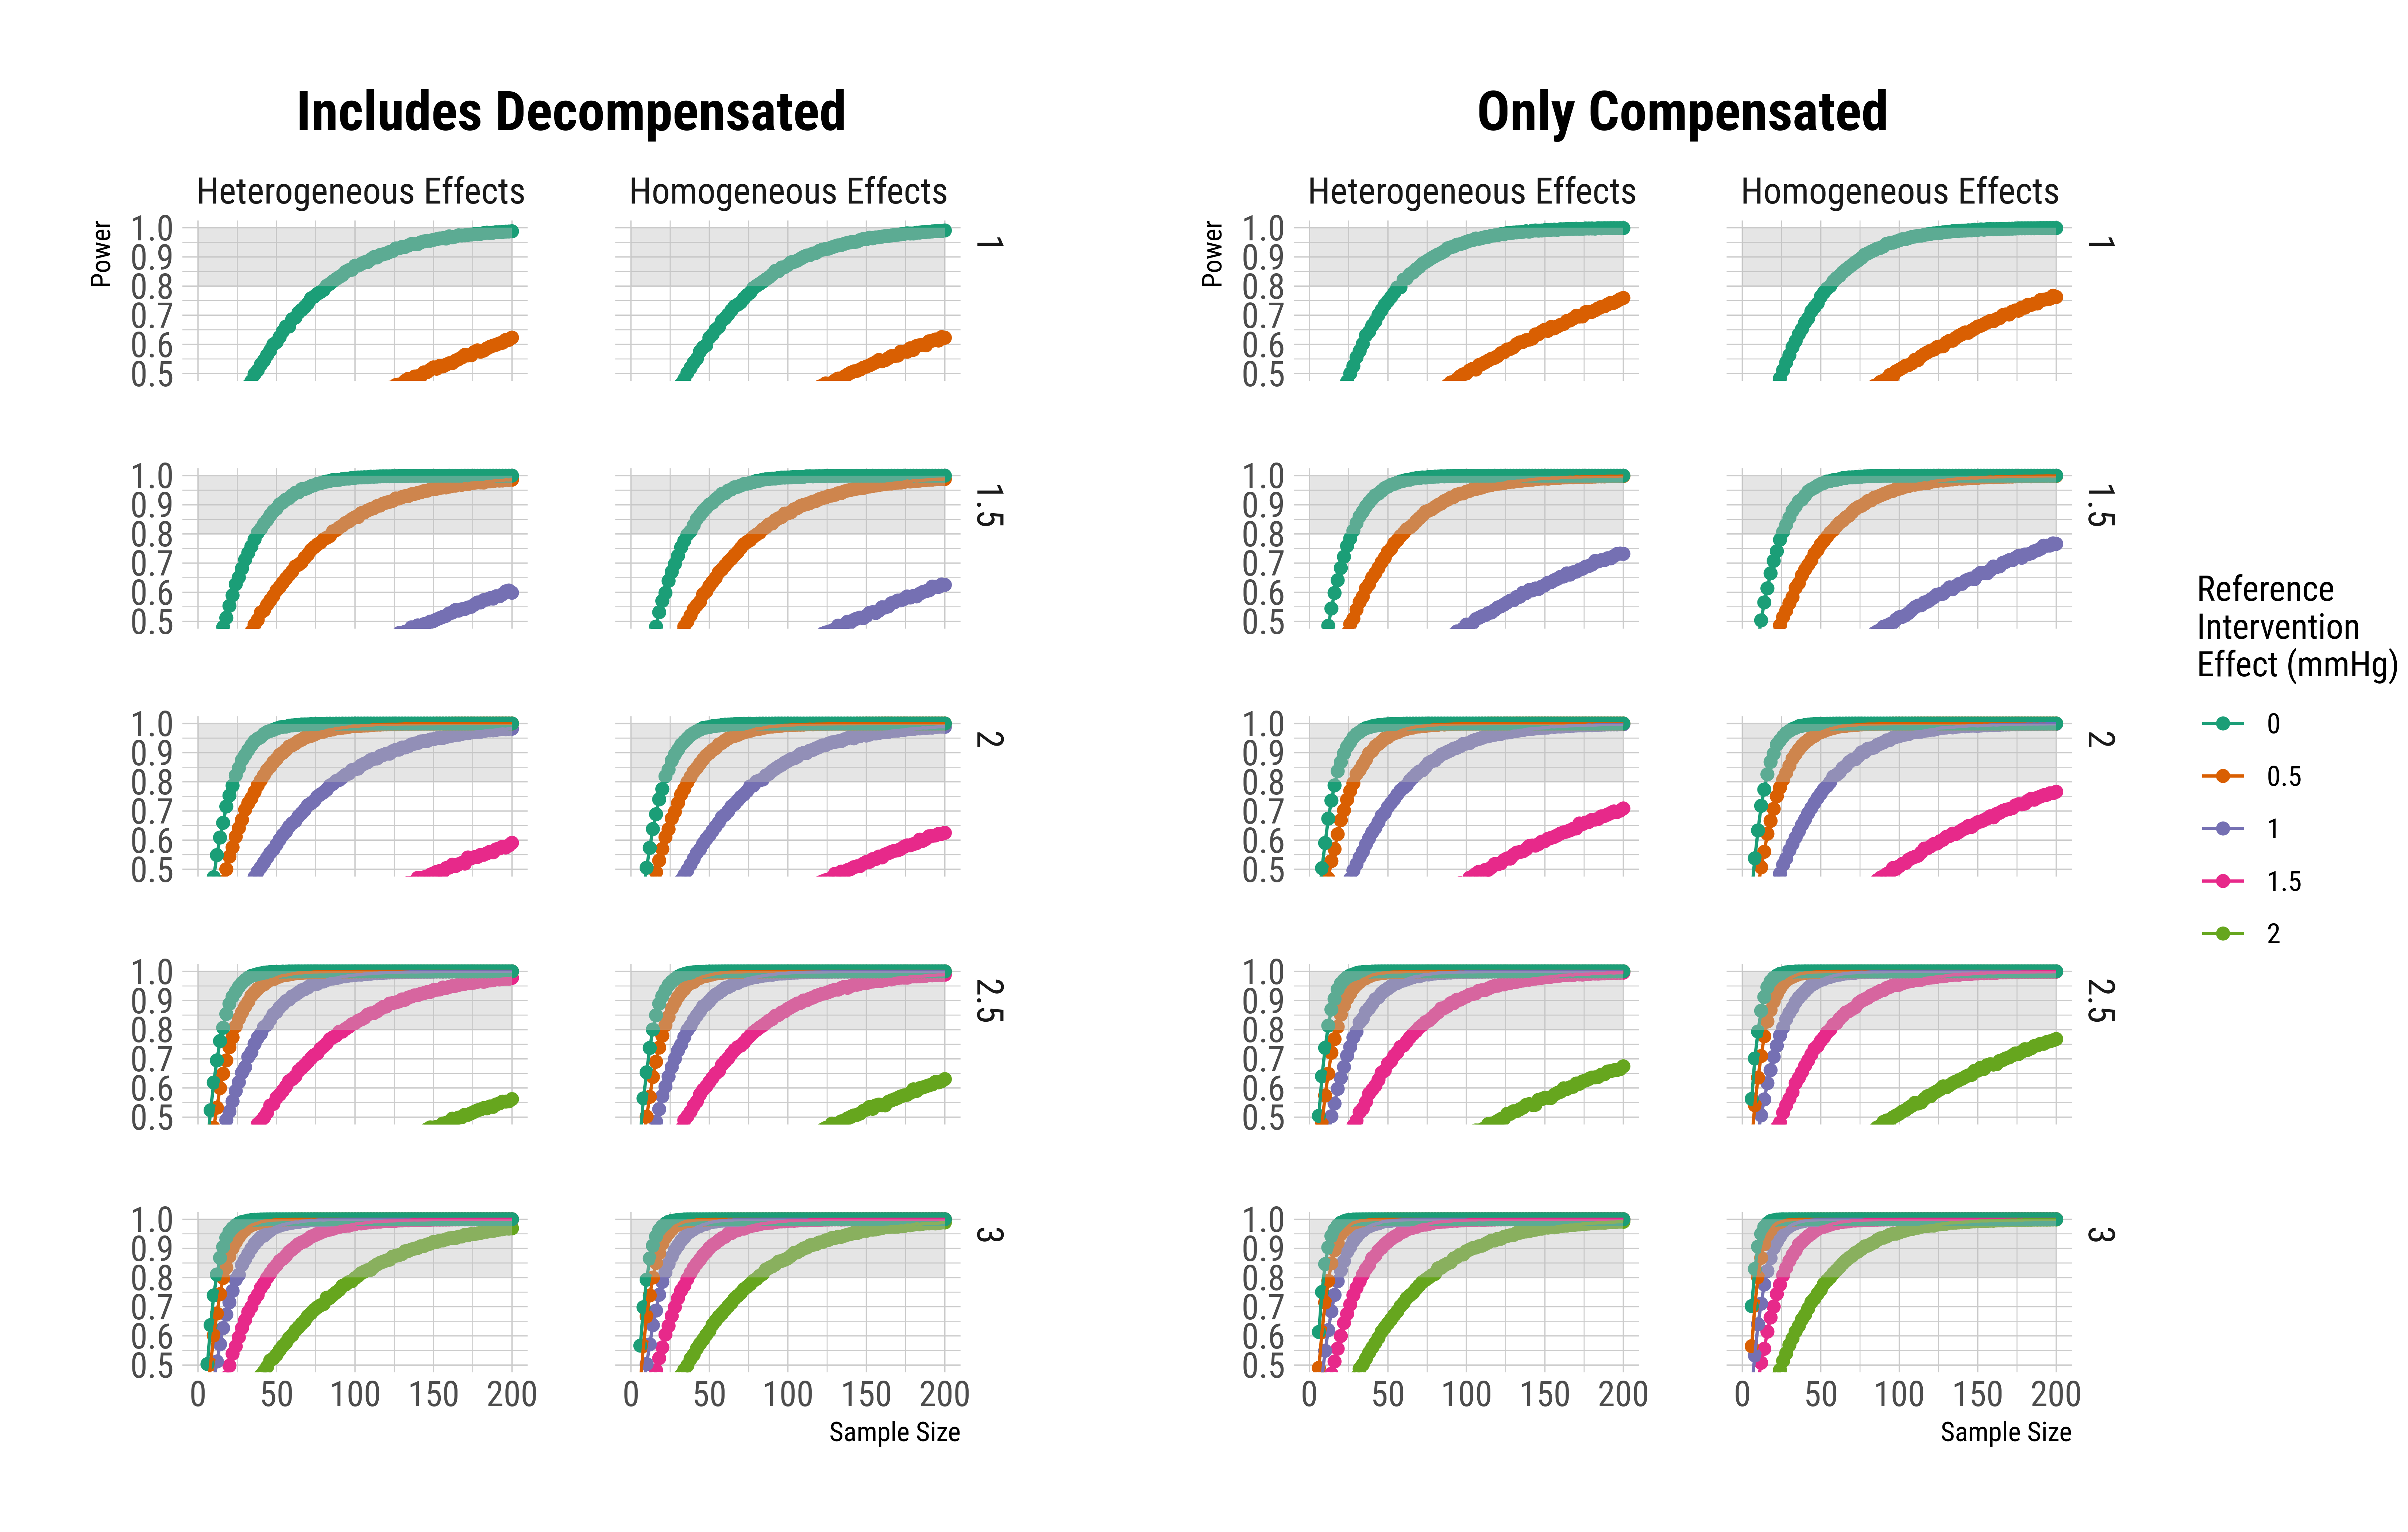
\includegraphics{figures/unnamed-chunk-76-1.png}

\hypertarget{required-individuals-1}{%
\subsection{Required Individuals}\label{required-individuals-1}}

And how many people do we need for each scenario?

\begin{Shaded}
\begin{Highlighting}[]
\NormalTok{difindifsims\_80power }\OtherTok{\textless{}{-}}\NormalTok{ difindifsims\_res }\SpecialCharTok{\%\textgreater{}\%} 
  \FunctionTok{arrange}\NormalTok{(power) }\SpecialCharTok{\%\textgreater{}\%} 
  \FunctionTok{filter}\NormalTok{(power }\SpecialCharTok{\textgreater{}} \FloatTok{0.8}\NormalTok{) }\SpecialCharTok{\%\textgreater{}\%} 
  \FunctionTok{select}\NormalTok{(decomp, deltadif, delta1, delta2, Effects, n) }\SpecialCharTok{\%\textgreater{}\%} 
  \FunctionTok{group\_by}\NormalTok{(delta1, deltadif, Effects, decomp) }\SpecialCharTok{\%\textgreater{}\%} 
  \FunctionTok{slice}\NormalTok{(}\DecValTok{1}\NormalTok{) }\SpecialCharTok{\%\textgreater{}\%} 
  \FunctionTok{arrange}\NormalTok{(decomp, }\FunctionTok{desc}\NormalTok{(deltadif), }\FunctionTok{desc}\NormalTok{(delta1), Effects) }\SpecialCharTok{\%\textgreater{}\%} 
  \FunctionTok{rename}\NormalTok{(}\StringTok{"Patients"} \OtherTok{=}\NormalTok{ decomp,}
         \StringTok{"Intervention 1 Effect (mmHg)"} \OtherTok{=}\NormalTok{ delta1,}
         \StringTok{"Intervention 2 Effect (mmHg)"} \OtherTok{=}\NormalTok{ delta2,}
         \StringTok{"Difference (mmHg)"} \OtherTok{=}\NormalTok{ deltadif,}
         \StringTok{"80\% Power"} \OtherTok{=}\NormalTok{ n)}

\NormalTok{difindifsims\_90power }\OtherTok{\textless{}{-}}\NormalTok{ difindifsims\_res }\SpecialCharTok{\%\textgreater{}\%} 
  \FunctionTok{arrange}\NormalTok{(power) }\SpecialCharTok{\%\textgreater{}\%} 
  \FunctionTok{filter}\NormalTok{(power }\SpecialCharTok{\textgreater{}} \FloatTok{0.9}\NormalTok{) }\SpecialCharTok{\%\textgreater{}\%} 
  \FunctionTok{select}\NormalTok{(decomp, deltadif, delta1, delta2, Effects, n) }\SpecialCharTok{\%\textgreater{}\%} 
  \FunctionTok{group\_by}\NormalTok{(delta1, deltadif, Effects, decomp) }\SpecialCharTok{\%\textgreater{}\%} 
  \FunctionTok{slice}\NormalTok{(}\DecValTok{1}\NormalTok{) }\SpecialCharTok{\%\textgreater{}\%} 
  \FunctionTok{arrange}\NormalTok{(decomp, }\FunctionTok{desc}\NormalTok{(deltadif), }\FunctionTok{desc}\NormalTok{(delta1), Effects) }\SpecialCharTok{\%\textgreater{}\%} 
  \FunctionTok{rename}\NormalTok{(}\StringTok{"Patients"} \OtherTok{=}\NormalTok{ decomp,}
         \StringTok{"Intervention 1 Effect (mmHg)"} \OtherTok{=}\NormalTok{ delta1,}
         \StringTok{"Intervention 2 Effect (mmHg)"} \OtherTok{=}\NormalTok{ delta2,}
         \StringTok{"Difference (mmHg)"} \OtherTok{=}\NormalTok{ deltadif,}
         \StringTok{"90\% Power"} \OtherTok{=}\NormalTok{ n)}

\NormalTok{difindifsims\_power }\OtherTok{\textless{}{-}} \FunctionTok{left\_join}\NormalTok{(difindifsims\_80power, difindifsims\_90power) }\SpecialCharTok{\%\textgreater{}\%}
  \FunctionTok{mutate}\NormalTok{(}\StringTok{\textasciigrave{}}\AttributeTok{90\% Power}\StringTok{\textasciigrave{}} \OtherTok{=} \FunctionTok{as.character}\NormalTok{(}\StringTok{\textasciigrave{}}\AttributeTok{90\% Power}\StringTok{\textasciigrave{}}\NormalTok{)) }\SpecialCharTok{\%\textgreater{}\%} 
  \FunctionTok{mutate}\NormalTok{(}\StringTok{\textasciigrave{}}\AttributeTok{90\% Power}\StringTok{\textasciigrave{}} \OtherTok{=} \FunctionTok{ifelse}\NormalTok{(}\FunctionTok{is.na}\NormalTok{(}\StringTok{\textasciigrave{}}\AttributeTok{90\% Power}\StringTok{\textasciigrave{}}\NormalTok{),}
                              \StringTok{"\textgreater{}200"}\NormalTok{, }\StringTok{\textasciigrave{}}\AttributeTok{90\% Power}\StringTok{\textasciigrave{}}\NormalTok{)) }\SpecialCharTok{\%\textgreater{}\%} 
  \FunctionTok{filter}\NormalTok{(}\StringTok{\textasciigrave{}}\AttributeTok{Difference (mmHg)}\StringTok{\textasciigrave{}} \SpecialCharTok{!=} \FloatTok{0.5}\NormalTok{)}

\NormalTok{decomp\_change }\OtherTok{\textless{}{-}} \FunctionTok{head}\NormalTok{(}
  \FunctionTok{which}\NormalTok{(}
\NormalTok{    difindifsims\_power}\SpecialCharTok{$}\NormalTok{Patients }\SpecialCharTok{==}
\NormalTok{      trt\_all}\SpecialCharTok{$}\NormalTok{decomp[}\DecValTok{2}\NormalTok{]), }\DecValTok{1}\NormalTok{)}

\FunctionTok{kable}\NormalTok{(difindifsims\_power[,}\SpecialCharTok{{-}}\DecValTok{1}\NormalTok{]) }\SpecialCharTok{\%\textgreater{}\%} 
  \FunctionTok{kable\_styling}\NormalTok{(}\StringTok{"striped"}\NormalTok{, }\AttributeTok{full\_width =}\NormalTok{ F) }\SpecialCharTok{\%\textgreater{}\%}
  \FunctionTok{pack\_rows}\NormalTok{(trt\_all}\SpecialCharTok{$}\NormalTok{decomp[}\DecValTok{1}\NormalTok{], }\DecValTok{1}\NormalTok{, decomp\_change}\DecValTok{{-}1}\NormalTok{) }\SpecialCharTok{\%\textgreater{}\%}
  \FunctionTok{pack\_rows}\NormalTok{(trt\_all}\SpecialCharTok{$}\NormalTok{decomp[}\DecValTok{2}\NormalTok{], decomp\_change, }\FunctionTok{nrow}\NormalTok{(difindifsims\_power))}
\end{Highlighting}
\end{Shaded}

\begin{table}[H]
\centering
\begin{tabular}{l|l|l|l|r|l}
\hline
Difference (mmHg) & Intervention 1 Effect (mmHg) & Intervention 2 Effect (mmHg) & Effects & 80\% Power & 90\% Power\\
\hline
\multicolumn{6}{l}{\textbf{Includes Decompensated}}\\
\hline
\hspace{1em}3 & 3 & 0 & Heterogeneous Effects & 12 & 16\\
\hline
\hspace{1em}3 & 3 & 0 & Homogeneous Effects & 12 & 14\\
\hline
\hspace{1em}2.5 & 3 & 0.5 & Heterogeneous Effects & 18 & 22\\
\hline
\hspace{1em}2.5 & 3 & 0.5 & Homogeneous Effects & 16 & 20\\
\hline
\hspace{1em}2.5 & 2.5 & 0 & Heterogeneous Effects & 16 & 22\\
\hline
\hspace{1em}2.5 & 2.5 & 0 & Homogeneous Effects & 14 & 20\\
\hline
\hspace{1em}2 & 3 & 1 & Heterogeneous Effects & 26 & 36\\
\hline
\hspace{1em}2 & 3 & 1 & Homogeneous Effects & 22 & 30\\
\hline
\hspace{1em}2 & 2.5 & 0.5 & Heterogeneous Effects & 24 & 34\\
\hline
\hspace{1em}2 & 2.5 & 0.5 & Homogeneous Effects & 22 & 30\\
\hline
\hspace{1em}2 & 2 & 0 & Heterogeneous Effects & 24 & 32\\
\hline
\hspace{1em}2 & 2 & 0 & Homogeneous Effects & 22 & 30\\
\hline
\hspace{1em}1.5 & 3 & 1.5 & Heterogeneous Effects & 46 & 62\\
\hline
\hspace{1em}1.5 & 3 & 1.5 & Homogeneous Effects & 38 & 50\\
\hline
\hspace{1em}1.5 & 2.5 & 1 & Heterogeneous Effects & 42 & 58\\
\hline
\hspace{1em}1.5 & 2.5 & 1 & Homogeneous Effects & 38 & 52\\
\hline
\hspace{1em}1.5 & 2 & 0.5 & Heterogeneous Effects & 40 & 56\\
\hline
\hspace{1em}1.5 & 2 & 0.5 & Homogeneous Effects & 38 & 52\\
\hline
\hspace{1em}1.5 & 1.5 & 0 & Heterogeneous Effects & 38 & 52\\
\hline
\hspace{1em}1.5 & 1.5 & 0 & Homogeneous Effects & 38 & 50\\
\hline
\hspace{1em}1 & 3 & 2 & Heterogeneous Effects & 102 & 140\\
\hline
\hspace{1em}1 & 3 & 2 & Homogeneous Effects & 82 & 112\\
\hline
\hspace{1em}1 & 2.5 & 1.5 & Heterogeneous Effects & 94 & 132\\
\hline
\hspace{1em}1 & 2.5 & 1.5 & Homogeneous Effects & 82 & 110\\
\hline
\hspace{1em}1 & 2 & 1 & Heterogeneous Effects & 88 & 124\\
\hline
\hspace{1em}1 & 2 & 1 & Homogeneous Effects & 80 & 114\\
\hline
\hspace{1em}1 & 1.5 & 0.5 & Heterogeneous Effects & 86 & 118\\
\hline
\hspace{1em}1 & 1.5 & 0.5 & Homogeneous Effects & 82 & 112\\
\hline
\hspace{1em}1 & 1 & 0 & Heterogeneous Effects & 82 & 116\\
\hline
\hspace{1em}1 & 1 & 0 & Homogeneous Effects & 80 & 112\\
\hline
\multicolumn{6}{l}{\textbf{Only Compensated}}\\
\hline
\hspace{1em}3 & 3 & 0 & Heterogeneous Effects & 10 & 12\\
\hline
\hspace{1em}3 & 3 & 0 & Homogeneous Effects & 8 & 10\\
\hline
\hspace{1em}2.5 & 3 & 0.5 & Heterogeneous Effects & 14 & 18\\
\hline
\hspace{1em}2.5 & 3 & 0.5 & Homogeneous Effects & 10 & 14\\
\hline
\hspace{1em}2.5 & 2.5 & 0 & Heterogeneous Effects & 12 & 16\\
\hline
\hspace{1em}2.5 & 2.5 & 0 & Homogeneous Effects & 12 & 14\\
\hline
\hspace{1em}2 & 3 & 1 & Heterogeneous Effects & 20 & 26\\
\hline
\hspace{1em}2 & 3 & 1 & Homogeneous Effects & 16 & 20\\
\hline
\hspace{1em}2 & 2.5 & 0.5 & Heterogeneous Effects & 18 & 24\\
\hline
\hspace{1em}2 & 2.5 & 0.5 & Homogeneous Effects & 16 & 22\\
\hline
\hspace{1em}2 & 2 & 0 & Heterogeneous Effects & 18 & 24\\
\hline
\hspace{1em}2 & 2 & 0 & Homogeneous Effects & 16 & 22\\
\hline
\hspace{1em}1.5 & 3 & 1.5 & Heterogeneous Effects & 34 & 46\\
\hline
\hspace{1em}1.5 & 3 & 1.5 & Homogeneous Effects & 26 & 36\\
\hline
\hspace{1em}1.5 & 2.5 & 1 & Heterogeneous Effects & 32 & 42\\
\hline
\hspace{1em}1.5 & 2.5 & 1 & Homogeneous Effects & 26 & 36\\
\hline
\hspace{1em}1.5 & 2 & 0.5 & Heterogeneous Effects & 30 & 40\\
\hline
\hspace{1em}1.5 & 2 & 0.5 & Homogeneous Effects & 26 & 36\\
\hline
\hspace{1em}1.5 & 1.5 & 0 & Heterogeneous Effects & 28 & 38\\
\hline
\hspace{1em}1.5 & 1.5 & 0 & Homogeneous Effects & 26 & 36\\
\hline
\hspace{1em}1 & 3 & 2 & Heterogeneous Effects & 76 & 104\\
\hline
\hspace{1em}1 & 3 & 2 & Homogeneous Effects & 56 & 78\\
\hline
\hspace{1em}1 & 2.5 & 1.5 & Heterogeneous Effects & 70 & 94\\
\hline
\hspace{1em}1 & 2.5 & 1.5 & Homogeneous Effects & 56 & 78\\
\hline
\hspace{1em}1 & 2 & 1 & Heterogeneous Effects & 64 & 88\\
\hline
\hspace{1em}1 & 2 & 1 & Homogeneous Effects & 58 & 76\\
\hline
\hspace{1em}1 & 1.5 & 0.5 & Heterogeneous Effects & 60 & 84\\
\hline
\hspace{1em}1 & 1.5 & 0.5 & Homogeneous Effects & 56 & 78\\
\hline
\hspace{1em}1 & 1 & 0 & Heterogeneous Effects & 60 & 80\\
\hline
\hspace{1em}1 & 1 & 0 & Homogeneous Effects & 58 & 78\\
\hline
\end{tabular}
\end{table}

\begin{Shaded}
\begin{Highlighting}[]
\NormalTok{difindiftable\_decomp }\OtherTok{\textless{}{-}}\NormalTok{ difindifsims\_power }\SpecialCharTok{\%\textgreater{}\%} 
  \FunctionTok{filter}\NormalTok{(Patients}\SpecialCharTok{==}\StringTok{"Includes Decompensated"}\NormalTok{) }\SpecialCharTok{\%\textgreater{}\%} 
  \FunctionTok{ungroup}\NormalTok{() }\SpecialCharTok{\%\textgreater{}\%} 
  \FunctionTok{select}\NormalTok{(}\SpecialCharTok{{-}}\NormalTok{Patients) }\SpecialCharTok{\%\textgreater{}\%} 
  \FunctionTok{kable}\NormalTok{() }\SpecialCharTok{\%\textgreater{}\%} 
  \FunctionTok{kable\_styling}\NormalTok{(}\StringTok{"striped"}\NormalTok{, }\AttributeTok{full\_width =}\NormalTok{ F) }\SpecialCharTok{\%\textgreater{}\%}
  \FunctionTok{pack\_rows}\NormalTok{(}\StringTok{"Includes Decompensated"}\NormalTok{, }\DecValTok{1}\NormalTok{, decomp\_change}\DecValTok{{-}1}\NormalTok{) }

\NormalTok{difindiftable\_comp }\OtherTok{\textless{}{-}}\NormalTok{ difindifsims\_power }\SpecialCharTok{\%\textgreater{}\%} 
  \FunctionTok{filter}\NormalTok{(Patients}\SpecialCharTok{==}\StringTok{"Only Compensated"}\NormalTok{) }\SpecialCharTok{\%\textgreater{}\%} 
  \FunctionTok{ungroup}\NormalTok{() }\SpecialCharTok{\%\textgreater{}\%} 
  \FunctionTok{select}\NormalTok{(}\SpecialCharTok{{-}}\NormalTok{Patients) }\SpecialCharTok{\%\textgreater{}\%} 
  \FunctionTok{kable}\NormalTok{() }\SpecialCharTok{\%\textgreater{}\%} 
  \FunctionTok{kable\_styling}\NormalTok{(}\StringTok{"striped"}\NormalTok{, }\AttributeTok{full\_width =}\NormalTok{ F) }\SpecialCharTok{\%\textgreater{}\%}
  \FunctionTok{pack\_rows}\NormalTok{(}\StringTok{"Only Compensated"}\NormalTok{, }\DecValTok{1}\NormalTok{, decomp\_change}\DecValTok{{-}1}\NormalTok{)}

\NormalTok{difindiftable\_decomp}
\end{Highlighting}
\end{Shaded}

\begin{table}[H]
\centering
\begin{tabular}{l|l|l|l|r|l}
\hline
Difference (mmHg) & Intervention 1 Effect (mmHg) & Intervention 2 Effect (mmHg) & Effects & 80\% Power & 90\% Power\\
\hline
\multicolumn{6}{l}{\textbf{Includes Decompensated}}\\
\hline
\hspace{1em}3 & 3 & 0 & Heterogeneous Effects & 12 & 16\\
\hline
\hspace{1em}3 & 3 & 0 & Homogeneous Effects & 12 & 14\\
\hline
\hspace{1em}2.5 & 3 & 0.5 & Heterogeneous Effects & 18 & 22\\
\hline
\hspace{1em}2.5 & 3 & 0.5 & Homogeneous Effects & 16 & 20\\
\hline
\hspace{1em}2.5 & 2.5 & 0 & Heterogeneous Effects & 16 & 22\\
\hline
\hspace{1em}2.5 & 2.5 & 0 & Homogeneous Effects & 14 & 20\\
\hline
\hspace{1em}2 & 3 & 1 & Heterogeneous Effects & 26 & 36\\
\hline
\hspace{1em}2 & 3 & 1 & Homogeneous Effects & 22 & 30\\
\hline
\hspace{1em}2 & 2.5 & 0.5 & Heterogeneous Effects & 24 & 34\\
\hline
\hspace{1em}2 & 2.5 & 0.5 & Homogeneous Effects & 22 & 30\\
\hline
\hspace{1em}2 & 2 & 0 & Heterogeneous Effects & 24 & 32\\
\hline
\hspace{1em}2 & 2 & 0 & Homogeneous Effects & 22 & 30\\
\hline
\hspace{1em}1.5 & 3 & 1.5 & Heterogeneous Effects & 46 & 62\\
\hline
\hspace{1em}1.5 & 3 & 1.5 & Homogeneous Effects & 38 & 50\\
\hline
\hspace{1em}1.5 & 2.5 & 1 & Heterogeneous Effects & 42 & 58\\
\hline
\hspace{1em}1.5 & 2.5 & 1 & Homogeneous Effects & 38 & 52\\
\hline
\hspace{1em}1.5 & 2 & 0.5 & Heterogeneous Effects & 40 & 56\\
\hline
\hspace{1em}1.5 & 2 & 0.5 & Homogeneous Effects & 38 & 52\\
\hline
\hspace{1em}1.5 & 1.5 & 0 & Heterogeneous Effects & 38 & 52\\
\hline
\hspace{1em}1.5 & 1.5 & 0 & Homogeneous Effects & 38 & 50\\
\hline
\hspace{1em}1 & 3 & 2 & Heterogeneous Effects & 102 & 140\\
\hline
\hspace{1em}1 & 3 & 2 & Homogeneous Effects & 82 & 112\\
\hline
\hspace{1em}1 & 2.5 & 1.5 & Heterogeneous Effects & 94 & 132\\
\hline
\hspace{1em}1 & 2.5 & 1.5 & Homogeneous Effects & 82 & 110\\
\hline
\hspace{1em}1 & 2 & 1 & Heterogeneous Effects & 88 & 124\\
\hline
\hspace{1em}1 & 2 & 1 & Homogeneous Effects & 80 & 114\\
\hline
\hspace{1em}1 & 1.5 & 0.5 & Heterogeneous Effects & 86 & 118\\
\hline
\hspace{1em}1 & 1.5 & 0.5 & Homogeneous Effects & 82 & 112\\
\hline
\hspace{1em}1 & 1 & 0 & Heterogeneous Effects & 82 & 116\\
\hline
\hspace{1em}1 & 1 & 0 & Homogeneous Effects & 80 & 112\\
\hline
\end{tabular}
\end{table}

\begin{Shaded}
\begin{Highlighting}[]
\NormalTok{difindiftable\_comp}
\end{Highlighting}
\end{Shaded}

\begin{table}[H]
\centering
\begin{tabular}{l|l|l|l|r|l}
\hline
Difference (mmHg) & Intervention 1 Effect (mmHg) & Intervention 2 Effect (mmHg) & Effects & 80\% Power & 90\% Power\\
\hline
\multicolumn{6}{l}{\textbf{Only Compensated}}\\
\hline
\hspace{1em}3 & 3 & 0 & Heterogeneous Effects & 10 & 12\\
\hline
\hspace{1em}3 & 3 & 0 & Homogeneous Effects & 8 & 10\\
\hline
\hspace{1em}2.5 & 3 & 0.5 & Heterogeneous Effects & 14 & 18\\
\hline
\hspace{1em}2.5 & 3 & 0.5 & Homogeneous Effects & 10 & 14\\
\hline
\hspace{1em}2.5 & 2.5 & 0 & Heterogeneous Effects & 12 & 16\\
\hline
\hspace{1em}2.5 & 2.5 & 0 & Homogeneous Effects & 12 & 14\\
\hline
\hspace{1em}2 & 3 & 1 & Heterogeneous Effects & 20 & 26\\
\hline
\hspace{1em}2 & 3 & 1 & Homogeneous Effects & 16 & 20\\
\hline
\hspace{1em}2 & 2.5 & 0.5 & Heterogeneous Effects & 18 & 24\\
\hline
\hspace{1em}2 & 2.5 & 0.5 & Homogeneous Effects & 16 & 22\\
\hline
\hspace{1em}2 & 2 & 0 & Heterogeneous Effects & 18 & 24\\
\hline
\hspace{1em}2 & 2 & 0 & Homogeneous Effects & 16 & 22\\
\hline
\hspace{1em}1.5 & 3 & 1.5 & Heterogeneous Effects & 34 & 46\\
\hline
\hspace{1em}1.5 & 3 & 1.5 & Homogeneous Effects & 26 & 36\\
\hline
\hspace{1em}1.5 & 2.5 & 1 & Heterogeneous Effects & 32 & 42\\
\hline
\hspace{1em}1.5 & 2.5 & 1 & Homogeneous Effects & 26 & 36\\
\hline
\hspace{1em}1.5 & 2 & 0.5 & Heterogeneous Effects & 30 & 40\\
\hline
\hspace{1em}1.5 & 2 & 0.5 & Homogeneous Effects & 26 & 36\\
\hline
\hspace{1em}1.5 & 1.5 & 0 & Heterogeneous Effects & 28 & 38\\
\hline
\hspace{1em}1.5 & 1.5 & 0 & Homogeneous Effects & 26 & 36\\
\hline
\hspace{1em}1 & 3 & 2 & Heterogeneous Effects & 76 & 104\\
\hline
\hspace{1em}1 & 3 & 2 & Homogeneous Effects & 56 & 78\\
\hline
\hspace{1em}1 & 2.5 & 1.5 & Heterogeneous Effects & 70 & 94\\
\hline
\hspace{1em}1 & 2.5 & 1.5 & Homogeneous Effects & 56 & 78\\
\hline
\hspace{1em}1 & 2 & 1 & Heterogeneous Effects & 64 & 88\\
\hline
\hspace{1em}1 & 2 & 1 & Homogeneous Effects & 58 & 76\\
\hline
\hspace{1em}1 & 1.5 & 0.5 & Heterogeneous Effects & 60 & 84\\
\hline
\hspace{1em}1 & 1.5 & 0.5 & Homogeneous Effects & 56 & 78\\
\hline
\hspace{1em}1 & 1 & 0 & Heterogeneous Effects & 60 & 80\\
\hline
\hspace{1em}1 & 1 & 0 & Homogeneous Effects & 58 & 78\\
\hline
\end{tabular}
\end{table}

\begin{Shaded}
\begin{Highlighting}[]
\CommentTok{\# save\_kable(difindiftable\_decomp, "figures/difindifpower\_dc.jpg")}
\CommentTok{\# save\_kable(difindiftable\_comp, "figures/difindifpower\_c.jpg")}
\end{Highlighting}
\end{Shaded}

\hypertarget{contour-plot}{%
\subsection{Contour Plot}\label{contour-plot}}

First let's look at different deltadif values.

\begin{Shaded}
\begin{Highlighting}[]
\NormalTok{difindifsims\_res\_hom }\OtherTok{\textless{}{-}}\NormalTok{ difindifsims\_res }\SpecialCharTok{\%\textgreater{}\%} 
  \FunctionTok{filter}\NormalTok{(cv\_delta}\SpecialCharTok{==}\DecValTok{0}\NormalTok{) }\SpecialCharTok{\%\textgreater{}\%} 
  \FunctionTok{mutate}\NormalTok{(}\AttributeTok{delta1 =} \FunctionTok{as.numeric}\NormalTok{(}\FunctionTok{as.character}\NormalTok{(delta1)),}
         \AttributeTok{delta2 =} \FunctionTok{as.numeric}\NormalTok{(}\FunctionTok{as.character}\NormalTok{(delta2)),}
         \AttributeTok{deltadif =} \FunctionTok{as.numeric}\NormalTok{(}\FunctionTok{as.character}\NormalTok{(deltadif))) }\SpecialCharTok{\%\textgreater{}\%} 
  \FunctionTok{mutate}\NormalTok{(}\AttributeTok{power =} \FunctionTok{ifelse}\NormalTok{(power }\SpecialCharTok{==} \DecValTok{1}\NormalTok{, }\FloatTok{0.99}\NormalTok{, power)) }

\NormalTok{difindifsims\_res\_het }\OtherTok{\textless{}{-}}\NormalTok{ difindifsims\_res }\SpecialCharTok{\%\textgreater{}\%} 
  \FunctionTok{filter}\NormalTok{(cv\_delta}\SpecialCharTok{!=}\DecValTok{0}\NormalTok{) }\SpecialCharTok{\%\textgreater{}\%} 
  \FunctionTok{mutate}\NormalTok{(}\AttributeTok{delta1 =} \FunctionTok{as.numeric}\NormalTok{(}\FunctionTok{as.character}\NormalTok{(delta1)),}
         \AttributeTok{delta2 =} \FunctionTok{as.numeric}\NormalTok{(}\FunctionTok{as.character}\NormalTok{(delta2)),}
         \AttributeTok{deltadif =} \FunctionTok{as.numeric}\NormalTok{(}\FunctionTok{as.character}\NormalTok{(deltadif))) }\SpecialCharTok{\%\textgreater{}\%} 
  \FunctionTok{mutate}\NormalTok{(}\AttributeTok{power =} \FunctionTok{ifelse}\NormalTok{(power }\SpecialCharTok{==} \DecValTok{1}\NormalTok{, }\FloatTok{0.99}\NormalTok{, power)) }

\NormalTok{difindif\_cont1\_hom }\OtherTok{\textless{}{-}}\NormalTok{ difindifsims\_res\_hom }\SpecialCharTok{\%\textgreater{}\%} 
  \FunctionTok{filter}\NormalTok{(deltadif}\SpecialCharTok{!=}\DecValTok{3}\NormalTok{) }\SpecialCharTok{\%\textgreater{}\%} 
  \FunctionTok{ggplot}\NormalTok{(}\FunctionTok{aes}\NormalTok{(}\AttributeTok{x=}\NormalTok{n, }\AttributeTok{y=}\NormalTok{delta1, }\AttributeTok{z=}\NormalTok{power)) }\SpecialCharTok{+}
  \FunctionTok{geom\_contour\_filled}\NormalTok{(}\AttributeTok{alpha=}\FloatTok{0.8}\NormalTok{, }\AttributeTok{breaks=}\FunctionTok{seq}\NormalTok{(}\DecValTok{0}\NormalTok{,}\FloatTok{1.1}\NormalTok{, }\AttributeTok{by=}\FloatTok{0.1}\NormalTok{)) }\SpecialCharTok{+}
  \FunctionTok{facet\_grid}\NormalTok{(deltadif}\SpecialCharTok{\textasciitilde{}}\NormalTok{decomp, }\AttributeTok{scales =} \StringTok{"free"}\NormalTok{) }\SpecialCharTok{+}
  \FunctionTok{theme\_ipsum\_rc}\NormalTok{() }\SpecialCharTok{+}
  \FunctionTok{labs}\NormalTok{(}\AttributeTok{x =} \StringTok{"Sample Size"}\NormalTok{,}
       \AttributeTok{y =} \StringTok{"Hypothetical Intervention Effect of Main Treatment (mmHg)"}\NormalTok{,}
       \AttributeTok{subtitle =} \StringTok{"Comparison of Differences of Effects between Interventions"}\NormalTok{) }\SpecialCharTok{+}
  \FunctionTok{scale\_y\_continuous}\NormalTok{(}\AttributeTok{breaks =} \FunctionTok{seq}\NormalTok{(}\FloatTok{0.5}\NormalTok{, }\DecValTok{5}\NormalTok{, }\AttributeTok{by =} \FloatTok{0.5}\NormalTok{)) }\SpecialCharTok{+}
  \FunctionTok{scale\_fill\_viridis}\NormalTok{(}\StringTok{"Power"}\NormalTok{, }\AttributeTok{discrete =}\NormalTok{ T) }\SpecialCharTok{+}
  \FunctionTok{geom\_contour}\NormalTok{(}\AttributeTok{breaks=}\FloatTok{0.8}\NormalTok{, }\AttributeTok{colour=}\StringTok{"black"}\NormalTok{, }\AttributeTok{linetype=}\StringTok{"dashed"}\NormalTok{)}

\NormalTok{difindif\_cont1\_hom}
\end{Highlighting}
\end{Shaded}

\includegraphics{figures/unnamed-chunk-78-1.png}

\begin{Shaded}
\begin{Highlighting}[]
\NormalTok{difindif\_cont1\_het }\OtherTok{\textless{}{-}}\NormalTok{ difindifsims\_res\_het }\SpecialCharTok{\%\textgreater{}\%} 
  \FunctionTok{filter}\NormalTok{(deltadif}\SpecialCharTok{!=}\DecValTok{3}\NormalTok{) }\SpecialCharTok{\%\textgreater{}\%} 
  \FunctionTok{ggplot}\NormalTok{(}\FunctionTok{aes}\NormalTok{(}\AttributeTok{x=}\NormalTok{n, }\AttributeTok{y=}\NormalTok{delta1, }\AttributeTok{z=}\NormalTok{power)) }\SpecialCharTok{+}
  \FunctionTok{geom\_contour\_filled}\NormalTok{(}\AttributeTok{alpha=}\FloatTok{0.8}\NormalTok{, }\AttributeTok{breaks=}\FunctionTok{seq}\NormalTok{(}\DecValTok{0}\NormalTok{,}\FloatTok{1.1}\NormalTok{, }\AttributeTok{by=}\FloatTok{0.1}\NormalTok{)) }\SpecialCharTok{+}
  \FunctionTok{facet\_grid}\NormalTok{(deltadif}\SpecialCharTok{\textasciitilde{}}\NormalTok{decomp, }\AttributeTok{scales =} \StringTok{"free"}\NormalTok{) }\SpecialCharTok{+}
  \FunctionTok{theme\_ipsum\_rc}\NormalTok{() }\SpecialCharTok{+}
  \FunctionTok{labs}\NormalTok{(}\AttributeTok{x =} \StringTok{"Sample Size"}\NormalTok{,}
       \AttributeTok{y =} \StringTok{"Hypothetical Intervention Effect of Main Treatment (mmHg)"}\NormalTok{,}
       \AttributeTok{subtitle =} \StringTok{"Comparison of Differences of Effects between Interventions"}\NormalTok{) }\SpecialCharTok{+}
  \FunctionTok{scale\_y\_continuous}\NormalTok{(}\AttributeTok{breaks =} \FunctionTok{seq}\NormalTok{(}\FloatTok{0.5}\NormalTok{, }\DecValTok{5}\NormalTok{, }\AttributeTok{by =} \FloatTok{0.5}\NormalTok{)) }\SpecialCharTok{+}
  \FunctionTok{scale\_fill\_viridis}\NormalTok{(}\StringTok{"Power"}\NormalTok{, }\AttributeTok{discrete =}\NormalTok{ T) }\SpecialCharTok{+}
  \FunctionTok{geom\_contour}\NormalTok{(}\AttributeTok{breaks=}\FloatTok{0.8}\NormalTok{, }\AttributeTok{colour=}\StringTok{"black"}\NormalTok{, }\AttributeTok{linetype=}\StringTok{"dashed"}\NormalTok{)    }

\NormalTok{difindif\_cont1\_het}
\end{Highlighting}
\end{Shaded}

\includegraphics{figures/unnamed-chunk-78-2.png} This is helpful to
visualise, though probably not for the paper. With homogeneous effects,
the determinant of the power is the difference in intervention effects;
it's a straight line. With heterogeneous effects, the line is not
straight

\begin{Shaded}
\begin{Highlighting}[]
\NormalTok{difindif\_cont2\_hom }\OtherTok{\textless{}{-}} \FunctionTok{ggplot}\NormalTok{(difindifsims\_res\_hom, }\FunctionTok{aes}\NormalTok{(}\AttributeTok{x=}\NormalTok{n, }\AttributeTok{y=}\NormalTok{delta1, }\AttributeTok{z=}\NormalTok{power)) }\SpecialCharTok{+}
  \FunctionTok{geom\_contour\_filled}\NormalTok{(}\AttributeTok{alpha=}\FloatTok{0.8}\NormalTok{, }\AttributeTok{breaks=}\FunctionTok{seq}\NormalTok{(}\DecValTok{0}\NormalTok{,}\FloatTok{1.1}\NormalTok{, }\AttributeTok{by=}\FloatTok{0.1}\NormalTok{)) }\SpecialCharTok{+}
  \FunctionTok{facet\_grid}\NormalTok{(delta2}\SpecialCharTok{\textasciitilde{}}\NormalTok{decomp, }\AttributeTok{scales =} \StringTok{"free"}\NormalTok{) }\SpecialCharTok{+}
  \FunctionTok{theme\_ipsum\_rc}\NormalTok{() }\SpecialCharTok{+}
  \FunctionTok{labs}\NormalTok{(}\AttributeTok{x =} \StringTok{"Sample Size"}\NormalTok{,}
       \AttributeTok{y =} \StringTok{"Hypothetical Intervention Effect of Main Treatment (mmHg)"}\NormalTok{,}
       \AttributeTok{subtitle =} \StringTok{"Comparisons Grouped by Intervention Effects of the Reference Treatment (mmHg)"}\NormalTok{) }\SpecialCharTok{+}
  \FunctionTok{scale\_y\_continuous}\NormalTok{(}\AttributeTok{breaks =} \FunctionTok{seq}\NormalTok{(}\FloatTok{0.5}\NormalTok{, }\DecValTok{5}\NormalTok{, }\AttributeTok{by =} \FloatTok{0.5}\NormalTok{)) }\SpecialCharTok{+}
  \FunctionTok{scale\_fill\_viridis}\NormalTok{(}\StringTok{"Power"}\NormalTok{, }\AttributeTok{discrete =}\NormalTok{ T) }\SpecialCharTok{+}
  \FunctionTok{geom\_contour}\NormalTok{(}\AttributeTok{breaks=}\FloatTok{0.8}\NormalTok{, }\AttributeTok{colour=}\StringTok{"black"}\NormalTok{, }\AttributeTok{linetype=}\StringTok{"dashed"}\NormalTok{)}

\NormalTok{difindif\_cont2\_hom}
\end{Highlighting}
\end{Shaded}

\includegraphics{figures/unnamed-chunk-79-1.png}

\begin{Shaded}
\begin{Highlighting}[]
\NormalTok{difindif\_cont2\_het }\OtherTok{\textless{}{-}} \FunctionTok{ggplot}\NormalTok{(difindifsims\_res\_het, }\FunctionTok{aes}\NormalTok{(}\AttributeTok{x=}\NormalTok{n, }\AttributeTok{y=}\NormalTok{delta1, }\AttributeTok{z=}\NormalTok{power)) }\SpecialCharTok{+}
  \FunctionTok{geom\_contour\_filled}\NormalTok{(}\AttributeTok{alpha=}\FloatTok{0.8}\NormalTok{, }\AttributeTok{breaks=}\FunctionTok{seq}\NormalTok{(}\DecValTok{0}\NormalTok{,}\FloatTok{1.1}\NormalTok{, }\AttributeTok{by=}\FloatTok{0.1}\NormalTok{)) }\SpecialCharTok{+}
  \FunctionTok{facet\_grid}\NormalTok{(delta2}\SpecialCharTok{\textasciitilde{}}\NormalTok{decomp, }\AttributeTok{scales =} \StringTok{"free"}\NormalTok{) }\SpecialCharTok{+}
  \FunctionTok{theme\_ipsum\_rc}\NormalTok{() }\SpecialCharTok{+}
  \FunctionTok{labs}\NormalTok{(}\AttributeTok{x =} \StringTok{"Sample Size"}\NormalTok{,}
       \AttributeTok{y =} \StringTok{"Hypothetical Intervention Effect of Main Treatment (mmHg)"}\NormalTok{,}
       \AttributeTok{subtitle =} \StringTok{"Comparisons Grouped by Intervention Effects of the Reference Treatment (mmHg)"}\NormalTok{) }\SpecialCharTok{+}
  \FunctionTok{scale\_y\_continuous}\NormalTok{(}\AttributeTok{breaks =} \FunctionTok{seq}\NormalTok{(}\FloatTok{0.5}\NormalTok{, }\DecValTok{5}\NormalTok{, }\AttributeTok{by =} \FloatTok{0.5}\NormalTok{)) }\SpecialCharTok{+}
  \FunctionTok{scale\_fill\_viridis}\NormalTok{(}\StringTok{"Power"}\NormalTok{, }\AttributeTok{discrete =}\NormalTok{ T) }\SpecialCharTok{+}
  \FunctionTok{geom\_contour}\NormalTok{(}\AttributeTok{breaks=}\FloatTok{0.8}\NormalTok{, }\AttributeTok{colour=}\StringTok{"black"}\NormalTok{, }\AttributeTok{linetype=}\StringTok{"dashed"}\NormalTok{)    }

\NormalTok{difindif\_cont2\_het}
\end{Highlighting}
\end{Shaded}

\includegraphics{figures/unnamed-chunk-79-2.png}

And just looking against placebo (i.e.~delta2=0)

\begin{Shaded}
\begin{Highlighting}[]
\NormalTok{difindif\_cont3\_hom }\OtherTok{\textless{}{-}}\NormalTok{ difindifsims\_res\_hom }\SpecialCharTok{\%\textgreater{}\%} 
  \FunctionTok{filter}\NormalTok{(deltadif}\SpecialCharTok{!=}\DecValTok{3}\NormalTok{) }\SpecialCharTok{\%\textgreater{}\%} 
  \FunctionTok{filter}\NormalTok{(delta2}\SpecialCharTok{==}\DecValTok{0}\NormalTok{) }\SpecialCharTok{\%\textgreater{}\%} 
  \FunctionTok{ggplot}\NormalTok{(}\FunctionTok{aes}\NormalTok{(}\AttributeTok{x=}\NormalTok{n, }\AttributeTok{y=}\NormalTok{delta1, }\AttributeTok{z=}\NormalTok{power)) }\SpecialCharTok{+}
  \FunctionTok{geom\_contour\_filled}\NormalTok{(}\AttributeTok{alpha=}\FloatTok{0.8}\NormalTok{, }\AttributeTok{breaks=}\FunctionTok{seq}\NormalTok{(}\DecValTok{0}\NormalTok{,}\FloatTok{1.1}\NormalTok{, }\AttributeTok{by=}\FloatTok{0.1}\NormalTok{)) }\SpecialCharTok{+}
  \FunctionTok{facet\_wrap}\NormalTok{(.}\SpecialCharTok{\textasciitilde{}}\NormalTok{decomp, }\AttributeTok{scales =} \StringTok{"free"}\NormalTok{) }\SpecialCharTok{+}
  \FunctionTok{theme\_ipsum\_rc}\NormalTok{() }\SpecialCharTok{+}
  \FunctionTok{labs}\NormalTok{(}\AttributeTok{x =} \StringTok{"Sample Size"}\NormalTok{,}
       \AttributeTok{y =} \StringTok{"Hypothetical Intervention Effect of Main Treatment (mmHg)"}\NormalTok{) }\SpecialCharTok{+}
  \FunctionTok{scale\_y\_continuous}\NormalTok{(}\AttributeTok{breaks =} \FunctionTok{seq}\NormalTok{(}\FloatTok{0.5}\NormalTok{, }\DecValTok{5}\NormalTok{, }\AttributeTok{by =} \FloatTok{0.5}\NormalTok{)) }\SpecialCharTok{+}
  \FunctionTok{scale\_fill\_viridis}\NormalTok{(}\StringTok{"Power"}\NormalTok{, }\AttributeTok{discrete =}\NormalTok{ T) }\SpecialCharTok{+}
  \FunctionTok{geom\_contour}\NormalTok{(}\AttributeTok{breaks=}\FloatTok{0.8}\NormalTok{, }\AttributeTok{colour=}\StringTok{"black"}\NormalTok{, }\AttributeTok{linetype=}\StringTok{"dashed"}\NormalTok{) }\SpecialCharTok{+}
  \FunctionTok{xlim}\NormalTok{(}\FunctionTok{c}\NormalTok{(}\DecValTok{5}\NormalTok{,}\DecValTok{120}\NormalTok{))}

\NormalTok{difindif\_cont3\_hom}
\end{Highlighting}
\end{Shaded}

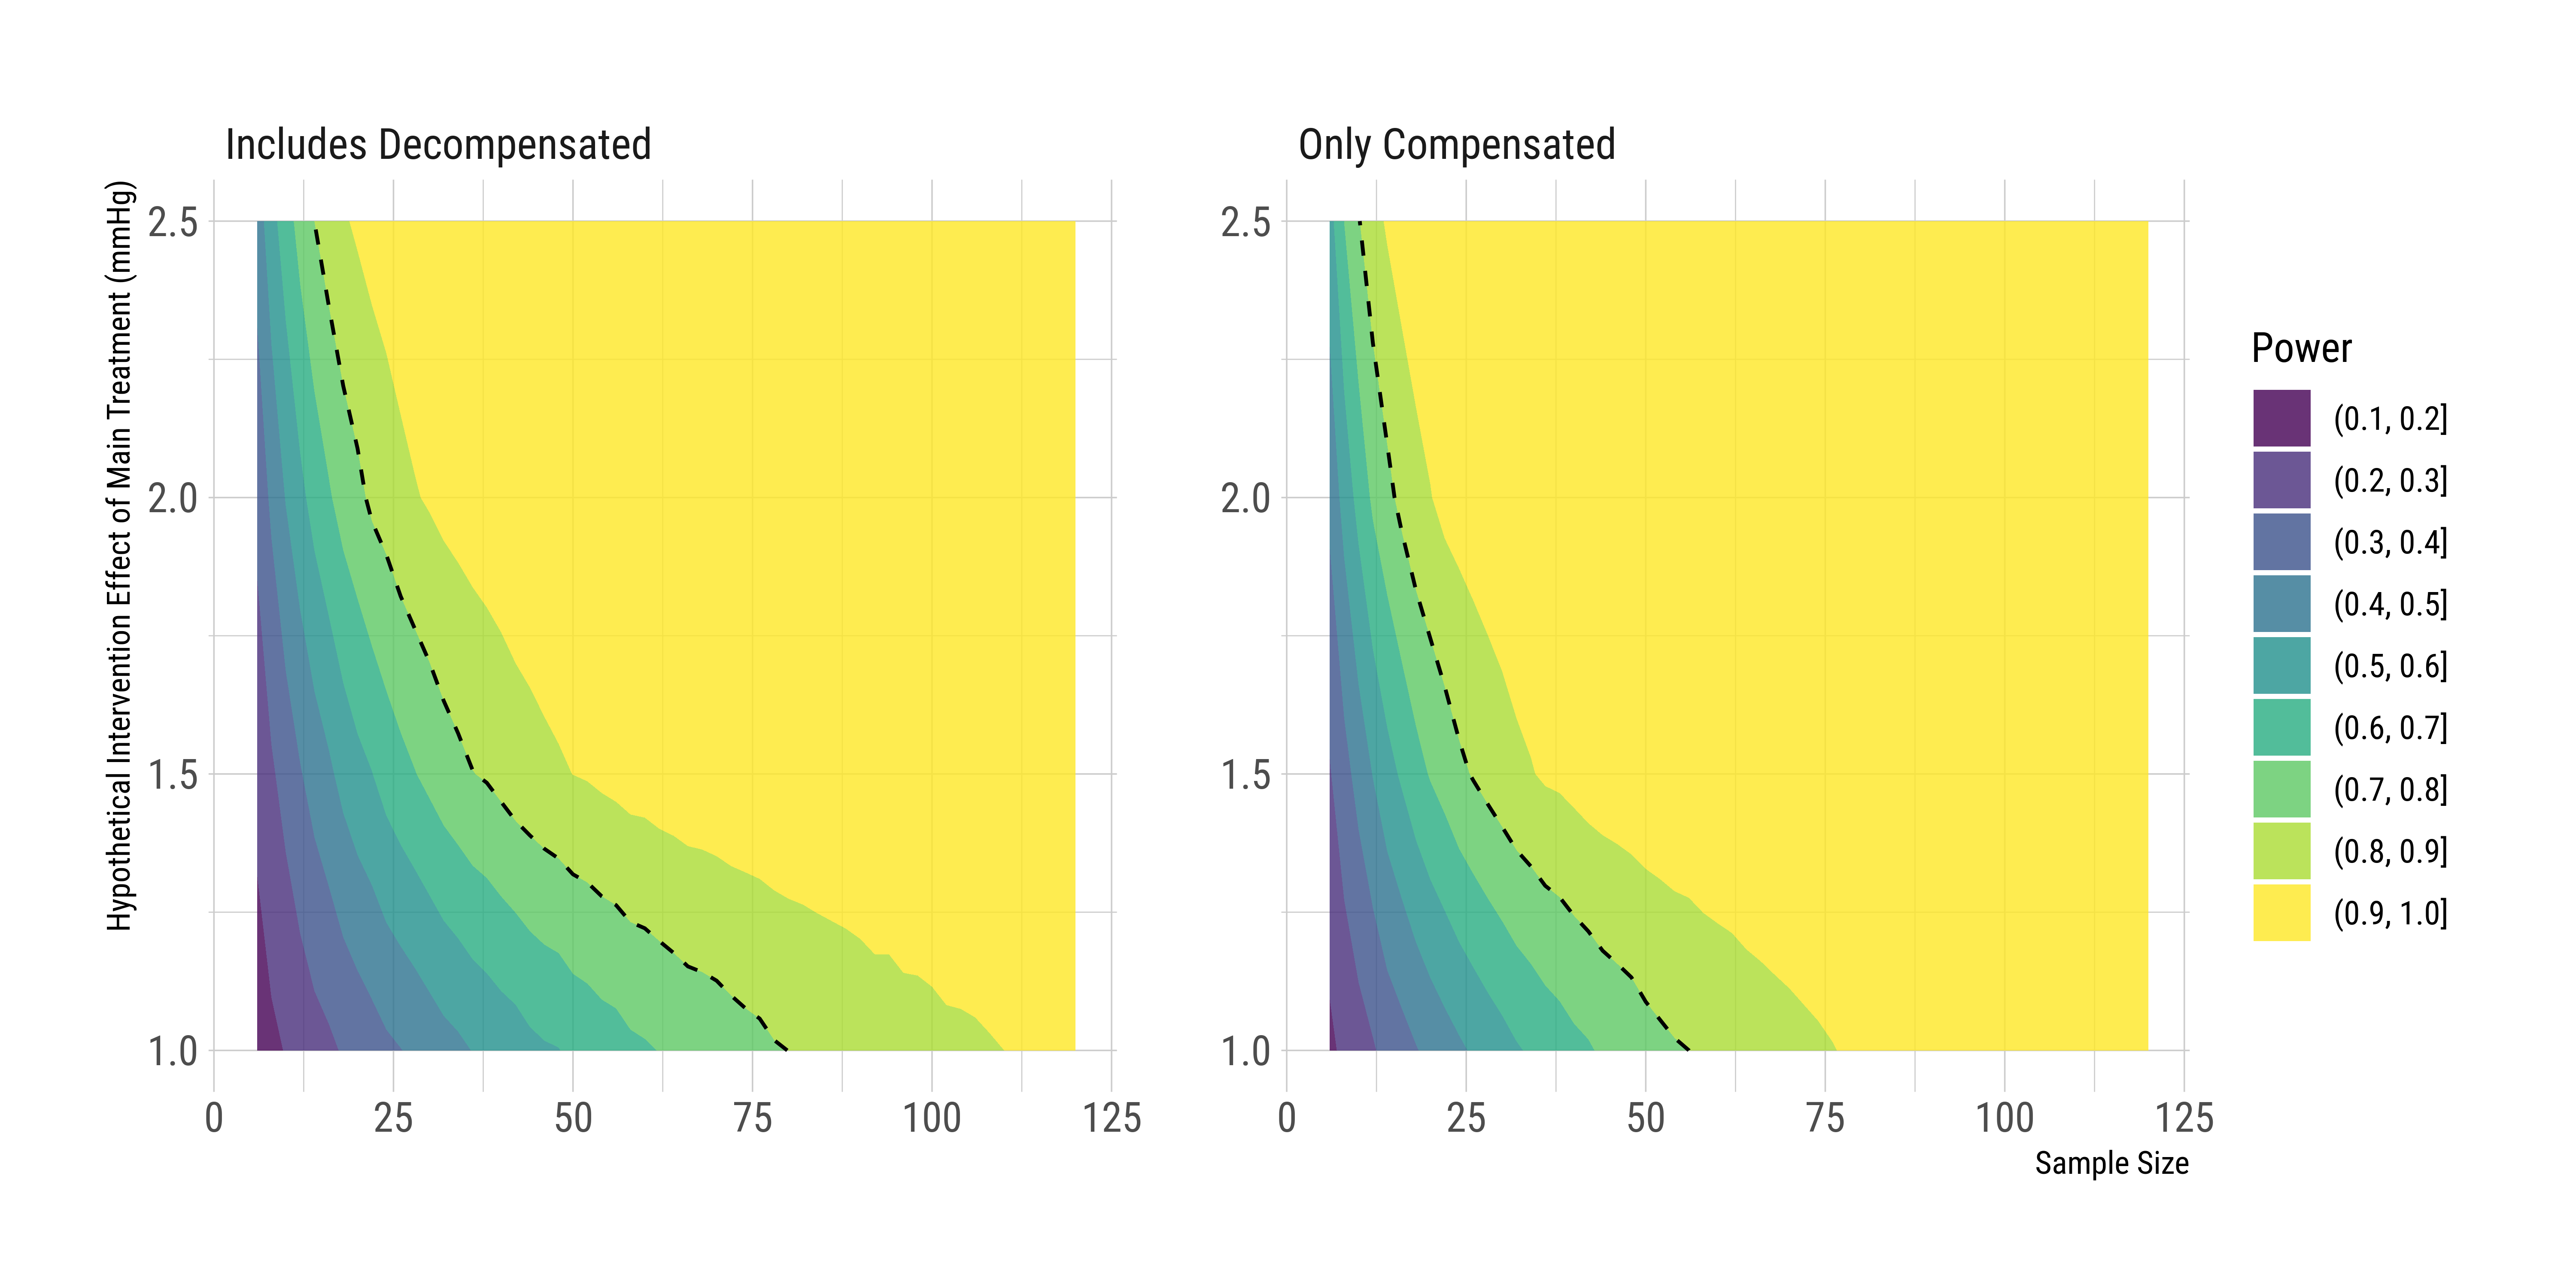
\includegraphics{figures/unnamed-chunk-80-1.png}

\begin{Shaded}
\begin{Highlighting}[]
\NormalTok{difindif\_cont3\_het }\OtherTok{\textless{}{-}}\NormalTok{ difindifsims\_res\_het }\SpecialCharTok{\%\textgreater{}\%} 
  \FunctionTok{filter}\NormalTok{(deltadif}\SpecialCharTok{!=}\DecValTok{3}\NormalTok{) }\SpecialCharTok{\%\textgreater{}\%} 
  \FunctionTok{filter}\NormalTok{(delta2}\SpecialCharTok{==}\DecValTok{0}\NormalTok{) }\SpecialCharTok{\%\textgreater{}\%} 
  \FunctionTok{ggplot}\NormalTok{(}\FunctionTok{aes}\NormalTok{(}\AttributeTok{x=}\NormalTok{n, }\AttributeTok{y=}\NormalTok{delta1, }\AttributeTok{z=}\NormalTok{power)) }\SpecialCharTok{+}
  \FunctionTok{geom\_contour\_filled}\NormalTok{(}\AttributeTok{alpha=}\FloatTok{0.8}\NormalTok{, }\AttributeTok{breaks=}\FunctionTok{seq}\NormalTok{(}\DecValTok{0}\NormalTok{,}\FloatTok{1.1}\NormalTok{, }\AttributeTok{by=}\FloatTok{0.1}\NormalTok{)) }\SpecialCharTok{+}
  \FunctionTok{facet\_wrap}\NormalTok{(.}\SpecialCharTok{\textasciitilde{}}\NormalTok{decomp, }\AttributeTok{scales =} \StringTok{"free"}\NormalTok{) }\SpecialCharTok{+}
  \FunctionTok{theme\_ipsum\_rc}\NormalTok{() }\SpecialCharTok{+}
  \FunctionTok{labs}\NormalTok{(}\AttributeTok{x =} \StringTok{"Sample Size"}\NormalTok{,}
       \AttributeTok{y =} \StringTok{"Hypothetical Intervention Effect of Main Treatment (mmHg)"}\NormalTok{) }\SpecialCharTok{+}
  \FunctionTok{scale\_y\_continuous}\NormalTok{(}\AttributeTok{breaks =} \FunctionTok{seq}\NormalTok{(}\FloatTok{0.5}\NormalTok{, }\DecValTok{5}\NormalTok{, }\AttributeTok{by =} \FloatTok{0.5}\NormalTok{)) }\SpecialCharTok{+}
  \FunctionTok{scale\_fill\_viridis}\NormalTok{(}\StringTok{"Power"}\NormalTok{, }\AttributeTok{discrete =}\NormalTok{ T) }\SpecialCharTok{+}
  \FunctionTok{geom\_contour}\NormalTok{(}\AttributeTok{breaks=}\FloatTok{0.8}\NormalTok{, }\AttributeTok{colour=}\StringTok{"black"}\NormalTok{, }\AttributeTok{linetype=}\StringTok{"dashed"}\NormalTok{) }\SpecialCharTok{+}
  \FunctionTok{xlim}\NormalTok{(}\FunctionTok{c}\NormalTok{(}\DecValTok{5}\NormalTok{,}\DecValTok{120}\NormalTok{))}

\NormalTok{difindif\_cont3\_het}
\end{Highlighting}
\end{Shaded}

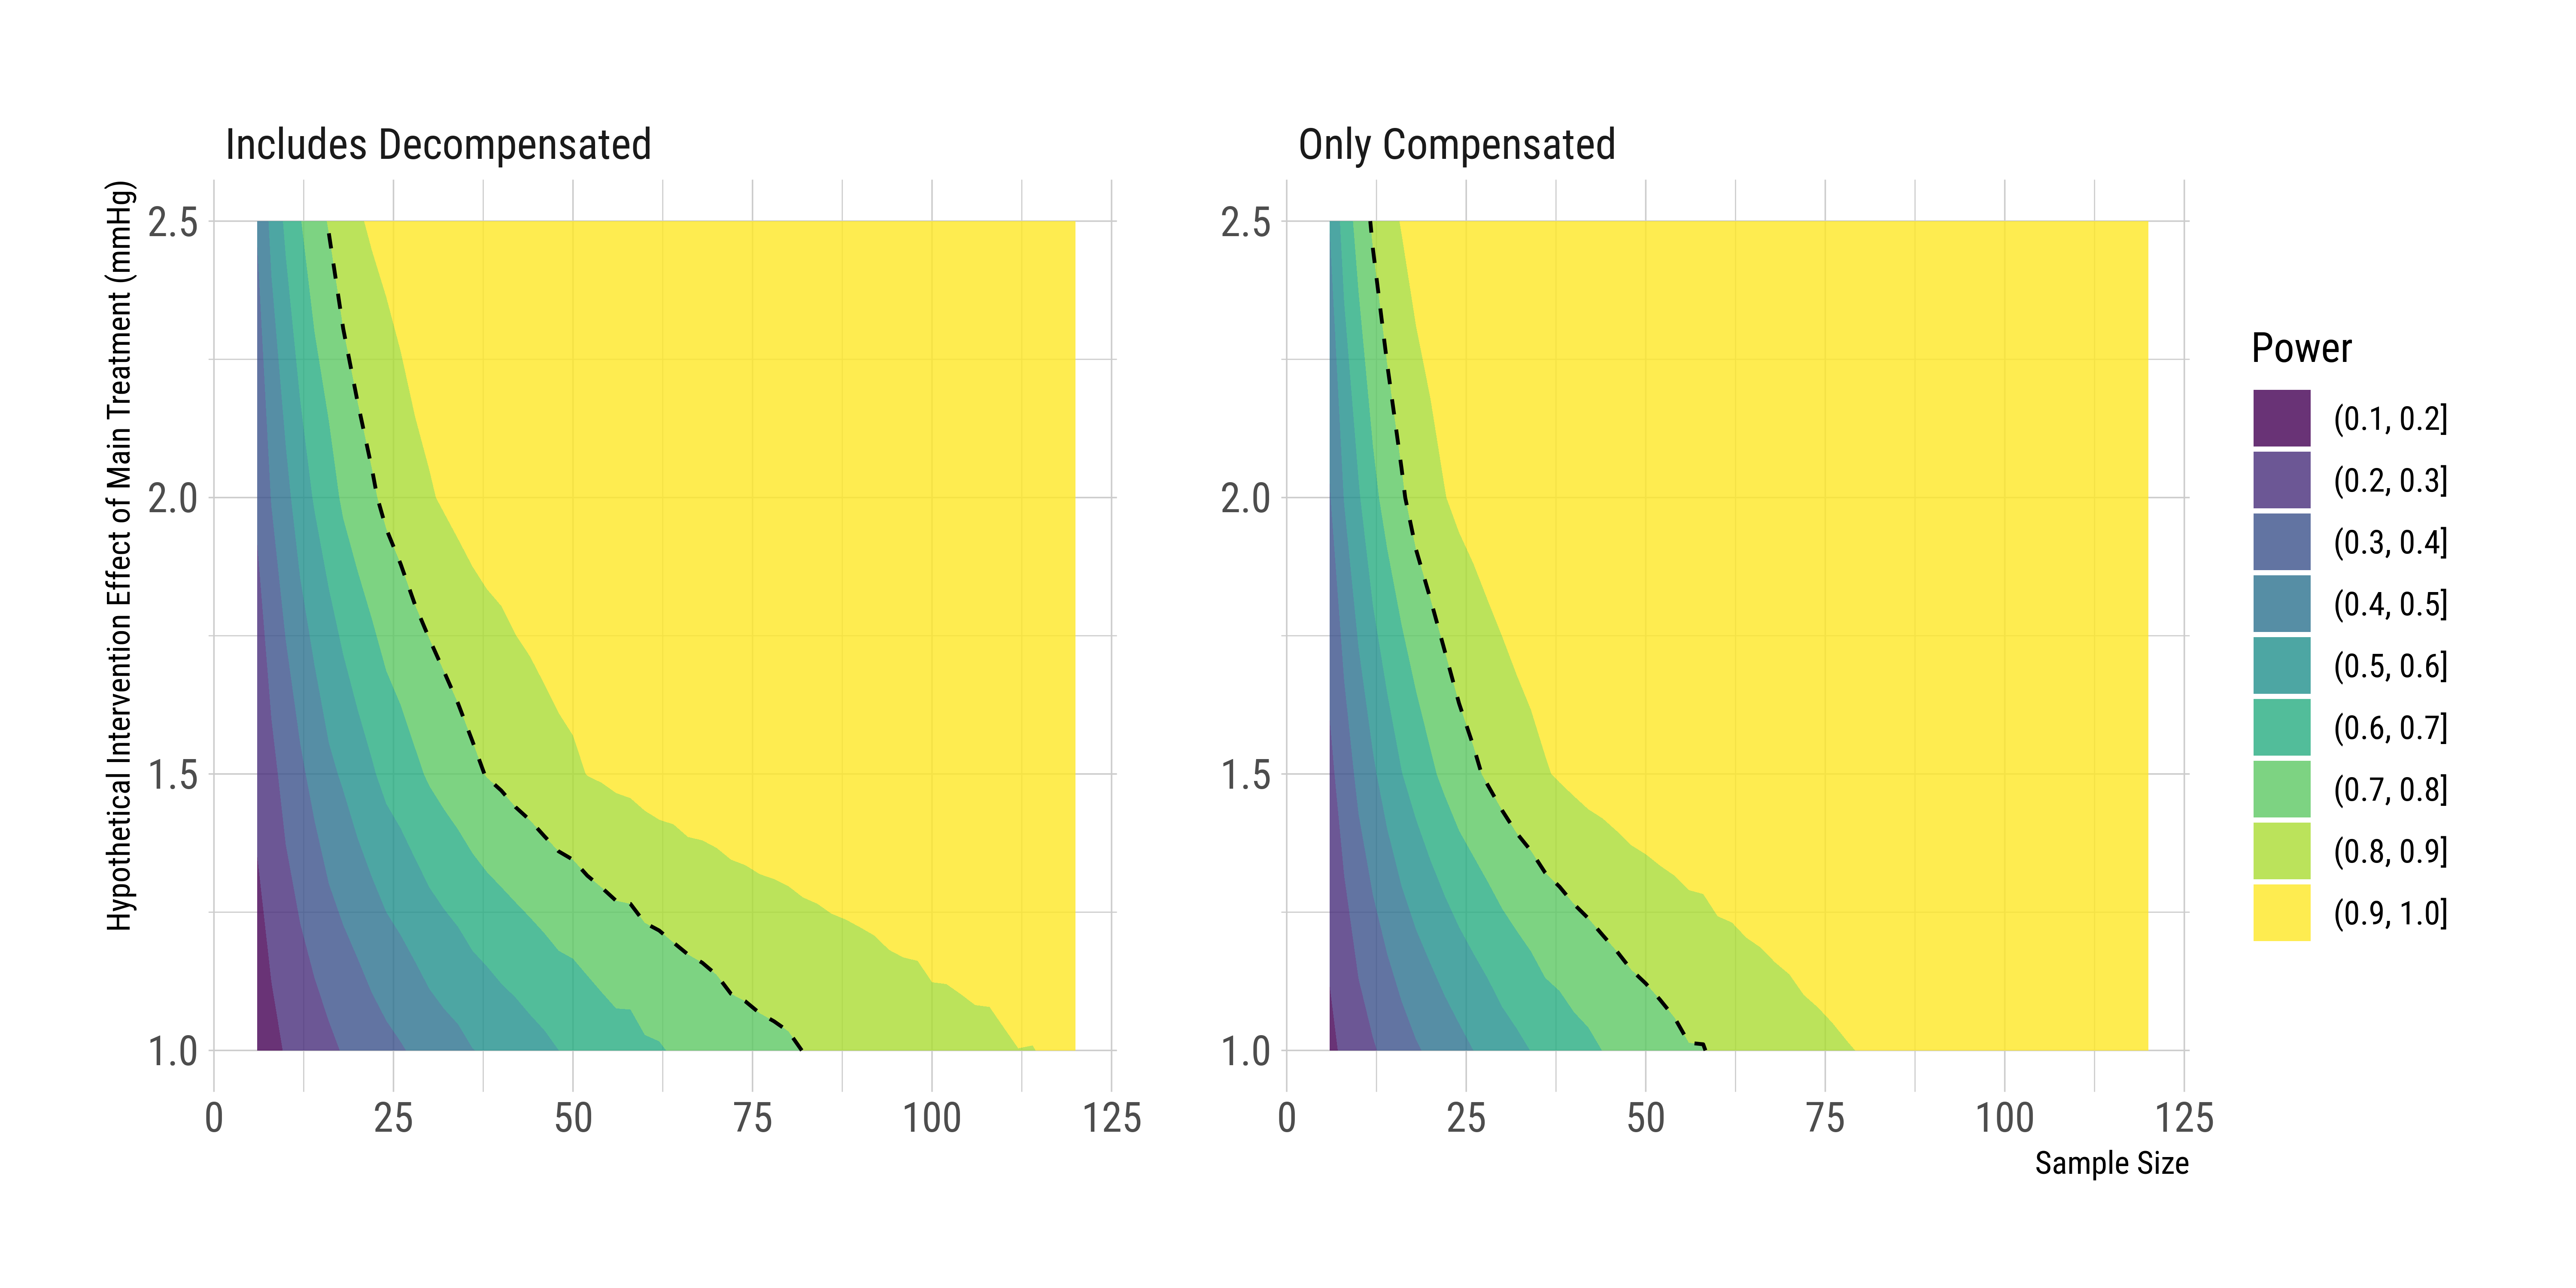
\includegraphics{figures/unnamed-chunk-80-2.png}

\begin{Shaded}
\begin{Highlighting}[]
\FunctionTok{ggsave}\NormalTok{(difindif\_cont3\_hom, }\AttributeTok{height=}\DecValTok{5}\NormalTok{, }\AttributeTok{width=}\DecValTok{10}\NormalTok{, }\AttributeTok{filename =} \StringTok{"figures/Difindif\_hom\_contour.png"}\NormalTok{)}
\FunctionTok{ggsave}\NormalTok{(difindif\_cont3\_het, }\AttributeTok{height=}\DecValTok{5}\NormalTok{, }\AttributeTok{width=}\DecValTok{10}\NormalTok{, }\AttributeTok{filename =} \StringTok{"figures/Difindif\_het\_contour.png"}\NormalTok{)}

\FunctionTok{ggsave}\NormalTok{(difindif\_cont3\_hom, }\AttributeTok{height=}\DecValTok{5}\NormalTok{, }\AttributeTok{width=}\DecValTok{10}\NormalTok{, }\AttributeTok{filename =} \StringTok{"figures/Difindif\_hom\_contour.jpg"}\NormalTok{, }
       \AttributeTok{dpi =} \DecValTok{600}\NormalTok{)}
\FunctionTok{ggsave}\NormalTok{(difindif\_cont3\_het, }\AttributeTok{height=}\DecValTok{5}\NormalTok{, }\AttributeTok{width=}\DecValTok{10}\NormalTok{, }\AttributeTok{filename =} \StringTok{"figures/Difindif\_het\_contour.jpg"}\NormalTok{, }
       \AttributeTok{dpi =} \DecValTok{600}\NormalTok{)}
\end{Highlighting}
\end{Shaded}

\hypertarget{icc-figures}{%
\section{ICC Figures}\label{icc-figures}}

\begin{Shaded}
\begin{Highlighting}[]
\NormalTok{colours }\OtherTok{\textless{}{-}} \FunctionTok{c}\NormalTok{(}\StringTok{"\#61b096"}\NormalTok{, }\StringTok{"\#bd7969"}\NormalTok{)}

\NormalTok{make\_distributions }\OtherTok{\textless{}{-}} \ControlFlowTok{function}\NormalTok{(icc) \{}
  
\NormalTok{  sd\_true }\OtherTok{\textless{}{-}} \DecValTok{1}
\NormalTok{  var\_true }\OtherTok{\textless{}{-}}\NormalTok{ sd\_true}\SpecialCharTok{\^{}}\DecValTok{2}
  
\NormalTok{  var\_tot }\OtherTok{\textless{}{-}}\NormalTok{ var\_true }\SpecialCharTok{/}\NormalTok{ icc}
\NormalTok{  sd\_tot }\OtherTok{\textless{}{-}} \FunctionTok{sqrt}\NormalTok{(var\_tot)}
  
\NormalTok{  sd\_error }\OtherTok{\textless{}{-}} \FunctionTok{sqrt}\NormalTok{(var\_tot }\SpecialCharTok{{-}}\NormalTok{ var\_true)}
  
\NormalTok{  distrib }\OtherTok{\textless{}{-}} \FunctionTok{ggplot}\NormalTok{(}\FunctionTok{data.frame}\NormalTok{(}\AttributeTok{x=}\FunctionTok{c}\NormalTok{(}\SpecialCharTok{{-}}\DecValTok{5}\NormalTok{,}\DecValTok{5}\NormalTok{)), }\FunctionTok{aes}\NormalTok{(}\AttributeTok{x=}\NormalTok{x)) }\SpecialCharTok{+}
      \FunctionTok{stat\_function}\NormalTok{(}\AttributeTok{fun =}\NormalTok{ dnorm, }
        \AttributeTok{colour =} \StringTok{"black"}\NormalTok{, }\AttributeTok{size =} \FloatTok{1.5}\NormalTok{, }\AttributeTok{args =} \FunctionTok{list}\NormalTok{(}\AttributeTok{mean =} \DecValTok{0}\NormalTok{, }\AttributeTok{sd=}\NormalTok{sd\_tot), }
        \AttributeTok{geom =} \StringTok{"line"}\NormalTok{) }\SpecialCharTok{+}
    \FunctionTok{stat\_function}\NormalTok{(}\AttributeTok{fun =}\NormalTok{ dnorm, }
        \AttributeTok{colour =}\NormalTok{ colours[}\DecValTok{1}\NormalTok{], }\AttributeTok{size =} \DecValTok{1}\NormalTok{, }\AttributeTok{args =} \FunctionTok{list}\NormalTok{(}\AttributeTok{mean =} \DecValTok{0}\NormalTok{, }\AttributeTok{sd=}\NormalTok{sd\_true), }
        \AttributeTok{geom =} \StringTok{"line"}\NormalTok{) }\SpecialCharTok{+}
    \FunctionTok{stat\_function}\NormalTok{(}\AttributeTok{fun =}\NormalTok{ dnorm, }
        \AttributeTok{colour =}\NormalTok{ colours[}\DecValTok{2}\NormalTok{], }\AttributeTok{size =} \DecValTok{1}\NormalTok{, }\AttributeTok{args =} \FunctionTok{list}\NormalTok{(}\AttributeTok{mean =} \DecValTok{0}\NormalTok{, }\AttributeTok{sd=}\NormalTok{sd\_error), }
        \AttributeTok{geom =} \StringTok{"line"}\NormalTok{) }\SpecialCharTok{+}
    \FunctionTok{geom\_vline}\NormalTok{(}\AttributeTok{xintercept =} \DecValTok{0}\NormalTok{, }\AttributeTok{linetype=}\StringTok{"dashed"}\NormalTok{) }\SpecialCharTok{+}
    \FunctionTok{theme}\NormalTok{(}\AttributeTok{axis.title.x =} \FunctionTok{element\_blank}\NormalTok{(),}
          \AttributeTok{axis.title.y =} \FunctionTok{element\_blank}\NormalTok{(),}
          \AttributeTok{axis.text.y=}\FunctionTok{element\_blank}\NormalTok{(),}
          \AttributeTok{axis.ticks.y=}\FunctionTok{element\_blank}\NormalTok{(),}
          \AttributeTok{axis.text.x=}\FunctionTok{element\_blank}\NormalTok{(),}
          \AttributeTok{panel.grid.major =} \FunctionTok{element\_blank}\NormalTok{(), }
          \AttributeTok{panel.grid.minor =} \FunctionTok{element\_blank}\NormalTok{()) }\SpecialCharTok{+}
    \FunctionTok{annotate}\NormalTok{(}\StringTok{"text"}\NormalTok{, }\AttributeTok{x=}\FloatTok{2.5}\NormalTok{, }\AttributeTok{y=}\FloatTok{0.5}\NormalTok{, }
           \AttributeTok{label=}\StringTok{"Error}\SpecialCharTok{\textbackslash{}n}\StringTok{Variance"}\NormalTok{,}
           \AttributeTok{colour =}\NormalTok{ colours[}\DecValTok{2}\NormalTok{], }\AttributeTok{hjust=}\FloatTok{0.5}\NormalTok{) }\SpecialCharTok{+}
    \FunctionTok{annotate}\NormalTok{(}\StringTok{"text"}\NormalTok{, }\AttributeTok{x=}\SpecialCharTok{{-}}\FloatTok{2.5}\NormalTok{, }\AttributeTok{y=}\FloatTok{0.5}\NormalTok{, }
           \AttributeTok{label=}\StringTok{"True}\SpecialCharTok{\textbackslash{}n}\StringTok{Variance"}\NormalTok{,}
           \AttributeTok{colour =}\NormalTok{ colours[}\DecValTok{1}\NormalTok{], }\AttributeTok{hjust=}\FloatTok{0.5}\NormalTok{) }\SpecialCharTok{+}
    \FunctionTok{coord\_cartesian}\NormalTok{(}\AttributeTok{ylim=}\FunctionTok{c}\NormalTok{(}\DecValTok{0}\NormalTok{,}\FloatTok{0.7}\NormalTok{))}
  
  \FunctionTok{return}\NormalTok{(distrib)}
\NormalTok{\}}

\NormalTok{make\_piecharts }\OtherTok{\textless{}{-}} \ControlFlowTok{function}\NormalTok{(icc) \{}
  
\NormalTok{  sd\_true }\OtherTok{\textless{}{-}} \DecValTok{1}
\NormalTok{  var\_true }\OtherTok{\textless{}{-}}\NormalTok{ sd\_true}\SpecialCharTok{\^{}}\DecValTok{2}
  
\NormalTok{  var\_tot }\OtherTok{\textless{}{-}}\NormalTok{ var\_true }\SpecialCharTok{/}\NormalTok{ icc}
\NormalTok{  sd\_tot }\OtherTok{\textless{}{-}} \FunctionTok{sqrt}\NormalTok{(var\_tot)}
  
\NormalTok{  var\_error }\OtherTok{\textless{}{-}}\NormalTok{ var\_tot }\SpecialCharTok{{-}}\NormalTok{ var\_true}
  
\NormalTok{  var\_pie }\OtherTok{\textless{}{-}} \FunctionTok{data.frame}\NormalTok{(}\AttributeTok{Variance =} \FunctionTok{c}\NormalTok{(}\StringTok{"True"}\NormalTok{, }\StringTok{"Error"}\NormalTok{),}
                \AttributeTok{Values =} \FunctionTok{c}\NormalTok{(var\_true, var\_error))}
\NormalTok{  var\_pie}\SpecialCharTok{$}\NormalTok{Variance }\OtherTok{\textless{}{-}}\NormalTok{ forcats}\SpecialCharTok{::}\FunctionTok{fct\_inorder}\NormalTok{(var\_pie}\SpecialCharTok{$}\NormalTok{Variance)}
  
  
\NormalTok{  pie }\OtherTok{\textless{}{-}} \FunctionTok{ggplot}\NormalTok{(var\_pie, }\FunctionTok{aes}\NormalTok{(}\AttributeTok{x=}\StringTok{""}\NormalTok{, }\AttributeTok{y=}\NormalTok{Values, }\AttributeTok{fill=}\NormalTok{Variance))}\SpecialCharTok{+}
    \FunctionTok{geom\_bar}\NormalTok{(}\AttributeTok{width =} \DecValTok{1}\NormalTok{, }\AttributeTok{stat =} \StringTok{"identity"}\NormalTok{) }\SpecialCharTok{+}
    \FunctionTok{theme}\NormalTok{(}\AttributeTok{axis.text.y=}\FunctionTok{element\_blank}\NormalTok{(),}
          \AttributeTok{axis.ticks.y=}\FunctionTok{element\_blank}\NormalTok{(),}
          \AttributeTok{axis.text.x=}\FunctionTok{element\_blank}\NormalTok{(),}
          \AttributeTok{axis.ticks.x=}\FunctionTok{element\_blank}\NormalTok{(),}
          \AttributeTok{panel.grid.major =} \FunctionTok{element\_blank}\NormalTok{(), }
          \AttributeTok{panel.grid.minor =} \FunctionTok{element\_blank}\NormalTok{()) }\SpecialCharTok{+}
    \FunctionTok{coord\_polar}\NormalTok{(}\StringTok{"y"}\NormalTok{, }\AttributeTok{start=}\DecValTok{0}\NormalTok{) }\SpecialCharTok{+}
    \FunctionTok{scale\_fill\_manual}\NormalTok{(}\AttributeTok{values =}\NormalTok{ colours) }\SpecialCharTok{+}
    \FunctionTok{labs}\NormalTok{(}\AttributeTok{x=}\StringTok{""}\NormalTok{, }\AttributeTok{y=}\StringTok{""}\NormalTok{) }\SpecialCharTok{+}
    \FunctionTok{guides}\NormalTok{(}\AttributeTok{fill=}\ConstantTok{FALSE}\NormalTok{) }\SpecialCharTok{+}
    \CommentTok{\#labs(title=paste0("ICC=", icc)) +}
    \ConstantTok{NULL}
    
  
  \FunctionTok{return}\NormalTok{(pie)}
\NormalTok{\}}

\NormalTok{make\_distrib\_and\_pie }\OtherTok{\textless{}{-}} \ControlFlowTok{function}\NormalTok{(icc) \{}
  
\NormalTok{  dist }\OtherTok{\textless{}{-}} \FunctionTok{make\_distributions}\NormalTok{(icc)}
\NormalTok{  pie }\OtherTok{\textless{}{-}} \FunctionTok{make\_piecharts}\NormalTok{(icc)}
  
\NormalTok{  outplot }\OtherTok{\textless{}{-}}\NormalTok{ cowplot}\SpecialCharTok{::}\FunctionTok{plot\_grid}\NormalTok{(pie, dist, }\AttributeTok{rel\_widths =} \FunctionTok{c}\NormalTok{(}\DecValTok{1}\NormalTok{,}\DecValTok{2}\NormalTok{)) }\SpecialCharTok{+}
    \FunctionTok{draw\_figure\_label}\NormalTok{(}\FunctionTok{paste0}\NormalTok{(}\StringTok{"ICC="}\NormalTok{, icc))}
  
  \FunctionTok{return}\NormalTok{(outplot)}
  
\NormalTok{\}}

\NormalTok{comparison\_charts }\OtherTok{\textless{}{-}} \FunctionTok{tibble}\NormalTok{(}
  \AttributeTok{icc =} \FunctionTok{c}\NormalTok{(}\FloatTok{0.1}\NormalTok{, }\FloatTok{0.3}\NormalTok{, }\FloatTok{0.7}\NormalTok{, }\FloatTok{0.9}\NormalTok{)}
\NormalTok{) }\SpecialCharTok{\%\textgreater{}\%} 
  \FunctionTok{mutate}\NormalTok{(}\AttributeTok{chart =}\NormalTok{ purrr}\SpecialCharTok{::}\FunctionTok{map}\NormalTok{(icc, make\_distrib\_and\_pie))}

\FunctionTok{plot\_grid}\NormalTok{(}\AttributeTok{plotlist =}\NormalTok{ comparison\_charts}\SpecialCharTok{$}\NormalTok{chart, }\AttributeTok{ncol=}\DecValTok{1}\NormalTok{)}
\end{Highlighting}
\end{Shaded}

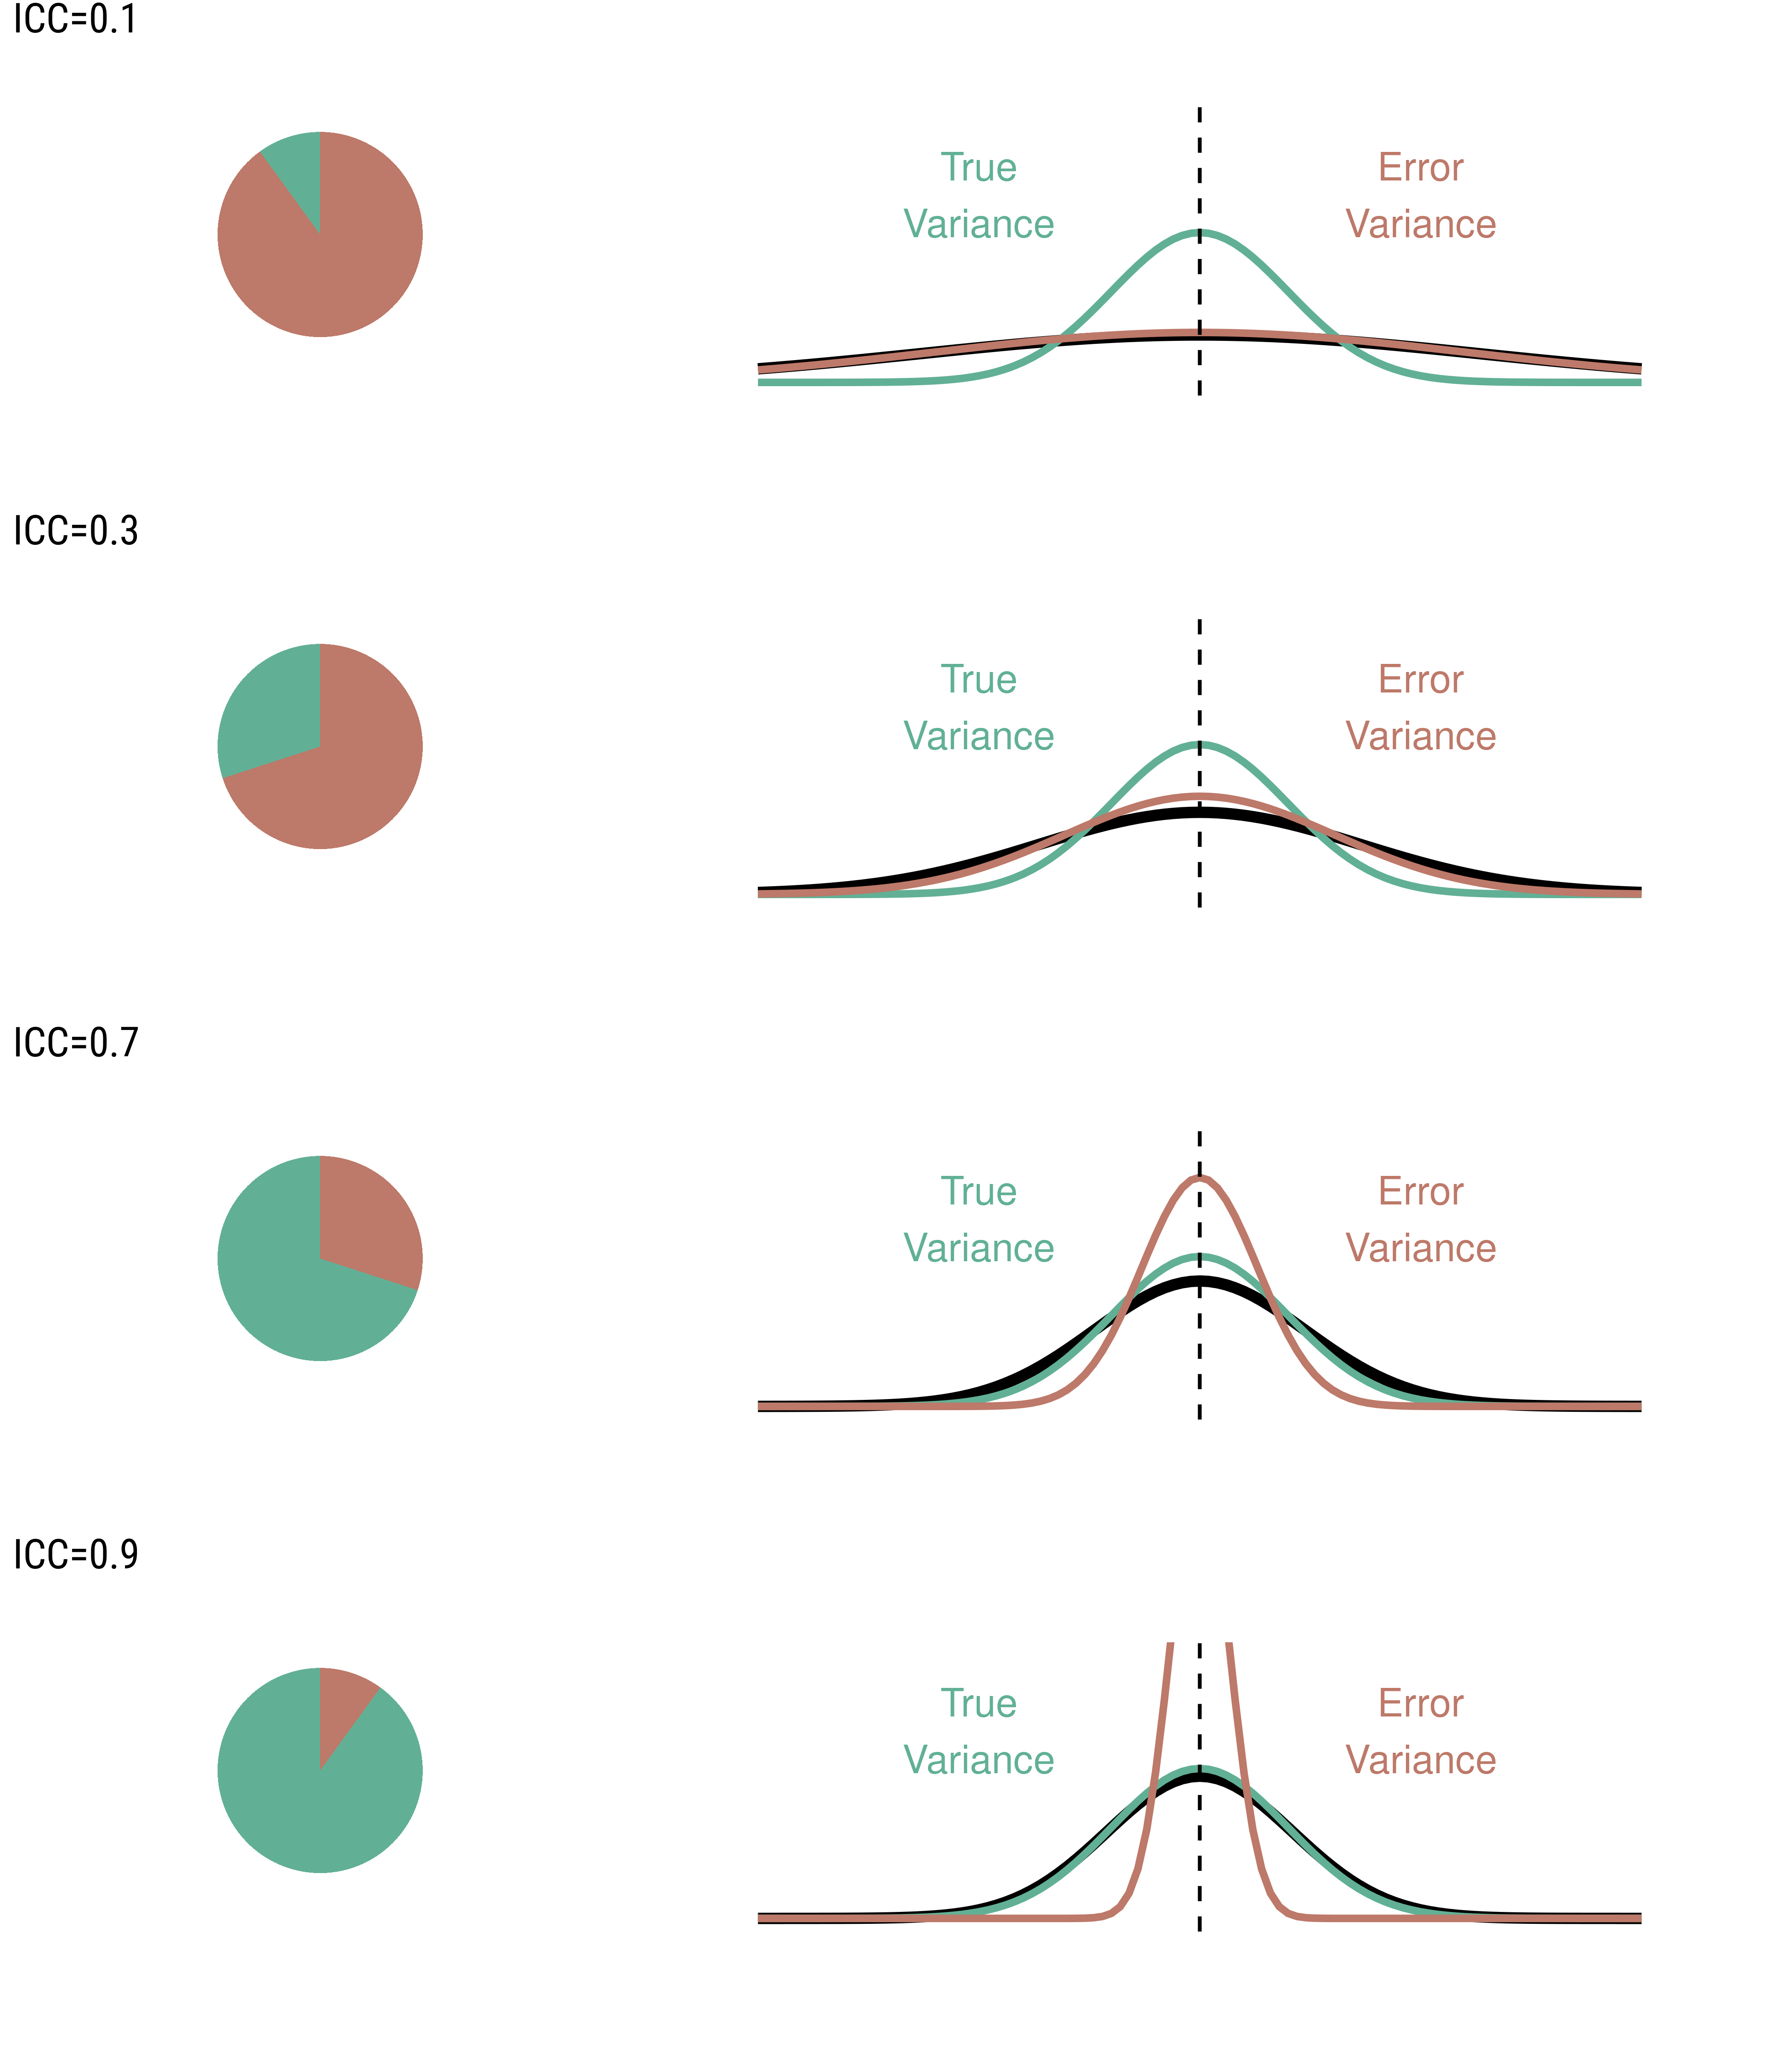
\includegraphics{figures/icc_distribs-1.png}

\end{document}
